\input{glyphtounicode-cmex}
\pdfgentounicode=1
\pdfglyphtounicode{tfm:esint10/acute}{222B}
\pdfglyphtounicode{tfm:esint10/circumflex}{222B}
\pdfglyphtounicode{tfm:esint10/dieresis}{222C}
\pdfglyphtounicode{tfm:esint10/ffl}{2A0F}
\pdfglyphtounicode{tfm:esint10/space}{2A0F}
\documentclass[11pt]{article}
\usepackage[T1]{fontenc}
\usepackage{lmodern}
\usepackage[margin=1in]{geometry}
\usepackage{amsmath,amssymb,amsthm,mathtools,esint}
\usepackage{microtype}
\usepackage{enumitem}
\usepackage{tikz}
\usetikzlibrary{arrows.meta,positioning,calc}
\usepackage[colorlinks=true,linkcolor=blue!50!black,citecolor=blue!50!black,urlcolor=blue!50!black]{hyperref}
\hypersetup{pdftitle={Uniform real Lipschitz surfaces on the triangular lattice},pdfauthor={OpenAI}}
\newtheorem{theorem}{Theorem}[section]
\newtheorem{proposition}[theorem]{Proposition}
\newtheorem{lemma}[theorem]{Lemma}
\newtheorem{corollary}[theorem]{Corollary}
\theoremstyle{definition}
\newtheorem{definition}[theorem]{Definition}
\theoremstyle{remark}
\newtheorem{remark}[theorem]{Remark}
\newcommand{\E}{\mathbb E}
\newcommand{\Prob}{\mathbb P}
\newcommand{\R}{\mathbb R}
\newcommand{\Z}{\mathbb Z}
\newcommand{\dd}{\,\mathrm d}
\newcommand{\eps}{\varepsilon}
\DeclareMathOperator{\dist}{dist}
\DeclareMathOperator{\diam}{diam}
\DeclareMathOperator{\osc}{osc}
\numberwithin{equation}{section}
\title{Uniform real Lipschitz surfaces\\on the triangular lattice}
\author{OpenAI}
\date{October 6, 2026}
\begin{document}
\maketitle
\begin{abstract}
We prove the Gaussian free field and SLE$_4$ scaling limits for uniformly
sampled real nearest-neighbor Lipschitz heights on the triangular lattice,
resolving Schramm's Problem~2.3. On approximations of smooth simply connected
domains, the centered height field converges as a random distribution to a
multiple of the Dirichlet Gaussian free field. At one tuned two-arc boundary
amplitude, the zero-height interface converges in uniform curve distance to
chordal SLE$_4$. We identify the relation between the field variance and the
boundary height in terms of an implicit stationary tangent-flux coefficient.
\end{abstract}
\tableofcontents

\section{The Model and the Theorem}\label{sec:model}
Let $D\subset\R^2$ be a bounded smooth simply connected domain, with
distinct marked boundary points $a,b$. Write $A_+$ and $A_-$ for its
intervening open boundary arcs. The unit triangular lattice has basis
\[
 e_1=(1,0),\qquad e_2=(1/2,\sqrt3/2),
\]
and nearest-neighbor steps $\pm e_1,\pm e_2,\pm(e_1-e_2)$. For mesh
$\delta>0$, take a simply connected triangular-lattice polygon $D_\delta$
whose marked boundary converges uniformly to $(D;a,b)$. Place the two
discrete marks at the midpoints of distinct boundary edges. The resulting
open arcs partition the boundary vertices, so no vertex receives two
boundary values.

For $0<\lambda\le1/2$, let $h_\delta$ have normalized Lebesgue measure on
the set of real vertex heights satisfying
\begin{equation}\label{eq:model}
 h_\delta=\lambda\text{ on }A_{+,\delta},\qquad
 h_\delta=-\lambda\text{ on }A_{-,\delta},\qquad
 |h_\delta(x)-h_\delta(y)|\le1\quad(x\sim y).
\end{equation}
The polytope is bounded because every vertex is at finite graph distance
from the prescribed boundary. In its free coordinates it has nonempty
interior: assigning zero to every free vertex leaves all inequalities
involving a free vertex strict. Fixed--fixed inequalities are already
satisfied by $2\lambda\le1$.

Extend heights affinely across faces. Almost surely no free vertex has
height zero, since that event is a hyperplane of Lebesgue measure zero.
Each triangle then has either no zero segment or a unique segment joining
two edges. These segments form loops and one chordal interface
$\gamma_\delta$ joining the discrete marks. The chord is simple: no face
contains two strands and no vertex is a branching point. Replacing its
within-face placement by the corresponding dual-lattice strand changes
uniform distance by $O(\delta)$.

For continuous curves, use uniform distance modulo increasing
reparametrization:
\[
 d_{\mathrm{unif}}(\alpha,\beta)
 =\inf_{\phi,\psi}\sup_{t\in[0,1]}
       |\alpha(\phi(t))-\beta(\psi(t))|,
\]
where $\phi,\psi$ are increasing homeomorphisms of $[0,1]$, and curves
at zero distance are identified. The Dirichlet GFF convention throughout
is covariance $G_D=(-\Delta_D)^{-1}$.

\begin{theorem}\label{thm:main}
There are constants $A>0$, $\sigma>0$, and $\lambda\in(0,1/2]$, independent
of $D,a,b$, such that the model \eqref{eq:model} has
\[
 \gamma_\delta\Longrightarrow\mathrm{SLE}_4(D;a,b),\qquad
 \frac{h_\delta-\E h_\delta}{\sigma}
       \Longrightarrow\mathrm{GFF}_D
\]
in the stated curve metric and as random distributions, respectively.
The constants and limiting mean are
\begin{align}
 v&=2/\sqrt3,&\sigma^2&=(vA)^{-1},&
 \lambda^2&=\frac{\pi}{8vA},\label{eq:target-constants}\\
 m_D(z)&=\lambda\bigl[\omega_D(z,A_+)-\omega_D(z,A_-)\bigr].&&&
 \label{eq:target-mean}
\end{align}
Here $\omega_D$ is harmonic measure and $A$ is the tangent-flux coefficient
defined in the cell construction. The stiffness is $vA$; no elementary
closed form for it is proposed.
\end{theorem}

The normalization of chordal SLE$_4$ in the half-plane is
$\partial_tg_t(z)=2/(g_t(z)-2B_t)$ with standard real Brownian motion $B$.
There is no logarithmic rescaling of the heights in the distributional
limit. Pointwise height tightness is neither asserted nor required.

\subsection{History and scope}
Schramm's Problem~2.3 asks for SLE$_4$ and GFF limits for this real-valued
hard-constraint model \cite{Schramm}. It is distinct from the integer-valued
model in the preceding problem. Schramm--Sheffield establish the discrete
Gaussian contour result \cite{SSdiscrete}; Miller extends contour
universality to smooth symmetric uniformly convex gradient potentials
\cite{Miller}. The hard potential here is constant on $[-1,1]$ and infinite
outside. It does not satisfy those convexity hypotheses. An approximation
by smooth potentials is therefore not, by itself, a solution.

The identification of effective stiffness and Gaussian fluctuations
belongs to the gradient-field homogenization tradition of Naddaf and
Spencer \cite{NaddafSpencer} and Giacomin, Olla and Spohn
\cite{GiacominOllaSpohn}. For smooth symmetric uniformly convex interactions,
Miller proved a bounded-domain field limit by coupling boundary-conditioned
fields so that their difference is harmonic in the bulk with high probability
\cite{MillerField}. Mi\l o\'s and Peled \cite{MilosPeled}
studied hard-core fluctuations, including the uniform Lipschitz
potential, on even square tori with one pinned height. Their
delocalization and controlled-gradient arguments provide related
finite-volume methods. Cohen-Alloro and Peled's later gradient control
also extends the delocalization argument to square-lattice domains with
zero Dirichlet data \cite[Section~6]{CAP}. These hard-core delocalization
results do not give the
bounded-domain field or contour limits considered here. More recently, Buchholz, Cotar and
Schweiger \cite{BuchholzCotarSchweiger} proved infinite-volume
gradient-field universality for a class of nonconvex potentials.
Their scaling theorem retains smooth, uniformly curved mixture
components and does not cover the flat/infinite hard potential.

The convex-volume foundation uses Pr\'ekopa's integral log-concavity
theorem \cite{Prekopa}; the quantitative facet deficit, triangular
exposure and average anchoring are proved here. The controlled-gradient
estimate of Cohen-Alloro and Peled \cite{CAP} supplies the zero-pinned
starting point. Extending it to bounded data and sign observations
requires separate finite-volume arguments. Those extensions are needed
because an interface exploration continually changes the conditioned
height polytope.

For the finite reflected dynamics we use S\l omi\'nski's fixed-domain
Skorokhod approximation \cite{Slominski}, the Neumann semimartingale
identification of Bass and Hsu \cite{BassHsu}, and the stationary
forward--reverse decomposition of Lyons and Zheng \cite{LyonsZheng}.
The uniform changing-polytope force argument and weighted constant-drift
identification are proved locally. At the curve stage, we adapt the
harmonic-observable method of Schramm and Sheffield \cite{SSdiscrete}
and identify the whole curve using terminal side labels and
harmonic-mass nonreturn. The hard-constraint model supplies its own
conditional covariance, height gap and stopping-time-uniform observable.
These inputs identify both endpoint drivers and their common limiting
arc, and exclude macroscopic backtracking.

\subsection{Plan of the proof}
The proof has four parts. First, local volume curvature and sparse
defects give unscaled moments of macroscopic averages
(Section~\ref{f:section}). Second, synchronous
reflected couplings turn Brownian contact events into weighted control of
differences and their errors at observed sites
(Section~\ref{s:coupling}). Third, the stationary
tangent update identifies a scalar flux law and, through small tilts, a
Gaussian field (Section~\ref{sec:cell}). Analytic trace estimates on
varying observed sets then give conditional Dirichlet covariance
(Sections~\ref{sec:trace-analysis} and~\ref{sec:conditional-covariance}).
Finally, feasible shifts with controlled volume cost turn crossing
estimates into barriers (Section~\ref{sec:feasible-shifts}). These
barriers and conditional field estimates give sampled-interface separation,
then the height gap and the stopped harmonic observable
(Sections~\ref{sec:geometry} and~\ref{sec:interface}).

The demanding uniformity is part of the assertions, not an optional
strengthening: random observations are used only with their exact conditional
Gibbs kernels, and the curve argument needs estimates uniform over the
stopping rules used to test its driving function. In particular,
conditional covariance, survival reweighting, and convergence of labelled
harmonic accesses are established before the driving and whole-curve arguments.

\section{Conventions for the Estimates}\label{sec:conventions}
For local arguments rescale the lattice to spacing one and write $n$ for
the macroscopic length. Discrete edge gradients do not include a factor
$n$. Continuum tests use the Riemann pairing
\[
\langle h,f\rangle_n=\frac1{vn^2}\sum_x f(x/n)h_x.
\]
In the continuum trace sections, the lattice is instead already embedded
at physical mesh $n^{-1}$; there $x$ denotes the physical location and the
same pairing is written with $f(x)$. These are the same normalization.
Constants may depend on a fixed compact test region and on explicitly fixed
scale ratios, but not on $n$ or the microscopic shape of admissible observed
strings. An oriented sign string prescribes the signs adjacent to an
interface piece. Each such vertex has an opposite-sign neighbor, hence its
height belongs to $[-1,1]$. Newly revealed exact values are instead pins;
their annealed estimates must be justified by conditioning, not by treating
arbitrary revealed values as uniformly bounded.

The reflected bath has Brownian variance parameter two in free coordinates
and normal reflection on the convex height polytope. A density tilted by
$\exp(\sum_xb_xh_x)$ adds drift $b$. Finite-dimensional normal-reflection
existence, continuity, invariance of the stated density, and the stationary
forward/reverse martingale decomposition are the standard stochastic tools
used below. Exact-value conditional laws are taken on their almost-sure
positive-volume fibers after the recorded coordinates are removed;
null-volume conditionings are discarded. Reflection and its martingale
decomposition are applied on these free coordinates. The finite-body
references and the separate uniform forcing argument appear in
Section~\ref{s:coupling}.

\section{Local Slack and Macroscopic Averages}\label{f:section}
The estimates in this section provide the spatial compactness and moment
bounds used in the comparison argument. The principal probabilistic input
is the controlled-gradient theorem of Cohen--Alloro and Peled \cite{CAP}.
The local convex-volume argument uses integral log-concavity
\cite[Theorems 3 and 6]{Prekopa}. Its quantitative facet and block
estimates are proved below for the present triangular lattice.

\subsection{The finite-volume laws and the moment statement}
We identify the triangular lattice with $\mathbb Z^2$, with edges in the
directions $\pm e_1,\pm e_2,\pm(e_1-e_2)$. Distances are graph distances.
Let $V$ be a finite set of free vertices, and prescribe height zero on its
exterior vertex boundary and on any additional pins. Write $\mu_0$ for
uniform Lebesgue measure on the remaining heights satisfying the edge
constraints. A zero-pinned sample is extended by zero to the whole lattice.
Its defining polytope is compact and has positive volume on its free
coordinates. A bounded-data law $\mu_b$ has the same fixed set and prescribed
values $b$ with $|b|\le B$, and is considered only when its polytope has
positive volume. Constants below are independent of the number and shape
of the components of $V$.

\begin{proposition}[Macroscopic exponential moments]\label{f:averages}
Fix $c,C>0$ and $B<\infty$. Let $R\ge1$ and let deterministic real weights
$q_x$ obey
\begin{equation}\label{f:weights}
 \sum_x|q_x|\le C,\qquad \max_x|q_x|\le CR^{-2},\qquad
 \operatorname{supp}q\subset Q,
 \quad \operatorname{diam}Q\le CR,
\end{equation}
where $Q$ is an ambient coordinate box. Assume either $\sum_xq_x=0$, or
there is a connected set of pins $K$, of diameter at least $cR$, such that
$K\cup Q$ lies in a coordinate box of diameter at most $CR$. For a sample
$h$ from $\mu_b$, there are $a>0$ and $M<\infty$, depending only on
$c,C,B$, such that
\begin{equation}\label{f:average-mgf}
 \E\exp\left(a\left|\sum_xq_xh(x)\right|\right)\le M.
\end{equation}
The conclusion is uniform over mixtures of bounded pin values whenever
conditioning on those values leaves exactly the specified uniform law.
\end{proposition}

The zero-mass alternative covers differences of comparable-scale averages
in a free ball even when the nearest pin is much farther away. An ordinary
ball average, or a smooth average of that scale, satisfies
\eqref{f:weights}. Restriction of its original positive weights to the
domain also satisfies that condition. Renormalization after restriction
requires a new verification of the bound $\max|q_x|\le CR^{-2}$.
We first prove the proposition for zero pins. The proof will also identify
the exact deterministic estimates required of later comparison fields.

\subsection{A local filling-volume deficit}
Fix a large even integer $L$ and tile the lattice by
$Q_z=Lz+\{0,\ldots,L\}^2$. The interiors of distinct blocks have no
connecting edge. For shell data $s$ on $\partial Q$, let $K_Q(s)$ be the
polytope of fillings and put
\[
 F_Q(s)=\log\operatorname{vol}_{(L-1)^2}K_Q(s),
\]
with value $-\infty$ when the volume is zero. The inclusion
$\frac12(K_Q(s_1)+K_Q(s_2))\subset K_Q((s_1+s_2)/2)$ and
Brunn--Minkowski imply concavity of $F_Q$.

Concavity gives a nonnegative midpoint loss. We next show that, on blocks
with slack, this loss controls differences between the perturbations of
the shell heights at the four side midpoints. It cannot control a common
height shift, which leaves filling volume unchanged. The later coarse-grid
argument combines these differences; the connected pins or the zero-mass
hypothesis in Proposition~\ref{f:averages} remove the additive constant.

For each of the four sides, let $v$ be its midpoint and let $r$ be
the coordinate unit step pointing toward the block center. The inward
path is $v+kr$, $0\le k\le L/2$. Of the two tangential unit steps
on that side, let $t$ be the one with $r\cdot t=1/2$. The
\emph{compressed ray} is $v+\ell t$, $0\le\ell\le L/2$:
its graph distance to $v+kr$ is $\max(k,\ell)$. These choices define
the four tests below. Figure~\ref{fig:triangular} illustrates one of them.

For fixed $0<\delta\le\delta_0\le1/16$, an integer $k_0\ge4/\delta_0$,
and $s_0>0$, call a block \emph{convex-good} for $h$ if
\begin{align}
 |h(x)-h(y)|&\le1-\delta &&(x\sim y\text{ in }Q),\label{f:near}\\
 |h(x)-h(y)|&\le(1-\delta_0)\operatorname{dist}(x,y)
 &&(x,y\in Q,\ \operatorname{dist}(x,y)\ge k_0),\label{f:far}
\end{align}
and the following four non-tie conditions hold. For each face center $v$,
take the radial coordinate path from $v$ to the block center. Exactly one
ray on its starting face has compressed triangular distances to that path;
if $b_1$ is its first vertex, require $|h(b_1)-h(v)|\ge s_0$.
Take $L\ge8(k_0+2)/\delta_0$.

\begin{figure}[ht]
\centering
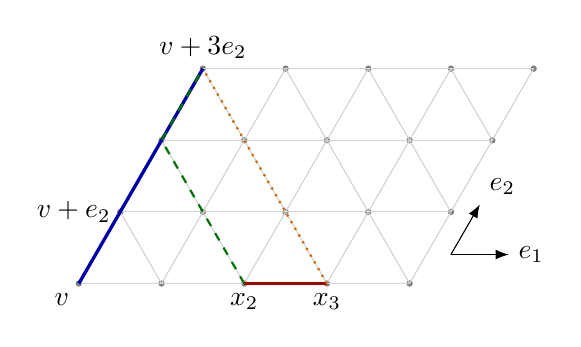
\begin{tikzpicture}[scale=1.05,>=Latex]
\foreach \i in {0,...,4} {
  \foreach \j in {0,...,3} {
    \coordinate (v\i\j) at ({\i+0.5*\j},{0.8660254*\j});
    \fill[gray] (v\i\j) circle (1.1pt);
  }
}
\foreach \i in {0,...,3} {
  \foreach \j in {0,...,3} {
    \draw[gray!35] ({\i+0.5*\j},{0.8660254*\j}) --
      ({\i+1+0.5*\j},{0.8660254*\j});
  }
}
\foreach \i in {0,...,4} {
  \foreach \j in {0,...,2} {
    \draw[gray!35] ({\i+0.5*\j},{0.8660254*\j}) --
      ({\i+0.5*(\j+1)},{0.8660254*(\j+1)});
  }
}
\foreach \i in {0,...,3} {
  \foreach \j in {0,...,2} {
    \draw[gray!35] ({\i+1+0.5*\j},{0.8660254*\j}) --
      ({\i+0.5*(\j+1)},{0.8660254*(\j+1)});
  }
}
\draw[blue!65!black,very thick] (v00)--(v03);
\draw[red!65!black,very thick] (v20)--(v30);
\draw[green!45!black,thick,dashed] (v20)--(v11)--(v02)--(v03);
\draw[orange!80!black,thick,dotted] (v30)--(v21)--(v12)--(v03);
\node[below left] at (v00) {$v$};
\node[left] at (v01) {$v+e_2$};
\node[above] at (v03) {$v+3e_2$};
\node[below] at (v20) {$x_2$};
\node[below] at (v30) {$x_3$};
\draw[->] (4.5,0.35)--(5.2,0.35) node[right] {$e_1$};
\draw[->] (4.5,0.35)--(4.85,0.956) node[above right] {$e_2$};
\end{tikzpicture}
\caption{The compressed ray in the triangular exposure argument. Here
$x_k=v+ke_1$, and the highlighted test edge is $x_2x_3$. Both drawn paths
from its endpoints to $v+3e_2$ have length three. For a ray vertex
$v+\ell e_2$, the two distances are $\max(k,\ell)$ and
$\max(k+1,\ell)$, rather than
$k+\ell$ and $k+1+\ell$. The sign of
$h(v+e_2)-h(v)$ selects which facet can be exposed with uniform slack;
its near-zero case must be excluded in that argument.}
\label{fig:triangular}
\end{figure}



\begin{lemma}[Triangular block deficit]\label{f:block}
For these fixed parameters there is $c_*>0$ such that, if $Q$ is
convex-good for $h$, $s=h|_{\partial Q}$,
$\chi:\partial Q\to\R$, and both $K_Q(s+\chi)$ and
$K_Q(s-\chi)$ have positive volume, then every two face centers $v,w$
satisfy
\begin{equation}\label{f:block-deficit}
 g_Q:=F_Q(s)-\tfrac12\bigl(F_Q(s+\chi)+F_Q(s-\chi)\bigr)
 \ge c_*|\chi(v)-\chi(w)|^2.
\end{equation}
\end{lemma}
\begin{proof}
We first expose one sign of each radial edge with uniform slack in all
other constraints. Write $x=v+ke_1$, $y=v+(k+1)e_1$ after applying a lattice
symmetry. If $k\ge k_0$, prescribe $a(x)=h(x)$ and $a(y)=h(x)+1$.
Both points are at distance at least $k_0$ from the shell, and the change
at $y$ is at most two. Hence, for sufficiently small $\beta\le\delta/2$,
\[
 |a(z)-h(b)|\le(1-\delta_0)\operatorname{dist}(z,b)+2
 \le(1-\beta)\operatorname{dist}(z,b)
 \quad(z=x,y,\ b\in\partial Q).
\]
If $k<k_0$, put $b_l=v+le_2$ on the compressed ray and
$f_l=h(b_l)-h(v)$. Its distances are
\[
 \operatorname{dist}(x,b_l)=\max(k,l),\qquad
 \operatorname{dist}(y,b_l)=\max(k+1,l).
\]
Choose $\tau=\operatorname{sign}f_1$, and prescribe
$a(x)=h(v)$ and $a(y)=h(v)+\tau$. For $l\ge1$,
\[
 s_0-(1-\delta)(l-1)\le\tau f_l\le(1-\delta)l,
\]
so
\begin{equation}\label{f:triangular-slack}
 |\tau-f_l|\le l-\min\{s_0+\delta(l-1),1+\delta l\}
 \le(1-\min\{s_0,\delta\})l.
\end{equation}
The difference at $x$ is bounded by $(1-\delta)l$. On the opposite ray,
the distances are $k+l,k+1+l$. The estimate
$1+(1-\delta)l\le(1-\delta/2)(k+1+l)$ holds when $k+l\ge1$.
The omitted case is the designated edge itself. For another face, put
$l=\operatorname{dist}(v,b)\ge L/2$. Both prescribed differences are at
most $1+(1-\delta_0)l$ and both distances are at least $l-k-1$.
The choice of $L$ gives the required relative slack there as well.

Choose $\beta<\min\{\delta/2,s_0/2,1/4\}$, decreasing it if necessary.
Give the designated edge length one and all other edges length $1-\beta$.
All prescribed pairs are Lipschitz for this weighted metric. Its distance
across the designated edge is one, since every alternative path has at
least two edges and $2(1-\beta)>1$. Extending by the minimum of the upper
distance cones gives a filling with designated gradient $\tau$ and all
other gradients at most $1-\beta$ in absolute value.

We need the following quantitative finite-dimensional consequence of
slice log-concavity, and give its proof.
If positive-volume convex bodies $K_-,K_+\subset\R^m$
have projection widths at most $A$ in a unit direction $u$, their top
facet areas divided by volume are at least $c_0>0$, and
$K\supset(K_-+K_+)/2$, then
\begin{equation}\label{f:facet-input}
 \log\frac{|K|}{\sqrt{|K_-||K_+|}}
 \ge\kappa\bigl[(b_+-u\cdot m_+)-(b_--u\cdot m_-)\bigr]^2.
\end{equation}
Here $m_\pm$ are the centroids, $b_\pm$ the top projection endpoints,
and $\kappa>0$ depends only on $A,c_0$. This is a finite-dimensional lemma;
it has no restriction on the spatial dimension of the lattice.

To prove \eqref{f:facet-input}, let $f_i$ be the normalized density
of the projection of uniform measure on $K_i$, and let $q_i(p)$
be its quantile, $0<p<1$, for $i\in\{-,+\}$. Parallel-slice
Brunn--Minkowski makes $f_i$ log-concave, with $f_i(b_i)\ge c_0$.
If $f_i(q_i(p))<c_0$, every density value to its left is at most
$f_i(q_i(p))$: otherwise log-concavity between that value and the
top slice gives a contradiction. Integration over an interval of
length at most $A$ then gives $p\le A f_i(q_i(p))$.
In the other case $q_i'(p)=1/f_i(q_i(p))\le c_0^{-1}$.
Thus, with $C=\max\{A,c_0^{-1}\}$,
\[
 0<q_i'(p)\le C/p.
\]
The midpoint slice of $K$ at $(q_-(p)+q_+(p))/2$ contains the
midpoint sum of the two corresponding slices. Slice
Brunn--Minkowski and change of variable along these increasing
levels yield
\[
 \frac{|K|}{\sqrt{|K_-||K_+|}}
 \ge\int_0^1\frac{q_-'+q_+'}{2\sqrt{q_-'q_+'}}\dd p
 \ge1+\frac1{8C^2}\int_0^1p^2(q_-'-q_+')^2\dd p.
\]
For the second inequality, subtract one from the integrand; its
numerator is $(q_-'-q_+')^2$ and its denominator is
$2\sqrt{q_-'q_+'}(\sqrt{q_-'}+\sqrt{q_+'})^2\le8C^2/p^2$.
Tonelli gives
$b_i-u\cdot m_i=\int_0^1p q_i'(p)\dd p$.
Cauchy--Schwarz therefore bounds the last integral below by the
squared difference $d^2$ of the centroid gaps. Since $|d|\le A$,
$\log(1+x)\ge x/(1+x)$ proves \eqref{f:facet-input} with
$\kappa=(8C^2+A^2)^{-1}$. All slice integrals may first be taken
over compact subintervals of $(0,1)$ and then by monotone limits.

Apply it to $K_\pm=K_Q(s\pm\alpha\chi)$ with
$\alpha\le\beta/(8L)$. Endpoint feasibility implies
$|\chi(b)-\chi(c)|\le\operatorname{dist}(b,c)\le2L$ on the shell.
Shift every interior coordinate in the exposed filling by
$\pm\alpha\chi(v)$ and use the new shell data. Every undesignated edge
retains slack at least $\beta/2$. Thus each selected facet contains a
Euclidean ball of radius $\beta/8$ in its hyperplane. Body volumes are at
most $(4L)^{(L-1)^2}$, and the projection widths are at most two.
The hypotheses of \eqref{f:facet-input} therefore hold uniformly.

Define $U=m_+-m_-$ on the interior and $U=2\alpha\chi$ on the shell.
For an interior radial edge use the direction
$\tau(e_y-e_x)/\sqrt2$. The top projection endpoints are both $1/\sqrt2$,
so the difference of the two centroid gaps in~\eqref{f:facet-input} is
$-\tau(U(y)-U(x))/\sqrt2$. For an edge from a face center $v$ to an
interior vertex $y$, use the direction $\tau e_y$. Its top endpoints are
$1+\tau(s(v)\pm\alpha\chi(v))$, so the difference of the centroid gaps
is $-\tau(U(y)-U(v))$. Thus~\eqref{f:facet-input} bounds every
$|U(y)-U(x)|^2$ by a fixed multiple of the common midpoint gap $g_\alpha$.
The bodies and their centroids are the same for all radial edges; varying
$\tau$ changes no squared increment. Telescoping at most $L$ radial edges
between $v,w$ and using $g_\alpha\le g_Q$ proves the lemma.
\end{proof}

When $f_1=0$ and $k=0$, both choices $a(y)=h(v)\pm1$ also saturate the
edge $yb_1$. This simultaneous saturation is specific to the triangular
geometry and is excluded by the non-tie requirement above.

\subsection{Sparse exceptions and short stationary steps}
\begin{lemma}[Zero-pinned sparse blocks]\label{f:sparse}
For every $\rho>0$ the fixed parameters above and a fixed enlargement
$Q_z^*$ can be chosen so that the following holds uniformly over zero-pinned
finite volumes. Declare every block within a fixed block distance of a pin
to be a pin block. Among the remaining blocks declare a block bad when it
fails \eqref{f:near}, the long-distance condition \eqref{f:far} on $Q_z^*$,
or one of the four non-tie tests. Then
\begin{equation}\label{f:animal}
 \Prob(A\text{ is entirely bad})\le\rho^{|A|}
\end{equation}
for every finite set $A$ of block indices. The collar defining pin blocks
contains all enlargements $Q_z^*$. Fixed finite thickenings of the bad set
also satisfy such a bound with an arbitrarily small parameter, after
adjusting the initial parameters.
\end{lemma}
\begin{proof}
The controlled-gradient theorem \cite[Theorem 1.1]{CAP}, on a graph of
maximum degree six with an arbitrary nonempty zero fixed set, states that
for distinct edges $e_1,\ldots,e_j$ and $0<u\le1/8$,
\[
 \Prob\bigl(|\nabla_{e_i}h|\ge1-u\text{ for all }i\bigr)
 \le(C_6u)^{j/C_6}.
\]
Fix one shortest path for every pair in an enlarged block. A path of
length $m$ violating linear slack with $\delta_0=\eps/2$ has at least
$m/2$ gradients of magnitude at least $1-\eps$. Choose $\eps$ sufficiently
small to dominate the $2^m$ subsets of this path, then $k_0$ large enough
to dominate the polynomial number of pairs. Choose $L$ at a fixed
sufficiently large multiple of $k_0/\delta_0$, and finally choose $\delta$
small enough to dominate the finite edge count. For disjoint enlargements,
the edge witnesses are distinct. Apply the controlled-gradient bound to
the short-edge and long-path witnesses separately and bound the intersection
by the geometric mean of these two bounds. This gives an arbitrarily small
product bound for failures of the first two tests.

For a non-tie test, condition on its enlarged shell. If there is a filling
with the stated long slack, fix one such filling and write $x,y$ for the
tested edge. Prescribe its values to be $h(x),h(x)+1/2$, or
$h(x),h(x)-1/2$. The distance of the edge to the shell is a sufficiently
large fixed multiple of $1/\delta_0$; long slack and the triangle inequality
make both prescriptions compatible with the shell. Upper-cone extension
produces two feasible fillings. Contracting the entire conditional body
toward either filling with ratio $1/4$ gives a volume fraction $4^{-m}$
in each of the difference intervals $[1/8,5/8]$ and $[-5/8,-1/8]$,
where $m$ is the fixed number of free coordinates. The difference marginal
is log-concave. A one-dimensional log-concave density placing a fixed
positive mass in these separated intervals has bounded supremum: its
half-height points lie within $2/\sup f$ of a mode, and concavity of
$\log f$ bounds the farther tails exponentially. Consequently
\[
 \Prob\bigl(|h(x)-h(y)|<s_0,\ \text{long slack}\mid\text{shell}\bigr)
 \le C_Ls_0.
\]
If no long-slack filling exists the event is empty. Conditional laws in
disjoint enlarged interiors are independent given their complement.
Choosing $s_0$ small, combining the possible witnesses, and coloring the
block grid by finitely many residue classes proves \eqref{f:animal}.
For a fixed thickening, extract a separated positive fraction of witnesses
in the original set; the same counting proves the last assertion.
\end{proof}

\begin{lemma}[Stationary step displacement]\label{f:step}
Let $(H_t)_{0\le t\le T}$ be a stationary reversible normally reflected
diffusion in a finite convex polytope, with Brownian covariance $2I$ and
invariant uniform law. The same assertion holds with constant drift $b$
and invariant density proportional to $e^{b\cdot h}$.
For distinct free coordinates $x_1,\ldots,x_j$,
\begin{equation}\label{f:step-tail}
 \Prob\left(\sup_{t\le T}|H_t(x_i)-H_0(x_i)|>r
                  \text{ for all }i\right)
 \le\bigl(Ce^{-r^2/(CT)}\bigr)^{j/2}.
\end{equation}
Thus the zero-pinned good-block conditions persist with relaxed fixed
constants throughout a sufficiently short step, apart from arbitrarily
sparse exceptional blocks. The same implication holds for any other
stationary constrained law for which the initial block tests have the
joint sparse bound.
\end{lemma}
\begin{proof}
Normal reflection has a forward Brownian martingale part and a
finite-variation part consisting of boundary reflection and any constant
drift. Reversibility gives the same decomposition backwards
from $T$. Adding the forward increment and the negative reversed increment
cancels the finite-variation terms, so each coordinate displacement is half the
sum of the corresponding forward and reversed martingale increments.
Each of the two martingale vectors has independent variance-two Brownian
coordinates, although the two vectors need not be independent. If all $j$
coordinate displacements exceed $r$, at least $j/2$ are witnessed in one
of the two directions. A union over subsets and the Brownian maximal
inequality prove \eqref{f:step-tail}. A failed block persistence test is
witnessed by a coordinate displacement exceeding a fixed constant.
Separated blocks have distinct witnesses; their finite coordinate count
is absorbed by taking $T$ smaller. Edge slack, long-distance slack, and
non-ties all persist once their two endpoint displacements are below
the appropriate fixed fraction of their original margins.
\end{proof}

\subsection{Filling holes and testing macroscopic averages}
We next isolate the deterministic geometry. It is valid for comparison
fields as well as the displacements of shell data used below.
\begin{lemma}[Sparse-hole extension]\label{f:hole}
Let a random bad set on the square grid satisfy \eqref{f:animal} with
sufficiently small parameter. Fill the bounded complementary components
of each bad star-connected cluster and retain its outermost filled hulls.
A fixed layer of enlargement is allowed. There is an extension procedure
which, for a field $u$ on good sites, fills each hole by its value at one
surrounding good site. Here good sites lie outside the filled holes and
good edges join neighboring good sites. Write $v$ for the resulting field.
A hole is incident to $z$ if it contains $z$ or a neighbor of $z$;
let $d_z$ be the largest diameter of an incident hole, zero if none,
and put $d_e=\max(d_x,d_y)$ for $e=\{x,y\}$. Uniformly in deterministic $z$,
\begin{equation}\label{f:hole-tail}
 \Prob(d_z\ge r)\le Ce^{-cr}.
\end{equation}
For every $1<p<2$, on a square of side $N$ with a fixed larger buffer,
\begin{equation}\label{f:hole-weighted}
 \|\nabla v\|_{\ell^p}
 \le E^{1/2}
 \left(\sum_e W_e^{2/(2-p)}a_e^{-p/(2-p)}\right)^{(2-p)/(2p)},
 \quad W_e\le C_p(1+d_e)^{2p},
\end{equation}
where $E=\sum_{e\text{ good}}a_e|\nabla u(e)|^2$, $a_e>0$.
In particular, bounded spatial moments of sufficiently high powers of
$d_e$ and $a_e^{-1}$ imply
\begin{equation}\label{f:hole-scaled}
 \|\nabla v\|_{\ell^p}\le C N^{2/p-1}\sqrt E.
\end{equation}
If $u$ is the restriction of a globally $K$-Lipschitz field on the grid,
then $|u(z)-v(z)|\le CK(1+d_z)$.

For every fixed $q,D<\infty$, the spatial average of $(1+d_z)^q$ in a
square of side $N$ is bounded by a deterministic constant outside an event
of probability $O(N^{-D})$. In a box of side $n$, these bounds hold
simultaneously on all subboxes of radius at least $n^{1/2}$, after altering
the failure exponent. Filling can be chosen equivariantly under translations
of the block grid. No reciprocal-weight assertion follows from sparsity
alone; those moments are separate hypotheses in \eqref{f:hole-weighted}.
\end{lemma}
\begin{proof}
Follow the filled outer grid contour of a hole and its exterior good rim.
After a fixed thickening this gives nearest-neighbor rim paths. A hole
of diameter $d$ has at most $C(d+1)^2$ vertices and boundary edges, and
any required rim path has at most that length. Choose the lexicographically
first rim site as the filling value. For an edge entering a hole, telescope
along its rim; the inequality $|\sum_{i=1}^m t_i|^p\le
m^{p-1}\sum_i|t_i|^p$, followed by the boundary-edge count, gives
\[
 \sum|\nabla v|^p\le\sum_{e\text{ good}}W_e|\nabla u(e)|^p,
 \qquad W_e\le C_p(1+d_e)^{2p}.
\]
Outer rims have bounded overlap. Holder with exponents $2/p$ and
$2/(2-p)$ gives \eqref{f:hole-weighted}. For unweighted energy the required
hole exponent is $4p/(2-p)$; in the weighted case another Holder inequality
separates the hole and reciprocal-weight moments. A hole filling value lies
within distance $C(d+1)$ of each of its sites, proving the pointwise error.

If a deterministic site belongs to a hull of diameter at least $r$, a bad
star-animal of size $m\ge cr$ has a vertex within $Cm$ of it. There are
$O(m^2)$ root choices and at most $C_0^m$ such animals. Applying
\eqref{f:animal}, or extracting a fixed-fraction separated subset before
doing so, proves \eqref{f:hole-tail}. In particular all fixed moments
have uniformly bounded expectations.

Here is the stronger spatial statement. Clusters with size in $[k,2k)$
contribute at most $Ck^{q+2}$ each to the sum of hole moments. For $r$
disjoint such cluster witnesses in an $O(N)$ box, root and animal counting
and \eqref{f:animal} bound the probability by
\[
 \frac{(CN^2)^r}{r!}C_0^{2kr}\rho^{ckr}
 \le\left(C\frac{N^2}{r}e^{-c'k}\right)^r.
\]
For all sufficiently large fixed $k$, take
$r=\lceil N^2k^{-(q+4)}\rceil$. For $k\le A\log N$ and large $N$, the
resulting bound is
\[
 \exp(-cN^2/k^{q+3}).
\]
Larger clusters occur with
probability at most $CN^2e^{-cA\log N}$, which is $O(N^{-D})$ by
choosing $A$ large. On all dyadic size ranges the resulting contribution
to $N^{-2}\sum_z(1+d_z)^q$ is summable; clusters below the fixed cutoff
give a fixed deterministic bound. This proves the assertion. The same
argument excludes holes crossing the macroscopic buffer, and a union over
the polynomially many subboxes proves the stated simultaneous version.
Lexicographic selection commutes with translation; a random grid phase
can be adjoined when invariance under single lattice steps is desired.
\end{proof}

\begin{lemma}[Discrete trace against a spread measure]\label{f:trace-average}
Let $\nu$ be a positive measure of bounded mass in a square of side $O(N)$,
and assume $\nu(B(x,r))\le C((r+1)/N)^\alpha$ for $0\le r\le CN$.
If $1<p<2$ and $\alpha>2-p$, then
\[
 |\nu(v)-\nu(1)\overline v|
 \le C N^{1-2/p}\|\nabla v\|_{\ell^p},
\]
where $\overline v$ is the ordinary average over that square.
\end{lemma}
\begin{proof}
Discrete $L^1$ Poincare on successive dyadic squares, clipped to the
ambient square at its boundary, gives
\[
 |v(x)-\overline v|\le C\sum_e
       \frac{|\nabla v(e)|}{1+\operatorname{dist}(x,e)}.
\]
For $p'=p/(p-1)$, a dyadic contribution to the averaged kernel is
$F_r(e)=Cr^{-1}\nu(B(e,Cr))$. Its supremum is at most
$CN^{-\alpha}r^{\alpha-1}$ and its $\ell^1$ norm at most $Cr$.
Thus
\[
 \|F_r\|_{\ell^{p'}}\le
 C N^{-\alpha/p}r^{1+(\alpha-2)/p}.
\]
The dyadic series is bounded by $CN^{1-2/p}$ precisely under the stated
strict inequality on $\alpha$. Holder finishes the proof.
\end{proof}

A connected set of coarse pins of diameter at least $cN$ carries a
deterministic probability measure $\nu$ with the preceding ball bound for
$\alpha=1$: choose a coordinate projection of length at least $c'N$ and
one pin site over each attained integer coordinate. Connectivity ensures
there are no missing intermediate coordinates. Equal weights on the chosen
sites have ball masses at most $C(r+1)/N$.

\begin{lemma}[Uniform average coercivity]\label{f:average-coercivity}
Suppose $X$ is globally $K$-Lipschitz on the block grid, with fixed $K$.
Suppose either $u=X$, or $u=T_M(X)$ for fixed
$T_M(t)=\operatorname{sign}(t)(|t|-M)_+$. Let
$E=\sum_{e\text{ good}}|\nabla u(e)|^2$. For deterministic weights $w$
supported in an $O(N)$ square with $\sum|w|\le C$ and
$\max|w|\le CN^{-2}$, assume either $\sum w=0$, or $u=0$ on a connected
deterministic coarse pin set of diameter comparable to $N$ at distance
$O(N)$. There is an event of probability at least $1/2$, determined only
by the bad set, on which simultaneously for every such field $X$,
\begin{equation}\label{f:coercivity}
 \left|\sum_z w_zX_z\right|\le C_0+C_1\sqrt E.
\end{equation}
\end{lemma}
\begin{proof}
Use Lemma~\ref{f:hole} with $p=3/2$. A Markov bound on the twelfth spatial
hole moment, and exclusion of holes crossing a fixed buffer, give
$\|\nabla v\|_{3/2}\le CN^{1/3}\sqrt E$. The filling error tested against
$|w|$ is bounded by the same spatial moment. In the anchored case choose
the deterministic pin measure $\nu$ just constructed. Although filling
may overwrite a pin value, the Lipschitz bound gives
\[
 |\nu(v)|\le CK\sum_z\nu(z)(1+d_z).
\]
The right side has bounded expectation by \eqref{f:hole-tail}; another
Markov bound makes it a fixed constant. Applying
Lemma~\ref{f:trace-average} to $\nu$ and $|w|$ proves
\eqref{f:coercivity}. In the zero-mass case the ordinary mean cancels and
no pin measure is needed. The truncation error is at most $M\sum|w|$.
Choose the two moment thresholds so their failure probabilities sum to
at most $1/4$; the buffer event has failure at most $1/4$ for large $N$.
Bounded $N$ is absorbed by deterministic Lipschitzness and the anchor or
zero-mass condition. All error bounds depend on hole sizes rather than
on $X$, which proves the simultaneous assertion.
\end{proof}

This last lemma is an unscaled estimate. Its bounded additive error on
the pin set does not assert convergence to zero Sobolev trace in a later
rescaled limit.

\subsection{From deficits to an exponential moment}
\begin{proof}[Proof of Proposition~\ref{f:averages} for zero pins]
For $R/L$ large integrate the interiors of pin-free blocks in a fixed
large box around the statistic and its anchor. Retain all other vertices,
including every vertex of pin blocks, and write $s$ for their heights.
The unnormalized marginal density is exactly
\begin{equation}\label{f:product}
 p(s)=\mathbf1_{\mathcal A}(s)\prod_Q e^{F_Q(s|_{\partial Q})},
\end{equation}
where $\mathcal A$ imposes the remaining edge constraints. This density is
even, log-concave, compactly supported, and upper semicontinuous. Let
$Z=\int p>0$.

For feasible $s\pm\chi$ with positive density, put $X_z=\chi(v_z)$ at
a fixed face-center representative of each block. The difference of any
two full endpoint fillings, divided by two, extends $\chi$ as a
1-Lipschitz field vanishing on pins. Consequently neighboring $X$ values
differ by at most $CL$. Choose $M$ above the distance of every representative
and shared face center in or next to a pin block to a pin, and use
$u=T_M(X)$. It vanishes on pin blocks. For neighboring ordinary good blocks
$z,w$, their common face center and Lemma~\ref{f:block} give
\[
 |u_z-u_w|^2\le2c_*^{-1}(g_z+g_w).
\]
For a good block next to a pin block, the common face center $f$ satisfies
$|\chi(f)|\le M$, so $|u_z|^2\le|\chi(v_z)-\chi(f)|^2\le g_z/c_*$.
Treating pin blocks as good zero blocks therefore gives
\begin{equation}\label{f:energy-deficits}
 \sum_{e\text{ good}}|\nabla u(e)|^2\le C\sum_Q g_Q.
\end{equation}

Partition vertices into half-open blocks and replace the statistic by
the retained linear functional $\ell(s)=\sum_z w_zs(v_z)$, where
$w_z=\sum_{x\text{ in block }z}q_x$. On every original configuration,
\begin{equation}\label{f:representative-error}
 \left|\sum_xq_xh(x)-\ell(s)\right|\le CL\sum_x|q_x|.
\end{equation}
The coarse weights satisfy the hypotheses of
Lemma~\ref{f:average-coercivity}, and exact zero mass is preserved.
That lemma and \eqref{f:energy-deficits} show, on a full-configuration
event of probability at least $1/2$, simultaneously for every feasible
$\chi$,
\[
 |\ell(\chi)|\le C_0+C_2\sqrt{\sum_Qg_Q}.
\]
Take fixed $t>C_0$ and $D=((t-C_0)/C_2)^2>0$. Since the logarithmic
midpoint deficit of \eqref{f:product} is $\sum_Qg_Q$, it follows that
\begin{equation}\label{f:pointwise-overlap}
 \sqrt{p(s+\chi)p(s-\chi)}\le e^{-D}p(s)
 \quad\text{whenever }\ell(\chi)=t.
\end{equation}

Define $A_t(s)=\sup_{\ell(\chi)=t}\sqrt{p(s+\chi)p(s-\chi)}$.
Compactness of the support restricts the supremum to a compact set;
upper semicontinuity gives measurability. Log-concavity implies
$0\le A_t\le p$. The good event may depend on discarded midpoint
coordinates: the simultaneous assertion \eqref{f:pointwise-overlap}
still holds for its retained vector. Thus
\[
 Z^{-1}\int A_t\le1-\rho_0,\qquad
 \rho_0=(1-e^{-D})/2>0.
\]
If $\ell$ is zero on the free coordinates there is nothing to prove.
Otherwise choose linear coordinates $s=(r,\sigma)$ with $r=\ell(s)$,
absorbing their constant Jacobian into the complementary measure.
For the density $a(r)$ of $\ell(S)$, Pr\'ekopa--Leindler in $\sigma$
\cite[Theorems 3 and 6]{Prekopa} gives
\[
 \sqrt{a(r-t)a(r+t)}\le Z^{-1}\int A_t(r,\sigma)\dd\sigma.
\]
Integrating yields overlap at most $1-\rho_0$. Since $a$ is even and
log-concave, this overlap is at least
$\int\min\{a(r-t),a(r+t)\}\dd r=1-\int_{-t}^t a$.
Hence $\Prob(|\ell(S)|\le t)\ge\rho_0$. Its survival function is
log-concave, again by Prekopa--Leindler, so
\[
 \Prob(|\ell(S)|>jt)\le(1-\rho_0)^j\quad(j\ge1).
\]
This gives a positive uniform exponential moment. Equation
\eqref{f:representative-error} transfers it to the original statistic.
For bounded $R/L$, distance to the anchor, or cancellation of $q$, gives
the required deterministic bound.
\end{proof}

\subsection{Bounded values, sign constraints, and small tilts}
\begin{lemma}[One-sample bounded-data comparison]\label{f:bounded}
There is a coupling of $h_b\sim\mu_b$ and one sample $h_0\sim\mu_0$ with
$|h_b-h_0|\le B$ at every vertex, whenever $|b|\le B$.
Consequently Proposition~\ref{f:averages} holds for bounded data and their
admissible mixtures.
\end{lemma}
\begin{proof}
Run monotone single-site uniform heat baths with common update variables
for pin values $-B,b,+B$. The two extreme chains can be maintained as
exact translates, since their conditional intervals are translates.
The middle chain remains between them: both endpoints of a conditional
interval are increasing functions of the neighboring heights. A stationary
subsequential coupling on the finite compact polytopes gives the asserted
coupling with the uniform marginals. Each tested statistic changes by at
most $B\sum|q_x|$. Condition first on mixed pin values and integrate the
same uniform bound.
\end{proof}

A string here is a prescribed set of positive or negative sites, each
having an oppositely prescribed neighbor. Thus its heights lie in $[-1,1]$.
Additional intervals $0\le h\le\eps$ on positive string sites are allowed.
After all string values are frozen, the remaining conditional law is
uniform on the corresponding Lipschitz polytope. Lemma~\ref{f:bounded}
therefore proves the moment assertion with $B=1$ on each component, provided
the anchor or zero-mass hypotheses are checked for the tested statistic.
A finite collection of components can instead be considered together
with the common pinned set. Cutting along pins and zero-extending the
zero-pinned comparison use the ambient lattice; neither operation requires
a regular shape for the boundary.

The same comparison transfers long-distance slack from zero pins to bounded
data at additive cost $2B$. At distances beyond a sufficiently large fixed
threshold this is absorbed into a relaxed linear slack. It does not
transfer microscopic strict gradients by itself.

\begin{lemma}[Small linear tilts]\label{f:tilts}
Under Proposition~\ref{f:averages}, let $Y=\sum_x b_xh(x)$, with support
in an $O(R)$ box and $|b_x|\le cR^{-2}$. Assume its box has the specified
connected pin anchor, or that $\sum_xb_x=0$. For sufficiently small fixed
$c>0$, the tilted density $e^Y/\E e^Y$ has uniformly bounded $L^2$ norm.
Hence for every event $A$,
\[
 \Prob_Y(A)\le C\Prob(A)^{1/2}.
\]
All fixed moments of admissible average statistics remain bounded under
this tilt, and any established arbitrary-parameter animal estimate is
inherited, with a harmless constant prefactor and changed parameter.
\end{lemma}
\begin{proof}
Apply \eqref{f:average-mgf} to $Y/c$ to bound $\E e^{2Y}$, and use
Jensen together with the uniform bound on $|\E Y|$ to bound $\E e^Y$
away from zero. Cauchy--Schwarz gives the assertions; for moments apply
it with the square of the desired moment. Multiple bounded tests can be
combined by Holder and a further reduction of $c$.
\end{proof}

\begin{lemma}[Strict filling with sign intervals]\label{f:strict-filling}
In a finite patch, prescribe arbitrary shell values, interior fixed pins
in $[-1/2,1/2]$, and intervals containing zero at any other prescribed
vertices. The intervals may be one-sided or of the form $[0,\eps]$.
Suppose a feasible filling $h$ satisfies
\begin{equation}\label{f:shell-room}
 |h(x)-b(s)|\le\operatorname{dist}(x,s)-2
\end{equation}
for every movable endpoint $x$ of a tested central edge and every shell
vertex $s$. If the edge is not fixed--fixed, there is a feasible filling
whose absolute gradient on that edge is at most $1/2$.
\end{lemma}
\begin{proof}
Recall the interval extension criterion. Data $[\alpha_z,\beta_z]$ at
specified vertices admit a 1-Lipschitz selection exactly when
$\alpha_z\le\beta_w+\operatorname{dist}(z,w)$ for every pair. Sufficiency
follows from the lower-cone function
$g(y)=\sup_z\{\alpha_z-\operatorname{dist}(z,y)\}$, which is Lipschitz,
lies above every lower endpoint and below every upper endpoint. Infinite
interval endpoints are omitted from the corresponding bound.

At a movable vertex $x$, the intervals propagated from all non-shell data
contain both $h(x)$ and zero. Indeed feasibility gives the first assertion.
For a nonfixed interval datum the second follows because its interval
contains zero. For a fixed pin $p$, its distance to $x$ is at least one,
whereas $|h(p)|\le1/2$, so its propagated interval contains zero as well.
The datum at $x$ itself, if present, also contains zero.

If both endpoints $u,v$ are movable, put
$c=\operatorname{median}(0,h(u),h(v))$ and prescribe $g(u)=g(v)=c$.
The value $c$ lies between zero and each old endpoint value; thus it
respects every propagated non-shell interval at both endpoints. Moreover
$|c-h(u)|,|c-h(v)|\le|h(u)-h(v)|\le1$.
Equation~\eqref{f:shell-room} preserves all endpoint--shell inequalities.
The new endpoint pair has difference zero, and every pair among the old
data was already consistent. The interval criterion therefore extends
the new prescriptions to a feasible filling.

If one endpoint is a fixed pin, prescribe zero at the other endpoint.
Its original height has absolute value at most $3/2$, so
\eqref{f:shell-room} again preserves all shell inequalities. The propagated
non-shell intervals contain zero, and the resulting edge gradient has
absolute value at most $1/2$. Apply the same extension criterion.
\end{proof}

\begin{corollary}[Sparse contacts with signs]\label{f:conditioned-sparse}
Fix a domain, fixed pin values in $[-1/2,1/2]$, and deterministic sign
strings as described above, allowing additional intervals $[0,\eps]$.
For every prescribed animal parameter there are a fixed box size and
$s>0$ such that, except on a bad set with that animal bound, the tested
central edges involving nonfixed vertices have $|\nabla h|\le1-s$.
String sites are included among the nonfixed vertices. Long-distance
slack and this edge slack persist with relaxed constants during a
sufficiently short stationary reflected step. Constants are uniform
over the strings' shape and over the positive interval lengths.
\end{corollary}
\begin{proof}
First freeze all string values, making them pins in $[-1,1]$.
Lemma~\ref{f:bounded} couples the conditional field within coordinatewise
distance one of the corresponding zero-pinned field. The controlled-gradient
witness argument gives arbitrary-parameter long-distance slack, with
the additive comparison loss absorbed by increasing its fixed threshold.
This bound is uniform over the conditioned string values, so integrating
preserves its joint form.

Now condition only on the exterior of each enlarged patch; its interior
strings remain variable. On a shell for which a filling has the preceding
long slack, central endpoints satisfy \eqref{f:shell-room}. Apply
Lemma~\ref{f:strict-filling}. If the conditional body has dimension $m$,
contraction toward its strict filling with ratio $1-2s$ sends the entire
body into $\{|\nabla h|\le1-s\}$. Therefore the conditional relative volume
of the near-contact region is at most
$1-(1-2s)^m\le2ms$. This remains true for arbitrarily thin sign intervals;
their effect on the body's total volume cancels in the relative-volume
estimate. Degenerate prescribed intervals are treated as fixed coordinates.

For disjoint enlarged patches the conditional laws are independent.
For a specified collection of bad boxes, either at least half have
long-slack failures, or at least half have near contacts with good long
slack. The joint bounds just proved apply to these two alternatives;
the subset count is absorbed by choosing the preliminary parameters
and then $s$ small enough. A finite coloring removes the separation
restriction. Lemma~\ref{f:step} gives the short-step statement. The tilt
transfer, when its statistic meets the anchored or zero-mass hypotheses,
is Lemma~\ref{f:tilts}.
\end{proof}

\begin{remark}[Fixed values after further reveals]\label{f:reveal-obligation}
The strict-filling proof uses the numerical
bound $1/2$ on fixed interior pins and uses intervals containing zero on
movable sign sites. After additional values are frozen, these hypotheses
must be checked again. In particular, arbitrary revealed values in
$[-1,1]$ cannot be substituted for the fixed $[-1/2,1/2]$ pins in
Lemma~\ref{f:strict-filling}. Uniform quenched contact sparsity under
such reveals is not asserted. The adapted comparisons below instead
use the annealed marginal-preservation argument of
Lemma~\ref{c:freezing}, with good marks recomputed after rejoining.
\end{remark}

\subsection{Distributional tightness and conditioning scope}
\begin{corollary}[Negative Sobolev tightness]\label{f:tightness}
Suppose the rescaled free sets lie in a fixed bounded box, their exterior
data are bounded, and a connected exterior pin set of macroscopic diameter
is available in a fixed larger box. The centered fields, made constant on
fundamental lattice cells of mesh $n^{-1}$ and extended by zero outside,
are tight in $H^{-s}$ on a fixed surrounding torus for every $s>0$.
\end{corollary}
\begin{proof}
Embed the lattice cells in a dyadic coordinate square with $2^J$ cells
on each side, where $2^J$ is comparable to $n$. Its physical size remains
bounded above and below. Expand the piecewise constant field in the
orthonormal two-dimensional Haar basis; the expansion terminates at the
cell scale. A Haar coefficient on a cell of physical side $r=R/n$ is
$r$ times a statistic satisfying \eqref{f:weights} and having exactly
zero total mass. For zero pins the tests include all ambient lattice
vertices, including the zero extension, so this cancellation also holds
across the boundary. Bounded data differ from the same zero-pinned sample
by a uniformly bounded field. Proposition~\ref{f:averages} consequently
gives a second moment at most $Cr^2$ for each centered coefficient.
The coarse scaling coefficient is bounded by the anchored assertion.

Write $F_j$ for the sum of wavelets at level $j$. There are $O(r_j^{-2})$
coefficients there, so $\E\|F_j\|_2^2\le C$. Each parent-cell integral
of $F_j$ vanishes. For $0<t\le1$, fractional Poincare on the parent cells
and duality give
\[
 \|F_j\|_{H^{-t}}\le Cr_j^t\|F_j\|_2.
\]
Minkowski in $L^2(\Prob;H^{-t})$ and the geometric sum of $r_j^t$ give
a uniform second moment in $H^{-t}$. Choose $0<t<s$ and use compactness
of its embedding into $H^{-s}$ on the fixed torus.
\end{proof}

For affine interpolation on full lattice triangles the same conclusion
holds. Its nodal basis and the fundamental-cell constant basis have equal
mass, bounded overlap, and supports at distance $O(n^{-1})$ from the node.
Testing their difference against $H^1$ functions gives an $H^{-1}$ error
at most $Cn^{-1}$ times the piecewise constant $L^2$ norm; interpolation
gives $Cn^{-t}$ for $0<t\le1$. Haar orthogonality in the preceding proof
gives $\E\|h-\E h\|_2^2\le C(1+\log n)$, so this error tends to zero
in every $H^{-t}$ with $t>0$. When interpolation is restricted to a polygon,
the boundary-cell contribution must also have vanishing area; this holds
for the stated smooth-domain approximation and bounded heights adjacent
to its fixed boundary.

Finally, all conditioning statements above specify the resulting kernel.
If a random exploration followed by freezing preserves a marginal law,
the corresponding annealed estimates are inherited by that marginal.
This does not give the same estimates uniformly for each realized revealed
set and every realized revealed value. Any later use of a quenched bound
must separately verify the fixed-value, geometric, and conditional-law
hypotheses of the result being invoked.

\section{Stationary Reflected Comparisons}\label{s:coupling}

We prove the local comparison estimate used to pass from the constrained
microscopic dynamics to a continuum equation. The input consists of the
sparse-box estimates \ref{f:sparse} and \ref{f:conditioned-sparse}, the
extension over their holes in \ref{f:hole}, and the average bounds in
\ref{f:averages}. The principal new
point is a lower bound on dissipation obtained by forcing a contact inside
a fixed box. Its constants remain uniform when a constraint becomes
redundant, and after adapted exact-value observations.

\subsection{Experiments and the comparison statement}

We use the unit triangular lattice, with macroscopic scale $n$. Write
$Q_r=x_0+[-rn,rn]^2$, using any fixed pair of lattice coordinates, and
$\widehat Q_r=n^{-1}Q_r$ for its scaled version. For a vertex function,
$\int_{n,Q}F=n^{-2}\sum_{x\in Q}F(x)$; for an edge function the same
notation sums over unoriented lattice edges with midpoint in $Q$.
Omitting $Q$ means the currently specified localization box.
Constants may depend on fixed box ratios but not on $n$ or on the
diameter of the ambient finite domain. After choosing an orientation
$e=(x,y)$, a lattice gradient is the unscaled difference
$\nabla_e f=f(y)-f(x)$.
The notation $\Prob_{\rm vol}$ denotes the annealed law obtained by
first sampling the experiment and then an independent uniform vertex
in the indicated box, or an independent uniform edge for an edge
quantity. In a vertex-sampled gradient one fixes a lattice step
$\mathbf e$ and uses the edge $(X_n,X_n+\mathbf e)$.

An experiment starts with two finite-volume Lipschitz fields. Each has
bounded Dirichlet data and finitely many prescribed sign strings of the
type covered by \ref{f:sparse} and \ref{f:averages}. On the common free
graph in $Q_2$ their individual sign walls, when present, agree. We allow
the following additional observations. Starting from independent samples,
an algorithm queries both heights at a common sequence of vertices, with
each query and its stopping decision determined by the previous answers
and independent auxiliary randomness. Conditional on the complete
transcript, the queried heights are fixed. The two remaining conditional
laws are then put in a stationary synchronous joining. All estimates for
such an experiment are averaged over the original transcript as well as
the joining. The phrase ``uniform in the observations'' below has this
annealed meaning; it does not mean uniform over every possible exact-height
transcript.

We also allow jointly sampled boundary data when, conditional on those
data, the two interiors have their specified Gibbs kernels. Replacing
their conditional product by a stationary synchronous joining must
preserve each annealed marginal. The sparse-contact and average bounds
are required for those annealed marginals, with the same constants as
in the theorem below. This includes coupled random pins; it does not
assert a quenched estimate for an arbitrary realized pin vector.
The fixed set and the component on which a kernel is sampled may be
part of these recorded data. For example, a zero-pinned kernel on a
recorded component has the required bounds uniformly in that component,
provided its tested averages have the stipulated anchor. Its mixture
therefore has the same bounds. The other marginal must still satisfy
its own annealed estimates; selecting a component supplies no such
estimate by itself.

Let $P$ be the common fixed set in $Q_2$ and let $S$ be the set of common
individual sign walls. At time $t$ write $z_t=h_t-\widetilde h_t$.
For constants $a\le b$, if $a\le z|_P\le b$, set
\begin{equation}\label{c:tails}
 u^+_t=(z_t-b)_+,\qquad u^-_t=(a-z_t)_+.
\end{equation}
These functions have zero fixed input on $P$. When $S$ is nonempty we
take $a=b=0$ and use the two tails of $z$; square penalties at $S$ will
anchor their sum. In a region with no observations, we can instead use
$z$ modulo a spatial constant. Boundaries of $Q_2$ are artificial:
conditions outside that box need not agree.

The local average bounds required below are precisely those supplied by
\ref{f:averages}: averages of both marginals are bounded in every fixed
moment on the scale of $Q_2$ and its fixed-fraction subboxes, or differences
of equal-mass averages are so bounded in the free, centered case. The
constants for subbox side $\ell n$ may grow polynomially in $\ell^{-1}$.
For an adapted experiment these bounds concern the original marginal
laws; the conditioning argument below transfers them to the joined fields.
In a one-sided experiment we only require $z|_P\ge a$, and use $u^-$. An
observed boundary is \emph{controlled for the lower tail} if its fixed
values satisfy $z\ge a$; for the upper tail the condition is $z\le b$.
When extending a tail by zero behind such a boundary, we mean the side
removed from the common free graph, whose edges to the retained side
all pass through that observed boundary. An \emph{uncontrolled seed}
is a prescribed initial queried set on which no such inequality is
assumed. Any uncontrolled seed or other uncontrolled boundary must
remain a fixed positive scaled distance from the box on which an
estimate is asserted.

For a fixed step length $T$ and contact tolerance $\delta>0$, a
\emph{transmission edge} is a free--free lattice edge whose constraint
has slack at most $\delta$ at some time in $[0,T]$ in either replica.
The components of their union on the free vertices, including
singletons, are the transmission clusters. Write $C_x$ for the
cluster containing $x$ and $H_x=|C_x|$; also write $H_C=|C|$.
Contacts with fixed vertices or individual walls supply boundary
input to a cluster and do not connect clusters through a fixed
vertex. For a zero-drift cluster with zero tail input, its square
dissipation is
\[
 D_C=\sum_{x\in C}u_0(x)^2-\sum_{x\in C}u_T(x)^2.
\]
For two tails their dissipations are added. With drift, $D_C$ means
the sum of the nonnegative square losses at projection substeps,
with the source contribution kept separately. Lemma~\ref{c:cluster}
proves nonnegativity and the projection interpretation. Dissipation
sums concern clusters insulated from uncontrolled data; the
remaining clusters contribute the localization errors estimated
below. The theorem chooses $T$ and $\delta$ through its fixed
testing parameters.

\begin{theorem}[Local reflected comparison]\label{c:comparison}
Consider the experiments just specified, with $|a|+|b|$ bounded. Assume
the conclusions of \ref{f:conditioned-sparse}, \ref{f:hole}, and \ref{f:averages}
for their original marginal laws. Individual reflecting constraints are
ordinary one-sided sign walls, not pairs $0\le h_x\le\eps$ with
$\eps$ allowed to tend to zero. Fix $0<r<R<2$, $1<p<2$, and a desired
defect parameter $\rho>0$. There are fixed testing parameters, a step
length $T_\rho>0$, good edges $G_n$ and good wall sites $S_n^{\rm g}$,
and positive weights $w_e,w_x\le1$ with the following properties.

For either tail in \eqref{c:tails}, or for their signed difference, let
\begin{equation}\label{c:energy}
 \mathcal E_n(Q)=
 \sum_{e\in G_n,\ e\subset Q}w_e|\nabla_e u_0|^2
 +\sum_{x\in S_n^{\rm g}\cap Q}w_x|u_0(x)|^2.
\end{equation}
In the two-tail statement the energies are added. In a free comparison
the energy is that of $z$ and there is no wall sum. Then
\begin{equation}\label{c:energy-bound}
 \E\mathcal E_n(Q_r)\le C,\qquad
 \E\sum_{C:\,C\cap Q_r\ne\varnothing}D_C\le C.
\end{equation}
Here $C$ and $D_C$ have the preceding step-cluster meaning. The constants in
\eqref{c:energy-bound} may depend on $\rho,p,r,R$ and the average bounds.
Defective boxes satisfy the prescribed sparse-animal bound. For every
fixed $q<\infty$ and $A<\infty$, the normalized spatial sums of
$w^{-q}$, cluster-size moments, and hole-diameter moments are bounded by
deterministic constants outside an event of probability $O(n^{-A})$.
The relevant finite collection of moment orders can be chosen in advance.

Let $U_n$ be the extension over holes supplied by \ref{f:hole}, with a
fixed choice of the testing parameters. It can be set to zero on the
exceptional event. In scaled coordinates,
\begin{equation}\label{c:compactness}
 \E\|U_n\|_{W^{1,p}(n^{-1}Q_r)}^2\le C,\qquad
 \E\int_{n,Q_r}|U_n-u_0|\longrightarrow0.
\end{equation}
In a free comparison subtract a local cutoff-weighted average from both
$U_n$ and $z_0$. Its gradient and dissipation estimates are unchanged.
All these centered estimates are uniform in the size of the ambient
domain. The same bounds hold for a rough one-sided adapted experiment
with only $z|_P\ge a$, for $u^-=(a-z)_+$, and with zero extension behind
a controlled observed boundary. They hold uniformly after replacing $z$
by $z/K$, $K\ge1$, with bounded rescaled thresholds.

\emph{Threshold-uniform specialization.}
In the one-sided case, for each threshold $a$ satisfying the required
condition $z|_P\ge a$, the weights may be chosen independently of $a$.
With the original marginal moment bounds fixed,
\begin{equation}\label{c:threshold-scaling}
 \E\mathcal E_n\bigl((a-z)_+;Q_r\bigr)
 +\E\|U_n^{(a)}\|_{W^{1,p}(n^{-1}Q_r)}^2
 \le C_0(1+a^2).
\end{equation}
Thus, when $a=K\ge1$ and the observed values satisfy $z|_P\ge K$,
the energy and squared Sobolev norm of $(1-z/K)_+$ are bounded by
$2C_0$, uniformly in $K$.

For an ordinary simply connected polygon domain with identical fixed
boundary data, the exterior-preserving construction in
Lemma~\ref{c:exterior-zero} gives a bounded $W^{1,p}(\R^2)$ extension
which is exactly zero outside the lattice polygon. This construction
uses connectivity of its zero exterior; it is not asserted for an
arbitrary disconnected internal observed set.

If $Q_R$ has no observations or individual walls, and $X_n$ is sampled
from normalized ambient volume in $Q_r$, then
$n\nabla_{(X_n,X_n+\mathbf e)}z_0$ for each fixed lattice step $\mathbf e$,
$n(z_0(X_n+i)-z_0(X_n))$ for each fixed lattice offset $i$, and
$n\sup_{t\le T_0}|z_t(X_n)-z_0(X_n)|$ are tight. Thus this
untruncated conclusion has a fixed positive macroscopic free buffer.
It also holds up to controlled observations when $a=b$, because the
two tails then control $z-a$. For general $a<b$, corresponding
tightness statements hold only for the controlled tails up to
observations. Here $T_0$ is one fixed sufficiently short step.
Sampling is not conditioned on an arbitrarily small random free set.

Finally these statements allow a drift difference bounded by $c n^{-2}$,
with bounded support on the macroscopic scale, including a sufficiently
small smooth exponential tilt of either marginal. Constants may depend
on a fixed bound for $c$; the smallness needed for the change of marginal
law is that in \ref{f:averages}.
\end{theorem}

The wall sum in \eqref{c:energy} is retained for the subsequent trace
argument. It controls actual values at common walls, not a trace inferred
from interior convergence. The $L^1$ conclusion in \eqref{c:compactness}
will also be proved for a fixed hole construction; its holes need not
have density tending to zero.

\subsection{Conditioning and sparse exceptional events}

\begin{lemma}[Adapted freezing]\label{c:freezing}
Conditional on an adapted exact-value transcript, the unqueried fields
have the product of their Gibbs laws with those values pinned. Replacing
this product by a stationary synchronous coupling preserves each
annealed marginal and makes the coupled process stationary.
The same marginal-preservation statement holds for jointly sampled
boundary data with the conditional Gibbs kernels specified above.
\end{lemma}
\begin{proof}
For a fixed finite query history, every decision indicator is a function
of recorded values and auxiliary randomness. Disintegrate the original
product density over these values. The indicators introduce no factor
depending on an unqueried coordinate, so the remaining density is the
product of the two conditional Gibbs densities. Induction on the query
count, followed by partitioning over the stopping count, proves the
claim. Any coupling of these two kernels has the same individual
conditional marginals. Integration over the transcript recovers the
original marginals. A conditional invariant joining, obtained by time
averaging the synchronous semigroup on its compact state space, is
stationary. One may first take this time average jointly with the
transcript; disintegration of a weak limit supplies a measurable choice
of conditional invariant joinings.
For the boundary-data version, disintegrate directly over the joint
boundary vector and any recorded fixed set or component. Integrating
either marginal of a coupling of the two
conditional Gibbs kernels restores its original annealed law. The
subsequent sparse-event bounds use only these individual marginals;
independence of the two boundary vectors is unnecessary.
\end{proof}

Good-box marks must be recomputed on the initial pair of this joining.
Marks depending on unrevealed coordinates of the original independent
pair are not preserved. Their annealed estimates are preserved because
each rejoined marginal has its original law. If either marginal has a
$\rho^k$ bound on a separated $k$-set, the union of the two defective
sets has bound at most $2^k\rho^{k/2}$; this uses no independence of the
rejoined replicas.

\begin{lemma}[Conditional failures and moments]\label{c:conditional}
Let $A_i$ be future events and $\mathcal I$ the initial sigma-field.
If every subset $J$ of a separated set satisfies
$\Prob(\bigcap_{i\in J}A_i)\le\rho^{|J|}$, then, for $0<q<1$,
\[
 \Prob\left(\bigcap_{i\in I}
 \{\Prob(A_i\mid\mathcal I)>q\}\right)
 \le \frac{2}{q}\bigl(2\rho^{q/2}\bigr)^{|I|}.
\]
Also, if $0\le X_n\le n^B$ and
$\Prob(X_n>M)\le n^{-A}$, then
\[
 \Prob\{\E[X_n\mid\mathcal I]>M+1\}\le n^{B-A}.
\]
\end{lemma}
\begin{proof}
On the first event let $N=\sum_{i\in I}\mathbf1_{A_i}$ and $k=|I|$.
Then $\E[N\mid\mathcal I]>qk$ and $N\le k$, so
$\Prob(N\ge qk/2\mid\mathcal I)\ge q/(2-q)\ge q/2$.
The unconditional probability is at most
$2^k\rho^{\lceil qk/2\rceil}$ by choosing a witnessing subset.
For the second assertion use conditional Markov on
$\E[X_n\mathbf1_{X_n>M}\mid\mathcal I]$.
\end{proof}

In particular, for $q\ge1$, Jensen's inequality gives
\begin{equation}\label{c:conditional-moments}
 n^{-2}\sum_x\bigl(\E[H_x^k\mid\mathcal I]\bigr)^q
 \le\E\left[n^{-2}\sum_xH_x^{kq}\mid\mathcal I\right].
\end{equation}
Lower positive moment orders follow from any larger moment order.
The deterministic spatial moment bounds from \ref{f:hole}, with an
arbitrarily fast polynomial exceptional probability, pass to the
conditional moments in \eqref{c:conditional-moments}. First truncate
local clusters at a power of $n$ and discard the tail using the
arbitrarily high cluster moments. No bound involving the total ambient
volume is used. Mere finiteness of random all-order moment constants
would not suffice for the expectation arguments below.

For later use we recall why short stationary steps have the requisite
spatial sparsity. Conditional on a fixed transcript, each marginal is
reversible normally reflected Brownian motion, with variance parameter
two in every free coordinate. We use the symmetric Neumann
identification of the fixed-polytope process \cite{BassHsu} and the
form-domain forward--reverse identity \cite[Section 1, equation
(1.5)]{LyonsZheng}. The forward--reverse martingale
decomposition bounds each coordinate's displacement during $[0,T]$
by a fixed multiple of the suprema of its forward and reversed Brownian
martingales. Within either direction the coordinate martingales have
independent Brownian coordinates. If $k$ separated boxes have a
displacement exceeding $d>0$, select one of their finitely many shell
sites in each box; at least $k/2$ witnesses occur in one time direction.
The reflection principle and a union bound give
\begin{equation}\label{c:short-step}
 \Prob(\hbox{all these boxes move by more than }d)
 \le C\bigl(C_L e^{-c d^2/T}\bigr)^{k/2}.
\end{equation}
The constants are independent of the pinned values and of the number
of free coordinates. Fixed coordinates contribute no displacement.
Mix over transcripts. Combining \eqref{c:short-step} with initial edge
slack in \ref{f:conditioned-sparse}, and taking $T$ small after the slack parameter,
shows that transmission edges are confined to clusters of sparse boxes.
Connected-animal counting gives all cluster-size moments, their spatial
concentration, and arbitrarily small defect density by improving the
fixed parameters and shortening the testing step. Small constant drifts
are covered by the same reversible decomposition for their tilted
invariant measures, or by the bounded drift correction.

Here is the constant-drift extension of the finite-body identification.
After removing exact pins, let $K\subset\R^m$, $m\ge1$, be the
positive-volume polytope of free coordinates and put
\[
 \mu_b(\dd h)=Z_b^{-1}e^{b\cdot h}\,\dd h,
 \qquad \mathcal E_b(f,g)=\int_K\nabla f\cdot\nabla g\,\dd\mu_b.
\]
Its form domain is $H^1(K^\circ)$. An all-pinned fiber is deterministic
and requires no reflected process.
The density is smooth and bounded above and below on this fixed compact
body. Integration by parts for a smooth function $g$ with zero normal
derivative gives
\[
 \int_K f(\Delta g+b\cdot\nabla g)\,\dd\mu_b
       =-\mathcal E_b(f,g).
\]
Thus the weighted Neumann form identifies a stationary reversible
process with generator $\Delta+b\cdot\nabla$. For the coordinate $h_i$,
writing $\rho_b$ for the density and $n_{\rm out}$ for the outward unit
normal, the same calculation gives
\[
 \mathcal E_b(h_i,g)
 =-b_i\int_K g\,\dd\mu_b
  +\int_{\partial K}g\,n_{{\rm out},i}\rho_b\,\dd\mathcal H^{m-1}.
\]
The coordinate additive-functional argument in \cite{BassHsu} therefore
gives drift $b_i\dd t$ and an inward normal regulator. Its coordinate
martingale brackets are $2\delta_{ij}t$, since the energy density is
$2\nabla f\cdot\nabla g$. The coordinate functions belong to the form
domain, so the Lyons--Zheng identity applies even though they need not
satisfy the generator's Neumann boundary condition. Convex Skorokhod
uniqueness identifies this process with the reflected bath driven by
variance-two Brownian motion and drift $b$. This weighted-form argument
is separate from the zero-drift assertion of \cite{BassHsu}.

\subsection{Projection updates and square dissipation}

\begin{lemma}[Averaging structure and cluster displacement]\label{c:cluster}
On a zero-drift step, normal reflection of a difference acts on each
transmission cluster by compositions of averaging projections and their
convex mixtures. Free-input matrices are symmetric positive contractions
at each projection, with nonnegative entries and row and column sums
at most one. Pins supply their fixed difference; common individual
walls supply zero. For a tail with zero pinned input, insert coordinate
contractions after the averaging updates. If a cluster has $H$ free
vertices and total square loss $D$, then
\begin{equation}\label{c:displacement}
 \sup_{t\le T}\max_{x\in C}|u_t(x)-u_0(x)|
 \le C(H+1)\sqrt D.
\end{equation}
The same estimate holds for an untruncated conservative difference,
and is invariant under addition of a constant.
\end{lemma}
\begin{proof}
Use the finite-dimensional construction by projecting after each common
Brownian increment. Interpolate the two preprojection inputs, and also
their pinned values. Except at finitely many parameter breakpoints,
the derivative of projection is computed on a fixed active face.
An active edge makes its two free derivatives equal. A free component
therefore receives the average of its input derivatives, unless it
touches a pin or individual wall, when it receives the prescribed
derivative. Several pins active on a parameter interval have equal
derivatives. Integrating over the interpolation parameter gives the
asserted convex mixture of orthogonal averaging projections and zero
blocks. All intermediate contacts belong to the union of endpoint
near-contact clusters: an infinitesimal projection cannot contact an
edge whose slacks in both endpoint fields are bounded below.

For $u=(z-b)_+$, convexity and the pin bound $z|_P\le b$ give
$u'\le Au$ coordinatewise. Write this as $u'=RAu$ with a diagonal
matrix $0\le R\le I$. The lower tail is identical after changing sign.
Each elementary matrix $A$ or $R$ is a positive self-adjoint
contraction, hence
\[
 \|v-Av\|_2^2\le\|v\|_2^2-\|Av\|_2^2.
\]
Add zero as a possible initial level. Every intermediate coordinate
is a substochastic mixture of the initial levels, with lost mass put
at zero. Jensen's identity and the column deficits show that its
variance about that mixture is at most the total loss $D$. It is
therefore within $\sqrt D$ of some initial level. Each elementary
jump is at most $\sqrt D$. A gap greater than $4\sqrt D$ between
successive initial levels cannot be crossed. There are at most $H+1$
levels, which proves \eqref{c:displacement} uniformly in the projection
mesh. Passing to the reflected limit proves the assertion.
\end{proof}

We use $D_C=\sum_{x\in C}u_0(x)^2-\sum_{x\in C}u_T(x)^2$ in the
zero-drift case. For two tails, add their losses. With drift, $D_C$ denotes
the sum of the nonnegative losses at projection substeps; the separate
source terms are estimated at the end of the proof. General doubly
stochastic matrices cannot replace the projections in this lemma: a
permutation has no square loss.

\subsection{Accessible contacts in a fixed box}

The next construction supplies coercivity even when a nominated edge
inequality is redundant. Choose a fixed enlarged testing box, containing
at most $N$ free coordinates, and a collar $B$ separated from its central
test patch by the long-slack range. In the initial field use coordinates
$y_x=h_x-h_x(0)$. Adjoin a ground coordinate $y_*=0$ for all individual
constraints, and add the auxiliary bounds $|y_x|\le r_0$ on the collar.
These bounds restrict the paths we construct; they are not extra reflecting
walls of the original process.

\begin{lemma}[Facet paths and uniform forcing]\label{c:force}
Suppose every original edge involving a free coordinate has initial
slack at least $s>0$. Assume that in both directed orientations every
original-edge path between a central test vertex and the collar, without
an individual-constraint edge to ground, has residual slack greater
than $\Lambda>2$. Every free component is required to reach the collar
or an observed fixed vertex through original edges. Ordinary sign walls
are allowed, and a tested wall has initial slack at most one.

For every central edge there are at most $N+1$ genuine facet constraints
joining its endpoints, or grounding both endpoints at genuine pins or
walls. A tested individual wall is grounded by such a path. For any fixed
$T>0$ there are $p_0,I_0>0$, depending only on these fixed parameters,
such that every facet selected in these paths can receive normal impulse
at least $I_0$ in time $T$, on an event of the interior Brownian noises
of probability at least $p_0$, while all collar coordinates move by less
than $r_0$. Take $r_0<s/8$.
\end{lemma}
\begin{proof}
Write the inequalities in residual form $y_i-y_j\le c_{ij}$, with
individual inequalities using the ground vertex. All costs are
nonnegative because $y=0$ is feasible. Delete redundant inequalities.
The strongest bound on a difference in a finite system of difference
constraints is the shortest directed path cost in its constraint graph:
summing a path proves one direction, and shortest-path potentials give
the converse. The original central bound has cost at most two, so the
facet graph contains a path of cost at most two. Remove cycles. If it
uses ground, split the path there. Neither part can use an artificial
collar bound, since its segment from or to the tested endpoint would
already cost more than $\Lambda$. For a wall use the same argument
with budget one. A visit to a vertex carrying a wall is not itself a
visit to ground; only its individual-constraint edge gives ground input.

We justify uniformity of the forcing construction. Move every signed
coordinate a distance $\tau\le\min(s/8,r_0/4)$ toward its allowed side,
leaving other coordinates unchanged. All edge constraints retain slack
at least $s-2\tau$, and the artificial collar retains slack at least
$r_0-\tau$. A fixed-radius Euclidean ball about the new point lies in
the auxiliary polytope. Every feasible displacement satisfies
$|y_x|\le2N+r_0$, by following a path to a pin or collar. Individual
bounds with greater slack than $2N+r_0+1$ may be capped at that value:
they remain redundant. Thus, after fixing one of finitely many graph
and sign patterns, the effective parameters form a compact family
with a uniform interior ball.

Fix a parameter value and take the facet paths just obtained for its
polytope. For one facet choose a point in its relative interior where
all other distinct-normal inequalities are strict. The artificial
collar inequalities are among the strict ones. Drive the coordinates
from the initial point along a feasible segment to this point, and
then a fixed distance in the outward normal direction. The reflected
trajectory stays at the facet during the outward part and acquires
a positive impulse. An initial segment toward the interior-ball
center can be inserted. A sufficiently small uniform tube around
this piecewise linear driver preserves the collar inequality and at
least half of the final impulse.

For a fixed polytope, uniform-driver continuity and convergence of the
projection recursion are the deterministic Skorokhod assertions in
\cite[Section 2, Corollaries 3--4]{Slominski}. The geometric hypotheses
hold here: if $B(a,r)\subset K$ and $|a-x|\le R$ on $K$, every inward
unit supporting normal at $y$ has scalar product at least $r$ with
$a-y$; within distance $r/2$ of $x$ its scalar product with
$(a-x)/|a-x|$ is at least $r/(2R)$. Convexity supplies the exterior
sphere condition. On the final interval only one distinct facet
normal is active, and the one-dimensional running-minimum formula
gives impulse stability.

Parameter stability does not require interpreting this fixed-body
reference as a changing-body theorem. Fix the graph and the free
coordinates, and perturb initial heights and individual pin or wall
levels by at most $\delta$, in absolute height coordinates. Apply the
projection derivative argument of Lemma~\ref{c:cluster}, now allowing
these individual inputs to vary. Every output difference is a
subconvex combination of the previous free differences and the
individual-input differences. Under the same driver its supremum
norm is therefore at most $\delta$ at every projection step and in
the reflected limit. The original edge bounds remain exactly one.
Combining this parameter bound with fixed-body driver continuity
preserves the chosen tube in a parameter neighborhood. In the final
single-normal interval, normal balance also preserves the positive
impulse. Graph or free-coordinate patterns belong to a finite list
and are treated separately.

Brownian motion has positive probability of belonging to the chosen
tube: its piecewise linear center has square-integrable derivative,
so translation by that center preserves positivity of a Brownian
small-ball event. The construction persists in a neighborhood of
the parameter value. Merge identical free normals by retaining the
strongest bound. The selected relative-interior facet point then
moves slightly along its normal, with every other inequality still
strict. Use facets of each limiting polytope rather than following
a facet that disappears in a limit. A finite cover of the compact
parameter family supplies positive minimum probability and impulse.
\end{proof}

The long-slack assertion in \ref{f:sparse} verifies both orientations
required by Lemma~\ref{c:force}: residual costs telescope to path length
minus an oriented height difference. Absolute slack greater than two
excludes either direction of grounding through the far collar.
The uniform interior-ball argument deliberately excludes shrinking
two-sided intervals. Their initial edge-slack estimates can be uniform,
but this does not supply the full-dimensional forcing statement above.

\begin{lemma}[Insulation]\label{c:insulation}
Outside a sparse set of initially selected boxes, every interior forcing
event in Lemma~\ref{c:force} has conditional probability at least $p_0/2$
of occurring in the uncut process, given the initial pair and transcript.
\end{lemma}
\begin{proof}
Cut the edges across an initially strictly slack shell. For the cut
exterior process let $A_B$ be the event that an exterior endpoint moves
by more than $s/4$. If in the original stationary process every endpoint
of a cut edge moves by less than $s/4$, none of these edges is contacted.
Until a first cut contact the cut and uncut solutions agree. Uniqueness
therefore makes them agree throughout this quiet event. In particular
$A_B$ implies a shell-displacement event of the original process.
Equation~\eqref{c:short-step} gives joint sparse bounds for these events
on separated boxes. Lemma~\ref{c:conditional}, with $q=1/2$, shows that
boxes with $\Prob(A_B\mid\mathcal I)>1/2$ are still arbitrarily sparse.
On the remaining initial configurations exterior quietness has
probability at least $1/2$ and depends only on exterior noises. The
controlled interior noises are independent of them. Their intersection
has probability at least $p_0/2$, and no cut edge is contacted there.
Thus the cut controlled path is a path of the original process.
\end{proof}

\subsection{Coercivity and the cutoff estimate}

At an upper-edge contact of the first replica, $h_i-h_j=1$ and feasibility
of the second implies $z_i-z_j\ge0$. The contribution to the upper-tail
square loss is $2(u_i-u_j)\dd L\ge0$. The lower tail follows by reversing
the sign. Pin contacts and common walls have the same dissipative order.
Let $g$ be the initial jump at a facet selected in Lemma~\ref{c:force}.
It has a fixed bound in absolute value: use two for a lattice edge or
a zero-input pin edge, and the string height bound for an individual
wall. On the forced event, either a relevant coordinate moves by
at least $|g|/4$, or the jump retains magnitude at least $|g|/2$
during the impulse. Lemma~\ref{c:cluster} in the first case, and the
impulse in the second, give
\begin{equation}\label{c:force-loss}
 D_C\ge c g^2 H_C^{-m}
\end{equation}
for a fixed $m$. If the initial jump has the wrong sign for this facet,
the large-movement alternative must occur before contact. Forcing one
replica suffices; no force of the second replica is imposed.

To sum the local tests without counting a cluster loss once per vertex,
associate to a testing box $B$ the quantity
\[
 d_B=\sum_{C:\,C\cap B^+\ne\varnothing}\frac{D_C}{H_C},
\]
where $B^+$ is its fixed enlargement. A cluster meets at most $C_LH_C$
such boxes, so
\begin{equation}\label{c:allocation}
 \sum_Bd_B\le C_L\sum_CD_C.
\end{equation}
Let $H_B$ be the maximum incident cluster size in $B^+$. Increasing $m$
in \eqref{c:force-loss} absorbs the division by $H_C$. Conditional
Cauchy--Schwarz on the forced event $F$ gives
\[
 \E[d_B\mid\mathcal I]
 \ge \frac{c p_0^2 g^2}{1+\E[H_B^m\mid\mathcal I]},
 \qquad
 \Prob(F\mid\mathcal I)^2
 \le \E[H_B^m\mid\mathcal I]
       \E[\mathbf1_F H_B^{-m}\mid\mathcal I].
\]
Choose the edge and wall weights to be a fixed small multiple of
$[1+\E(H_B^m\mid\mathcal I)]^{-1}$. Telescoping along the finite facet
paths controls each tested original edge or anchor. Equation
\eqref{c:conditional-moments} supplies all required reciprocal moments,
and \eqref{c:allocation} supplies the expected coercivity inequality.

We now bound the dissipation without already assuming pointwise tightness
of $z$. Let $\eta$ be a deterministic cutoff, equal to one on an inner
box, zero outside an outer box. Let $d_{\rm lat}$ denote the gap
between those boxes in lattice units, so the cutoff has lattice
Lipschitz constant $C/d_{\rm lat}$.
For a cluster put $\eta_C=\max_C\eta$. Lemma~\ref{c:cluster} and
contraction give
\[
 \sum_{x\in C}|u_T(x)^2-u_0(x)^2|
 \le C H_C^m\sqrt{D_C}\,\|u_0\|_{\ell^2(C)}.
\]
Since $|\eta_x^2-\eta_C^2|\le
C\eta_C\operatorname{diam}(C)/d_{\rm lat}$, Young's inequality yields
\begin{equation}\label{c:cutoff-cluster}
 \sum_{x\in C}\eta_x^2(u_T(x)^2-u_0(x)^2)
 \le-\tfrac12\eta_C^2D_C
      +C d_{\rm lat}^{-2}H_C^m\sum_{x\in C}u_0(x)^2.
\end{equation}
Using the maximum cutoff avoids division by a possibly zero minimum
on clusters crossing the support boundary. Sum and take expectations;
stationarity cancels the left side. Cluster multiplicities and
diameters can be included in a larger fixed moment of $H_x$. Combining
with the force bound and using $d_{\rm lat}\asymp n(s-r)$ gives,
for $r<s<R$,
\begin{equation}\label{c:caccioppoli}
 \E\mathcal E_n(Q_r)+
 \E\sum_{C:\,C\cap Q_r\ne\varnothing}D_C
 \le C(s-r)^{-2}\E N_n(Q_s)+C,
 \qquad
 N_n(Q)=\int_{n,Q}H_x^m(u_0(x)^2+1).
\end{equation}
Testing enlargements are absorbed by an intermediate box.

For a free comparison choose at each time the constant minimizing
$\sum_x\eta_x^2(z_t(x)-c)^2$. The minimum at the next time is no larger
than the value at the previous minimizer. Its expectation is stationary,
so \eqref{c:cutoff-cluster} gives the same estimate. This step uses local
oscillations, bounded deterministically by $Cn$, rather than absolute
heights or the ambient diameter.

Here are the localization details relevant to that uniformity. On a
conservative cluster, constant cancellation and $|\nabla z|\le2$ give
\[
 |z_t(x)-z_0(x)|\le2\operatorname{diam}(C),\qquad
 D_C\le4H_C\operatorname{diam}(C)^2.
\]
In a cluster intersecting a cutoff support, compare every value with
one value in the support; the additional error is at most $2H_C$.
Thus the right side of \eqref{c:cutoff-cluster} is bounded by local
incident-size moments times local squared values plus a higher size
moment. Clusters reaching uncontrolled data across a margin of order
$n$ have negligible errors: their local contribution is bounded by
a constant times
\[
 \sum_{x\in Q_s}(nH_x+H_x^2)
       \mathbf1_{\{\operatorname{diam}(C_x)\ge c n\}},
\]
whose expectation tends to zero faster than any chosen negative power
by increasing the moment order. Alternatively, the marginal
forward--reverse decomposition gives ambient-uniform moments of
$\sup_{t\le T}|z_t(x)-z_0(x)|$; Holder with the crossing probability
gives the same result. Neither calculation introduces the number of
vertices outside the localization box.

\subsection{Absorbing the weighted square norm}

We have proved coercivity and \eqref{c:caccioppoli}. It remains to bound
the weighted norm on its right from macroscopic averages. On the
deterministic spatial-moment event, \ref{f:hole} supplies an extension
$U$ of a signed combination $F$ of the tails, with
\[
 \|\nabla U\|_{L^p}\le M\mathcal E_n^{1/2},\qquad
 \|W\|_{L^t}\le M,\qquad
 \|F-U\|_{L^{2t'}}\le M,
\]
where $W=H^m$, all norms are in scaled coordinates, and $M$ is
deterministic. Choose $t>p/[2(p-1)]$ and put
$\alpha=2-2/p-1/t>0$. Partition a fixed box into squares of side
$\ell$. Poincare--Sobolev on each square followed by Holder gives
\begin{equation}\label{c:interpolation}
 \int WF^2\le C\ell^{2\alpha}\mathcal E_n
 +C\ell^{-2/t}
   \left(1+\ell^2\sum_B|\operatorname{avg}_B F|^2\right).
\end{equation}
Indeed the oscillation estimate on one square is
$\|U-U_B\|_{2t'}\le C\ell^\alpha\|\nabla U\|_p$;
sum using $2t'>p$. For the piecewise constant averages use
$\sum_B\ell^2|U_B|^{2t'}\le
\ell^{-2(t'-1)}(\sum_B\ell^2|U_B|^2)^{t'}$.
The hole error is bounded by Holder with its stated moment.

For two tails take $F=(z-b)_+-(a-z)_+$. Their squares add to $F^2$,
and $F-z$ is bounded by a constant depending only on $a,b$.
Consequently \ref{f:averages} controls the averages in
\eqref{c:interpolation}. In the free version subtract the same local
average from $z$ and use equal-mass average differences. In a uniformly
bounded ordered comparison the weighted norm is already controlled.
Choosing $\ell$ after a desired $\eps>0$ yields
\begin{equation}\label{c:absorb}
 \E N_n(Q_r)\le\eps\E\mathcal E_n(Q_s)
                 +C\eps^{-m}(s-r)^{-k}
\end{equation}
with finite deterministic exponents. For instance $p=3/2,t=4$ gives
energy coefficient $\ell^{5/6}$ and average coefficient
$\ell^{-1/2}$. No higher energy moment is used. Exceptional events
are discarded using their arbitrarily fast polynomial probability,
local Lipschitz bounds, and the moments of one local average.

For completeness, combine \eqref{c:absorb} and
\eqref{c:caccioppoli} with an intermediate box. There exist finite
$A,m$ such that, for each $0<\theta<1$,
\[
 \E N_n(Q_r)\le\theta\E N_n(Q_s)
                  +C\theta^{-m}(s-r)^{-A}.
\]
Use successive gaps $d_j=d_02^{-j}$, with fixed
$\theta2^A<1$. The resulting series is bounded. Stop after
$J=\lfloor\kappa\log_2n\rfloor$ iterations, with $\kappa>0$ small
enough that every auxiliary interpolation box is still larger than
$n^{1/2}$. The terminal bound is polynomial in $n$, from local
Lipschitzness and one average moment. After fixing $\kappa$, decrease
$\theta$ so that $\theta^Jn^B\to0$ for that polynomial exponent $B$.
Choose the exceptional-event exponent last. This proves the local
bounded norm and \eqref{c:energy-bound}, and \ref{f:hole} then gives
the first assertion of \eqref{c:compactness} for every $1<p<2$.

\subsection{Rough one-sided observations}

A single lower tail need not have controlled averages. We instead use
the averages of $z$ to obtain a negative Sobolev bound. Here and below
the analytic norms and integrals are in scaled coordinates. Choose
a smooth cutoff $\chi_0$ supported in $\widehat Q_R$, equal to one
on a slightly smaller box containing the supports of the test
cutoffs used below. If $z^{\rm sc}(y)=z(ny)$ denotes the scaled
field with the fixed exterior convention of the experiment, write
\[
 \|z\|_{H^{-\eta}}
 :=\|\chi_0 z^{\rm sc}\|_{H^{-\eta}(\R^2)}.
\]
The dual space in the pairing is $H^\eta(\R^2)$; a test such as
$\chi^2U$ is extended by zero outside its compact support in the
region where $\chi_0=1$. Thus no boundary condition on $z$ at the
artificial box boundary is imposed by this norm. Dyadic smoothing,
\ref{f:averages}, and the bottom-scale Lipschitz bound give, for any
fixed $\eta>0$ on a compact box,
\begin{equation}\label{c:negative}
 \E\|z\|_{H^{-\eta}}^2
 \le C\sum_{j\ge0}2^{-2\eta j}(1+j)^2<\infty.
\end{equation}
The zeroth-scale average is included. Equal-mass difference bounds
alone would not suffice: the constants $z=-n$ have zero such
differences. The centered version uses its fixed local average in
this zeroth-scale term.

Let $u=(a-z)_+$ and let its extension $U$ copy a surrounding positive
tail value into each hole. If $D_x$ is a fixed multiple of the hole
diameter, the original Lipschitz bound gives pointwise
\begin{equation}\label{c:one-sided-pointwise}
 U^2\le(a-z)U+DU.
\end{equation}
For $U_x>0$, write $U_x=a-z_y$ at its copied rim site and use
$z_x-z_y\le D_x$; for $U_x=0$ the inequality is immediate.
Across a controlled observed boundary the original tail is zero,
and its zero extension is uniformly Lipschitz. Zero filling behind
such a boundary preserves \eqref{c:one-sided-pointwise}. An
uncontrolled seed is excluded by the stipulated positive margin.

Here is a quantitative absorption using only the first energy moment.
Choose $p=3/2$, $t=4$, and $\eta=1/6$. Let $\chi$ equal one on
$\widehat Q_r$, be supported in $\widehat Q_s$, and satisfy
$|\nabla\chi|\le C/(s-r)$. Put
$X=\|\chi U\|_2$, $Z=\|z\|_{H^{-1/6}}$, and $d=s-r$.
This $d$ is the dimensionless scaled gap; the corresponding lattice
gap is $nd$, as in the cutoff calculation above.
Pair \eqref{c:one-sided-pointwise} with $\chi^2$. Fractional
interpolation between $L^2$ and $W^{1,3/2}$ has exponent $1/4$
for $H^{1/6}$, while
\[
 \|\nabla(\chi^2U)\|_{3/2}
 \le C(\mathcal E_n^{1/2}+d^{-1}X).
\]
Duality and two applications of Young's inequality give
\[
 X^2\le\delta\mathcal E_n
 +C(1+\delta^{-1/4}+d^{-1/2})(1+Z^2).
\]
The derivative of $\chi^2U$ contains $\chi U$, which explains why
no uncontrolled larger-box $L^2$ term is introduced. Weighted Sobolev
interpolation to $L^{8/3}$, with exponent $3/8$, gives
\[
 \int_{\widehat Q_r}WU^2
 \le C\mathcal E_n^{3/8}X^{5/4}
       +C(1+d^{-3/4})X^2.
\]
Choose $\delta$ after $\eps$ and $d$ to obtain
\begin{equation}\label{c:one-sided-absorb}
 \int_{\widehat Q_r}WF^2\le\eps\mathcal E_n(Q_s)
            +C\eps^{-1}d^{-k}(1+Z^2),
\end{equation}
where $F=u$, and the filling error has been included by Holder.
One may take $k=5/4$ if the extension constants have no additional
gap dependence; only a finite polynomial exponent is used.
Take expectations using \eqref{c:negative}, and repeat the interior
iteration. This proves the one-sided part of the theorem. The
argument is annealed over the actual transcript by Lemma~\ref{c:freezing}.
To track the threshold, retain $a$ in
\eqref{c:one-sided-pointwise}: its pairing contributes at most
$|a|X$, and hence $C a^2$ after absorption. All later estimates are
linear in this lower-order bound. The weights depend on the original
fields and force tests, not on $a$. This proves
\eqref{c:threshold-scaling}. For $z/K$ the force impulse in its
difference is divided by $K$, while a facet jump is bounded by
$2/K$; thus the implication from linear impulse loss to the square
of that jump has the same constant. Division by $K\ge1$ also
improves the Lipschitz and negative-Sobolev bounds.

\subsection{Removing filled holes and obtaining microscopic tightness}

Fix first one hole construction. To prove its error tends to zero,
use a sequence of improved initial good parameters, indexed by $j$,
whose defective-edge densities are $\rho_j\downarrow0$. They may
use shorter forcing steps; the original hole construction is unchanged.
For every fixed $j$, the estimates already proved give good edges
$G_{j,n}$ and weights with
\[
 \E\sum_{e\in G_{j,n}}w_{j,e}|\nabla_eu|^2\le C_j,\qquad
 \E\int_n\mathbf1_{\{e\notin G_{j,n}\}}\le\rho_j+o(1),
\]
and low-weight density at most $C_j a^q+o(1)$ for $w_{j,e}<a$.
Since $|\nabla_eu|\le2$, split into defective edges, low-weight
edges, and the remaining edges. Cauchy--Schwarz on the last class gives
\begin{equation}\label{c:all-edge-l1}
 \E\int_n|\nabla_eu|
 \le2\rho_j+2C_j a^q+\frac{C_j^{1/2}}{n\sqrt a}+o(1).
\end{equation}
Send $n\to\infty$, then $a\downarrow0$, then $j\to\infty$.
Thus the annealed mean absolute jump over all edges tends to zero.

For holes of diameter at most a fixed $M$, telescope from each hole
site to its copied rim value. Paths and their edge congestion have
a fixed polynomial bound in $M$. The paths may use edges omitted
from the energy, since \eqref{c:all-edge-l1} now covers all edges.
For larger holes use the original Lipschitz bound and their uniformly
bounded high moments. Consequently
\[
 \E\int_{n,Q_r}|U_n-u|
 \le C M^k\E\int_{n,Q_s}|\nabla_eu|+C_q M^{-q}+o(1).
\]
First send $n\to\infty$ and then $M\to\infty$. This proves the
second part of \eqref{c:compactness}. The same argument applies to
the free centered difference. At a controlled observed boundary use
the Lipschitz zero extension of a tail. For common-wall comparisons
use the original difference on the full common graph; the wall
penalties are retained separately in \eqref{c:energy}.

The same decomposition yields the volume-tail bound
\[
 \Prob_{\rm vol}(n|\nabla_eu|>M)
 \le\rho_j+C_j a^q+\frac{C_j}{aM^2}+o(1).
\]
Choose $j$, then $a$, then $M$ to prove tightness. A finite path
gives each fixed-neighborhood difference. On a fixed step the
cluster displacement estimate and \eqref{c:energy-bound} give
\[
 \Prob_{\rm vol}\left(n\sup_{t\le T_0}|u_t-u_0|>M\right)
 \le\Prob_{\rm vol}(H>K)+\frac{C K^m}{M^2}+o(1).
\]
For an untruncated difference in a free region use the conservative
cluster estimate, or
$n\sup|z_t(x)-z_0(x)|\le
H_x\max_{e\subset C_x}n|\nabla_ez_0|$ and first restrict $H_x\le K$.
When $a<b$, the two tails do not control the part of $z$ inside
$[a,b]$; the assertion about $\nabla z$ therefore uses the free
centered comparison on a ball of radius a fixed positive multiple
of $n$ about the sampled region. A finite microscopic free
neighborhood is insufficient when nearby pinned differences
oscillate within $[a,b]$.
These are fixed-step tightness assertions, not an asserted modulus
of continuity for the $n$-rescaled process as $T\downarrow0$.

\begin{lemma}[Preserving a connected zero exterior]\label{c:exterior-zero}
Let $D_n$ be a finite simply connected triangular-lattice polygon.
Let $E_n$ consist of its boundary vertices and all vertices outside
its interior, and put $u=0$ on $E_n$. Assume $u$ is uniformly
Lipschitz on the full lattice and has the good-edge energy and
inverse-weight bounds established above, including edges incident
to its fixed boundary. The hole extension can be chosen so that
$U=0$ on $E_n$, with the same Sobolev estimate as in
\ref{f:hole}. Its normalized annealed $L^1$ error tends to zero
under the improved-parameter bounds used in
\eqref{c:all-edge-l1}. Thus the same-boundary comparison difference,
extended by zero, has a filled extension satisfying
\[
 \sup_n\E\|U_n\|_{W^{1,p}(\R^2)}^2<\infty,\qquad
 U_n=0\ \hbox{on }\R^2\setminus D_n
\]
after scaling and affine interpolation, for every $1<p<2$.
\end{lemma}
\begin{proof}
Use the original lattice vertices for the extension. Bad boxes are
first enlarged by the fixed amount needed to control every original
edge on a surrounding good rim. Their outer filled hulls give the
holes of \ref{f:hole}; passing from boxes to their unions of lattice
sites changes diameter and counting constants only by the fixed box
size. Enlarge the rim by a fixed layer if needed to include an exit
by a triangular-lattice diagonal edge. The same square-coordinate
contour construction supplies connected good rim paths of length
at most $C(d+1)^2$ for a hole of diameter $d$. No extra probabilistic
claim for independently marked individual sites is needed.

The zero set $E_n$ is connected to infinity in the lattice graph.
Indeed the polygon has one connected boundary cycle, and its
exterior is the unbounded complementary component; including
boundary vertices removes any vertex-level corner separation.
For a hole $H$ which meets $E_n$, follow an $E_n$-path from a
vertex in $H$ to infinity. Since $H$ is finite, the path exits it.
Its first exterior rim vertex lies in $E_n$ and has value zero.
Choose this vertex as the anchor of $H$, and fill all of $H$
with zero. If $H$ does not meet $E_n$, choose any surrounding good
anchor as before. Outside the holes retain the original values.
The resulting field is zero on every vertex of $E_n$.

We verify the energy bound for this choice, rather than relying
on preservation by an arbitrary anchor. If an edge joins a good
vertex $x$ to a hole, its new jump is the difference of $u(x)$
and the value at that hole's chosen rim anchor. Join these two
rim vertices by the good rim path just described and telescope.
The path length, the number of incident edges, and the repeated
uses of a rim edge have the same polynomial diameter bounds for
every choice of anchor. Applying the path inequality and then
Holder gives exactly the weighted bound in \ref{f:hole}, with
possibly a changed fixed exponent of $1+d$. Edges with both
endpoints in a filled hole have zero jump. Edges outside the
holes retain their old jump; exterior zero--zero edges may be
given weight one and contribute no energy. In particular the
weighted gradient estimate holds across the actual polygon
boundary. The spatial moment estimates and expected energy
bound then give its squared $W^{1,p}$ gradient bound. The local
weighted square bound already proved controls its $L^p$ norm.

The new anchor also preserves the vanishing filling error.
For holes of diameter at most $M$, join each vertex to its
selected anchor by a full-lattice path of length at most $CM$.
Such paths lie in a fixed enlargement of the hole's bounding
box, and their congestion is bounded by a fixed polynomial of
$M$. The all-edge estimate \eqref{c:all-edge-l1} applies to
the zero-extended original field, including boundary-incident
edges. It makes the expected error from these holes tend to
zero for each fixed $M$. For larger holes,
$|U(x)-u(x)|\le C(1+d_x)$ by full-lattice Lipschitzness; high
diameter moments make their error tend to zero as $M\to\infty$.
These estimates also cover the exceptional event by setting
$U=0$ there and using the established moment bounds.

For a comparison with identical boundary heights,
$z=h-\widetilde h=0$ on the boundary. Its extension by zero
is $2$-Lipschitz on the full lattice: edges crossing the
boundary first meet a fixed boundary vertex, and exterior
edges have zero difference. Apply the construction to $z$,
or to both of its tails and subtract. All triangle vertices
outside the lattice polygon have value zero, so affine
interpolation vanishes there as well. Norm equivalence on
the fixed lattice triangles gives the displayed global
Sobolev bound. This proof uses the unbounded connected
exterior, and does not apply to a hole containing an entire
isolated internal component of observed vertices.
\end{proof}

\subsection{Small drifts and completion of the proof}

In the projection scheme a relative drift of supremum norm
$c n^{-2}$ is inserted between averaging updates. The substochastic
matrices do not increase its supremum norm, so its transported
contribution during one step is at most $cTn^{-2}$. The displacement
bound acquires only a polynomial cluster factor times this quantity.
At the square-energy identity the additional source term is bounded by
\[
 C n^{-2}\int_0^T\sum_x\eta_x^2(|u_t(x)|+1)\dd t
 \le C n^{-2}\int_0^T\sum_x\eta_x^2(u_t(x)^2+1)\dd t.
\]
After stationarity this has the same form as the cutoff error, since
the lattice gap is at most $Cn$. The force test acquires an error
$C H^m n^{-4}$ in its square bound. Its spatial sum is bounded, and
indeed tends to zero on the normalized scales in use. The preceding
coercivity, absorption, and localization therefore remain valid.

It remains to check the change of marginal law for a smooth tilt.
Its density is proportional to
$\exp(n^{-2}\sum_x b(x/n)h(x))$, with bounded support at scale $n$.
For sufficiently small $\|b\|_\infty$, the exponential average
bound in \ref{f:averages} bounds a fixed moment greater than one
of this density and its normalizing factor. Holder transfers any
sparse event probability $C\rho^k$ to $C'\rho^{c k}$, and an
arbitrarily fast polynomial exceptional bound to another such
bound. It also transfers the finitely many average and cluster
moments used above. This argument is applied before adaptive
revealing; Lemma~\ref{c:freezing} then preserves the tilted marginals.
There is no claim of a uniformly bounded density for each exact
transcript. These observations complete the proof of
Theorem~\ref{c:comparison}.

\begin{remark}\label{c:scope}
The dependencies \ref{f:conditioned-sparse}, \ref{f:hole}, and \ref{f:averages}
must hold with their stated bounded-data and sign-string scope.
The zero-pinned controlled-gradient theorem alone does not give
that scope. In particular initial edge strictness is established
there by a conditional cone filling and homothetic volume estimate,
before Lemma~\ref{c:force} is used. The present proof also uses the
deterministic spatial moment bounds outside arbitrarily rare events,
not merely annealed finiteness of moment constants. No assertion
about uniform forcing on shrinking two-sided wall polytopes is made.
\end{remark}

\section{The Stationary Cell Problem and the Field Limit}
\label{sec:cell}

The comparison estimate controls how two constrained fields respond to a
small change of law. In a bulk synchronous coupling the common Brownian noises
cancel, leaving the imposed relative drift and the averaging action of
edge contacts. We retain the order of those contacts in a stationary bulk
limit, then use the average transport of relative heights to identify the
macroscopic equation. A positive source will show that its coefficient
is a positive scalar, and exponential tilting will identify the Gaussian
field law.

Throughout this section lattice vertices have unit spacing:
$V_n\subset\Lambda$, where $\Lambda$ is the triangular lattice, and
$x\in V_n$ represents the physical point $x/n$. The vertex density is
$v=2/\sqrt3$. All bulk sampling regions have a fixed positive
macroscopic buffer from fixed pins and reflecting sign walls. Trace
estimates up to walls are separate from these bulk estimates.

Here are the quantitative comparison bounds used in the construction.
For a stationary synchronous difference $z=h-\widetilde h$, a fixed
short time interval has finite transmission clusters $C$, whose sizes
have all fixed moments under volume sampling. Write $e_C^2$ for their
quadratic loss, denoted by $D_C$ in the conservative comparison of
Section~\ref{s:coupling}. On each fixed interior macroscopic set $Q$,
\begin{equation}\label{b:energy-input}
 \E\sum_{C:C\cap nQ\ne\varnothing}e_C^2\le C_Q.
\end{equation}
The version with a drift difference $n^{-2}b(x/n)$ has an additional
uniformly bounded error. The filled differences $U_n$ obey, for every
$1<p<2$,
\[
 \sup_n\E\|U_n\|_{W^{1,p}(Q)}^p<\infty,
 \qquad
 \E\|U_n-z\|_{L^1(Q)}\longrightarrow0,
\]
where the second norm uses the original interpolated difference.
The $p$-th moment follows from the hole estimate and expected energy
bound after restricting the weight and hole moments to their
deterministic high-probability bounds; polynomial exceptional-event
bounds remove the restriction. A bound only on
$\E\|U_n\|_{W^{1,p}}$ would not suffice for the uniform-integrability
argument below. At a volume-sampled vertex, the spatial increments of
$z$ on every fixed finite neighborhood, multiplied by $n$, and the
corresponding scaled step displacements are tight. These estimates
remain local when the ambient domain is arbitrarily larger than the
comparison box, allow centering in a free box, and include small smooth
exponential tilts.

These bounds are supplied by Theorem~\ref{c:comparison}: initial slack
comes from \ref{f:sparse} and \ref{f:conditioned-sparse}, short-step
sparsity from \ref{f:step} and \eqref{c:short-step}, dissipation and
compactness from \eqref{c:energy-bound}--\eqref{c:compactness}, using
\ref{f:hole} and \ref{f:averages}. They apply to the bounded-pin and
ordinary one-sided sign-string laws specified there. Exact-value
adaptive freezing is used only with its full transcript and the
annealed marginal interpretation of Lemma~\ref{c:freezing}; preservation
of a marginal supplies no estimate for an arbitrary fixed transcript.
Shrinking two-sided reflecting intervals are excluded. The finite-volume
force covers and insulation are Lemmas~\ref{c:force} and
\ref{c:insulation}; Lemma~\ref{b:force-transfer} below passes their
conditional inequalities to the limiting forward filtration. The
ordinary fixed-boundary extension is Lemma~\ref{c:exterior-zero}.

\subsection{The bulk environment}

We first retain the driving Brownian motions as part of the local limit.
This is necessary because the tangent operator records the order of
contacts, not just the initial gradient configuration.

\begin{proposition}[Stationary bulk law]\label{b:bulk}
Under the inputs specified above, the gradient process and its driving
Brownian increments, viewed from a uniformly sampled vertex in a compact
macroscopic region separated by a fixed positive macroscopic distance
from all fixed pins and reflecting sign walls, have a unique local limit. This limit is
independent of the bounded boundary data and of the small smooth tilts under
consideration. It is stationary in space and time and spatially ergodic.
Its local trajectories are continuous and have normal reflection. On a
fixed short step, every vertex belongs to a finite transmission cluster;
there are almost surely no simultaneous distinct-face contacts. A face
visited away from the endpoints of a contact episode has positive
reflection impulse in that episode.
\end{proposition}

\begin{proof}
First consider bounded continuous cylinder functions of finitely many
gradients and Brownian increments in a fixed time window. Tile an interior
region by disjoint boxes of side $L$. In each box run a zero-boundary
equilibrium bath using the original Brownian drivers at its free sites.
The simultaneous stationary joining exists by time averaging the finite
reflected semigroup. The reference baths have independent path laws: their
drivers are independent, and the unique invariant marginal of their
product dynamics is the product of their equilibrium measures.

Discard a boundary layer of relative width $\eta$ in each box. The centered
free comparison, uniform in the ambient domain size, makes the difference
of each fixed local gradient tend to zero in volume probability as
$L\to\infty$. Stationarity gives the same assertion at any fixed finite
list of times. The drivers are identical. Consequently cylinder averages
for the original bath differ in $L^1$ from those for the references by a
quantity tending to zero, followed by an error $O(\eta)$ from discarded
sites. Comparing two original systems through reference boxes of the same
size proves that their volume-sampled cylinder laws are Cauchy.

For a spatial observation box of side $R\gg L$, its reference-box averages
are independent and bounded. Their average has variance at most
$C(L/R)^2$. Choose $L\to\infty$ slowly with $L/R\to0$, and then let
$\eta\downarrow0$. This proves concentration of spatial cylinder averages.
The estimates allow $R$ itself to grow arbitrarily slowly relative to the
original domain, so the concentration passes to the infinite-volume local
limit. Cylinder approximation then proves spatial ergodicity of the full
gradient-and-driver law. Spatial stationarity follows by shifting the
uniform root, and time stationarity passes from the finite stationary laws.
The same comparison includes the small smooth tilts and proves their
independence in the unscaled limit.

We give the path and reflection details separately from this static
comparison. For a stationary finite-volume bath, Lemma~\ref{f:step}
and the forward and reversed
martingale decompositions express each coordinate increment as half the
sum of two variance-two Brownian increments. The usual Brownian modulus
bound therefore gives tightness of each coordinate path after subtracting
its initial value. Relative initial heights in a fixed neighborhood are
bounded by graph distance. This gives tightness of all local continuous
paths, jointly with their drivers. A bounded drift of order $n^{-2}$
contributes a vanishing term. Independence of future Brownian increments
from the forward past passes first for finite cylinder tests and then,
by a monotone-class argument, for the full forward sigma-field.

Fix one short step and a finite set of vertices. Outside an event of
arbitrarily small probability, its incident transmission clusters lie in
a fixed finite neighborhood, and all edges crossing their boundary have
positive slack throughout the step. This is the short-time isolation input.
There are only finitely many possible clusters under this restriction.
Include their markings in the joint extraction. On the event corresponding
to a particular finite cluster $C$, the trajectory coincides with the
normally reflected motion using only the internal edge constraints of
$C$: removed edges exert no force. The finite-dimensional Skorokhod map is
continuous in the initial point and the common continuous drive on this
isolated problem. Use the orthonormal constant vector
$|C|^{-1/2}\mathbf1_C$ and an orthonormal basis of its orthogonal
complement. The constant coordinate is unconstrained variance-two
Brownian motion; every edge normal lies in the orthogonal complement,
where the Brownian covariance remains $2I$ and the edge polytope is
compact. The arithmetic mean, in contrast, has variance parameter
$2/|C|$.
Thus the limiting trajectory has the same normal reflection. Letting the
cluster restriction increase identifies the dynamics everywhere locally.

The improving initial strict-slack bounds imply that each fixed initial
edge is strict almost surely in the limit. On an isolated finite cluster,
a union of intersections of two distinct facets is polar for normal
reflection. One can verify this from the Neumann Dirichlet form: a
logarithmic cutoff in the two transverse coordinates has energy tending
to zero. Starting at an interior point, such a polar set is not reached.
This applies before restricting to the isolation event, so conditioning on
that future event is unnecessary. The countable collection of finite
clusters and time intervals proves absence of simultaneous contacts.
The one-dimensional normal coordinate and the strong Markov property at
its first hit show that a visited face has positive regulator increment
on an interval containing that hit in its interior. Applying this assertion
to rational enclosing intervals makes it simultaneous for all episodes
used below. Stationarity and strict initial slack also exclude contact at
either fixed step endpoint.
\end{proof}

\subsection{The tangent update}

Fix a sufficiently short step length $T$. We choose its transmission
partition as a function of the unmarked environment. Take a tolerance
$s>0$ below the one supplied by short-step sparsity, and join an edge
when its minimum slack during the step is at most $s$. Choose $s$ off
the atoms of the distributions of these minima; only countably many
values are excluded. The resulting components are finite with the stated
moments. On every fixed finite neighborhood their membership is stable
under local path convergence, except on a null event. This convention
also applies to the union of the two approximating replicas' edges.
It avoids retaining an unspecified auxiliary partition in the cell law.
For an oriented edge facet write
its normal as $a_e$; the sign does not affect the matrix
\[
 P_e=I-\frac{a_ea_e^{\mathsf T}}{|a_e|^2}.
\]
This matrix averages the two incident coordinates and fixes all others.
It is an orthogonal projection, is doubly stochastic, and preserves constants.

\begin{lemma}[A stable finite product]\label{b:tangent}
On a finite isolated cluster, consider a normal-reflection trajectory with
interior endpoints, no simultaneous distinct-face contacts, and positive
impulse in each visited-face episode. For two compared trajectories whose
initial states are sufficiently close to the reference initial state and
which use the same driving path, sufficiently close to the reference drive,
their synchronous difference update is exactly a finite product
\[
 J=P_{e_k}\cdots P_{e_1}.
\]
Consequently, if the initial relative differences multiplied by $n$ are
tight, their limiting update is $w'=Jw$ modulo constants. An additional
relative drift bounded by $Cn^{-2}$ makes a vanishing error after this
multiplication by $n$.
\end{lemma}

\begin{proof}
For each facet $e$, its contact times form a compact subset of $[0,T]$.
Different nonempty contact sets are disjoint and thus have positive
distance. Since the number of facets is finite, there can be only finitely
many switches of contact label. Repetitions of the same label can be grouped.
Choose a finite partition with endpoints off all facets so that each
contact interval allows only its designated facet, and each remaining
interval has no contact. All undesignated inequalities on each such
interval have positive minimum slack.

Continuity of the finite Skorokhod map preserves these inactive margins
under small perturbations. Positive impulse supplies a strict running-minimum
witness in the normal coordinate. Therefore both sufficiently close
synchronous paths reach the designated face within that interval. The
one-dimensional reflection formula then removes their normal difference
exactly; their tangential difference stays unchanged. Their difference at
the end of the interval is $P_e$ times its input difference. Contact-free
intervals preserve the difference. Composition proves the exact identity.

The conclusion is stronger than an error $o(1)$, which would not survive
multiplication by $n$. On each fixed regular path neighborhood the identity
is exact. Normal monotonicity bounds a finite-dimensional perturbation
from a differential drift by its integrated Euclidean magnitude, at most
$C(C)Tn^{-2}$. Its product with $n$ tends to zero.

For the random application, first bound the cluster size and the scaled
initial oscillation. Next bound the positive inactive margins, temporal
separations, and impulse witnesses away from zero. Each restriction has
probability tending to one when its bound is relaxed. The deterministic
argument applies on the restricted event. Remove the restrictions last.
The union of the two replicas' near-contact clusters provides the needed
isolation. Subtracting a common spatial constant is harmless because all
free edge constraints are invariant under that translation.
\end{proof}

Write $\mathcal E$ for the two-sided stationary bulk environment, including
the gradient trajectories and drivers. On each step, Lemma~\ref{b:tangent}
defines $J$ separately on its finite clusters. We now describe the class of
relative height solutions for which the mean flux will be unique.
The comparison bounds control filled relative gradients in $L^p$, whereas
the correction at a volume-sampled site is controlled by tightness.
We therefore record the large-scale slope by affine growth in volume,
which survives these stationary corrections. A slope is called attained
only when a stationary solution with the bounds below exists.

\begin{definition}[Controlled tangent solution]\label{b:controlled}
A controlled solution of slope $q\in\R^2$ is a space-time stationary
joining of $\mathcal E$ with real relative heights $(w_x(k))$, defined
modulo a spatial additive constant at each $k\in\mathbb Z$, such that:
\begin{enumerate}
\item The relative heights form a spatial cocycle: after choosing $w_0=0$,
they obey $w_{x+y}-w_x=w_y\circ\tau_x$, where $\tau_x$ shifts the joined
environment and relative field by $x$. They update by
$w(k+1)=J_k w(k)$ modulo constants.
\item For every $\delta>0$ there are spatial constants $c_R$ for which
\[
 \frac1{|\Lambda\cap B_R|}
 \#\{x\in\Lambda\cap B_R:
       |w_x-q\cdot x-c_R|>\delta R\}
 \longrightarrow0
\]
in probability as $R\to\infty$.
\item If $C_x$ is the step cluster of $x$, $H_x=|C_x|$, and
\[
 d_x=\frac1{|C_x|}\sum_{y\in C_x}
          \bigl(w_y^2-(Jw)_y^2\bigr),
\]
then $\E d_0<\infty$. For every fixed $a\ge0$,
$\E[H_0^a|(Jw-w)_0|]<\infty$.
\end{enumerate}
The loss defining $d_x$ is nonnegative and invariant under addition of
a constant. A slope is called attained if such a solution exists.
\end{definition}

\subsection{Extraction and growth of the relative heights}

\begin{lemma}[Volume-sampled tangent solutions]\label{b:extraction}
Let $z$ be a stationary comparison on scale $n$ covered by
Theorem~\ref{c:comparison}, with relative drift $n^{-2}b(x/n)$.
Sample $x$ in a fixed compact macroscopic region separated by a positive
macroscopic distance from all fixed pins and reflecting sign walls.
Extract local limits of
$n(z_{x+i}-z_x)$, jointly with $x/n$ and the bulk environment. Conditional
on the macroscopic position, the limit is a stationary spatial cocycle,
has update $w'=Jw$ modulo constants, and has affine volume growth with a
possibly random slope $q$. Conditional on almost every value of $q$, it is
a controlled solution on the original environment law. If the expected
macroscopic difference converges to $m$, then
\[
 \E[q\mid x/n=y]=\nabla m(y)
\]
in the distributional sense in the interior.
\end{lemma}

\begin{proof}
The comparison estimates give tightness on every finite neighborhood and
every finite set of step times. A diagonal extraction preserves the exact
additivity of the differences. Shifting the root by a fixed lattice vector
changes its macroscopic position by $o(1)$ and changes its sampling law
only by a vanishing boundary error. The conditional local law is therefore
spatially stationary. Time stationarity passes directly. Its environmental
marginal is the same ergodic law at every macroscopic position by
Proposition~\ref{b:bulk}. Lemma~\ref{b:tangent} identifies the update.

For integrability, distribute $n^2 e_C^2$ equally among the vertices of
$C$. Its expectation at a volume-sampled site is bounded by
\eqref{b:energy-input}. Cluster displacement is bounded by a fixed
polynomial in cluster size times the square root of cluster loss.
For any $1<r<2$, Holder's inequality consequently bounds the $r$-th
moment of each scaled displacement multiplied by any fixed cluster power.
Lower semicontinuity and finite-cluster testing give the corresponding
integrability for the limit.

Include a marking for one fixed sparse-hole construction in the extraction.
Randomize the block-grid phase, and choose a rim representative by a
translation-equivariant rule. By \ref{f:hole}, the filled limiting
potential $\widehat w$ has stationary gradients in $L^p$ for some $p>1$.
Let $\mathcal I$ be the invariant sigma-field of this joint spatial law.
The spatial ergodic theorem makes the rescaled gradients converge weakly
to their conditional mean $q$ given $\mathcal I$. To see that the potential
has affine growth, subtract its mean on each box and rescale by $R$.
Poincare's inequality and the spatial $L^p$ bound give weak
$W^{1,p}$ compactness and strong $L^p$ compactness. Every compact limit
has distributional gradient $q$, and is therefore affine. This proves
the asserted volume growth for $\widehat w$.

The correction $w_x-\widehat w_x$ is a finite stationary random variable:
the hole has finite diameter and every finite collection of original
scaled differences is tight. No integrability of this correction is
required to transfer volume growth. For fixed $\delta>0$, stationarity
and bounded convergence show that the expected fraction of sites where
$|w_x-\widehat w_x|>\delta R$ tends to zero. The original cocycle thus
has the same slope. The identical argument for its stationary step
displacement shows that $q$ is time invariant.

For any Borel slope event $B$, the function
$\Prob(q\in B\mid\mathcal E)$ is spatially invariant. Ergodicity of
$\mathcal E$ makes it constant. Conditioning on $q$ therefore leaves
the environmental marginal unchanged. Stationarity and the controlled
bounds disintegrate for almost every slope value, proving the claimed
deterministic-slope solutions.

Finally, the filled gradients are uniformly integrable in volume sampling.
Discrete summation by parts against a smooth macroscopic test identifies
their expected weak limit with $\nabla m$. The expected filled and original
potentials have the same limit by their vanishing $L^1$ difference.
The conditional spatial mean of the extracted filled gradients is $q$,
so its expectation is precisely the stated derivative.
\end{proof}

We next prove uniqueness at each attained slope. Two ingredients are
needed: dissipation removes a sublinear stationary difference, and the
actual contact graph connects the lattice. The latter is a statement about
the environment, not about any particular solution joined to it.

\begin{lemma}[Forward recurrence of contact tests]\label{b:recurrence}
Fix an edge. Suppose that there are forward-past measurable events $G_j$
with $\Prob(G_j)\to1$. For each $j$, suppose a finite measurable cover of
$G_j$ assigns to each class a fixed finite path of genuine free facets
connecting the edge endpoints. Assume each assigned facet can be forced
during a bounded time interval with conditional probability at least
$p_j>0$, given the entire forward history at the start of that interval.
Then the future contact graph connects the edge endpoints almost surely.
If these assumptions hold for every lattice edge, that graph is connected.
\end{lemma}

\begin{proof}
Use a time grid whose spacing accommodates a force attempt and is a
multiple of $T$. Choose measurably one class at an overlap. Maintain a
separate visit counter for each class and cycle through its assigned
facets. On infinitely many visits to that class, each facet is attempted
infinitely often. Conditional Borel--Cantelli, applied to the forward
filtration, makes each such facet occur infinitely often: its conditional
success probability at an attempted step is at least $p_j$.

Stationarity and Poincare recurrence imply
\[
 \Prob(\text{infinitely many visits to }G_j)\ge\Prob(G_j).
\]
Some class is visited infinitely often on this event, and its contact
path connects the prescribed endpoints. Let $j\to\infty$, and then
intersect the resulting probability-one events over the countably many
edges. Neither temporal ergodicity nor conditioning on a temporal
invariant event is used.
\end{proof}

We next verify the forward-past premise in the infinite-volume law.
This requires more than independence of future drives: finite-volume
insulation marks may depend on distant initial data.

\begin{lemma}[Passage of force opportunities to the bulk]
\label{b:force-transfer}
The finite-cover force and insulation estimates of
Lemmas~\ref{c:force} and \ref{c:insulation}, with the improving
good-configuration probabilities in \ref{f:conditioned-sparse} and
\eqref{c:short-step}, imply the hypotheses of
Lemma~\ref{b:recurrence} for the bulk environment.
\end{lemma}
\begin{proof}
Fix a lattice edge and a quality index $j$. Use the finite cover in
Lemma~\ref{c:force}, choosing the first neighborhood at an overlap.
It has finitely many labels $1,\ldots,M_j$, each carrying a fixed path
of genuine free facets joining the edge endpoints. Artificial grounding
is excluded by the collar slack, and there are no genuine pins or walls
in this bulk test box. Let $G_{j,n}$ mark the configurations satisfying
the initial slack and insulation conditions, and let $L_{j,n}$ be their
cover label. The estimates give
$\Prob(G_{j,n}=0)\le\delta_j+o(1)$ with $\delta_j\downarrow0$.
The force duration and its positive probability $p_j$ may depend on $j$.

At each time of a grid accommodating the force duration, these marks
are functions of the full finite-volume initial configuration, before
future drives are sampled. For an assigned facet $e$ write $C_e$ for
the event of visiting that facet during the next force interval.
The force and insulation proof, conditional on the full initial data,
and independence of subsequent Brownian increments from the past give
\begin{equation}\label{b:finite-force-inequality}
 \E\bigl[\Psi\mathbf1_{\{G_{j,n}=1,L_{j,n}=\ell\}}
                    \mathbf1_{C_e}\bigr]
 \ge p_j\E\bigl[\Psi\mathbf1_{\{G_{j,n}=1,L_{j,n}=\ell\}}\bigr]
\end{equation}
for every bounded nonnegative function $\Psi$ of the forward past.
Here the initial bad-insulation event was discarded before forcing;
no conditioning on a future cluster or future success event is used.

Retain the finite-valued marks in the local extraction constructing
the bulk law, for every fixed quality, spatial translate, and time $kT$.
For attempts of a particular quality use a coarser subgrid whose spacing
accommodates its force duration.
A diagonal extraction is possible because these index sets are
countable. The resulting marked extension is stationary. Its unmarked
marginal is still the unique bulk environment of
Proposition~\ref{b:bulk}. The limiting marks need not be functions of
the limiting initial state, and we do not assert that they are.

Take $\Psi$ to be a bounded nonnegative continuous cylinder function
of the unmarked past. Visiting a specified facet in a fixed compact
time interval is closed in the uniform local path topology: the
maximum of its oriented edge gradient equals the facet bound. The
discrete mark event is clopen. Thus the left integrand in
\eqref{b:finite-force-inequality} is upper semicontinuous, and
Portmanteau gives
\[
 \E\bigl[\Psi\mathbf1_{\{G_j=1,L_j=\ell\}}\mathbf1_{C_e}\bigr]
 \ge \limsup_n
 \E\bigl[\Psi\mathbf1_{\{G_{j,n}=1,L_{j,n}=\ell\}}
                    \mathbf1_{C_e}\bigr]
 \ge p_j\E\bigl[\Psi\mathbf1_{\{G_j=1,L_j=\ell\}}\bigr].
\]
The last expectation passes exactly by continuity. Approximation of
finite-dimensional past laws by continuous functions, followed by a
monotone-class argument over past cylinders, extends the inequality
to every bounded nonnegative function of the full unmarked forward
past $\mathcal F_0$. Contact at a deterministic interval endpoint is
a null event by Proposition~\ref{b:bulk}, so the closed-event passage
does not create an endpoint-only contact for the later tangent argument.

Define
\[
 a_\ell=\Prob(G_j=1,L_j=\ell\mid\mathcal F_0),
 \qquad a=\sum_{\ell=1}^{M_j}a_\ell.
\]
Dropping the mark from the left side of the preceding inequality gives
$\Prob(C_e\mid\mathcal F_0)\ge p_j a_\ell$ for every facet of
the path with label $\ell$. Since $\E(1-a)\le\delta_j$,
$\Prob(a<1/2)\le2\delta_j$. On $\{a\ge1/2\}$ choose a
maximizing label, with a fixed tie rule. Every facet of its path then
has conditional contact probability at least $p_j/(2M_j)$.
These are the required forward-past measurable opportunity classes.
Choose conditional-expectation versions equivariantly under the
countable spatial and time shifts; their joint law is stationary.
Their probabilities approach one, so Lemma~\ref{b:recurrence} applies.
The auxiliary marks served only in the transfer; the resulting
contact-connectivity assertion concerns the original environment alone.
\end{proof}

\begin{lemma}[Zero-slope uniqueness]\label{b:zero-slope}
A controlled tangent solution of slope zero is spatially constant.
\end{lemma}

\begin{proof}
Let $a$ be a nonnegative compactly supported Lipschitz function, equal to
one on the unit ball. For $M=\eps R$, let
\[
 \Phi_M(s)=
 \begin{cases}s^2,&|s|\le M,\\2M|s|-M^2,&|s|>M,\end{cases}
 \qquad
 F_R(w)=\min_c\sum_x a(x/R)\Phi_M(w_x-c).
\]
Its Lipschitz constant in each input coordinate is bounded by
$2M a(x/R)$. Hence $F_R(Jw)-F_R(w)$ is integrable, although the two
terms need not separately have finite expectations. They have the same
distribution by time stationarity. Truncate each scalar minimum at level
$K$ and use
$|(s\wedge K)-(t\wedge K)|\le|s-t|$; dominated convergence gives
\begin{equation}\label{b:stationary-loss}
 \E[F_R(Jw)-F_R(w)]=0.
\end{equation}

Choose a minimizing center $c_R$. On a cluster $C$ set
$a_C=\min_{x\in C}a(x/R)$ and
\[
 D_C^\Phi=\sum_{x\in C}
    \{\Phi_M(w_x-c_R)-\Phi_M((Jw)_x-c_R)\}\ge0.
\]
Clusterwise Jensen and evaluation of the new minimum at $c_R$ give
\begin{equation}\label{b:huber-cutoff}
 F_R(Jw)-F_R(w)
 \le-\sum_C a_CD_C^\Phi
       +C\eps\sum_{C:C\cap\operatorname{supp}(a(\cdot/R))\ne\varnothing}
             \sum_{x\in C}H_x^k|(Jw-w)_x|.
\end{equation}
Indeed the cutoff oscillation on $C$ is at most
$C\operatorname{diam}(C)/R$, while $\Phi_M$ is $2\eps R$-Lipschitz.
The controlled displacement moments bound the expectation of the last
sum by $C R^2$; clusters reaching the support from outside are covered
by a further fixed power of $H_x$. Equations
\eqref{b:stationary-loss}--\eqref{b:huber-cutoff} therefore bound the
normalized expected convex loss by $C\eps$.

For fixed $\eps>0$, volume sublinearity puts all but a vanishing fraction
of the weighted sites within $o(R)$ of a common center. The Huber
minimizer is itself $o(R)$ from that center. To verify this, the derivative
from an exceptional fraction $\delta$ of sites is at most
$2\eps R\delta$ times total weight; the derivative from the remaining
sites has a fixed sign and larger magnitude if the center is displaced
by more than their oscillation plus $C\eps R\delta$. Thus such a
displacement cannot minimize the loss.

First bound cluster size. The entire input of a typical interior cluster
then lies in the quadratic region, with probability tending to one.
Stochastic averaging keeps its output there. On that cluster
$D_C^\Phi=\sum_C(w_x^2-(Jw)_x^2)$, independently of the center.
The stationary integrable quadratic loss allows the exceptional fraction
to be discarded by truncating that loss before taking $R\to\infty$.
The cluster-size restriction is then removed using its moments. It follows
that $\E d_0\le C\eps$. Send $\eps\downarrow0$.

Each factor of $J$ is an orthogonal averaging projection. Its quadratic
loss is nonnegative, and the losses telescope. Zero total loss therefore
makes every constituent projection fix its input. The relative heights
are constant in time, and each actual contact equates its incident values.
Lemma~\ref{b:recurrence} connects every pair of neighboring sites and
proves spatial constancy. This argument never conditions on the tangent
solution, which may depend on future drives.
\end{proof}

\subsection{Mean flux and the macroscopic equation}

For a controlled solution define the cluster-averaged flux at $x$ by
\begin{equation}\label{b:flux-definition}
 \mathcal J_x(w)=
 -\frac1{T|C_x|}\sum_{y\in C_x}(y-\overline C_x)(Jw-w)_y,
 \qquad
 \overline C_x=\frac1{|C_x|}\sum_{y\in C_x}y.
\end{equation}
Conservation makes this independent of the chosen cluster origin, and the
controlled moments make it integrable. Write $j(q)=\E\mathcal J_0(w)$
when the slope is $q$. The minus sign is the sign of down-gradient transport.

\begin{proposition}[The cell flux and weak equation]\label{b:cell}
Under the preceding inputs, $j(q)$ is well defined on the vector space of
attained slopes and is linear there. If any nonzero slope is attained,
every slope in $\R^2$ is attained and $j(q)=Aq$ for a finite scalar $A$.
For a stationary comparison with drift difference $n^{-2}b(x/n)$,
every subsequential expected macroscopic difference $m$ satisfies
\begin{equation}\label{b:weak-equation}
 \int j(\nabla m)\cdot\nabla f=\int b f,
 \qquad f\in C_c^\infty(U),
\end{equation}
in each limiting open region $U$ free of observations.
\end{proposition}

\begin{proof}
Join two solutions of the same slope relatively independently over the
full two-sided environment. The joining is invariant under space and time
shifts. Their difference has zero slope; its dissipation and controlled
displacements are bounded by constant multiples of the sums for the two
solutions. Lemma~\ref{b:zero-slope} makes their relative heights identical.
This proves uniqueness of flux, including conditional uniqueness given
the environment. Addition of joined solutions and scalar multiplication
preserve the controlled class. Hence the attained slopes form a vector
subspace and the flux is linear on it.

The bulk law is invariant under lattice rotations and reflections, since
it is the unique limit of the symmetric zero-boundary model. A nonzero
attained slope and its sixty-degree rotation span $\R^2$. The resulting
linear flux map commutes with these rotations and reflections. A real
two-dimensional map commuting with a nontrivial sixty-degree rotation
is a scalar matrix plus a scalar multiple of the quarter-turn matrix;
a reflection eliminates the latter. Thus $j(q)=Aq$. Its coefficient is
finite by the integrability of \eqref{b:flux-definition}.

We justify passage of fluxes to expectations. At a volume-sampled site let
$D_n=n^2e_C^2/|C|$ and $H_n=|C|$. A scaled step displacement, or the
scaled cluster first moment per site, obeys
\[
 |F_n|\le C H_n^a\sqrt{D_n}
\]
for a fixed $a$. For $1<r<2$,
\begin{equation}\label{b:flux-ui}
 \E|F_n|^r\le
 C(\E D_n)^{r/2}
  (\E H_n^{2ar/(2-r)})^{(2-r)/2}.
\end{equation}
The right side is bounded. Thus these fluxes are uniformly integrable;
a moment of $D_n$ larger than one is not needed. Exceptional localization
events are removed using the polynomial error bounds in the comparison
estimate before applying this calculation.

Test stationarity of $z$ over one step against $f(x/n)$. On each complete
free cluster, the constant Taylor term sees only the added mass
$Tn^{-2}\sum_{x\in C}b(x/n)$, because reflections conserve the sum.
The first-order Taylor term is the negative of the cluster first moment
in \eqref{b:flux-definition}, with the height differences multiplied by
$n$ and with an overall factor $Tn^{-2}$. The second-order remainder has
expected magnitude bounded by
\[
 C n^{-3}\E\sum_{x\in n\operatorname{supp}(f)+O(H_x)}
                 H_x^a|n(z_T(x)-z_0(x))|=O(n^{-1}).
\]
The same moment estimate handles clusters touching the edge of the
testing region. The contribution of the added drift to the cluster
first moment is also $o(1)$. Lemmas~\ref{b:tangent} and
\ref{b:extraction}, finite-cluster truncation, and
\eqref{b:flux-ui} identify the limiting transport term as the conditional
mean of $j(q)$. The source and flux Riemann sums both carry the density
$v$, which cancels. Linearity and Lemma~\ref{b:extraction} give
$\E[j(q)\mid y]=j(\nabla m(y))$, proving
\eqref{b:weak-equation}. If the attained subspace is zero, this argument
still applies and its flux is identically zero.
\end{proof}

\subsection{Positive response and the limiting mean}

The scalar has not yet been shown nonzero. A positive source in a domain
with fixed zero boundary data supplies this information and, at the same
time, fixes the boundary condition in the response equation.

\begin{proposition}[Dirichlet response]\label{b:response}
Assume the comparison and average estimates hold up to identical fixed
boundaries of lattice domains converging to a bounded smooth domain $D$.
Then every slope is attained and the scalar in Proposition~\ref{b:cell}
satisfies $0<A<\infty$. For sufficiently small smooth sources $b$, the
mean response to relative drift $n^{-2}b(x/n)$ converges to
\[
 A^{-1}(-\Delta_D)^{-1}b.
\]
For boundary values $+\lambda$ and $-\lambda$ on the two marked arcs,
the untilted mean converges to their bounded harmonic extension.
\end{proposition}

\begin{proof}
Begin with zero fixed boundary values, and compare the untilted law with
its tilt by a nonzero nonnegative smooth source. The filled coupled
difference, extended by zero across its common pinned boundary, is bounded
in $W^{1,p}(\R^2)$ for some $p>1$, by
Lemma~\ref{c:exterior-zero}. To recall its geometric content, put the
original difference equal to zero on the boundary and exterior, and
retain the coercive edges incident to the common pins. Whenever a hole
meets this connected zero set, a path to infinity exits through a zero
rim vertex; choose that vertex as the hole's anchor. The usual rim
energy estimate holds for this anchor, so the extension is still bounded
in $W^{1,p}$ and remains exactly zero outside the polygon. Its expected
value is therefore weakly compact in that
space and strongly compact locally in
$L^p$. The original and filled expectations have the same limit.

Uniform convergence of the polygonal boundaries to the smooth boundary
implies that this zero extension vanishes outside an arbitrarily small
neighborhood of $\overline D$. Its limiting extension consequently
vanishes outside $D$. The Sobolev trace theorem for a smooth domain gives
$m\in W^{1,p}_0(D)$. Thus no assertion about random slit covariance is
needed for this ordinary boundary identification.

If only slope zero were attained, \eqref{b:weak-equation} would give
$\int b f=0$ for every compact test, a contradiction. A nonzero slope
is therefore attained, so the cell flux is $Aq$ on all of $\R^2$.
The same identity excludes $A=0$.

For completeness, the zero-trace weak equation has a unique
$W^{1,p}_0(D)$ solution even before an energy-space conclusion is known.
If $u$ is the difference of two such solutions, take a smooth compact
test $g$ and solve $-\Delta\phi=g$ with zero boundary data on smooth $D$.
The solution is smooth up to the boundary. Approximate $\phi$ in
$W^{1,p'}_0(D)$ by compactly supported smooth functions in the weak
harmonic equation, and integrate by parts using the zero trace of $u$.
This gives $\int u g=0$. Hence $m=A^{-1}(-\Delta_D)^{-1}b$.
Monotonicity under the nonnegative tilt gives $m\ge0$. The Dirichlet
Green solution of a nonzero nonnegative source is positive, so $A<0$
is impossible. This proves $A>0$.

For arbitrary identical bounded boundary data, the same zero-extension
argument and weak identity identify every mean-response subsequence with
$A^{-1}(-\Delta_D)^{-1}b$. Compactness therefore gives full convergence.

For the untilted mean, compare the prescribed-boundary bath with the
zero-boundary bath on the same domain. The latter has mean zero by height
reflection symmetry. Proposition~\ref{b:cell}, with source zero, makes
every limiting prescribed mean harmonic. Monotone comparison with the
zero-boundary law shifted by $\pm\lambda$ bounds this mean between
$-\lambda$ and $\lambda$. Near a compact subarc, compare instead with
the zero-boundary law shifted by that arc's prescribed value. The
coupled difference has exact zero boundary on that subarc. A cutoff
supported away from the marks permits the same local zero-extension
argument, giving the stated trace. A bounded harmonic function in smooth
$D$ is uniquely determined by these two open-arc values; the two marked
points have zero harmonic measure. This identifies the mean and every
subsequence.
\end{proof}

\subsection{Gaussian fluctuations}

\begin{theorem}[Field limit]\label{b:gff}
Under the inputs of this section for the ordinary fixed-boundary domains,
the centered affinely interpolated field converges as a random distribution
to $\sigma$ times the Dirichlet Gaussian free field with covariance
$(-\Delta_D)^{-1}$, where
\[
 \sigma^2=(vA)^{-1}.
\]
The stiffness is $vA$, and the limiting mean is the harmonic extension
identified in Proposition~\ref{b:response}.
\end{theorem}

\begin{proof}
For real $f\in C_c^\infty(D)$ define
\[
 X_n(f)=\frac1{vn^2}\sum_{x\in V_n}
             f(x/n)(h_x-\E h_x),
 \qquad L_n(t)=\log\E e^{tX_n(f)}.
\]
By \ref{f:averages}, there is $a_f>0$ such that
$\sup_n\E e^{a_f|X_n(f)|}<\infty$. Tilting by $e^{tX_n(f)}$
adds drift $n^{-2}tf/v$ to the variance-two reflected diffusion.
Proposition~\ref{b:response} therefore gives, for sufficiently small $t$,
\[
 L_n'(t)=\E_{n,t}X_n(f)
 \longrightarrow \frac{t}{vA}\int_D f(-\Delta_D)^{-1}f.
\]
For $|t|\le a_f/2$, Jensen's inequality bounds the denominator of the
tilted expectation below by one, while
\[
 |L_n'(t)|\le\E[|X_n(f)|e^{a_f|X_n(f)|/2}]
             \le C_{a_f}\E e^{a_f|X_n(f)|}.
\]
Integration from zero and dominated convergence yield the Gaussian log
moment-generating function near zero. The exponential bound gives
tightness and uniform integrability of these moment-generating functions;
uniqueness identifies every subsequential scalar law. Apply the same
argument to every finite real linear combination of tests to obtain
Gaussian finite-dimensional laws with covariance
$(vA)^{-1}(-\Delta_D)^{-1}$.

For distributional tightness, enclose the physical domains in a fixed
flat torus and extend the centered affine field by zero. A Fourier
coefficient has vertex weights obtained by integrating a bounded mode
against the nodal hat functions. Uniformly over the mode, their absolute
sum is bounded, their maximum is $O(n^{-2})$, and their support has
lattice diameter $O(n)$. The original boundary supplies a connected
pin set of diameter comparable to $n$. Proposition~\ref{f:averages},
applied at scale $R=n$ to real and imaginary parts, therefore bounds
all centered Fourier-coefficient second moments uniformly. Summing
with Fourier weights gives a uniform $H^{-s}$ second moment for every
$s>1$. Compact embedding into a more negative Sobolev space, followed
by restriction to $D$, proves tightness as random distributions.

Finally the Riemann pairing and affine pairing have vanishing difference.
An interior nodal hat function has integral $(vn^2)^{-1}$ and, by the
symmetry of its triangular star, zero first moment about its vertex.
Taylor expansion of $f$ therefore gives
\[
 \int f h^{\mathrm{aff}}-\frac1{vn^2}\sum_xf(x/n)h_x
 =O\!\left(n^{-2}\frac1{n^2}
                 \sum_{x\text{ near }n\operatorname{supp}(f)}|h_x|\right).
\]
Deterministic Lipschitzness and bounded boundary values give
$|h_x|=O(n)$ in the bounded rescaled domain, so this error is $O(n^{-1})$.
The same is true after centering. The scalar limits and tightness thus
identify the asserted affinely interpolated distributional limit.
\end{proof}

\section{Traces on varying planar continua}\label{sec:trace-analysis}

The cell construction has identified the interior equation for a limiting
mean response. To identify that response in a domain cut by observed sign
strings, we must also recover the zero boundary values on their limiting
closed set. This set may have positive area, so we must identify the
response almost everywhere on this set as well as in its open complement. The following
analytic argument uses Sobolev bounds, weighted errors at observed sites,
and the geometry of connected observed sets to identify the Dirichlet
Poisson solution.

Fix a bounded square $Q$ and a larger square $Q^*$ with
$\overline Q\subset Q^*$.  All Sobolev functions below are defined on $Q^*$;
only their restrictions to $Q$ are relevant.  This convention removes
extension issues when taking averages near $\partial Q$.  Choose a
nonnegative smooth radial function $\varphi$ supported in the unit disk,
of integral one, and write $P_ru=\varphi_r*u$ wherever the averaging disk
lies in $Q^*$.  The Dirichlet Green operator on an arbitrary open set
$V\subset Q$ is denoted by $G_V=(-\Delta_V)^{-1}$.  Its solutions and its
quadratic form are extended by zero outside $V$.

\begin{definition}[Thickness of an observed set]\label{t:thickness}
A compact set $K\subset\overline Q$ containing $\partial Q$ has
\emph{continuum thickness below $r_0$} if, for each $x\in K$ and
$0<r<r_0$, there is a compact connected set
\[
 x\in L\subset K\cap\overline B(x,2r),\qquad
 \operatorname{diam}L\ge r.
\]
For mesh approximants the same condition is required only for
$c/n\le r<r_0$, with fixed $c$.  All uniform assertions about a family of
observed sets use common constants $c,r_0$.
\end{definition}

A connected compact set of diameter at least $4r_0$ has this property:
the component through $x$ of its intersection with a closed ball meets the
boundary of that ball whenever the original continuum leaves the ball.
This is the elementary boundary-bumping property of continua.  Thus a
fixed finite union of continua whose diameters have a common positive
lower bound also qualifies, after decreasing $r_0$.  Connectedness of the
whole observed set $K$ is sufficient after decreasing $r_0$, but not
necessary.  In a localized
application one works below the lower bound on the diameters of the
components that meet the window.  A singleton observation does not qualify.

\begin{definition}[Frostman testing measures]\label{t:frostman-definition}
For $0<\alpha\le1$ and $M<\infty$, let $\mathcal M_\alpha(M)$ consist of
positive measures supported in $\overline Q$ satisfying
\[
 \mu(\overline Q)\le M,\qquad
 \mu(B(x,r))\le Mr^\alpha\quad(0<r\le1).
\]
The statement that a Sobolev function has zero $\alpha$-Frostman trace on
$K$ means that its trace vanishes in $L^1(\mu)$ for every
$\mu\in\bigcup_{M<\infty}\mathcal M_\alpha(M)$ supported on $K$.
\end{definition}

\begin{lemma}[Quantitative averaged traces]\label{t:frostman}
Let $1<p<2$, $0<\alpha\le1$, and $p+\alpha>2$.  Every
$u\in W^{1,p}(Q^*)$ has a trace $T_\mu u\in L^1(\mu)$ for
$\mu\in\mathcal M_\alpha(M)$, and
\begin{equation}\label{t:trace-rate}
 \int|T_\mu u-P_ru|\dd\mu
 \le C r^\beta\|\nabla u\|_{L^p(Q^*)},\qquad
 \beta=1-\frac{2-\alpha}{p}>0.
\end{equation}
The constant is uniform over $\mathcal M_\alpha(M)$.

For a piecewise affine mesh function $u_n$, suppose instead that a measure
on mesh vertices satisfies
\begin{equation}\label{t:coarse-frostman}
 \mu_n(B(x,r))\le C(r+\ell_n/n)^\alpha,
 \qquad \mu_n(\overline Q)\le C,
\end{equation}
where $1\le\ell_n\le C(\log n)^C$.  Then, for fixed $r>0$,
\begin{equation}\label{t:mesh-trace-rate}
 \int|u_n-P_ru_n|\dd\mu_n
 \le C\left(r^\beta+
       \ell_n^{\alpha/p}n^{-\beta}\right)
       \|\nabla u_n\|_{L^p(Q^*)}.
\end{equation}
\end{lemma}
\begin{proof}
Poincare's inequality for two nested averaging disks gives
\[
 |P_su(x)-P_{s/2}u(x)|
 \le Cs\fint_{B(x,Cs)}|\nabla u(y)|\dd y.
\]
Holder's inequality with respect to $\mu$, followed by Fubini, bounds its
integral by
\[
 Cs\left(\int\fint_{B(x,Cs)}|\nabla u(y)|^p\dd y\dd\mu(x)\right)^{1/p}
 \le Cs^{1+(\alpha-2)/p}\|\nabla u\|_p.
\]
The positive exponent makes the dyadic sum converge.  Its limit constructs
the trace and proves \eqref{t:trace-rate}; smooth approximation shows that
the construction is independent of the chosen averaging kernel.

For \eqref{t:mesh-trace-rate}, use the same sum down to the mesh scale.
Above $\ell_n/n$ it is bounded as before.  Below that scale its terms are
at most
$Cs^{1-2/p}(\ell_n/n)^{\alpha/p}\|\nabla u_n\|_p$.
Their sum down to $1/n$ is bounded by the smallest-scale term, namely
$C\ell_n^{\alpha/p}n^{-\beta}\|\nabla u_n\|_p$.
The difference between a vertex value and its mesh-scale average has the
same bound, by affine interpolation on the bounded number of incident
triangles and the same Holder calculation.
\end{proof}

\begin{lemma}[Transporting testing measures]\label{t:transport}
Suppose $K$ has continuum thickness below $r_0$.  If
$\mu\in\mathcal M_\alpha(M)$ is supported within distance $\eta$ of $K$,
where $0<\eta<r_0/10$, there is a measure
$\nu\in\mathcal M_\alpha(CM)$ supported on $K$ and a coupling $\pi$ of
$\mu,\nu$ supported on $|x-y|\le C\eta$.  Consequently
\begin{equation}\label{t:transport-trace}
 \int|T_\mu u(x)-T_\nu u(y)|\dd\pi(x,y)
 \le C\eta^\beta\|\nabla u\|_p
\end{equation}
under the exponent assumptions of Lemma~\ref{t:frostman}.

If mesh sets $K_n$ have the common thickness constants and converge to $K$
in Hausdorff distance, every such measure supported on $K$ is the weak
limit of continuous measures in $\mathcal M_\alpha(CM)$ supported on
$K_n$.  For geometric mesh graphs, these may additionally be projected
onto their vertices, giving the common bound $C(r+n^{-1})^\alpha$.
\end{lemma}
\begin{proof}
Partition the plane into squares of side $\eta$.  For each square with
positive mass choose a nearby point of $K$ and, by thickness, a continuum
of diameter at least $\eta$ within distance $C\eta$ of the square.
Such a continuum supports a probability measure $\nu_S$ with
\[
 \nu_S(B(x,r))\le C\min\{1,r/\eta\}.
\]
To construct it, project onto a coordinate axis on which the diameter is
at least $\eta/\sqrt2$ and lift normalized Lebesgue measure on the
projection interval by choosing the point with smallest remaining
coordinate in each fiber.  Compactness makes this selection Borel.
The projection of a disk of radius $r$ has length at most $2r$.

Move the mass of each square to this measure.  If $r<\eta$, at most a
bounded number of the chosen continua can meet a specified $r$-ball,
since each is within $C\eta$ of its assigned square.  The resulting mass
is at most $CM\eta^\alpha(r/\eta)\le CM r^\alpha$.
For $r\ge\eta$, use the original mass bound in the $C\eta$ enlargement
of the ball.  This proves the measure assertion and the displacement
bound.  Compare each trace value with its $\eta$ average using
\eqref{t:trace-rate}.  For paired points the difference of their averages
is at most $C\eta\fint_{B(x,C\eta)}|\nabla u|$.  Integrating as in the
preceding proof gives \eqref{t:transport-trace}.

For the final assertion take $\eta_n\downarrow0$ larger than both the
Hausdorff distance and a fixed multiple of $n^{-1}$.  Perform the same
construction on $K_n$ at scale $\eta_n$, and project its measures onto
vertices at distance $O(n^{-1})$ only if desired.  Before this projection
the measures are genuinely Frostman at every scale.  Projection changes
the mass bound to
$C(r+n^{-1})^\alpha$ and does not change the weak limit.
\end{proof}

The next calculation records exactly how weighted common-wall errors
enter the trace.  It requires more than an estimate for free-edge
gradients.

\begin{lemma}[Weighted anchor errors]\label{t:anchors}
Let $q>1$, and let $S_n$ be retained observed vertices with positive
weights $w_x$.  Suppose
\[
 \sum_{x\in S_n}w_x|z_x|^2\le E_n,
 \qquad n^{-2}\sum_{x\in S_n}w_x^{-q}\le C_q.
\]
For a probability measure $\mu_n$ on these vertices with
$a_n=\max_x\mu_n(\{x\})$,
\begin{equation}\label{t:anchor-rate}
 \sum_x\mu_n(\{x\})|z_x|
 \le C_q E_n^{1/2}n^{1/q}a_n^{(1+1/q)/2}.
\end{equation}
In particular, if $a_n\le C(\ell_n/n)^\alpha$, the bound tends to zero
in expectation when $\sup_n\E E_n<\infty$ and
$q>(2-\alpha)/\alpha$.  The deterministic inverse-weight bound may hold
outside exceptional events, provided their contributions to the displayed
quantities tend to zero.
\end{lemma}
\begin{proof}
Cauchy--Schwarz gives the upper bound
$E_n^{1/2}(\sum_x\mu_n(x)^2/w_x)^{1/2}$.
Holder and $\sum_x\mu_n(x)=1$ give
\[
 \sum_x\frac{\mu_n(x)^2}{w_x}
 \le \left(\sum_xw_x^{-q}\right)^{1/q}
      \left(\sum_x\mu_n(x)^{2q/(q-1)}\right)^{(q-1)/q}
 \le C_qn^{2/q}a_n^{1+1/q}.
\]
The resulting power of $n$ is
$-\alpha/2+(2-\alpha)/(2q)<0$.  Polylogarithmic factors do not affect
convergence, and $\E E_n^{1/2}\le(\E E_n)^{1/2}$.
\end{proof}

\begin{proposition}[Varying observed sets and filled values]
\label{t:varying-trace}
Let $K_n$ have the mesh thickness property with common constants and
converge in Hausdorff distance to $K$.  Let their mesh vertices carry
random values $z_n$, and let $U_n$ be random piecewise affine extensions
on $Q^*$.  Fix $3/2<p<2$.  Assume the following bounds, uniformly in $n$:
\begin{enumerate}
\item $\E\|U_n\|_{W^{1,p}}\le C$, and the means $\E U_n$ have a
      subsequence converging strongly in $L^p$ to $u$;
\item every vertex on $K_n$ can be moved to a retained vertex on $K_n$
      within distance $\ell_n/n$, where
      $\ell_n\le C(\log n)^C$;
\item $U_n=z_n$ at retained vertices, and their values satisfy
      Lemma~\ref{t:anchors} for some $q>3$, with $\E E_n\le C$;
\item exceptional events in these assertions have vanishing contribution
      to the Sobolev, anchor, and fixed-scale averaged quantities used
      here.
\end{enumerate}
Then $u$ has zero $1/2$-Frostman trace on $K$ and is zero Lebesgue-almost
everywhere on $K$.  If the original interpolated values also satisfy
\begin{equation}\label{t:original-filled}
 \E\|z_n-U_n\|_{L^1(Q)}\longrightarrow0,
\end{equation}
then the original mean responses have the same distributional limit,
including for smooth tests whose supports meet $K$.
\end{proposition}
\begin{proof}
Fix a $1/2$-Frostman measure $\mu$ on $K$ and approximate it by the
deterministic measures of Lemma~\ref{t:transport}.  Move their mass to the
retained vertices by the map in the hypotheses.  The moved measures may
depend on the sample; they obey \eqref{t:coarse-frostman} with the same
deterministic constants.  Lemma~\ref{t:anchors} makes their integrals of
$|U_n|$ tend to zero in expectation.  Lemma~\ref{t:frostman} bounds the
error on replacing $U_n$ by $P_rU_n$ by $Cr^\beta+o(1)$.

Keep $r>0$ fixed before removing the random movement of the testing sites.
Its additional error is at most
\[
 C\ell_n n^{-1}\|\nabla P_rU_n\|_\infty
 \le C_r\ell_n n^{-1}\|U_n\|_{W^{1,p}},
\]
whose expectation tends to zero.  We may now take expectation with the
original deterministic testing measure.  This order is essential:
expectations of field--measure products have not been factorized.
Strong $L^p$ convergence makes $P_r\E U_n$ converge uniformly to $P_ru$.
Weak convergence of the deterministic measures therefore gives
\[
 \int|P_ru|\dd\mu\le Cr^\beta.
\]
Another application of \eqref{t:trace-rate}, followed by $r\downarrow0$,
proves the zero trace.  Lebesgue measure restricted to $K$ belongs, up to
a constant, to $\mathcal M_{1/2}(M)$ on the bounded square.  Its Sobolev
trace agrees almost everywhere with $u$, which proves the area assertion.
Finally \eqref{t:original-filled} proves the equality of the two
distributional limits.
\end{proof}

\begin{lemma}[Uniform Brownian approach measures]\label{t:exit}
Let $K$ have continuum thickness, put $V=Q\setminus K$, and fix $z\in V$.
For sufficiently small $\eps>0$, let $V_\eps$ be the component containing
$z$ of $\{x\in V:\operatorname{dist}(x,V^c)>\eps\}$.  The exit law
$\mu_{z,\eps}$ of Brownian motion from $V_\eps$ satisfies
\begin{equation}\label{t:exit-frostman}
 \mu_{z,\eps}(B(x,r))\le C_z r^{1/2},
\end{equation}
uniformly in $\eps$.  The constant is uniform for $z$ a positive distance
from $K$, and depends on the common thickness constants and $Q$.
\end{lemma}
\begin{proof}
We use the planar Beurling estimate in its equivalent inward form: if an
obstacle contains a continuum crossing the annulus between radii $r$ and
$R$, the probability, from outside the outer circle, of reaching the
inner circle before the obstacle is at most $C(r/R)^{1/2}$.
The inward form follows from the usual outward estimate by inversion;
this is the Brownian estimate used in the boundary sampling arguments of
\cite{SSdiscrete}.

Each component of the closed $\eps$ neighborhood of $K$ contains a
continuum of diameter bounded below by the thickness scale.  The same is
true of the exterior obstacle.  If an $r$-ball meets the support of the
exit law, its obstacle component therefore crosses an annulus from
radius $O(r)$ to a fixed radius
$R<c\min\{r_0,\operatorname{dist}(z,K)\}$, unless $r$ is already
comparable to $R$.  Apply the inward estimate; in the latter case total
mass one suffices.  The argument is unchanged when $V_\eps$ has several
boundary components.
\end{proof}

\begin{theorem}[Poisson uniqueness from Frostman traces]\label{t:trace}
Let $K\subset\overline Q$ contain $\partial Q$ and have continuum
thickness below $r_0$.  Let $3/2<p<2$, $A>0$, and $b\in L^\infty(Q)$.
Suppose $u\in W^{1,p}(Q^*)$ has zero $1/2$-Frostman trace on $K$ and
\[
 -A\Delta u=b\quad\hbox{in }V=Q\setminus K
\]
in the sense of distributions.  Then, on $Q$,
\begin{equation}\label{t:poisson-identification}
 u=A^{-1}G_Vb,
\end{equation}
where the right side is extended by zero on $K$.  In particular the
restriction of $u$ to $V$ belongs to $H^1_0(V)$.
\end{theorem}
\begin{proof}
Let $v=A^{-1}G_Vb$, defined variationally in $H^1_0(V)$ and extended by
zero.  The Poincare inequality inherited from $Q$ gives existence.
Its zero extension is in $W^{1,p}(Q^*)$.  Approximating it in $H^1$ by
functions in $C_c^\infty(V)$, and using Lemma~\ref{t:frostman}, proves
that $v$ has zero $1/2$-Frostman trace on $K$.

Thus $w=u-v$ is harmonic on $V$ and has the same zero traces.  Fix $z\in V$
and use Lemma~\ref{t:exit}.  Transport $\mu_{z,\eps}$ to a measure on
$K$ by Lemma~\ref{t:transport}; its support is within distance $\eps$ of
$K$.  Since $\beta=1-3/(2p)>0$, \eqref{t:transport-trace} yields
\[
 \E_z|w(B_{\tau_{V_\eps}})|
 \le C_z\eps^{1-3/(2p)}\|\nabla w\|_p\longrightarrow0.
\]
The Sobolev trace on this interior boundary equals the smooth harmonic
representative of $w$.  For each fixed $\eps$, that representative is
bounded on the compact closure of $V_\eps$.  Optional stopping, or the
mean-value characterization of harmonic measure, gives
$w(z)=\E_z w(B_{\tau_{V_\eps}})=0$ in the limit.  This works in each
component of $V$.  The zero trace tested against Lebesgue measure on $K$
also gives $u=0$ almost everywhere there, completing
\eqref{t:poisson-identification} on all of $Q$.
\end{proof}

\begin{remark}[The boundary notion and the order of limits]
The proof does not promote a $W^{1,p}$ trace directly to an $H^1$ capacity
trace.  It first proves equality with the variational Green solution; the
$H^1$ assertion follows afterwards.  In a lattice application, fix
$\eps$ and use radial ball averages of radius less than $\eps/2$ before
passing to a limit.  Their limits equal the harmonic function at their
centers by the mean-value property.  No convergence of unaveraged lattice
point values is required.

Thickness cannot simply be dropped.  On the punctured unit disk,
$\log(1/|x|)$ is harmonic, has zero outer trace, and belongs to
$W^{1,p}$ for every $p<2$.  The singleton has zero $p$-capacity, and its
neighborhood hitting probabilities decay only logarithmically, so
\eqref{t:exit-frostman} fails.  Conversely, the usual slit-tip singularity
$r^{-1/2}\sin(\theta/2)$ has gradient in $L^p$ only for $p<4/3$ and
does not satisfy the hypotheses above.
\end{remark}


\section{Conditional Dirichlet covariance}\label{sec:conditional-covariance}

The response argument in Section~\ref{sec:cell} identified the Gaussian
covariance for ordinary fixed-boundary domains. We now identify the
conditional covariance when internal oriented strands have also been
observed. A common sign wall does not make the two coupled heights equal
there. Instead, the squared common-wall errors in the comparison estimate,
together with thickness of the observed set, give zero trace for the
limiting response. The preceding analytic section then identifies the
response as the Dirichlet Green solution, and exponential tilting gives
the covariance.
This argument uses no interface convergence or height-gap theorem.

\subsection{The uniform input and the conditioning class}

For each mesh $n^{-1}$ let $\mathcal S_n$ be a family of deterministic
oriented sign-string configurations with ordinary one-sided sign walls,
fixed Dirichlet values in $[-1/2,1/2]$, and positive-volume conditional
height polytopes.  The sign strings are of the type specified in
\ref{f:conditioned-sparse}; no further exact-height transcript is fixed.
Denote their conditional
laws by $P_{n,s}$, $s\in\mathcal S_n$.  Realize each observed set as a
closed geometric set $K_{n,s}\subset\overline Q$ containing $\partial Q$:
join the observed lattice vertices along their strings, include the
exterior fixed region, and use a fixed $O(n^{-1})$ convention at faces.
Such conventions have the same Hausdorff limits.  Require the common
mesh thickness constants of Definition~\ref{t:thickness}.  Write
$V_{n,s}=Q\setminus K_{n,s}$.

The following are the exact forms of the preceding estimates used here.
They make the scope of the uniform assertion explicit.  All constants may
depend on a fixed compact family $\mathcal C\subset C_c^\infty(Q)$ of
real test functions, but not on $n$ or $s$.
\begin{enumerate}
\item\label{t:input-moments}
The centered Riemann pairings
\[
 X_{n,s}(f)=\frac1{vn^2}\sum_x f(x)
                 \bigl(h_n(x)-\E_{n,s}h_n(x)\bigr)
\]
obey $\sup_{n,s,f\in\mathcal C}\E_{n,s}e^{a|X_{n,s}(f)|}<\infty$
for some $a>0$.  The estimate also holds for the fixed finite linear
combinations used for joint tests.  This is the form of
\ref{f:averages} used below.
\item\label{t:input-extension}
For each fixed $|t|<a/2$ couple $P_{n,s}$ to its tilt by
$e^{tX_{n,s}(f)}$ using the common sign walls.  For their difference
$z_{n,s,t}$, the filled extension $U_{n,s,t}$ supplied by
\ref{f:hole} and \ref{c:comparison} satisfies every hypothesis of
Proposition~\ref{t:varying-trace}, including
\eqref{t:original-filled}, uniformly in $s$ and in $f\in\mathcal C$.
In particular its energy includes squared common-wall errors.  Its
inverse-weight spatial moments have deterministic bounds off exceptional
events whose contributions vanish.  Expectation-only bounds for a random
weight constant are not silently multiplied by an energy known only in
$L^1$.
\item\label{t:input-flux}
For every deterministic sequence $s_n,f_n$ with $f_n$ converging in
$\mathcal C$ and $K_{n,s_n}$ converging in Hausdorff distance to $K$, the
bulk identity~\ref{b:cell} identifies each limit of the mean response by
\begin{equation}\label{t:weak-response}
 A\int_{Q\setminus K}\nabla m\cdot\nabla\phi\dd x
   =\frac{t}{v}\int_{Q\setminus K}f\phi\dd x,
 \qquad \phi\in C_c^\infty(Q\setminus K),
\end{equation}
with the same scalar $A$, positive by~\ref{b:response}.  The pairings with the actual fields and their
piecewise affine interpolants differ by $o(1)$ in the needed expectations.
\end{enumerate}

These clauses are used below as conclusions of the indicated finite-volume
results, not as consequences of the trace theorem.  In particular,
interior homogenization by itself supplies neither
\ref{t:input-extension} nor uniformity over $\mathcal S_n$.

We explain the retained-site requirement in
Proposition~\ref{t:varying-trace}. Outside the exceptional event, every
filled hole has diameter at most a fixed power of $\log n$ in lattice
units. Mesh thickness ensures that an observed component through a
vertex in such a hole reaches a fixed positive physical scale. It
therefore has an observed graph path exiting the hole, whose first
good rim vertex remains observed and lies within a polylogarithmic
lattice distance. Move the testing mass to that vertex. At a common
fixed pin its difference is zero; at a retained common sign wall its
squared value appears in \eqref{c:energy}. The rim construction retains
these values and has the stated reciprocal-weight moments. Thus this
movement verifies the anchor hypothesis, including for internal
components; thickness rules out an entire component hidden inside a
microscopic filled hole.

\begin{theorem}[Conditional covariance for deterministic strings]
\label{t:covariance}
Suppose the class $\mathcal S_n$ and the estimates
\ref{t:input-moments}--\ref{t:input-flux} hold, and set
$\sigma^2=(vA)^{-1}$.  Along every deterministic sequence
$s_n\in\mathcal S_n$ with $K_{n,s_n}\to K$ in Hausdorff distance,
\begin{equation}\label{t:conditional-mgf}
 \log\E_{n,s_n}e^{tX_{n,s_n}(f)}
 \longrightarrow
 \frac{t^2\sigma^2}{2}\langle f,G_{Q\setminus K}f\rangle
\end{equation}
for $t$ in a neighborhood of zero.  The conclusion holds for convergent
sequences of tests from a compact family and jointly for finitely many
tests.  In particular,
\begin{equation}\label{t:uniform-covariance}
 \sup_{s\in\mathcal S_n}\sup_{f,g\in\mathcal C}
 \left|\operatorname{Cov}_{n,s}(X_{n,s}(f),X_{n,s}(g))
       -\sigma^2\langle f,G_{V_{n,s}}g\rangle\right|
 \longrightarrow0.
\end{equation}
There is no requirement that $K$ have zero area or that the test supports
be disjoint from $K$.
\end{theorem}
\begin{proof}
Fix a deterministic sequence as in the statement.  For fixed $t$,
\ref{t:input-extension} and Proposition~\ref{t:varying-trace} give
subsequential compactness of the mean filled response in $L^p$, for a
fixed $3/2<p<2$, and a zero $1/2$-Frostman trace on $K$.  The original
response has the same distributional limit.  By
\eqref{t:weak-response} and Theorem~\ref{t:trace}, that limit is uniquely
\begin{equation}\label{t:response}
 m_t=\frac{t}{vA}G_{Q\setminus K}f.
\end{equation}
It is zero almost everywhere on $K$, including its positive-area parts.
This proves convergence against general smooth $f$, rather than only
against tests separated from the strings.  Uniqueness removes the need
to choose a further subsequence.

Set $L_n(t)=\log\E_{n,s_n}e^{tX_{n,s_n}(f)}$.  Differentiation of the
finite-volume integral gives
\[
 L_n'(t)
  =\frac1{vn^2}\sum_xf(x)
     \bigl(\E_{n,s_n,t}h_n(x)-\E_{n,s_n}h_n(x)\bigr)
  \longrightarrow t\sigma^2\langle f,G_{Q\setminus K}f\rangle.
\]
The factor $1/v$ in the source is necessary: the tilt adds the microscopic
drift $t f(x)/(vn^2)$ to the reflected bath.  No boundary term is added,
since the walls and the exterior values are common to both laws.

The exponential moment in \ref{t:input-moments} makes these derivatives
uniformly bounded for $|t|\le a/4$.  Indeed the denominator of a centered
moment generating function is at least one, and
\[
 |L_n'(t)|\le
 \E_{n,s_n}\bigl[|X_{n,s_n}(f)|e^{a|X_{n,s_n}(f)|/4}\bigr]\le C_a.
\]
Integrating from zero proves \eqref{t:conditional-mgf}.  The same
exponential bound gives tightness and uniform integrability of every
fixed moment.  Each limiting law is the Gaussian determined by this
moment generating function near zero; hence the second moments converge.
Applying this to linear combinations and polarizing gives cross
covariances and the finite-dimensional conclusion.

The proof also works with $f_n$ in a compact family converging to $f$.
Choose $d_n\downarrow0$ sufficiently slowly that
$(f_n-f)/d_n$ belongs to a compact family in $C_c^\infty(Q)$.  Apply
\ref{t:input-moments} to this additional compact family.  Linearity then
makes the change of the pairing tend to zero in every fixed moment.
This uses the stated estimates for each fixed compact family, with its
own constants, and requires no uniform constant over all such families.
To obtain
\eqref{t:uniform-covariance}, suppose its supremum did not tend to zero
and select a deterministic sequence realizing a fixed positive error.
Hausdorff compactness and compactness of the test family give a convergent
subsequence.  The convergence already proved contradicts that error,
once the continuity of the Green form is checked.  That continuity is
proved in the following lemma and is purely analytic.
\end{proof}

\begin{lemma}[Green continuity for this class]\label{t:green-continuity}
If compact sets $K_n$ containing $\partial Q$ satisfy the common thickness
condition and tend in Hausdorff distance to $K$, then
\[
 \langle f_n,G_{Q\setminus K_n}g_n\rangle
 \longrightarrow\langle f,G_{Q\setminus K}g\rangle
\]
whenever bounded smooth tests $f_n,g_n$ converge uniformly to $f,g$.
The same assertion holds for mesh-thick approximants.
\end{lemma}
\begin{proof}
Put $v_n=G_{Q\setminus K_n}g_n$ and extend by zero.  Their variational
identities and the Poincare inequality on $Q$ give a common $H^1$ bound.
After taking a subsequence they converge strongly in $L^2$ and weakly in
$H^1$ to $v$.  Every compact subset of $Q\setminus K$ is eventually in
$Q\setminus K_n$, so $-\Delta v=g$ there.

The zero traces pass to $K$ by the deterministic version of the proof of
Proposition~\ref{t:varying-trace}: use the continuous, uniformly Frostman
approximating measures from Lemma~\ref{t:transport}, before its optional
projection onto lattice vertices.  The $H^1_0(Q\setminus K_n)$
approximation by compactly supported smooth functions and
Lemma~\ref{t:frostman} show that $v_n$ has zero trace on these measures.
Atomic vertex traces of $v_n$ are neither asserted nor used.
There are no wall errors or filling maps in this case.  The $H^1$ bound
implies the required $W^{1,p}$ bound, and the averaging estimate passes
the traces.  Theorem~\ref{t:trace} identifies $v=G_{Q\setminus K}g$ on
all of $Q$.  Thus every subsequence has this same limit.  Strong $L^2$
convergence and uniform convergence of $f_n$ prove the assertion.
For mesh-thick sets perform the measure construction only at scales
larger than $c/n$; its errors tend to zero before the fixed averaging
scale is removed.
\end{proof}

\subsection{Random strings and boundary sampling}

\begin{corollary}[Transfer through an exact conditional kernel]
\label{t:random-covariance}
Let $S_n$ take values in $\mathcal S_n$, and suppose
\begin{equation}\label{t:kernel}
 \operatorname{Law}(h_n\mid S_n=s)=P_{n,s}
 \quad\hbox{for almost every }s.
\end{equation}
Then, for fixed tests or compact families as in Theorem~\ref{t:covariance},
the conditional covariance differs in $L^1$ from
$\sigma^2\langle f,G_{V_{n,S_n}}g\rangle$ by $o(1)$.
If $K_{n,S_n}$ converges in distribution to $K$, these random Green forms
converge in distribution and in expectation to those on $Q\setminus K$.
Convergence in $L^1$ to a limiting random form additionally requires that
the sets converge in probability on a common probability space.
\end{corollary}
\begin{proof}
Condition on $S_n$ and apply the deterministic uniform error
\eqref{t:uniform-covariance}; its expectation is no larger than that
error.  Lemma~\ref{t:green-continuity} gives convergence of the random
Green forms.  They are uniformly bounded for bounded tests, because the
Dirichlet Green quadratic form of every subdomain is bounded above by
that of $Q$.  This also gives convergence of expectations and the stated
$L^1$ assertion under a common coupling.
\end{proof}

For an exploration that queries signs and makes every next query or
stopping decision from its previous answers and independent randomness,
the full transcript has the conditional-kernel property: its decision
indicators introduce no factor depending on an unqueried height.
Disintegrating the finite-dimensional Lebesgue density therefore leaves
exactly the uniform density with the recorded signs imposed.  An
exact-value exploration gives instead the corresponding frozen-value
kernel; it is covered only when the finite-volume estimates have been
proved for that class.  An arbitrary field-dependent selection of a
string need not satisfy \eqref{t:kernel}.  For example a label chosen by
the sign of a standard Gaussian variable changes its conditional
variance from one to $1-2/\pi$, although either deterministic label could
have been assigned the original reference kernel.  Uniform estimates for
reference kernels do not identify the law of such a selection.

\begin{proposition}[Vanishing covariance near a continuum]
\label{t:boundary-variance}
Let $K$ satisfy Definition~\ref{t:thickness} and let $V=Q\setminus K$.
Let $\mu_\eps$ be positive measures of mass at most one, supported in $V$
within distance $C\eps$ of $K$, with a common $1/2$-Frostman constant.
Then
\begin{equation}\label{t:boundary-energy}
 \langle\mu_\eps,G_V\mu_\eps\rangle\longrightarrow0.
\end{equation}
The conclusion holds for any unnormalized restriction of such a measure.
It holds uniformly after adding further observed sets: if $K'\supset K$
and $V'=Q\setminus K'$, the Green quadratic form on $V'$ is bounded above
by that on $V$.
\end{proposition}
\begin{proof}
The Green function of $V$ is bounded above by that of a fixed disk
containing $Q$, hence by $C(1+\log^+(1/|x-y|))$.  Dyadic summation with
the Frostman bound gives
\[
 \iint_{|x-y|<\rho}G_V(x,y)\dd\mu_\eps(x)\dd\mu_\eps(y)
 \le C\rho^{1/2}(1+|\log\rho|).
\]
For $|x-y|\ge\rho$, a Brownian path started at $x$ must leave a
$c\rho$-neighborhood of a nearest point of $K$ before it contributes to
the Green function at $y$.  Beurling bounds that probability by
$C(\eps/\rho)^{1/2}$.  On the exit circle the Green function is at most
$C(1+|\log\rho|)$.  Thus the remaining contribution is at most
$C(\eps/\rho)^{1/2}(1+|\log\rho|)$.  First send $\eps$ to zero and
then $\rho$ to zero.  Restricting the measure preserves all these bounds.

For the last assertion, the inclusion $H^1_0(V')\subset H^1_0(V)$ and
the variational formula
\[
 \langle f,G_Vf\rangle
 =\sup_{u\in H^1_0(V)}
       \left\{2\langle f,u\rangle-\int_V|\nabla u|^2\right\}
\]
give the quadratic-form inequality, also for signed tests.  Apply it
first to smooth measures and then use the finite logarithmic energy to
pass to the stated measures.
\end{proof}

\begin{corollary}[Local boundary variance, independently of ambient size]
\label{t:local-boundary-variance}
Fix nested squares $Q_0\Subset Q_1\Subset Q_2\Subset Q_3$ and positive
geometric separation constants.  Consider finite triangular-lattice
domains of mesh $n^{-1}$, with arbitrary ambient diameter, fixed data in
$[-1/2,1/2]$, and deterministic sign strings.  Suppose a connected
observed piece of diameter at least $c>0$ lies within bounded distance of
$Q_2$.  Assume the local hypotheses of~\ref{f:averages} and
\ref{c:comparison}, with constants independent of ambient diameter.
Assume also that restricting the observed system to $Q_3$ and adjoining
its artificial exterior gives the common mesh thickness constants of
Definition~\ref{t:thickness}.  This holds for connected strands attached
to the original exterior, or for components of uniformly positive
diameter: cut pieces meeting the artificial boundary join that boundary,
and pieces entirely inside are whole original components.

For each fixed $\eta>0$, let $\mu_{n,\eta}$ be a deterministic smooth
probability test supported in $Q_0$, at distance at most $C\eta$ from
the observed set in $Q_1$.  Suppose these measures have a common
$1/2$-Frostman constant, independent of $n,\eta$, and for fixed $\eta$
their densities range over a compact smooth-test family.  If $X_n(\mu)$
denotes the Riemann pairing of the centered field with that density, then
\begin{equation}\label{t:local-variance-limit}
 \lim_{\eta\downarrow0}\limsup_{n\to\infty}
 \sup\operatorname{Var}X_n(\mu_{n,\eta})=0.
\end{equation}
The supremum is over the stated local geometries, tests, and arbitrary
ambient domains.  The inner limit is always taken at fixed $\eta$.
\end{corollary}
\begin{proof}
Construct an auxiliary height law in the portion of the original domain
inside $Q_3$.  Retain all original fixed data and all sign constraints
on its free vertices, and put zero values on the new artificial
boundary.  At a vertex already fixed by the original problem retain
that original value.  Drop sign walls on vertices newly fixed at the
artificial rim; their values are now prescribed to be zero.  The two
models have exactly the same graph,
fixed data, and sign walls in $Q_2$ once $n$ is large.  A strict feasible
filling for the auxiliary free coordinates is obtained by assigning
small signed values at the sign sites and small values at the other
free sites: each original fixed value has absolute value at most $1/2$.
Thus the auxiliary conditional polytope has positive volume.  At a cut
string endpoint, a free sign site whose opposite neighbor was removed
is adjacent to the zero artificial boundary; it therefore remains
bounded.  Every truncated observed component reaching the artificial
boundary joins the exterior observed set.  The stated thickness
assumption consequently puts this auxiliary law within the bounded
domain class of Theorem~\ref{t:covariance}.

Let $h_n^{\rm loc}$ denote the auxiliary field.  Put it and the original
field $h_n$ in the stationary synchronous joining supplied by
\ref{c:comparison}, using the common walls in $Q_2$.  The artificial
outer data may differ, as permitted in that local comparison theorem.
The original marginal has uniform local average bounds from the nearby
observed piece.  The auxiliary marginal has them from its artificial
boundary, or the retained observed piece.  If $U_n$ is the filled extension of
$z_n=h_n-h_n^{\rm loc}$ in $Q_1$, its energy and squared Sobolev norm
satisfy
\begin{equation}\label{t:local-difference-energy}
 \E E_n+\E\|U_n\|_{W^{1,p}(Q_1)}^2\le C_p,
 \qquad 3/2<p<2,
\end{equation}
with constants independent of the original ambient diameter and of
$\eta$.  The coupling is constructed before choosing the test.

Transport $\mu_{n,\eta}$ to the nearby common observed continuum,
then to its mesh vertices and past the holes to retained vertices.
The transport in Lemma~\ref{t:transport} moves points by $O(\eta)$;
the last two movements are $O(\ell_n/n)$ and give the coarse Frostman
bound~\eqref{t:coarse-frostman}.  The squared anchor estimate is
\[
 \left(\sum_x\nu_n(x)|U_n(x)|\right)^2
 \le E_n\sum_x\frac{\nu_n(x)^2}{w_x}
 \le CE_n n^{-1/2+3/(2q)}(\log n)^C,
 \qquad q>3.
\]
Its expectation tends to zero.  Compare each testing value with its
$\eta$ average as in Lemmas~\ref{t:frostman} and~\ref{t:transport}.
The bottom mesh scales contribute $o(1)$ at fixed $\eta$.  Squaring
these inequalities and using~\eqref{t:local-difference-energy} gives
\begin{equation}\label{t:local-difference-trace}
 \limsup_{n\to\infty}
 \E\left|\langle\mu_{n,\eta},U_n\rangle\right|^2
 \le C_p\eta^{2\beta},\qquad
 \beta=1-\frac{3}{2p}>0.
\end{equation}
All these inequalities are samplewise before expectation; the moved
measure may depend on the holes.  No independence between that measure
and $U_n$ is required.

It remains to transfer the upper bound to the original difference.
At fixed $\eta$, put
\[
 Z_n=\langle\mu_{n,\eta},h_n-h_n^{\rm loc}\rangle,
 \qquad W_n=\langle\mu_{n,\eta},U_n\rangle.
\]
The original--filled $L^1$ estimate in~\ref{c:comparison}, together
with the bounded test density at this fixed scale, gives
$\E|Z_n-W_n|\to0$.  The marginal fourth-moment estimates in
\ref{f:averages} make $Z_n^2$ uniformly integrable.  Their constants
may depend on $\eta$, which is harmless for this order of limits.
For $M>0$, the function $x\mapsto\min\{x^2,M\}$ is
$2\sqrt M$-Lipschitz, so
\[
 \limsup_n\E\min\{Z_n^2,M\}
 \le\limsup_n\E W_n^2\le C_p\eta^{2\beta}.
\]
Letting $M\to\infty$ proves
$\limsup_n\E Z_n^2\le C_p\eta^{2\beta}$.  No $L^2$ estimate for the
original--filled error has been assumed.

The auxiliary domain has uniformly bounded diameter in these scaled
coordinates.  At each fixed $\eta$, Theorem~\ref{t:covariance} applies
uniformly to its compact family of tests, and
Proposition~\ref{t:boundary-variance} makes its limiting tested variance
tend to zero as $\eta\downarrow0$.  Finally the coupling inequality
\[
 \sqrt{\operatorname{Var}\langle\mu_{n,\eta},h_n\rangle}
 \le
 \sqrt{\operatorname{Var}\langle\mu_{n,\eta},h_n^{\rm loc}\rangle}
       +\|Z_n\|_2
\]
and~\eqref{t:local-difference-trace} prove
\eqref{t:local-variance-limit}.  The proof identifies no Poisson
solution on an unbounded domain and imposes no condition at infinity.
\end{proof}

For the harmonic tests used later, first stop Brownian motion a positive
distance $\eps$ from the observed set and smear the exit law into balls
of radius $c\eps$, $c<1/2$, contained in the open component.
Lemma~\ref{t:exit} gives the required Frostman bound, which smearing
preserves.  At this fixed scale the smoothed densities form a compact
family of smooth tests with uniform derivative bounds.  Apply
Theorem~\ref{t:covariance}, including if further strings meet their
supports, and only afterwards send $\eps$ to zero using
Proposition~\ref{t:boundary-variance}.  The zero-response assertion on
positive-area limits is what permits a fixed test to meet the additional
closed set.  No estimate uniform in $\eps$ before taking the lattice
limit has been used.

\begin{remark}[Finite-volume dependencies and conditioning scope]
For the deterministic class specified above, clause~\ref{t:input-extension}
uses the following parts of the finite-volume proof.
Corollary~\ref{f:conditioned-sparse} supplies sparse initial contacts
uniformly over the sign strings.  The forcing and loss allocation in
Lemma~\ref{c:force} and equations~\eqref{c:force-loss}--\eqref{c:allocation}
retain the common-wall square penalties in~\eqref{c:energy}.
Equation~\eqref{c:conditional-moments} gives deterministic spatial
inverse-weight bounds outside arbitrarily rare exceptional events.
The interpolation and absorption estimates
\eqref{c:interpolation}--\eqref{c:absorb}, followed by the hole estimate
\ref{f:hole}, give the squared $W^{1,p}$ bound in~\eqref{c:compactness}
for every $1<p<2$; in particular one may choose $p>3/2$.
The all-edge estimate~\eqref{c:all-edge-l1} and the subsequent
fixed-construction hole truncation give the vanishing original--filled
$L^1$ error, not merely its boundedness.  Lemma~\ref{c:exterior-zero}
preserves the common zero exterior, while the common-wall penalties and
the thickness hypothesis give the internal traces through
Proposition~\ref{t:varying-trace}.  Lemma~\ref{f:tilts} and the small-drift
completion of the comparison proof preserve these estimates under the
small smooth tilts used here.

This argument concerns ordinary one-sided sign constraints and the stated
range of original fixed data.  It does not include shrinking two-sided
wall intervals or assert uniform estimates after an arbitrary exact-value
transcript is fixed.  The adapted exact-value comparisons in
Lemma~\ref{c:freezing} are annealed over their actual transcript; they do
not enlarge the deterministic class $\mathcal S_n$ of
Theorem~\ref{t:covariance}.  Random use of that theorem still requires the
exact conditional-law identity in Corollary~\ref{t:random-covariance}.
The normalization of the resulting covariance is the $(-\Delta)^{-1}$
convention used in~\cite{SScontinuum}.
\end{remark}

\section{Feasible Shifts and Volume Distortion}
\label{sec:feasible-shifts}

The geometric arguments will need to raise or lower heights slowly across
a corridor while retaining an event of uniformly positive probability.
Simply adding the prescribed shift can violate a nearly saturated edge
constraint. We correct the shift by averaging it over clusters of such
edges, so that the two corrected endpoint shifts agree at every exact
edge contact. A
determinant identity for vector fields tangent to the height polytope
then controls the volume lost by this height-dependent correction.
The resulting proposition transfers any event of probability bounded
below to a feasible shifted event of probability bounded below; the
geometric application must supply that initial event.

Constraint-preserving perturbations and their volume cost also underlie
Richthammer's deformed translations for hard-core particles
\cite[Sections~5.4 and~6.5--6.7]{Richthammer} and the addition algorithm
of Mi\l o\'s and Peled for hard-constraint surfaces
\cite[Sections~1.1.2 and~2]{MilosPeled}. The threshold-averaged component
construction below differs from those algorithms and supplies its own
tangential-vector-field determinant identity.

All heights in this section are in lattice units, and the law is
normalized Lebesgue measure on a positive-volume conditional height
polytope. Conditioning specifies signs along oriented strands and may
include the bounded fixed data allowed in
Corollary~\ref{f:conditioned-sparse}. Sites with specified signs will
be left unchanged by the map. The sparse edge estimates of that
corollary apply also to zero-pinned laws by taking no sign strings.

\subsection{The cluster consequence of sparseness}

Fix a bounded-degree lattice graph and a set of at most $C n^2$ vertices.
For a sufficiently small fixed $s_*>0$, join neighboring vertices when
\[
 |h_x-h_y|\geq 1-s_*.
\]
Ignore edges whose two endpoints are fixed. The sparse edge estimate of
Corollary~\ref{f:conditioned-sparse}, including its zero-pin specialization,
implies that the size $H_x$ of the resulting component containing $x$
satisfies
\begin{equation}\label{eq:shift-cluster-moments}
 \sup_x \mathbb E H_x^k\leq C_k,\qquad k<\infty.
\end{equation}
The constants are uniform over the conditioning systems covered by
that corollary. To see the implication, use its overlapping fixed-box
cover: the central-edge tests include every edge with a nonfixed endpoint,
also near fixed pins. A nontrivial component can occupy only bad boxes,
apart from a bounded enlargement at its endpoints, since a good box has
slack on every edge incident to its central box. A connected collection
of $m$ occupied boxes contains a separated subcollection of at least
$m/C$ boxes. Its probability is at most $\rho^{m/C}$. Taking $\rho$
smaller than the reciprocal of the lattice-animal counting constant
gives an exponential tail for the number of occupied boxes, hence
\eqref{eq:shift-cluster-moments}.
Deleting edges or restricting the graph preserves this conclusion.
In particular, for any fixed $\alpha>0$,
\begin{equation}\label{eq:shift-largest-cluster}
 \mathbb P\left[\max_x H_x>n^\alpha\right]
 \leq C_k n^{2-\alpha k}=o(1)
\end{equation}
after choosing $k>2/\alpha$. No convergence rate from homogenization enters
this assertion.

\subsection{A determinant identity on polytopes}

\begin{lemma}[Tangential vector fields]\label{lem:shift-divergence}
Let $P\subset\mathbb R^N$ be a compact full-dimensional polytope, with
normalized Lebesgue measure. Suppose that $u:P\to\mathbb R^N$ is Lipschitz
and tangent to each facet of $P$. Then
\begin{equation}\label{eq:shift-divergence}
 \mathbb E\operatorname{div}u=0,\qquad
 \mathbb E(\operatorname{div}u)^2
 =\mathbb E\operatorname{tr}\bigl((Du)^2\bigr)
 \leq\mathbb E\|Du\|_{\mathrm{HS}}^2.
\end{equation}
\end{lemma}

\begin{proof}
Write $\ell_i\geq0$ for the normalized affine slack of facet $F_i$.
There is a finite constant $C_i$, depending here on the polytope, such that
$\operatorname{dist}(x,F_i)\leq C_i\ell_i(x)$ for $x\in P$. Indeed, express
$x$ as a convex combination of vertices, fix $v_0\in F_i$, and replace
each vertex $v\notin F_i$ in that combination by $v_0$; use the maximum of
$|v-v_0|/\ell_i(v)$ over these finitely many vertices.
Tangency and Lipschitz continuity give
\[
 |\nabla\ell_i\cdot u(x)|
 \leq C_i\operatorname{Lip}(u)\ell_i(x).
\]
Consequently, for sufficiently small positive or negative $t$,
$T_t=I+tu$ maps $P$ into itself and maps $\partial P$ into $\partial P$.
It is injective when $|t|\operatorname{Lip}(u)<1$. To prove surjectivity,
fix $y\in P$. The map $x\mapsto\Pi_P(y-tu(x))$, where $\Pi_P$ is
Euclidean projection, is a contraction of $P$ and has a fixed point $x$.
Put $n=y-tu(x)-x$. The projection inequality says that $n$ is an
outward normal to $P$ at $x$, so $n\cdot(y-x)\le0$. Tangency to every
facet containing $x$ gives $n\cdot u(x)=0$, because the normal cone
is generated by those facet normals. Consequently
$0\ge n\cdot(y-x)=|n|^2$, so $n=0$ and $T_t(x)=y$.

The Lipschitz area formula now gives
\[
 \int_P \det(I+tDu(x))\,dx=|P|.
\]
For the piecewise affine field constructed below, this identity is
elementary: subdivide $P$ into its finitely many affine regions,
apply the linear determinant formula on each region, and sum.
Injectivity makes the image interiors disjoint, while their boundaries
have zero volume; surjectivity makes their union all of $P$.
The determinant is positive for these $t$. Comparing the linear and
quadratic coefficients of this polynomial identity proves
\eqref{eq:shift-divergence}, since the quadratic coefficient is
$((\operatorname{div}u)^2-\operatorname{tr}((Du)^2))/2$.
Finally $|\operatorname{tr}(A^2)|\leq\|A\|_{\mathrm{HS}}^2$.
Thus no integration by parts across corners or nonsmooth interfaces is
required. The polytope-dependent restriction on $t$ has disappeared from
the resulting identity.
\end{proof}

\subsection{Construction and quantitative bounds}

Let $V_n$ contain the sites on which the prescribed shift may be nonzero.
Assume $|V_n|\leq Cn^2$, and adjoin all their neighbors. Declare all adjoined
vertices, all fixed sites, and all sites carrying sign or additional wall
conditions to be grounded. Include graph edges with at least one
nongrounded vertex, and omit edges with two grounded endpoints.
Grounding means only that the shift is zero there; a grounded height need
not be fixed under the original law.

Let $f=f_n$ be a deterministic prescription, zero at every grounded site
and outside $V_n$, such that
\begin{equation}\label{eq:shift-prescription}
 |f_x|\leq M,\qquad |f_x-f_y|\leq L/n
 \quad\hbox{for every lattice edge }xy.
\end{equation}
The constants $L,M$ may be arbitrarily large fixed constants. They do not
depend on $n$. Choose fixed
$0<s_0<s_1<s_2<s_*$, and put $\Delta=s_1-s_0$.
For an edge $e=xy$, put $t_e(h)=1-|h_x-h_y|$.
For $s\in[s_0,s_1]$, let $C_s(x)$ be the component of $x$ using edges
with $t_e(h)\leq s$, and define
\[
 v_s(h)_x=
 \begin{cases}
  |C_s(x)|^{-1}\displaystyle\sum_{y\in C_s(x)}f_y,
       & C_s(x)\hbox{ has no grounded vertex},\\
  0,   & C_s(x)\hbox{ has a grounded vertex}.
 \end{cases}
 \qquad
 u(h)=\Delta^{-1}\int_{s_0}^{s_1}v_s(h)\,ds.
\]
Set $u=0$ outside the local graph. Let $H_x$ now denote the size of the
$s_2$-component containing $x$, and write $H_{\max}=\max_x H_x$.
The definitions give the deterministic approximation estimate
\begin{equation}\label{eq:shift-error}
 |u(h)_x-f_x|\leq L H_x/n.
\end{equation}
For an ungrounded component this is the oscillation bound for its average.
For a grounded component, join $x$ to a grounded vertex along its component
and use $f=0$ at the latter vertex.

The vector field $u$ is globally Lipschitz and piecewise affine on the
finite-dimensional height polytope. Indeed, subdivide into the finitely many
regions on which the signs of edge differences and the ordering of
$s_0,s_1,t_e(h)$ are fixed. On each such region the component partitions
between consecutive thresholds are fixed and the lengths of the
corresponding integration intervals are affine. The resulting formulas
agree continuously at common boundaries. A direct continuity bound follows
also by noting that changed edge statuses can occur only for $s$ between
$t_e(h)$ and $t_e(\widetilde h)$ and summing these interval lengths.

At an edge facet $|h_x-h_y|=1$, its endpoints belong to the same component
for every $s\in[s_0,s_1]$, so $u_x=u_y$. At every wall or fixed site,
$u_x=0$. Thus $u$ is tangent to every facet of the height polytope, as
required in Lemma~\ref{lem:shift-divergence}.

Here is an explicit derivative bound. When $s$ passes $t_e$, write
$J_e=v_{t_e+}-v_{t_e-}$ for the change of the component prescription.
If the edge is redundant, $J_e=0$. Otherwise it merges two components;
$J_e$ is supported on their union, and
$|(J_e)_x|\leq L H_x/n$ at each affected vertex. This remains true when
one component is grounded. Almost everywhere,
\begin{equation}\label{eq:shift-derivative}
 Du=-\Delta^{-1}
       \sum_{\{e:s_0<t_e<s_1\}} J_e\otimes\nabla t_e.
\end{equation}
Equal thresholds can be ordered by a fixed tie rule; simultaneous mergers
then telescope to the same formula. Each $\nabla t_e$ is supported on
the two endpoints of $e$ and has entries of magnitude at most one.
Hence each column of \eqref{eq:shift-derivative} receives contributions
from at most the graph degree many edges. Matrix entries connecting
different $s_1$-components vanish. On a component of size $H$,
each entry has magnitude at most $C L H/n$. Summing entries, and then
squares, yields
\begin{equation}\label{eq:shift-matrix-bounds}
 \|Du\|_{\mathrm{op}}\leq C L H_{\max}^2/n,\qquad
 \|Du\|_{\mathrm{HS}}^2\leq C L^2n^{-2}\sum_x H_x^3.
\end{equation}
All constants may depend on the fixed thresholds. In particular,
\eqref{eq:shift-cluster-moments} and
Lemma~\ref{lem:shift-divergence} imply
\begin{equation}\label{eq:shift-mean-bounds}
 \mathbb E\|Du\|_{\mathrm{HS}}^2\leq C_L,\qquad
 \mathbb E(\operatorname{div}u)^2\leq C_L.
\end{equation}
These expectations are under the original conditional law; no derivative
bound is assumed after an additional exploration.

\subsection{Feasibility, injectivity, and volume}

\begin{proposition}[Feasible shifts]\label{g:shifts}
Under the sparse-box estimates \ref{f:sparse} and
\ref{f:conditioned-sparse} in the applicable conditioning class, let $f_n$ satisfy
\eqref{eq:shift-prescription}. For each $p_0>0$ there are $c>0$ and $n_0$,
uniform over the allowed conditioning systems, with the following property.
For $n\geq n_0$ and every measurable event $E$ with $\mathbb P(E)\geq p_0$,
there is a measurable $E'\subset E$ with $\mathbb P(E')\geq p_0/2$ such that
$T(h)=h+u(h)$ is injective on $E'$, has feasible image, and
\[
 \sup_{h\in E'}\|T(h)-h-f_n\|_\infty=o(1),\qquad
 \mathbb P(T(E'))\geq c.
\]
The statement also holds for a fixed finite product of independent
conditional surfaces.
\end{proposition}

\begin{proof}
Take $\alpha=1/8$ and
$G_n=\{H_{\max}\leq n^\alpha\}$, using the enlarged threshold $s_2$.
By \eqref{eq:shift-largest-cluster},
$\mathbb P(G_n^c)=o(1)$ uniformly.
If $h\in G_n$, then \eqref{eq:shift-error} gives
$\|u-f\|_\infty\leq Ln^{\alpha-1}$.
For an edge with $t_e\leq s_0$, its two shifts agree exactly.
For every other edge the original slack is greater than $s_0$, whereas
\[
 |u_x-u_y|\leq L(2n^\alpha+1)/n<s_0
\]
for large $n$. Thus $h+u(h)$ is feasible. Walls are preserved because
their sites are grounded.

To prove injectivity, suppose $h,k\in G_n$ and $h+u(h)=k+u(k)$.
The prescribed $f$ is the same for both fields, so
\begin{equation}\label{eq:shift-collision}
 \|h-k\|_\infty\leq 2Ln^{\alpha-1}.
\end{equation}
The whole segment $h_t=(1-t)h+tk$ belongs to the convex polytope.
If an edge has $t_e(h_t)\leq s_1$, then
\[
 t_e(h)\leq s_1+2\|h_t-h\|_\infty
 \leq s_1+4Ln^{\alpha-1}<s_2
\]
for large $n$. Every $s_1$-component anywhere along this segment is
therefore contained in an $s_2$-component of $h$ and has size at most
$n^\alpha$. Apply the component proof of
\eqref{eq:shift-matrix-bounds} along the segment to get
\[
 \|u(k)-u(h)\|_2
 \leq C L n^{2\alpha-1}\|k-h\|_2.
\]
For a segment lying on a subdivision boundary, the same conclusion follows
by restricting the continuous piecewise-affine formula to that segment;
the tangential derivatives agree with limits from adjacent pieces.
Since the coefficient tends to zero, the collision equation forces $h=k$.
Notice that this argument does not presume that $G_n$ is convex.

On $G_n$, $\|Du\|_{\mathrm{op}}=o(1)$, so for large $n$ the determinant
of $I+Du$ is positive and
\begin{equation}\label{eq:shift-logdet}
 \log\det(I+Du)\geq
       \operatorname{div}u-\|Du\|_{\mathrm{HS}}^2.
\end{equation}
Indeed, use the power series for $\log(I+A)$ and
$|\operatorname{tr}(A^j)|
\leq\|A\|_{\mathrm{HS}}^2\|A\|_{\mathrm{op}}^{j-2}$ for $j\geq2$;
the remainder is at most $\|A\|_{\mathrm{HS}}^2$ when
$\|A\|_{\mathrm{op}}\leq1/2$.
By \eqref{eq:shift-mean-bounds}, choose a fixed $K=K(p_0,L)$ sufficiently
large that
\[
 \mathbb P\bigl[
 |\operatorname{div}u|>K
 \ \hbox{or}\ \|Du\|_{\mathrm{HS}}^2>K\bigr]<p_0/4.
\]
For sufficiently large $n$, $\mathbb P(G_n^c)<p_0/4$ also. Intersecting
$E$ with the complementary good events gives $E'$ of probability at least
$p_0/2$, and \eqref{eq:shift-logdet} gives
$\det DT\geq e^{-2K}$ almost everywhere on $E'$.
The area formula and injectivity now imply
\[
 \mathbb P(T(E'))
 =\frac1{|P|}\int_{E'}\det DT(h)\,dh
 \geq e^{-2K}p_0/2.
\]
This proves the claim. For finitely many independent replicas use the
product polytope and the block-diagonal map, or intersect the corresponding
good events and multiply the determinant lower bounds.
\end{proof}

The construction also preserves the direction of a reinforcing shift.
If $f$ is nonnegative on an $s_1$-component, its corrected shift is
nonnegative there, including when it is grounded. If positive and negative
prescription regions have separation of order $n$, the components on $G_n$
cannot connect them. This observation permits opposite prescribed signs
in separated corridors. A crossing application must still establish its
own initial event $E$ and verify that an $o(1)$ error in the prescribed
shift leaves its required strict inequalities intact.

\section{Harmonic sampling and stopped-interface geometry}
\label{sec:geometry}

We use lattice units in this section. A strand observation specifies the
orientation of finitely many pieces of zero interface, hence only the signs
of adjacent heights. Its conditional law is uniform on the corresponding
convex height polytope. All assertions below concern admissible observations,
that is, observations of positive probability. Constants are uniform in
the number of lattice edges in an observed strand. The number of distinct
macroscopic strands in a comparison is bounded. The exterior heights have
absolute value at most \(1/2\).

The geometric constructions and the random-walk estimates used below are
those of \cite[Sections 2.3 and 3.3--3.7]{SSdiscrete}. We specify their
hypotheses and prove the replacements that concern the law of the field.
In particular, a result for Gaussian interfaces is not used as a theorem
about the present field.

\subsection{Local insertion, signs, and crossings}

\begin{lemma}[Bounded local insertion]\label{g:insertion}
For every fixed \(L<\infty\) there is \(p_L>0\) with the following property.
Condition on any admissible exact oriented strands. In a patch of diameter
at most \(L\), at distance at most \(L\) from one of their tips or from
bounded Dirichlet boundary, prescribe a compatible sign pattern on at most
\(L\) additional vertices. The probability of that pattern is at least
\(p_L\). In particular every feasible prescribed extension of at most
\(L\) interface steps has a probability bounded below by a constant
depending only on \(L\). There are also absolute \(p_*,b_*>0\) such that
every nonfixed positive string site has conditional probability at least \(p_*\) to
have height greater than \(b_*\), without any restriction on its distance
from strand tips or Dirichlet boundary. Both assertions remain valid when
other positive string sites have additional upper bounds in \((0,d]\),
provided neither a prescribed new positive site nor the tested string site
is one of those upper-bounded sites.
\end{lemma}

\begin{proof}
Every string site has an oppositely sign-constrained nearest neighbor,
so Lipschitzness on their edge bounds both heights in absolute value by one.
This supplies the local anchor for the stated patches and also for a
singleton patch at any string site, including one far from the tips.
Lipschitzness therefore bounds heights in the patch by a deterministic
\(M=M(L)\). Enclose it in
a larger fixed box and use Corollary~\ref{f:conditioned-sparse} with a long-distance
deficit greater than \(2M+20\); the small linear-slack version gives this
by enlarging the fixed box. The good-shell event has probability at least
\(1/2\), uniformly in the strand conditioning and the lengths of the
additional upper intervals.

Fix such a shell and give the prescribed vertices, including the tested
positive string site if present, their requested values
\(\pm b\), where \(0<b<1/4\). Clip any feasible filling between the lower
and upper distance cones of these prescriptions. At each other
sign-constrained vertex the clipping interval contains zero, since that
vertex has graph distance at least one from the prescribed vertices.
Consequently clipping preserves its sign. Since the clipping interval
contains zero, it also preserves every old interval \([0,d]\), without
making \(b\) depend on \(d\), and preserves
fixed exterior values of absolute value at most \(1/2\). The shell remains
unchanged because of the long-distance deficit. This is the local
feasible-filling construction underlying Lemma~\ref{f:strict-filling}.

Let \(g\) be the resulting filling. For every original filling \(h\), the
map \(h\mapsto t h+(1-t)g\), with
\(0<t<b/(2(M+b))\), gives the required signs on the patch and makes
every prescribed positive height greater than \(b/2\). Take \(b_*=b/2\)
for the singleton assertion. Convexity preserves all the old constraints. If the number of free box
coordinates is \(N\), its Jacobian is \(t^N\); both \(N\) and \(t\) depend
only on the fixed patch and box. Integrating the conditional volume bound
over good shells proves the result. For an interface extension prescribe
the signs on the two sides of its finitely many edges.
\end{proof}

\begin{lemma}[Comparison behind controlled pins]\label{g:screened-comparison}
Consider a one-sided experiment from Theorem~\ref{c:comparison} at
scale $R\to\infty$, after an adapted exact-value transcript has been
recorded. Let $G$ be a recorded union of components of the common
unqueried graph. Every original lattice edge from $G$ to its complement
must end at a common fixed vertex; no free--free edge is deleted in
selecting $G$. There are no unrecorded individual walls in $G$.
Write $P$ for all fixed vertices incident to $G$, $z=h-\widetilde h$,
and consider either
\[
 u=(a-z)_+,\quad P_{\rm c}=\{p\in P:z(p)\ge a\},
 \qquad\hbox{or}\qquad
 u=(z-b)_+,\quad P_{\rm c}=\{p\in P:z(p)\le b\},
\]
with bounded threshold. Put $P_{\rm u}=P\setminus P_{\rm c}$ and define
\[
 \delta_G(x,P_{\rm u})=
 \inf\{\operatorname{diam}_\infty\gamma:
 \gamma=(x,\ldots,p)\text{ is a lattice path with }
 \gamma\setminus\{p\}\subset G,\ p\in P_{\rm u}\}.       \tag{SC1}
\]
Fixed vertices are terminal, not traversable, in (SC1), and an empty
infimum is infinity.

Let $Q_{\rm in}\Subset Q_{\rm out}$ be coordinate squares fixed before
the transcript is sampled, with separation comparable to $R$ and
$\operatorname{diam}_\infty Q_{\rm out}\le(c_0-c_1)R$ for a fixed
$c_1>0$. Suppose that a tested set
$T\subset G\cap Q_{\rm in}$ satisfies
$\delta_G(x,P_{\rm u})\ge c_0R$ for every $x\in T$. Assume the original
annealed sparse-contact, hole, and deterministic-test average hypotheses
of Theorem~\ref{c:comparison} in a fixed enlargement of $Q_{\rm out}$.
Use full ambient Lipschitz extensions of both marginals. In particular
the negative Sobolev bound is for the full, unmasked $z$ there, including
its zeroth-scale anchored average. Then the one-sided conclusions of that theorem hold on
$Q_{\rm in}$ for the components meeting $T$, with the tail extended
by zero behind their controlled fixed boundary. Its hole extension $U$
satisfies, for every $1<p<2$,
\[
 \E\|U\|_{W^{1,p}(R^{-1}Q_{\rm in})}^2\le C,\qquad
 \E R^{-2}\sum_{x\in T}|U(x)-u(x)|\longrightarrow0.     \tag{SC2}
\]
It is zero at retained vertices of $P_{\rm c}$ in this window. The
constants may depend on the square ratios and $c_0$. The same statement
holds on a recorded event of probability at least $p_*>0$, with
constants depending on $p_*$. No estimate is asserted at a test with
short access to $P_{\rm u}$. A trace application must separately verify
thickness and transport to retained controlled pins; the artificial rim
is not a zero-tail trace anchor.
\end{lemma}

\begin{proof}
Inside $Q_{\rm out}$ retain the union $C$ of components of
$G\cap Q_{\rm out}$ meeting $T$. A fixed pin incident to $C$ before
the outer rim is controlled. Otherwise a path from one of its tests
to that pin, contained in $Q_{\rm out}$ apart from one terminal lattice
step, would have diameter less than $c_0R$ for large $R$, contrary to
(SC1). Every edge from $C$ to a removed component inside the square
therefore passes through a controlled fixed pin. Edges at the outer
rim are not re-pinned or deleted from the conditional baths: that rim
is only an artificial boundary for the local estimate. It is a fixed
positive ambient distance from $Q_{\rm in}$.
The theorem is applied once to this union, not separately with a constant
for each of its possibly many components.

These are precisely the local one-sided hypotheses of
Theorem~\ref{c:comparison}. To see the localization in its proof,
a transmission cluster which brings any uncontrolled input to an
inner cutoff must reach the outer rim. Its diameter is then a fixed
multiple of $R$, so it is covered by the large-cluster estimate after
\eqref{c:caccioppoli}. A fixed forcing box away from the rim has no
uncontrolled incident pin; each of its free components reaches its
artificial collar or a genuine controlled pin. Thus
Lemma~\ref{c:force} and the allocation argument use the original
annealed good marks. No estimate for a newly selected quenched pin
vector is being asserted.

For clarity, the tail is zero-extended only across the controlled
boundary inside $Q_{\rm out}$, where every new edge has a zero pin
between its retained and removed sides. This extension is uniformly
lattice-Lipschitz there. Do not set it to zero across the artificial
outer rim. The hole construction and the test cutoffs are taken in
nested inner squares with a fixed buffer before that rim. A hole
reaching from those squares to the rim has diameter comparable to $R$
and is in the arbitrarily small exceptional event of
Lemma~\ref{f:hole}. Off that event, a positive copied value $U(x)=u(y)$
comes from a retained rim vertex $y$ in $C$. The full-window Lipschitz
bound on the unmasked $z$ gives
\[
 U(x)^2\le(a-z(x))U(x)+C(1+d_x)U(x)
\]
for the lower tail, and the reflected inequality for the upper tail.
A copied zero satisfies it automatically, even on a removed component.
Pairing with the deterministic ambient cutoff is exactly
\eqref{c:one-sided-pointwise}--\eqref{c:one-sided-absorb}; it never
uses a randomly masked original field. The energy, Sobolev, and
original--filled estimates now give (SC2). Retained controlled pins
still have value zero. Conditioning on an event of probability at
least $p_*$ costs only its reciprocal in these annealed and
exceptional-event estimates.
\end{proof}

\begin{lemma}[Positive trace on a pure sign side]\label{g:sign-trace}
In a local sector with only positive string boundary, the limiting bounded
harmonic conditional mean has Brownian boundary trace at least \(c>0\),
away from endpoints and incompatible sides. Here a testing neighborhood
has a fixed access-diameter margin, in the actual free graph after the
string heights are frozen, from every incident boundary pin not controlled
by the comparison below; fixed pins cannot be traversed. On a negative sector its
trace is at most \(-c\). On an exterior boundary arc alone the trace is
its prescribed value. If the pure sector also has positive exterior pins
at least $\lambda_*>0$, its lower bound is $c\wedge\lambda_*$; the
negative mixed sector is reflected. These statements are sequentially uniform at
diverging lattice scales.
\end{lemma}

\begin{proof}
The conditional law is log-concave and monotone in its boundary data and
in its one-sided constraints. Lemma~\ref{g:insertion} gives a uniform
positive chance that a tested positive string height exceeds some
fixed \(b>0\), even after other positive sites have been restricted to
\((0,d]\). A one-dimensional log-concave density on \([0,1]\) with this
tail bound assigns at most \(C d\) mass to \([0,d]\). One proof integrates
the chord lower bounds for its logarithm between a point in \([0,d]\)
and a point carrying the prescribed tail mass. Thus, for small fixed
\(0<d\le1/2\), the tested height exceeds \(d\) with conditional probability at
least \(1/2\). Monotonicity makes the conditioning that all earlier
indicators vanish the worst one. Successive uniform couplings show that
the positive string heights dominate \(d\) times independent fair
Bernoulli variables.

Write $A$ for the full original string-height vector, and freeze all
its coordinates. Retain the actual free component or union of components
on the tested side. The positive portion in the preceding domination
may be \emph{all} positive string pins incident to this retained graph:
the successive bound is uniform in their number, and the newly tested
site is never one of the earlier upper-bounded sites. Put
$c_*=d/2$ for a string-only pure sector, and put
$c_*=(d/2)\wedge\lambda_*$ in a mixed sector. Using the same fair
indicators, couple pins $B_x\in\{0,2c_*\}$ below all these positive
coordinates of $A$, and extend to the remaining coordinates of $A$
by disintegration. Conditional on $(A,B)$, compare the original Gibbs
kernel on the retained graph with the kernel pinned to $B$ at these
positive string pins and to $c_*$ at every remaining incident pin.
The geometry of the retained graph is fixed by the strand observation,
not by $A$ or $B$. The comparison mixture is invariant under
$h\mapsto2c_*-h$, so its mean is $c_*$. Its pins lie in
$[0,2c_*]\subset[-1/2,1/2]$ and have the uniform comparison estimates.

Rejoin the conditional kernels synchronously, keeping the conditional
baths on every other original component. Lemma~\ref{c:freezing} then
preserves the full original annealed marginal. Extend the comparison
field by $c_*$ off the retained graph, except at its $B$ pins; this is
a uniformly Lipschitz bounded-pin extension. Thus deterministic ambient
tests of both full fields have their required anchored and zero-mass
moments. For the lower tail $u=(\widetilde h-h)_+$, all selected string
pins are controlled because $A_x\ge B_x$. Every incident positive
exterior pin in the mixed sector is controlled because it is at least
$\lambda_*\ge c_*$. All remaining incident pins failing this inequality
are included in $P_{\rm u}$ of Lemma~\ref{g:screened-comparison}; none
is silently discarded.

The access hypothesis permits a fixed finite cover of a testing
neighborhood by inner squares whose outer diameters are smaller than
that margin. In each square take $T$ to include every free vertex under
the smooth tests in the screened neighborhood. Lemma~\ref{g:screened-comparison}
gives the filled lower tail with uniformly bounded Sobolev norm on this
cover, and (SC2) identifies its pairings with the original tail there.
Exhausting such test supports identifies the distributional response
only on the open screened side, which is all that is needed.

For the trace, choose a component $C_0$ of $G\cap Q_{\rm out}$ meeting
$T$, and a compact accessible pure subarc of the boundary of its
free-vertex hexagon union, contained in a smaller square compactly
inside $Q_{\rm in}$, of diameter at least a fixed multiple of $R$.
Trace that hexagon boundary along the subarc. The neighboring
fixed hexagons are incident pins; consecutive ones meet at a tiling
vertex and their triangular-lattice centers are adjacent. The local
access condition makes all these pins controlled. They therefore give
a connected controlled chain of diameter comparable to $R$. This chain
has the required local thickness, and its vertices can be moved past
the polylogarithmic holes to retained controlled pins. Apply the
localized proof of Proposition~\ref{t:varying-trace}, with $3/2<p<2$,
only to measures on a smaller compact part of this chain. The Sobolev
square is its buffer; the artificial rim is not used as an anchor.
It gives zero trace for every limit of the filled tail mean there.
Together with the interior identification above this proves the needed
tail inequality. No harmonic equation for the tail is used.
Jensen's inequality bounds the negative part of the limiting mean
difference by this nonnegative zero-trace limit. The two field means are
bounded, harmonic away from the observed sets, and their remote
contribution is bounded by a constant times the harmonic probability of
reaching an endpoint or an incompatible side. This probability tends to
zero along Brownian approaches to the pure portion, by Beurling.
The lower trace is therefore at least \(c_*\). All bounds used are
uniform for each deterministic admissible conditioning sequence, which
gives the claimed sequential uniformity. Reflect the field for the
negative statement.

The graph-access condition has a concrete meaning for the uses below.
After freezing all strand-adjacent heights, every primal edge crossed
by a dual strand has both endpoints fixed. A free path cannot cross that
strand without first ending at one of those pins. A nearby negative pin
on the other side may still be incident to the global component of an
open prefix, but it is not reachable from the tested side by crossing
the slit; any remaining route to it must go around an endpoint or reach an
incompatible boundary, and the asserted access margin is exactly what
excludes such a short route. In the endpoint collars this margin is
verified below. For the completed reference component with exterior
values $\pm1/2$, take all incident positive string pins in the coupling.
Every other incident pin on its positive component is $+1/2\ge c_*$,
and no negative pin is incident: the crossed-edge incidence also closes
the two marked ends, as detailed in Lemma~\ref{h:terminal-sign}.
Here $P_{\rm u}$ is empty and its access diameter is infinite. This
completed-component application, not an open-tip comparison, is the
strict positivity input for the reference height gap.
\end{proof}

\begin{lemma}[The complete-crosscut upper bound]\label{g:upper-half}
For a complete single crosscut, the positive-side conditional mean is
at most \(1/2\), and the negative-side conditional mean is at least
\(-1/2\). This assertion is not made at an open interface tip.
\end{lemma}

\begin{proof}
Condition on all heights on the negative side. At a positive string
vertex, a crossing edge gives an upper bound at most one. Delete the
crossing edges and replace these bounds by independent walls \([0,1]\).
This raises the conditional field by monotonicity. Raising the exterior
positive data to \(1/2\) raises it again. The resulting positive-component
law is invariant under \(h\mapsto1-h\), so its mean equals \(1/2\).
Average the comparison over the conditioned negative heights. The
negative statement follows by reflection. Disconnection of the two
components by the full crosscut justifies deletion of precisely these
crossing constraints.
\end{proof}

\begin{lemma}[High crossings]\label{g:high-crossing}
In a compact corridor of fixed shape and size \(n\), with an observed
component of comparable size and distance, the probability of a path
of heights at least \(K\) crossing a fixed positive fraction of that
corridor tends to zero as \(K\to\infty\), after \(n\to\infty\).
The same is true for the difference of two independent samples under
possibly different bounded exterior or strand conditionings.
In both statements the corridor has an enlarged neighborhood of
width \(cn\), for a fixed \(c>0\), containing no original fixed pins
or sign walls. In the two-field statement this neighborhood lies
in both domains with the same unconditioned lattice graph, and
each original law has the stated macroscopic anchor. The two
conditionings may differ outside this neighborhood.
\end{lemma}

\begin{proof}
We give the two-field proof. Explore every cluster of
\(h_1-h_2\geq K\) connected to a deterministic transverse seed.
Every queried vertex away from the seed has difference at least \(K-2\):
positive queries satisfy the threshold, and failed queries are adjacent
to a positive query. Freeze both samples on the common queried set,
then use the stationary synchronous joining of their conditional laws.
The exploration decisions used only recorded values; hence this
replacement preserves each annealed marginal. All statements below are
annealed over this transcript, not asserted for every possible
conditional pin value.
Use a middle testing subcorridor a fixed positive distance from
the transverse seed. The free-buffer hypothesis removes all
original pins and sign walls from its larger comparison window;
the newly queried common pins there satisfy the displayed
threshold inequality. Thus the one-sided comparison has no
uncontrolled original boundary in that window.

Away from the seed, set
\[
 u_K=\left(1-\frac{h_1-h_2}{K-2}\right)_+ .
\]
It has zero data on the revealed set. The local truncated comparison
estimate in Theorem~\ref{c:comparison}, applied after division by
\(K-2\), gives compact filled extensions with uniformly bounded local
Sobolev energy. Here the cutoff energy grows at most quadratically with
the truncation level: after division it is bounded by the squared cutoff
norm and the macroscopic second moments of \(h_1/(K-2)\) and
\(h_2/(K-2)\). Proposition~\ref{f:averages} controls these moments uniformly.
The same bounds hold after conditioning on an event of probability
bounded below, with its reciprocal as a constant.

Suppose a crossing had probability bounded below along \(K\to\infty\)
and \(n\to\infty\). On that event the revealed set contains a connected
continuum of fixed positive diameter away from the seed. Pass to a
subsequence jointly with this continuum and the filled extensions.
Macroscopic averaged field tightness gives
\((h_1-h_2)/(K-2)\to0\) as a distribution in this iterated limit.
Since \(u_K\geq1-(h_1-h_2)/(K-2)\), its limit is at least one almost
everywhere. The varying-set anchor argument of
Proposition~\ref{t:varying-trace} gives zero trace for that same limit.
Here one uses its samplewise inequalities, without a Poisson equation
for the truncated tail. Choose a probability measure on the crossing
continuum by coordinate projection, with ball masses bounded by $Cr$
in physical units. Move it along the revealed set past each hole to a
retained zero vertex. The maximum hole diameter is polylogarithmic
outside the negligible exceptional event, and the crossing component
cannot be contained in such a hole. Lemma~\ref{t:frostman} bounds the
integral of a radius-$r$ average of the filled tail by
$C(r^\beta+o(1))\|U_n\|_{W^{1,p}}$, for some $\beta>0$.
These inequalities hold for the random measure before expectation.
Joint compactness and strong local $L^p$ convergence permit the mesh
limit at fixed $r$; the bounded conditional Sobolev norm permits
$r\downarrow0$. This proves the zero trace. A \(W^{1,p}\) function which is
at least one almost everywhere cannot have zero trace on a continuum
carrying a fixed positive-diameter Frostman test with exponent
greater than \(2-p\). This is a contradiction.

For one field retain the entire original field on the deterministic
testing window. Given its transcript, compare its unvisited Gibbs
kernel with a symmetric field zero-pinned on the revealed set and
original exterior, and extend this comparison field by zero on its
fixed coordinates. Keep the original field, not its restriction to
a random unvisited component, in the full-window difference.
For each recorded set, deterministic ambient tests of the comparison
field have the bounds of Proposition~\ref{f:averages}; the revealed
crossing component provides a macroscopic anchor on the crossing
event. The original full field keeps its annealed bounds by
disintegration. Queried nonseed differences are at least \(K-1\),
and the same lower tail with \(K-1\) has zero input there. The
free buffer excludes all original walls from this comparison window.
The preceding argument therefore applies without a random mask
on the original field.
\end{proof}

\subsection{Barriers and exact strand comparison}

For a union \(K\) of observed strands, let \(D(K)\) be the domain obtained
by deleting closed lattice triangles meeting \(K\).  When an endpoint
lies on the boundary of an open set \(U\), retain its specified incident
access.  Define
\[
 \begin{aligned}
 d_U(A,B)=\inf\{\operatorname{diam}\alpha:\;&
   \alpha:[0,1]\longrightarrow\overline U\text{ is continuous},\\
   &\alpha((0,1))\subset U,\quad \alpha(0)\in A,\quad\alpha(1)\in B,\\
   &\text{with the specified endpoint accesses}\}.
 \end{aligned}
\]
For a barrier endpoint its access is the one selected by its initial
prefix.  Thus distinct slit banks or free sectors meeting only at a
cellular pinch are not identified.  The distinction between this internal
diameter distance and Euclidean distance is essential below.
All assertions below that a barrier pocket has a simple boundary arc, or
that a sign crosscut joins two pure seed incidences and separates the
pocket, are assertions on this access-resolved surface.  If the same fixed
pin occurs at several boundary incidences, those incidences are distinct
terminal boundary points but retain the one common fixed height.

A \((\theta,R)\)-barrier is a path \(\Upsilon\) of diameter in
\((\theta R,R]\), with an observed or exterior boundary component of
diameter at least \(\theta R\) within distance \(\theta^{-1}R\).
Its interior is in \(D(K)\). At each endpoint \(z\) on the boundary,
the first encountered circular crosscut at radius \(\theta R\) bounds
a pocket \(A_z\) with one simple boundary arc; the path meets every
smaller centered circle once inside this pocket. If a point of the
barrier is within \(\theta R/5\) of the observed boundary, it belongs
to one of these pockets and lies within \(\theta R/2\) of its endpoint.
These are the four geometric conditions of
\cite[Section 3.4]{SSdiscrete}. A signed barrier is compatible if the
boundary arc of each endpoint pocket has the indicated sign.
Oppositely signed barriers must have internal distance at least
\(2\theta R\). At bounded lattice scales no hexagon may meet both
prescribed signs.

\paragraph{Straight-attachment layouts.}
Put \(U=D(K)\) and \(d=\theta R\).  All clearances here are from the
full conditioned boundary \(\partial U\), including the exterior.
The diverging-scale barrier layouts used below have a fixed \(a>0\)
with the following additional properties.  At each boundary endpoint
\(z\), the initial part through radius \(d\) is a straight nearest
attachment
\[
 \gamma_z(r)=z+r e_z,\quad 0\le r\le d,\qquad
 \operatorname{dist}(\gamma_z(r),\partial U)=r.
\]
It is the radial segment in its Jordan pocket \(A_z\).  If
\(\Upsilon^{\rm f}\) is the barrier with only the initial portions
\(\gamma_z([0,3d/5))\) removed, then
\[
 \operatorname{dist}(\Upsilon^{\rm f},\partial U)\ge ad,\qquad
 \gamma_z(31d/32)\in\Upsilon^{\rm f}.                            \tag{UB1}
\]
Interior endpoints are part of \(\Upsilon^{\rm f}\).  A bounded
lattice error in these inequalities is harmless at diverging \(d\).

The proof constructs confined attachment domains and deterministic
crossing rectangles with fixed free interpolation neighborhoods.
Let \(C_s\) be the union of the full confined domains of sign \(s\),
with one lattice neighbor layer, and let \(P_s\) be the union where
the sign-\(s\) prescription is nonzero, including its interpolation
neighborhoods.  For a mixed layout require, for a fixed \(\kappa>0\),
\[
 d_{\rm f}(C_+\cup P_+,P_-)\ge\kappa R,\qquad
 d_{\rm f}(C_-\cup P_-,P_+)\ge\kappa R.                          \tag{UB2}
\]
Here \(d_{\rm f}\) is the infimum of the diameters of paths in the
actual free graph between the indicated sets; fixed or grounded
vertices are terminal and cannot be traversed.  The choices are made
from the conditioned geometry before sampling heights.  For a
single sign (UB2) is empty.  It does not separate \(C_+\) from \(C_-\).

\begin{proposition}[Uniform barriers for straight-attachment layouts]
\label{g:barriers}
Fix \(\theta>0,m<\infty,a>0\), and for mixed layouts fix \(\kappa>0\).
There is \(p>0\) such that, for every compatible collection of at most
\(m\) \((\theta,R)\)-barriers with the preceding layout, the conditional
probability that all continuations of the observed strands avoid all
the barriers is at least \(p\).
Pure exterior attachments are allowed when the prescribed heights are
at least \(\lambda_*>0\) on a positive attachment and at most
\(-\lambda_*\) on a negative attachment; \(p\) may then depend on
\(\lambda_*\).  Interior attachment constants do not depend on it.

For diverging-scale applications assume local thickness in the endpoint
testing windows: after cutting the observed system by a generous square
of side comparable to \(d\), each retained component meets its rim or
has diameter at least \(cd\), and a nearby attachment component has
diameter at least \(cd\).  At bounded lattice scales the compatible
finite sign fences are required not to prescribe both signs on one
hexagon; they are treated by insertion.
\end{proposition}

\begin{proof}
We give the diverging-scale proof.  All sets below are fixed by the
conditioned geometry.  Write \(c_{\rm lat}=O(1)\) for the lattice
boundary error.  Fix the constants in the cellular thickenings and
rectangle enlargements below, bounded by \(L\), then take
\[
 t=\eta R,\qquad \ell_c=t/M,
\]
where \(M\) is a sufficiently large fixed number.  Choose \(\eta\)
small and then \(R\) large so that
\[
 (L+C_0)\ell_c+c_{\rm lat}\le t/4,\qquad
 12t\le ad/256,\qquad L\ell_c\le d/128.                               \tag{UB3}
\]
Increasing fixed constants or decreasing \(a\) to at most \(1/2\)
does not change the statement.  Let \(Q\) be the union of the closed
coordinate cells of side \(\ell_c\) meeting the \(t\)-neighborhood of
all of \(\partial U\).  A non-\(Q\) cell is free and has distance
at least \(t\) from that boundary.  At a \(Q\)-facing incidence its
distance from a pin is at most \(2t+C_0\ell_c+c_{\rm lat}\).

\paragraph{The multi-face core and its tests.}
Fix a boundary endpoint and one sign side.  Cutting the Jordan pocket
\(A_z\) along the whole straight segment \(\gamma_z([0,d])\) gives
two Jordan sides.  Let \(P\) be the chosen one.  Its only genuine
conditioned boundary is one branch \(\beta\) of the pure simple
boundary arc, running from radius \(0\) to radius \(d\).
Let \(V\) be the component of
\[
              P\cap\{5d/8<|x-z|<15d/16\}
\]
adjacent to the cleared segment.  Its genuine boundary pieces \(B\)
lie on \(\beta\).  Its artificial boundary \(J\) consists of the
two circle cuts and the radial cut.  Indeed the boundary of a
component of this open intersection lies on those stated boundaries.

Here is a literal fine-cell convention.  In the original cut
triangular-lattice graph admit every original free vertex whose
hexagon center is in \(V\), with a fixed tie rule on a cut.  Let
\(E_V\) consist of the original edges between admitted vertices
whose embedded edges do not cross a circle or radial cut, and write
\(\mathcal V\) for this confined graph.  It need not be connected
or a disk.  Every contact whose embedded edge crosses an artificial
cut is a \(J_\triangle\) incidence, even if both endpoint centers
are admitted; such an edge is omitted only from \(E_V\), not from
the original ambient graph.  For an original edge from an admitted
vertex to a nonadmitted vertex, classify its first crossing of
\(\partial V\) as \(B_\triangle\) when it is a verified fixed
incidence on the pure branch, and as \(J_\triangle\) when it crosses
a circle or radial cut.  A cut crossing takes precedence at a corner.
The \(J_\triangle\) contacts are within \(c_{\rm lat}\) of \(J\).
A free--free edge cannot cross the conditioned branch in the original
cut graph: the strand-crossed primal edges have fixed endpoints.
Since no other interior vertex or edge is omitted, this classifies
every fine boundary contact, including fine rasterization holes.
There is no identification through a conditioned slit.  Eligibility,
target adjacency, and components below all use \(E_V\).  Exploration
uses \(E_V\) between free vertices and the verified \(B_\triangle\)
seed incidences for its initial queries.  The comparison graph always
retains the full original edge set.

Take \(b=ad/32\) and the parallel spine
\[
 \sigma(r)=z+\sqrt{r^2-b^2}\,e_z+b n,\qquad
        21d/32\le r\le29d/32,
\]
where \(n\) points into \(P\).  The nearest-segment clearance and
(UB3) put a fixed \(\ell_c\)-neighborhood of this connected spine in
\(V\setminus Q\), outside the closed \(10t\)-band about the radial
cut.  Call a free vertex eligible if it lies in \(\mathcal V\), its
coarse cell is non-\(Q\), and that whole cell is outside the \(10t\)
band.  Let \(S\) be the component of the induced eligible fine graph
containing the spine neighborhood.  The latter is connected at the
fine scale for large \(R\), so \(S\) is well-defined and connected.
It has a spine of diameter comparable to \(d\).  Its coarse covering
cells are non-\(Q\), stay outside the radial band, and number
\(O((d/\ell_c)^2)\).  All boundary faces of \(S\) will be used; no one
face is selected.

For each \(r\in[11d/16,13d/16]\), follow the circle of radius \(r\)
from \(\sigma(r)\) on the chosen side away from the radial bank
until its first hit \(q(r)\) of the closed set \(Q\).  This hit
exists.  The circle arc in the Jordan side reaches \(\beta\), hence
\(Q\), before the opposite radial bank.  Before the hit it is
non-\(Q\) and outside the excluded band.  The straight cut and its
clearance give this last assertion also near a possible return to
the other bank: a point of \(Q\) is reached before a path on this
side can enter that bank's cleared neighborhood.  With the cell
errors in (UB3), the pre-hit cells connect to the spine component.
At a grid corner an interposed \(Q\) cell is already a hit because
\(Q\) is closed.  Approximating this central arc by fine edges gives
an adjacent core cell whose middle vertices belong to the same \(S\).

Choose that cell by a fixed tie rule, move \(q(r)\) to its middle,
and smear there with a fixed smooth kernel of radius \(c\ell_c\).
Push normalized Lebesgue measure in \(r\) forward by this rule.
A Euclidean ball of radius \(\rho\) meets only radii in an interval
of length \(2\rho\).  The \(O(\ell_c)\) movement therefore gives
\(\mu(B(x,\rho))\le C(\rho+\ell_c)/d\).  Each cell receives at most
\(C\ell_c/d\) mass; the smearing has density at most \(C/(d\ell_c)\).
Consequently
\[
                  \mu(B(x,\rho))\le C\rho/d
                  \quad(0<\rho\le d).                            \tag{UB4}
\]
The hits may jump between arbitrarily many boundary faces.  For fixed
\(\eta\), the tests are a compact smooth family with support in \(S\),
because their cells lie in a bounded disk and number \(O((d/\ell_c)^2)\).

Every test has distance at least \(c(a)d\) from \(J\).  The circle
cuts have radial distance at least \(d/16-O(\ell_c)\).  If \(q(r)\) is
within \(d/32\) of the radial segment, its nearest segment point has
radius in the cleared central range.  Since \(q(r)\) has a pin
witness within \(2t+C_0\ell_c+c_{\rm lat}\), its distance from the segment
is at least \(ad-(2t+C_0\ell_c+c_{\rm lat})\).  Thus it is in fact at
distance at least \(\min\{1/32,a/2\}d\) from the radial cut, up to
the errors in (UB3).  The same holds for the smeared tests.

A shortest segment from the adjacent core cell to its first point of
\(\partial U\) has diameter \(O(t+\ell_c)+O(1)\).  Stop the entire route
at its first conditioned vertex before replacing it by a fine lattice
path.  It cannot reach \(J\) by the preceding Euclidean separation,
so its first pin is an incidence of \(B_\triangle\).  Its first exit
from \(S\) is one of the core boundary incidences used below.  This
gives short access to a pure pin without crossing a slit.

\paragraph{The original positive mean.}
Freeze all original strand-adjacent heights.  Let \(G_0\) be the
component of the full original free graph containing \(S\).  A short
test-to-pin path just constructed ends at a genuinely incident pure
pin.  Trace the fine hexagon boundary of \(G_0\) through that incidence,
stopping at the first \(J_\triangle\) contact or when its \(G_0\)-side
leaves \(V\).  Every adjacent outside
vertex before that exit is fixed: another free component cannot share
an original edge with \(G_0\).  The boundary classification makes all
these incidences pure \(B_\triangle\), until \(J_\triangle\) is reached.
Successive outside hexagons, and also successive \(G_0\)-side hexagons,
are equal or triangular-lattice adjacent.

This boundary has a segment of diameter \(c(a)d\) near the initial
incidence.  To see this, its \(G_0\)-side has an arm through \(S\)
to the macroscopic spine.  On the other side follow the incident
pure branch in a thin exterior collar of the cut Jordan side until
its first exit through an inner or outer circle.  That wire is only
geometric; its endpoint differs in radius from the central incidence
by at least \(d/16-O(t)\).  Both arms leave a fixed \(c(a)d\)-ball.
A small closed binary hexagon contour would trap one of them by the
Jordan theorem.  A contour ending at \(J_\triangle\) must also leave
that ball, by the Euclidean separation just proved.  Stop at its
first exit.  The resulting connected pure-pin chain has diameter
comparable to \(d\).  The initial short free path and the consecutive
\(G_0\)-side cells stay in the same slightly larger ball.  Hence all
these pins are incident to the same local component of \(G_0\) in
that ball which meets the test.

This verifies both the graph-access margin and the incident controlled
trace chain in Lemma~\ref{g:sign-trace}.  A short free path to any other
pin would have to leave \(V\) through \(J\); fixed pins are terminal.
For a mixed string/exterior branch the lemma uses fair pins
\(\{0,2c_*\}\), with \(c_*=(d_{\rm ht}/2)\wedge\lambda_*>0\);
for a string-only branch \(c_*=d_{\rm ht}/2\).  Here \(d_{\rm ht}\)
is its fixed insertion height.  Its trace inequality, Beurling's
remote-boundary bound, and the \(O(t)\) pin access give
\[
 \liminf_{R\to\infty}\E\langle\mu,h\rangle
       \ge c_*-o_{\eta/\theta}(1).                               \tag{UB5}
\]
The test in (UB4) is uniformly \(1/2\)-Frostman.  The stated local
thickness and anchor assumptions allow
Corollary~\ref{t:local-boundary-variance}, so
\[
 \lim_{\eta/\theta\downarrow0}\limsup_{R\to\infty}
       \operatorname{Var}\langle\mu,h\rangle=0.                  \tag{UB6}
\]
The inner limit is always at fixed \(\eta\).

\paragraph{Exhaustive attachment exploration.}
Put
\[
 C=\mathcal V\setminus S,\qquad
 \mathcal T=\{v\in C:\text{an edge of }E_V\text{ joins }v
                                      \text{ to }S\}.             \tag{UB7}
\]
Thus \(\mathcal T\) contains every free target neighbor on every
face, including artificial coarse-cell rims.  Incidences outside
\(\mathcal V\) are \(B_\triangle\) or \(J_\triangle\), not queryable
targets.  At a fine corner the target assignment in (UB7) wins
whenever that \(E_V\)-adjacency exists; any other cut-crossing contact
of the same vertex remains in \(J_\triangle\).
No original pin is adjacent to \(S\), by its non-\(Q\) buffer.

Explore in all of \(C\) every strict positive component attached
to every positive \(B_\triangle\) seed.  Query a vertex only from
an already discovered positive neighbor and continue until all such
neighbors have been queried, unless a positive vertex in \(\mathcal T\)
is found.  That is the event \({\rm Att}\).  Denote the reached
positive vertices by \(\mathcal P_+\), and the failed queries by
\(\mathcal F\).  Each failed query has height in \([-1,0]\).
The core \(S\) is never queried.  On \(E={\rm Att}^{\,c}\),
\[
 \mathcal P_+\cap\mathcal T=\varnothing,\qquad
 U_0=\text{the component of }\mathcal V\setminus\mathcal P_+
                                      \text{ containing }S        \tag{UB8}
\]
contains every target vertex.  Failed queries are not removed when
forming \(U_0\); some may lie in other complementary components.
Thus this is not the complement of the full query transcript.

Color \(U_0\) one color and all other fine cells of \(\mathcal V\)
the hull color.  Adjoin to the hull color a thin exterior wire along
every component of \(B\), joined to all its \(B_\triangle\) contacts
and continued along its pure branch up to \(J\).  A component in the
open annulus ends on a circle cut, even when both ends lie on the same
circle; tangencies and overlaps with a cut are assigned to \(J\).
The wires use fixed local detours at fine corners and are geometric
only: they add no Gibbs values or graph identifications.  In particular
a contour cannot terminate at a \(B_\triangle\) boundary corner.
For a short reversed pin-to-test path, take its last
hull-to-\(U_0\) edge \(vu\).  If \(v\in\mathcal V\), then
\(v\in\mathcal P_+\); otherwise it would be an adjacent vertex of
the same component of \(\mathcal V\setminus\mathcal P_+\).
Also \(u\notin S\), because a positive neighbor of \(S\) would be
a successful target.  Exhaustive exploration therefore queried \(u\)
from \(v\), and \(u\in\mathcal F\).  The same conclusion holds for
a direct edge from an actual \(B_\triangle\) seed.  The short path
does not meet \(J_\triangle\).  We have found a failed query within
\(O(t)\) of each test.

The binary fine-hexagon contour through this edge supplies a nearby
failed chain of diameter \(t\).  At an interior honeycomb vertex the
binary interface has degree two, regardless of the number of faces
or holes.  Along an \(E_V\) hull--\(U_0\) edge the hull neighbor
is reached positive by the argument above; a filled complementary
component cannot edge-border \(U_0\).  The \(U_0\)-side vertex is
therefore failed.  The same is true at a genuine seed edge; an edge
of \(J_\triangle\) is the only uncontrolled possibility.

There are two escaping geometric arms at the initial edge.  The
\(U_0\)-side connects in \(U_0\) through \(S\) to a spine point at
distance \(c d\).  The hull-side connects through its actual positive
cluster to one of its seeds.  Follow that seed's own pure branch in
the exterior collar of the cut side until its first exit from the
radial annulus.  A returning branch piece can have both ends on the
same circle, which suffices.  The branch runs from radius \(0\) to
radius \(d\), so the exit is on an inner or outer circle, not on
the radial cut inside this band.  Its radius differs from that of
the hit by at least \(d/16-O(t)\).  This is a Euclidean diameter
bound for the wire, not a free-graph access assertion along fixed pins.
Both arms can be placed strictly on their respective color sides.
If the contour closed in \(B(u,2t)\), the arm on its bounded side
could not escape, by Jordan separation.  It cannot encounter
\(J_\triangle\) in that ball, by the Euclidean margins above.
It therefore exits the ball.  Consecutive \(U_0\)-side cells are
equal or triangular-lattice adjacent, giving a connected failed
chain of diameter at least \(t\) within \(O(t)\) of the test.

\paragraph{Comparison on attachment failure.}
Include all original string heights and all queries in the exact
transcript.  Let \(G\) be the union of the whole components of the
actual unqueried graph meeting the tested vertices.  Compare the
original conditional kernel on \(G\) with the zero-pinned uniform
kernel \(h^0\) on \(G\), using a stationary synchronous joining and
retaining every other original conditional bath.
Lemma~\ref{c:freezing} preserves the full original marginal.
The comparison kernel has conditional mean zero.  Extend \(h^0\)
by zero off \(G\).  It is a full Lipschitz zero-pinned field, and the
nearby original attachment component is a connected zero-pin anchor
for this extension.  All negative-Sobolev estimates use the full
\(z=h-h^0\), not a masked original field.

For \(u=(h-h^0)_+\), all incident pins of nonpositive original height
are controlled; every positive original or queried pin is counted as
uncontrolled.  No unqueried path from a test can reach such a pin
when all its preterminal free--free steps use \(E_V\) and its terminal
incidence is not in \(J_\triangle\).  If the terminal pin is in
\(\mathcal P_+\), its predecessor in \(C\) was queried by exhaustive
closure, and a predecessor in \(S\) would make it a successful target.
For a \(B_\triangle\) pin, a predecessor in \(C\) was likewise queried,
and a predecessor in \(S\) is excluded by the buffer.  All positive
original pins incident before a \(J_\triangle\) contact are among
those seeds, by the fine boundary classification.  Hence every
ambient unqueried path to an uncontrolled pin must first cross
\(J_\triangle\), either by leaving the admitted vertices or by using
an excluded cut-crossing edge with admitted endpoints.  Its diameter
is at least \(c(a)d\) for every tested vertex.  This proves (SC1)
without restricting the comparison graph to \(\mathcal V\) and
without deleting any free--free edge.

Cover the tests and their \(O(t)\) neighborhoods by a fixed finite
family of preassigned inner squares whose outer diameters are smaller
than this access margin and whose inner-to-rim gaps are fixed multiples
of \(d\).  Apply Lemma~\ref{g:screened-comparison} once to the union
of local components meeting the tests in each square.  On a recorded
event with \(\Prob(E)\ge p_*>0\), for \(3/2<p<2\) its filled tails
satisfy
\[
             \E[\|U\|_{W^{1,p}}^2\mid E]\le C_{p_*}.            \tag{UB9}
\]
The constants are independent of \(\eta\).  The tail is zero-extended
behind controlled fixed boundaries inside the buffered windows, never
across the artificial outer rim, and copied hole values are paired
with the full \(z\).  The event restriction costs its reciprocal.

Partition \(\mu\) into squares of side \(t\).  Each has mass at most
\(Ct/d\).  Move that mass to one of the nearby failed chains of
diameter \(t\), using the coordinate-projection measure in
Lemma~\ref{t:transport}.  Each chain stays within \(O(t)\) of its
assigned square.  The lemma's packing argument gives a common
Frostman bound and displacement \(O(t)\).  Project to fine vertices
and move past the polylogarithmic holes along the chain.
At an inner-window vertex of a failed chain, either the vertex is
incident to the retained local union, in which case its nonpositive
height makes it a controlled fixed pin, or it lies outside that union,
where the pre-filling tail was zero-extended behind the controlled
boundary.  Thus these are trace zeros before hole filling; copied
hole values are handled by the preceding hole transport.  The whole
chain is not asserted to lie in \(P_{\rm c}\).
Choose the overlapping square cover so these movements stay inside
its buffered windows.  The samplewise trace and anchor estimates
of Lemmas~\ref{t:frostman}--\ref{t:anchors}, followed by (UB9), give
some \(\beta>0\) such that
\[
 \limsup_{R\to\infty}\E[|\langle\mu,U\rangle|^2\mid E]
              \le C_{p_*}(t/d)^{2\beta}.                        \tag{UB10}
\]
The original--filled estimate transfers the first moment at fixed
\(\eta\).  Since \(h\le h^0+u\) and \(h^0\) has mean zero conditional
on the transcript,
\[
 \limsup_{R\to\infty}\E[\langle\mu,h\rangle\mid E]
              \le C_{p_*}(t/d)^\beta.                           \tag{UB11}
\]
For a random variable of variance \(v\),
\[
 |\E[Y\mid E]-\E Y|\le\sqrt{v/\Prob(E)}.
\]
Equations (UB5)--(UB6) and (UB11), first taking \(\eta/\theta\) small
and then \(R\) large, exclude \(\Prob(E)\ge p_*\).
Thus the failure probability of each full multi-face attachment can
be made arbitrarily small.  Reflect for the negative side.

\paragraph{Protectors, the tube, and the common gate.}
We recall the elementary cellular crossing rule used throughout.
Place a longitudinal rectangle along each edge of a cell path and
a square at each vertex.  Require both coordinate crossings in the
square; a longitudinal edge crossing traverses that square and meets
its transverse crossing.  Concatenation gives a connected lattice
path.  Along a simple closed cell curve in a regular annular strip,
the concatenated walk has degree one under retraction to the curve.
Its decomposition into simple lattice cycles contains a winding-one
cycle.  These are literal common vertices, not mere overlaps of supports.

For each free part in (UB1), let \(\mathcal I_{\rm f}\) be its
coarse covering cells and set
\[
 N=\bigcup_{q\in\mathcal I_{\rm f}}
                 \bigl(q+[-5\ell_c/4,5\ell_c/4]^2\bigr),
\]
where \(q\) denotes the cell center.  The nonintegral half-width
removes corner-only contacts, with a fixed local tie convention.
There are \(O(\eta^{-2})\) cells per barrier, and the boundary
components are polygonal Jordan curves with feature size \(c\ell_c\)
and \(O(|\mathcal I_{\rm f}|)\) edges.  Free-part points have
coordinate distance at least \(3\ell_c/4\) from \(\partial N\); all
observed tips are outside \(N\) by (UB1).  On the \(N\)-side of
every boundary component require a winding-one sign cycle in a
regular strip.  Its fixed enlargement is free.  We do not fill
the holes of this tube: a complementary hole containing a tip has
its own cycle, separating that component from the buffered free part.

For a side core \(S\), let \(\mathcal I_S\) be all coarse cells
containing its vertices.  This covering is connected up to corner
contacts because \(S\) is connected in the fine graph.  Every target
neighbor is within one lattice step of it.  Take three nested regular
square-cell neighborhoods \(N_0\Subset N_1\Subset N_2\) of
\(\mathcal I_S\), with gaps \(c\ell_c\), total thickening at most \(L\ell_c\),
and with every target neighbor in the interior of \(N_0\).
Let \(H_j\) fill the bounded planar holes of \(N_j\).
Their boundaries have \(O((d/\ell_c)^2)\) edges and remain within \(L\ell_c\)
of the core covering.  Since that covering is non-\(Q\) and outside
the radial band, (UB3) puts these boundaries and their enlargements
inside the Jordan side \(P\), free of every pin and of the radial cut.
They have radius at most \(15d/16+L\ell_c\) and at least \(5d/8-L\ell_c\).
Filling preserves containment in \(P\) and in the outer disk: the
complement of each has a path to infinity.  Pure seeds escape along
their boundary branch outside the neighborhoods.  Thus the filled
holes contain no conditioned tips.

Require a sign cycle in a regular strip about \(\partial H_1\)
inside \(H_2\setminus H_0\).  It winds once around the whole \(H_0\).
Every successful attachment starts at a pure seed outside \(H_2\)
and ends at some target neighbor inside \(H_0\), so it meets this
cycle, whichever core face it used.

Move the common gate to \(g_z=\gamma_z(31d/32)\).  It is outside
the whole protector hull, since \(31d/32-(15d/16+L\ell_c)\ge3d/128\).
Join a spine cell inside \(H_0\) to that station through the cleared
parallel radial corridor, using non-\(Q\) cell rectangles on each
side.  Their count is \(O((d/\ell_c)^2)\); their enlargements remain
free, in the pocket, and below radius \(d+L\ell_c\).

For the shared crossbar use the component of the circle of radius
\(31d/32\) in \(A_z\setminus Q\) which contains \(g_z\).
Its two ends are adjacent to \(Q\), so their boundary distance is
at most \(2t+C_0\ell_c+c_{\rm lat}\).  The unrestricted tube \(N\) lies
within \(L\ell_c\) of the globally clear free part, and hence has boundary
distance at least \(ad-L\ell_c\).  By (UB3) both crossbar ends are outside
\(N\).  Choose a square \(G_z\) of side \(\ell_c/4\) about \(g_z\);
its closure is inside the buffered interior of \(N\) and outside
\(H_2\).  Its fixed enlargement is free.  Split the crossbar at
\(G_z\), terminate both radial connectors in it, and require both
coordinate crossings there.  The longitudinal bridge from each of
these paths traverses \(G_z\), so the corresponding random paths
meet its transverse crossing inside \(N\setminus H_2\).
The crossbar may meet several raw tube banks.
Perturb its cell path transversely to the bank edges and, at every
encountered bank, require a transverse crossbar crossing and a
longitudinal bank crossing in the same square.  They intersect
literally.  The common crossings in \(G_z\) join both radial
connectors to both crossbar halves.  Unencountered hole cycles may remain separate;
they still screen their own complementary components.

Each forced connector starts inside \(H_0\) and reaches \(G_z\)
outside \(H_2\), so it also intersects the winding-one protector.
Thus each full attachment joins the common gate and the encountered
tube banks.  Every endpoint module, with its fixed enlargements,
lies in \(B(z,d+L\ell_c)\).  The total number of crossing requirements
is \(O(m\eta^{-2})\), independent of microscopic boundary length.

\paragraph{Forcing and screening.}
Choose \(\eta\) so the attachment failures sum to less than \(1/10\)
for large \(R\).  In a positive rectangle planar duality gives a
crossing of heights \(>-H\) unless there is a transverse crossing
of heights \(\le-H\).  Lemma~\ref{g:high-crossing} excludes the
latter as \(H\) increases; reflect for negative rectangles.
Every rectangle has a fixed free enlargement of size comparable to
\(\ell_c\).  A subpiece of the nearby macroscopic anchor supplies its
anchor, with constants depending only on the fixed parameters.
Choose fixed \(H\) so all threshold failures sum to less than \(1/10\).
All threshold crossings and attachments then occur together with
probability at least \(4/5\).

Choose deterministic bumps equal to \(H+1\) on the positive crossing
rectangles and squares, equal to \(-(H+1)\) on the negative ones,
and zero outside their free interpolation neighborhoods and at all
grounded sites.  Maxima of same-sign bumps are allowed.  Their magnitude
is bounded, their edge differences are at most \(C/R\), and their
support has \(O(mR^2)\) vertices.  Condition (UB2) prevents conflicting
nonzero bumps.  Apply Proposition~\ref{g:shifts} once to the joint event.
On its retained subevent the corrected shift differs from the
prescription by \(o(1)\), turning all threshold crossings into strict
sign crossings.

The corrected shift also preserves all successful attachments.  A
near-contact component meeting \(C_+\) is either grounded, with zero
shift, or is a free component of diameter \(o(R)\).  In the latter
case (UB2) prevents it from meeting \(P_-\), so every prescription
averaged there is nonnegative.  The negative case is reflected.
A component meeting both collars but no prescription has zero shift.
All observed and seed sites are grounded.

For every resulting configuration, a continuation starting in a
complementary component of \(N\) cannot reach the buffered free part:
it would cross that component's strict same-sign cycle.  A dual zero
interface cannot cross a primal edge whose endpoints have the same
strict sign.  Every observed tip is outside \(N\).

At an endpoint the two attachments start on the two pure boundary
branches and join the common crossbar.  Select a simple path in this
joined sign graph from the last visit to one branch to the first visit
to the other.  Its interior lies in \(A_z\).  The attachment paths
stay in their sides \(P\); the protector paths have radii at least
\(5d/8-L\ell_c>3d/5\), and the connectors and crossbar are farther out.
The path is therefore disjoint from the initial prefix
\(\gamma_z([0,3d/5])\).  It is a crosscut of the Jordan pocket.
The side adjacent to the pure boundary arc containing \(z\) contains
that prefix and no observed interface tip.  A continuation reaching
the prefix would have to cross the strict sign crosscut.  Together
with the tube screening and (UB1), this covers every point of every
barrier.  No random curve is identified with a deterministic cell rim.

The feasible-shift proposition gives a uniform positive probability
for this image event.  All fixed constants, \(\eta\), and \(H\) precede
the limit \(R\to\infty\).  At bounded scales the compatible finite
sign fences lie in bounded patches at bounded distance from the anchor;
Lemma~\ref{g:insertion} supplies a positive lower bound there.
Take the smaller of the two bounds.

For the local-thickness hypothesis in the applications, external
arms and adapted continuations are attached to the original exterior.
An internal record is a connected incident strand through the sampling
center, of diameter comparable to its record radius at positive quality.
An endpoint testing square can be chosen not to contain that center.
If a smaller internal record meets the square, its connection to the
center crosses the square rim; otherwise its diameter is already
comparable to the square scale.  In the extra-excursion construction
the endpoint squares lie near radius \(\rho\), have size at most
\(c\rho\), and miss the center even when the inner record radius is
smaller.  The strand-swap comparison annulus is free of the inner
observations.
\end{proof}

\paragraph{Circular-clearance layouts.}
We use the one-sided circular construction in
\cite[proof of (3.48)]{SSdiscrete} with the following choices.
In its wide case stop the circular middle at boundary distance
\(b=\delta\rho/10\) and attach its ends to the two facing pure
pieces by globally shortest segments of common length
\(\ell_{\rm att}=b\).
In its \(k\)-th narrow case put \(b=\delta^k\rho\); the output
consists of two globally shortest segments from their common point
to the facing pieces.  If their common length is \(\ell_{\rm att}\),
the internal separation \(\delta b\) of those pieces and the route
through that point give \(\ell_{\rm att}\ge\delta b/2\).
In either case choose the endpoint radius
\(d=c_A\ell_{\rm att}\) with one fixed \(0<c_A\le1/(100A)\),
where the fixed \(A\ge1\) absorbs
the pocket and rectangle constants.  Along a shortest segment from
an endpoint \(z\), the distance of its radius-\(r\) point from the
full boundary is exactly \(r\), by the triangle inequality at its
other end.  After deleting the portions \(r<3d/5\), the remaining
segments have clearance at least \(3d/5\); the wide middle has
clearance \(b\), and the narrow output has no other part.
Successively exposed strands lie beyond the separated preceding
annulus.  Thus a fixed further shrink, followed by the bounded
lattice error, gives (UB1) with \(a=1/2\) at every diverging output
scale.  These are single-sign layouts, so (UB2) is empty.  Bounded
outputs use insertion.  This qualification applies separately to
each pure access used below.

\begin{lemma}[Exact-strand comparison]\label{g:strand-comparison}
Fix concentric inner and outer disks with radii in a fixed ratio
strictly greater than one. Consider two base conditioning systems
whose domains contain the closed outer disk and have the same
unconditioned lattice graph there. All vertices constrained by the
original strand observations, additional walls, or Dirichlet data
must be outside the outer disk in both systems. Thus the entire outer
disk, not just its annulus, is free in the two base laws. Each system
has anchored observed or Dirichlet pieces of comparable diameter
and distance outside this disk. Let \(I\) specify a bounded collection
of oriented strands all of whose adjacent sign-constrained vertices
lie in the inner disk. Then
\[
 C^{-1}\Prob_2(I)\leq\Prob_1(I)\leq C\Prob_2(I),
\]
with a constant depending only on the fixed ratios and number of
strands. The graphs need agree only inside the outer disk.
The assertion does not compare laws with different pre-existing
inner observations.
\end{lemma}

\begin{proof}
Take two independent samples from these base laws, conditioning the
first additionally on \(I\). The only observations inside the outer
disk are now this additional event in the first replica, and their
support lies inside the inner disk. Hence the annulus remains free
in both replicas. Each corridor used there has an anchor at comparable
distance under each law; an inner strand from \(I\) is also an
allowed anchor for the first replica.
Choose the two circuit supports in a closed middle subannulus
and cover them by finitely many corridors whose fixed
enlargements remain in that annulus. They satisfy the
free-buffer hypothesis of Lemma~\ref{g:high-crossing} in
both replicas. Lemmas~\ref{g:high-crossing}
and \ref{g:shifts} therefore give a
uniformly positive probability of two nested circuits in the free
annulus on which \(h_1-h_2\) has opposite strict signs.
We use the cluster-swapping construction of Sheffield
\cite[Chapter~8]{SheffieldSurfaces}, in the hard-constraint form
described below; see also \cite[Section~2]{CAP}.
For each edge declare it a dependency edge when swapping the
replicas at just one endpoint violates an edge constraint in one
of the replicas. This graph depends only on the unordered height
pairs. If the order of the replicas reverses across an edge, either
partial swap is feasible: each mixed endpoint difference lies
between differences of the original feasible samples. Hence a
dependency path cannot change the sign of \(h_1-h_2\).
No dependency component meeting the inner disk reaches outside
the two opposite-order circuits.

Swap both replicas at every vertex in a dependency component
meeting the inner disk. Every swapped component stays inside the
outer disk. The base laws impose no vertex observations there;
all their original observations therefore remain at untouched
vertices. A graph edge across a swapped-component boundary is
not a dependency edge, so the partial swap on that edge is feasible.
This proves preservation of both base polytopes. All vertices
tested by \(I\) are swapped, which transfers \(I\) from the first
replica to the second; the first replica is not required to retain
this additional event. The operation is an involution because the dependency
graph and selected components are invariant under swaps.
On each component-selection region it is a coordinate permutation,
so it preserves Lebesgue measure. If \(V_i\) is the volume of the
polytope with exterior conditioning \(i\), the uniform positive
fraction of swappable pairs gives
\[
 c\,V_1(I)V_2\leq V_1V_2(I).
\]
Reverse the experiments for the other inequality.
\end{proof}

\subsection{The harmonic-landing records}

Use rounded disks \(\mathfrak B_R\) equal to the union of the closed
Voronoi hexagons which meet the Euclidean disk \(B(0,R)\).  External
records stop at their first entrance to this union and reversed inner
records at their first exit.  A hexagon has circumradius \(1/\sqrt3\)
and diameter \(2/\sqrt3\).
Fix the origin and an incident dual edge \(e_\sigma^*\). Let \(S\)
be independent simple random walk from \(v\), let \(\tau_0\) be
its first visit to zero, and reverse its portion up to \(\tau_0\)
to obtain \(\breve S\). Let \(\tau\) be the first visit to a
vertex adjacent to the completed chord or to exterior boundary.
Define
\[
 Z^\sigma=\{S_\tau=0,\ e_\sigma^*\subset\gamma\}.
\]
Let \(\operatorname{ext}_R\gamma\) consist of the two initial
pieces grown from the marked endpoints until first entering
\(\mathfrak B_R\); it is the whole chord if the disk is missed.
Let \(\beta_R^\sigma\) be the part in \(\mathfrak B_R\) of the
zero interface through \(e_\sigma^*\), connected to that edge,
and put it equal to the empty path if there is no such interface.
Let \(\operatorname{ext}_R S\) end at the first entrance to
\(\mathfrak B_R\), and let \(\operatorname{int}_R\breve S\)
end at its first exit. Set
\[
 \Phi_R=(D,\partial_+,h_\partial,v,
              \operatorname{ext}_R\gamma,\operatorname{ext}_R S),
 \qquad
 \Theta_R=(\beta_R^\sigma,\operatorname{int}_R\breve S).
\]
The geometric path in \(\Theta_R\) is initially unoriented.
Conditioning on its orientation means specifying the adjacent signs.
Every subsequent field-law application below conditions on these
exact signs, then averages over the orientations.

Let \(x,y\) be the two external strand tips and \(q\) the external
walk tip at radius \(R\). When there has been no forbidden contact,
define
\[
 Q(\Phi_R)=\frac1{100}\wedge
 \frac{
 d(x,\operatorname{ext}_R S)\wedge
 d(y,\operatorname{ext}_R S)\wedge
 d(q,\operatorname{ext}_R\gamma)\wedge |x-y|}{R}.
\]
Put \(Q=0\) if the disk is missed by the chord or the revealed walk
hits a revealed strand. Define \(Q(\Theta_R)\) by the same formula
using the two inner strand tips and reversed-walk tip; put it equal
to zero for a closed inner interface or a forbidden walk contact.

Figure~\ref{fig:harmonic-records} depicts the two records and the
unexposed annulus between them.

\begin{figure}[htbp]
\centering
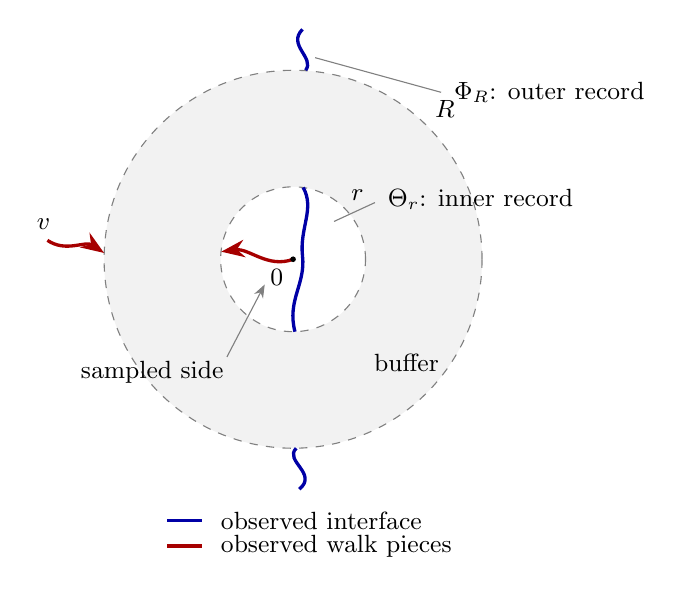
\begin{tikzpicture}[scale=.8,>=Stealth,font=\small]
  \fill[gray!10] (0,0) circle (3);
  \fill[white] (0,0) circle (1.15);
  \draw[dashed,gray] (0,0) circle (3);
  \draw[dashed,gray] (0,0) circle (1.15);
  \draw[very thick,blue!65!black]
    (.15,3.65) .. controls (-.1,3.4) and (.35,3.2) .. (.2,3);
  \draw[very thick,blue!65!black]
    (.1,-3.65) .. controls (.4,-3.4) and (-.15,-3.2) .. (.05,-3);
  \draw[very thick,blue!65!black]
    (.03,-1.15) .. controls (-.1,-.65) and (.2,-.4) .. (.15,.05)
    .. controls (.1,.5) and (.35,.8) .. (.16,1.14);
  \draw[very thick,red!65!black,->]
    (-3.9,.3) .. controls (-3.6,.1) and (-3.3,.3) .. (-3,.1);
  \draw[very thick,red!65!black,->]
    (0,0) .. controls (-.4,-.15) and (-.7,.18) .. (-1.14,.12);
  \fill (0,0) circle (.045);
  \node[below left] at (0,0) {\(0\)};
  \node[above left] at (-3.7,.32) {\(v\)};
  \node[anchor=west] at (1.35,.95) {\(\Theta_r\): inner record};
  \draw[gray] (1.3,.9)--(.65,.6);
  \node[anchor=west] at (2.4,2.65) {\(\Phi_R\): outer record};
  \draw[gray] (2.35,2.65)--(.35,3.2);
  \node at (1.8,-1.65) {buffer};
  \node[anchor=east] at (-.95,-1.8) {sampled side};
  \draw[gray,->] (-1.05,-1.55)--(-.45,-.4);
  \node[above right] at (.77,.77) {\(r\)};
  \node[above right] at (2.1,2.1) {\(R\)};
  \draw[very thick,blue!65!black] (-2,-4.15)--(-1.45,-4.15);
  \node[anchor=west] at (-1.3,-4.15) {observed interface};
  \draw[very thick,red!65!black] (-2,-4.55)--(-1.45,-4.55);
  \node[anchor=west] at (-1.3,-4.55) {observed walk pieces};
\end{tikzpicture}
\caption{The two records leave an annulus available for separation
and hookup. The inner walk arrow indicates reversal from the harmonic
landing. The shaded annulus is unexposed; no interface connection there
has yet been required.}
\label{fig:harmonic-records}
\end{figure}

\begin{lemma}[Hookup probability]\label{g:hookup}
For \(9R/8<R'<5R\), with the observer and exterior boundary outside
\(\mathfrak B_{6R}\), there is a universal upper bound for all
\(R\geq R_0\), where \(R_0>1\) is fixed:
\[
 \Prob(Z^\sigma\mid\Phi_{R'},\Theta_R)\leq C/\log R.
 \tag{G1}
\]
For every \(a>0\) there is \(c(a)>0\) such that the same probability
is at least \(c(a)/\log R\) when
\(Q(\Phi_{R'})\wedge Q(\Theta_R)\geq a\) and \(R\geq R_0(a)\).
\end{lemma}

\begin{proof}
The field part of \(\Phi_{R'}\) constrains only sites adjacent to
the external arms, hence outside radius \(R'-O(1)\).
The sites specifying \(\beta_R^\sigma\) lie inside radius \(R+O(1)\).
Choose comparison disks between these two radii, with
outer radius \((R+R')/2\) and inner radius \(R+(R'-R)/4\).
For sufficiently large \(R\), they have a free intervening annulus
of fixed relative width. The original base observations are all
outside the outer disk, and the external arms give the required
anchors. Thus Lemma~\ref{g:strand-comparison} applies to the two
orientations of the inner strand, comparing the exterior data with
their global sign reversal. Together with sign symmetry it gives a uniformly
positive probability that the two observed unoriented configurations
have compatible signs on the side containing the walk. In that case join corresponding interface tips and the two walk tips by
three polar centerlines.  We may assume \(a\le1/100\), since otherwise
the lower-bound hypothesis is empty.  After rounding their same-radius
angular gaps are at least \(a/2\).  Put
\(s=aR/(800\pi)\) and \(w=s/100\), reserve straight radial stems of
length \(20w\) at both ends, and interpolate the angles linearly between
the stems.  Since \(R'-R\ge R/8\) and \(40w\le R/(200000\pi)\),
the angular slopes are at most \(25\pi/R\).  At a common radius the
distance between centerlines is at least \(.49aR\).  If two radii differ
by at least \(s\), that gives the required separation directly; otherwise
moving along one centerline to the common radius costs at most
\((1+125\pi)s<.158aR\).  Thus the mutual separation is at least \(s\).
The observed external arms, the two free interface centerlines, and the
inner strand complete to one prospective simple oriented chord
\(\Gamma_0=K\cup J\), where \(K\) is the observed field system and
\(J\) its free completion.  The compatible orientation gives its two
sides \(\Omega_+\) and \(\Omega_-\).

Offset a lane by \(w\) on each side of each interface centerline.
At a tip the two offset lanes
meet its radius-\(4w\) circle at transverse offsets \(\pm w\) and
radial depth \(\sqrt{15}w\), up to bounded lattice error.  Follow from
the chosen lane the circular arc away from the radial stem.  The long arc
between the two lane points stays at distance at least \(w-O(1)\) from
\(J\); the other connector is farther by the centerline separation.
Its endpoints are on opposite ideal sides, so this arc must meet the old
boundary arc at that end.  At its start the full-boundary clearance is
greater than \(3w\), since the old record is on the old side of its
stopping circle and the other record is remote.  Stop at the first point
of full-boundary distance \(w/10\) and append a globally shortest segment
to \(b\in\partial D(K)\).  This segment remains in the selected side;
its endpoint is on the appropriate old pure bank, even if that bank
shadows the tip.  Moreover
\[
 \begin{aligned}
 d(b,J)&\ge .89w-O(1),\\
 d(b,\hbox{all observed tips})&\ge3.8w-O(1),\\
 d(b+tu,\partial D(K))&=t\quad(0\le t\le w/10).
 \end{aligned}
\]

Take \(d=w/(200A)\), with one fixed sufficiently large \(A\).  To check
the endpoint pocket, in each ideal side join free collars of the two
connectors \(J_1,J_2\) by the same-side arc on the middle-radius circle.
This arc is free and has macroscopic clearance, since the annulus has no
old observations.  Delete the triangles meeting \(K\) and use the
access-resolved component containing this connected reference set.  The
deleted triangles attach to its old boundary arcs, so its resolved
completion is a disk.  The radius-\(d\) crosscut met by the nearest
prefix misses the reference set.  The retained cap arc has clearance
\(w/10>d\), and a short transverse segment at its lane end reaches the
local radial stem with clearance greater than \(d\).  Thus the tail and
both connector collars are on the reference side of the crosscut.  The
other side is bounded by that crosscut and one pure old boundary arc,
and contains the initial nearest prefix.  This is the required pocket;
the prefix crosses each smaller circle once.  After the cap, a stem has
radial depth at least \(\sqrt{15}w\), and the interpolating portion is
at radial distance at least \(20w\) from either stopping layer before
the offset.  Subtracting the offset and curvature/lattice errors leaves
clearance greater than \(w/10\); the retained cap itself has that
clearance by its first-stop definition.  Choose the tube width so that its enlargements are
at most \(w/100\).
Use barrier scale \(\bar R=12R\). All four barriers lie in
\(B_{6R}\) and have radial span at least \(R/8-O(w)>d\), so their
diameters are less than \(\bar R\) and greater than \(d\). Thus
\[
       \theta=\frac{d}{\bar R}
              =\frac{a}{192\,000\,000\pi A}.
\]
The remaining lanes have clearance \(w/10\), so (UB1) holds with
clearance constant \(1/2\) after lattice error. The full endpoint
modules have radius
at most \(d+L\ell_c\le w/100\). Hence the sign-\(\pm\) confined
domains and prescription supports lie in \(\Omega_\pm\) and have
distance at least
\[
             w-w/10-w/100-w/100-O(1)\ge .85w
\]
from \(J\), including lattice error. A free path between opposite
sides cannot cross the fixed \(K\), so it must cross \(J\).
This verifies (UB2) at scale \(\bar R\) with
\(\kappa=.85w/(12R)>0\).
Proposition~\ref{g:barriers} applied to these four signed barriers
forces the interface joins within the disjoint corridors with
uniformly positive probability. Planarity forces the outer arms to
merge with the corresponding inner arms; there is no other exit
through the fences.

The remaining walk bridge must reach the joining vertex of the reversed
inner piece. Its conditioning to reach this vertex before zero has
probability bounded below. Harnack gives a positive probability to
follow the free third corridor to a fixed relative neighborhood of
that vertex; the two-dimensional point-hitting estimate gives
probability comparable to \(1/\log R\) to hit it there. The loop portion
between its first and last visits stays in that corridor with probability
bounded below, by the last-exit decomposition. This proves the lower
bound. Conditional on any completed field configuration, hitting the
same vertex before a nearby interface continuum has probability at
most \(C/\log R\); this proves the upper bound. These are precisely
the walk hypotheses of \cite[Lemma 3.14]{SSdiscrete}: radii in the
specified compact ratio range, observer outside the larger disk,
and two prescribed first/last walk pieces. All field estimates used
in its corridor construction have been supplied above.

We record the two augmented upper bounds used below. First, the upper
bound still holds after the whole field, hence \(\gamma\), is fixed;
the middle walk bridge remains unexposed. Second, put
\(H=(\Phi_{3r},\Theta_{2r})\), and expose that middle walk only until
its first exit from a circle of radius \(\rho/3>10r\), if this occurs
before its prescribed terminal piece. Call this stopped prefix
\(S_{**}\). On this escape event,
\[
 \Prob(Z^\sigma\mid H,S_{**},\hbox{escape})
       \leq C/\log r.                              \tag{GK}
\]
For verification, let \(\hat q\) be the joining vertex of the fixed
reversed inner piece. The first-hit/last-exit decomposition leaves a
walk from the current exit vertex to \(\hat q\), conditioned to hit
\(\hat q\) before zero, followed by its last-exit loop. Harnack bounds
the conditioning probability below by a fixed constant, since the
exit vertex is outside \(B_{10r}\) while
\(|\hat q|=2r+O(1)\). To realize \(Z^\sigma\), this first part
must hit \(\hat q\) before the connected inner interface. The same
point-versus-continuum estimate as above is at most \(C/\log r\);
the remaining loop can only reduce the probability. This argument
holds for every completed field consistent with the records, and
averaging gives (GK). It does not expose the later successful bridge.
\end{proof}

\begin{lemma}[Separation under a harmonic landing]\label{g:separation}
For every \(\eps>0\) there is \(c(\eps)>0\) such that, for all
sufficiently large \(R\),
\[
 \Prob\bigl(Q(\Phi_{3R})\wedge Q(\Theta_{2R})>c(\eps)
       \mid\Phi_{4R},\Theta_R,Z^\sigma\bigr)>1-\eps .       \tag{G2}
\]
The estimate is uniform in admissible records for which the conditioning
has positive probability.  The observer and original boundary are outside
\(\mathfrak B_{12R}\).
\end{lemma}

\begin{proof}
Write \({\cal F}_{r,s}=\sigma(\Phi_r,\Theta_s)\), and write
\(\widehat q_{\rm o},\widehat q_{\rm i}\) for the two numerical quality
formulas above, before the following common live test.  An exact pair is
called open if both pairs of strand tips exist, neither observed interface
has closed or prematurely merged, and the observed walk has made no
forbidden contact with any observed strand or with the original exterior;
the prescribed terminal contact at zero is the sole exception.  The raw
qualities are zero if these conditions fail.  A pair is called live when
\(\Prob(Z^\sigma\mid{\cal F}_{r,s})>0\); its two qualities are the raw
qualities when live and are set to zero otherwise.  A live pair is open.
We shall update only one of the two records at a time.
For the outer record put \(\rho=r\) and \(e=-1\), and for the inner
record put \(\rho=s\) and \(e=1\).  If the selected record has quality
\(q>0\), put
\[
       L=q\rho,\qquad \rho_1=(1+10eq)\rho .
\]
Let \(q_1\) denote its quality after this update, including the live-pair
test, with the other record held fixed.  We first prove, uniformly for
\[
 3.3R<r\le4R,\qquad R\le s<1.7R,\qquad
 0<L<R/200,\qquad L\le\rho_{\rm other}q_{\rm other},
\]
where \(\rho_{\rm other}\) and \(q_{\rm other}\) are the radius and
live quality of the unchanged record,
that
\[
 \Prob\bigl(q_1\ge2q\mid{\cal F}_{r,s}\bigr)\ge c_0>0.
                                                               \tag{G3}
\]
Here \(q=L/\rho<1/200\), so the cap is inactive.  The geometric,
barrier, and walk construction will be proved in the wider layout buffer
\[
 2.8R<r\le4R,\qquad R\le s<1.84R,\qquad
 0<\widehat q\le1/100,
\]
for any jointly admissible open pair, using its selected raw quality
\(\widehat q\), again denoted by \(q\) there.  Only the positive-support
step will use the smaller-
physical-separation premise in (G3).
For the low-quality updates used later we also prove the following joint
form.  Put \(F=\{q_1<2q\}\), and, on \(F\cap\{q_1>0\}\), make one
further update of the same record to
\(\rho_2=(1+10e q_1)\rho_1\), leaving the other record fixed.  Put
\(q_2=0\) on \(\{q_1=0\}\).  If \(q<1/500\), \(r>3.25R\), and
\(s<1.61R\), then
\[
 \Prob(F,q_2=0\mid{\cal F}_{r,s})
       \ge c_1\Prob(F\mid{\cal F}_{r,s}).                    \tag{G4}
\]
Both subsequent radii in (G4) remain in the wider layout buffer just
displayed.
The estimates condition on the stopped records, not on \(Z^\sigma\).

\paragraph{The three local centerlines.}
The selected two strand tips and walk tip have pairwise distance at least
\(L\).  Each strand tip has distance at least \(L\) from the entire old
walk, and the walk tip has distance at least \(L\) from the entire old
strand.  All those histories are on the old side of the rounded circle.
Their deviation from the Euclidean circle is bounded by a lattice constant
\(c_\triangle\).  Below, fixed errors \(O(c_\triangle)\) include the
short access from an actual tip to a circular polar coordinate.  Such
accesses can be chosen in the unobserved side: for an outer tip use the
interior of an incident selected hexagon to reach the Euclidean circle;
for an inner tip use the unselected-hexagon construction given below.

Cut the cyclic order of the three access angles at a largest gap and lift
them to \(a_1<a_2<a_3<a_1+2\pi\).  Write
\(g_i=a_{i+1}-a_i\) for \(i=1,2\) and
\(g_3=2\pi-a_3+a_1\ge2\pi/3\).  Define
\[
 \delta_i=(5q-g_i)_+,\qquad
 (\Delta_1,\Delta_2,\Delta_3)
  =\tfrac12(-\delta_1-\delta_2,\ \delta_1-\delta_2,
                         \ \delta_1+\delta_2).                 \tag{G3a}
\]
Use a fixed tie rule in choosing the cut.  Then \(|\Delta_i|\le5q\).
During interpolation by a parameter \(t\in[0,1]\), the first two gaps
are \(g_i+t\delta_i\); the cut gap is
\(g_3-t(\delta_1+delta_2)\ge2\pi/3-10q>1.99\).
Thus the cyclic order is preserved, no already larger gap is reduced
except the largest one, and all three final circular gaps are at least
\(5q\).

For the moment suppose \(L\ge L_0\), where the fixed threshold \(L_0\)
will absorb all lattice errors.  From the short circular access, retain
a straight radial stem of length \(L/10\).  Spread the angles linearly
to \(a_i+\Delta_i\) by radial progress \(5L\), and keep these angles
fixed for the final radial progress \(5L\), ending at radius \(\rho_1\).
Continue the held rays to total radial progress \(11L\) for the barriers
and to total progress \(13L\) only for a topological completion.  The
spread width is \(4.9L+O(c_\triangle)\).  During spreading the radii
stay between \(.95\rho\) and \(1.05\rho\); using the conservative
factor \(1.1\), after increasing \(L_0\) the ratio of arclength speed
to radial speed is at most
\[
             v_* =\sqrt{1+(5.5/4.89)^2}<1.51.                 \tag{G3b}
\]
The total length of a barrier, including its held extension and the
endpoint construction below, is at most
\(11L+5.5L+O(L/2000)+O(c_\triangle)<17L\).

Here are the required uniform separation estimates.  For \(L_0\) large,
the circular access gaps are at least \(.98q\).  Even through total
progress \(13L\), the common radius is at least \(.87\rho-O(c_\triangle)\).
The corresponding centerline points have distance at least
\(2(.87\rho-O(c_\triangle))\sin(.49q)>.84L\).
If two points have radial difference at least \(L/4\), their distance
has that lower bound.  Otherwise compare at a common radius and use
(G3b), losing less than \(1.51L/4\); the remainder exceeds \(L/4\).
The same argument applies to a stem, a spread piece, or a held extension.
For a short access piece, use its bounded length and the following
old-side estimate.  If \(H\) is an opposite old history and a centerline
point has radial progress \(u\), then
\[
 d(z,H)\ge\max\{L-v_*u-O(c_\triangle),\ u-O(c_\triangle)\}
       \ge {L\over1+v_*}-O(c_\triangle)>.38L.                \tag{G3c}
\]
This also proves the distance from each complete local centerline to the
entire opposite old history.  Consequently any two complete centerlines
are separated by \(L/4\), after one further increase of \(L_0\).

Let \(t_i\) be the three target points at radius \(\rho_1\).  Every
piece of a different centerline before the held part is radially at least
\(5L-O(c_\triangle)\) from \(t_i\).  The distance from \(t_i\) to any
ray whose circular angular distance is at least \(5q\) is at least
\(\rho_1\sin(5q)\): for an angle at least \(\pi/2\) the lower bound
is \(\rho_1\), and otherwise it is the perpendicular distance to the
infinite ray.  This covers the entire held piece and its extension.
Since \(\rho_1\le1.1\rho\) and \(q\le.01\), it follows that
\[
 d(t_i,\hbox{the entire other centerline})
       \ge4.4q\rho_1.                                      \tag{G3d}
\]
This bound includes the bounded access errors.  It is the final held
length \(5L\), rather than only the final angular gap, which controls
the earlier spreading portions.

\paragraph{Four barriers with fixed parameters.}
Put \(w=L/2000\), \(\ell=w/10\), and \(d=w/(200A)\), where \(A\)
is a sufficiently large fixed constant.  Smooth the two centerline
corners in \(O(w)\) neighborhoods, preserving the initial radial stem,
radial monotonicity, and all preceding estimates with a small fixed loss.
The two sides of a regular radius-\(w\) tube about each strand centerline
give its two side lanes.  Such a tube is a strip: the stem and held pieces
are radial, the middle piece is a graph over radius with slope bounded
by (G3b), and the two corners can be rounded with curvature at most
\(1/(10w)\).  The strips for distinct centerlines are disjoint.

For an outer update, complete only the two outer observed arms by these
two centerlines and a simple connector at radial progress \(13L\).
This is a prospective oriented chord \(K_{\rm o}\cup J\).  For an inner
update, use the inner observed strand and the two outward centerlines,
joining at radial progress \(13L\), to obtain a prospective oriented
simple loop.  Let \(K_0\) be the selected old field system, and denote
the two ideal sign sides of \(K_0\cup J\) by \(\Omega_+\) and
\(\Omega_-\).  They are Jordan disks, with the unbounded side of an
inner loop viewed on the sphere.  For an actual attachment in side \(s\),
delete from \(\Omega_s\) the closed lattice triangles meeting \(K_0\), take the component
incident to the connected free collar of \(J\), and take its prime-end
completion.  The deleted triangles attach to the \(K_0\) boundary, so this
component has connected complement and its resolved completion is a disk.
Its non-\(J\) boundary incidences away from tips and marks are the pure
sign-\(s\) bank.  This is the attachment side; a raw pinched component of
\(D(K)\) is not being called a Jordan disk.  The connector is only a
topological separator; no rectangle,
shift, or barrier follows it.  It stays at least \(2L-O(w)\) beyond the
barrier endpoints.  The other stopped field record is disjoint from the
completion because
\[
  (1-13q)r\ge.87(2.8R)>1.84R,\qquad
  (1+13q)s\le1.13(1.84R)<2.8R.                              \tag{G3e}
\]
No compatibility of the sampled inner orientation is assumed here.

We spell out the old-end attachment; it also handles a shadowing return
of the other old arm.  At an actual tip take the circle of radius \(4w\).
The two side lanes meet it at transverse offsets \(\pm w\) and radial
depth \(\sqrt{15}w\), up to \(O(c_\triangle)\).  Follow the circle from
the chosen lane away from the radial stem.  The long arc between these
two lane points stays at distance at least \(w-O(c_\triangle)\) from
the local \(J\); the rest of \(J\) is farther by the stem length and
the centerline separation.  The two lane points are on different sides
of \(K_{\rm o}\cup J\), or of the inner loop.  Thus this arc, which
avoids \(J\), must hit the old field boundary.  At its starting point
the full-boundary clearance exceeds \(3w\): the old record is on the
old side of the rounded circle, and the curvature error is
\(O(w^2/\rho)+O(c_\triangle)=o(w)\).  Stop at its first point \(a\)
of full-boundary distance \(\ell\), and append a globally shortest
segment from \(a\) to \(b\in\partial D(K)\).  The retained circular
arc has clearance at least \(\ell\).  The segment cannot cross \(J\),
since its length is \(\ell<w-O(c_\triangle)\), and it cannot cross a
different fixed boundary before its endpoint.  It is therefore in the
chosen actual side.  Its endpoint lies on an old string, not on the
remote record or exterior, and
\[
 d(b,J)\ge .89w-O(c_\triangle),\qquad
 d(b,\hbox{every observed tip})\ge3.8w-O(c_\triangle).       \tag{G3f}
\]
For later caging, identify this actual endpoint with the ideal bank as
follows.  In the incident deleted triangle selected by its nearest prefix
and meeting \(K_0\), join \(b\) to the first \(K_0\)-hit.  The link has
diameter at most one and stays in the signed ideal side by (G3f).  It is
only an identification through forbidden material, inaccessible to a new
dual continuation away from an active strand tip.  Coincident links are retained as
separate incidences in their boundary order.  This link is not a free path
and is not used to prove the pocket.

The nearest segment has exact clearance
\(d(b+tu,\partial D(K))=t\) for \(0\le t\le\ell\).

This attachment has the pure pocket required by Proposition~\ref{g:barriers}.
Take the radius-\(d\) circular crosscut in the resolved attachment side which
the nearest segment meets.  The circle misses \(J\) by (G3f), so its
two boundary incidences are on the pure bank.  The retained circular arc
has distance at least \(\ell>d\) from \(b\).  From its lane endpoint a
short transverse segment reaches the radial stem at depth about \(4w\);
this segment also has full-boundary clearance greater than \(d\).
It follows that the tail and a collar of \(J\) are on the same side of
the crosscut, while the initial nearest prefix is on the other side.
The crosscut theorem in the Jordan side makes that latter component a
pocket bounded by the crosscut and the single pure boundary subarc which
excludes \(J\).  The nearest prefix crosses every smaller circle once.
The remote record is on the \(J\)-side: in the outer case it lies in
the connected region below radius \(r-L/20\), and in the inner case
in the region above radius \(s+L/20\); these regions reach the stem and
miss the radius-\(d\) crosscut.  Removing the remote record cannot
alter the pocket.  This proof does not assert that the pure subarc or
the pocket has small diameter.

After deleting only the nearest prefix of length \(3d/5\), its remainder
has clearance at least \(3d/5\); the retained circular arc and lanes
have clearance at least \(\ell\), and the free endpoint is remote from
all pins.  Thus (UB1) holds with \(a=1/2\), including the bounded lattice
error.  A point within \(d/5\) of the boundary lies on the nearest prefix
at radius less than \(d/2\), proving the ordinary near-boundary barrier
condition as well.  The endpoint testing window is \(B(b,O(d))\).
Every component of an old simple strand cut by its generous testing
square meets the rim, since all strand tips and the remote record are
outside that square by (G3f).  The incident component also reaches the
rim.  This proves local thickness, even with arbitrarily many returns.
All tested pure pins and the traced pin chain are string pins: these
windows are near radius at most \(4R\), whereas the original exterior
is outside \(12R\).  A remote pure subarc may traverse exterior, but
no exterior pin enters the quantitative attachment estimate; its constant
is the interior-string constant of Proposition~\ref{g:barriers}.

Use the four side barriers only through radial progress \(11L\).
Their radial span exceeds \(d\), and their diameters are less than
\(17L\).  Take common barrier scale \(\bar R=32L\).  Choose the fixed
mesh and interpolation neighborhoods in the proposition so that every
full endpoint module has radius at most \(w/100\) and every tube
enlargement has width at most \(w/100\).  The full domains \(C_\pm\)
and all supports \(P_\pm\) lie in their corresponding \(\Omega_\pm\)
at distance at least \(.8w\) from \(J\), by the lane offset, (G3f), and
the two \(w/100\) losses.  A free path between opposite sides cannot
traverse fixed \(K\), hence must cross \(J\).  This proves (UB2).
For the ordinary internal distance, an access-labelled admissible path
has its interior in \(U\).  Under the preceding forbidden-material bank
identifications it starts on opposite ideal sides of the continuous
separator \(K_0\cup J\); it cannot meet \(K_0\), and therefore crosses
\(J\cap U\).  Its diameter is at least \(.8w>2d\).  Thus the ordinary
opposite-barrier separation also holds, with the fixed choices
\[
 \theta={d\over32L}={1\over12\,800\,000A},\qquad
 m=4,\quad a=1/2,\quad \kappa={.8w\over32L}={1\over80\,000}.   \tag{G3g}
\]
The observed component near an endpoint supplies the required anchor.
There are a bounded number of smooth pieces and turns, and all rectangle
counts in the proposition depend only on (G3g), not on \(q\).  The
probability of avoiding all four barriers is therefore at least a fixed
\(p_{\rm b}>0\) under either actual inner orientation.

\paragraph{What the barriers force.}
Add only for topology a transverse gate from each side barrier's free
endpoint to the corresponding centerline at radial progress \(11L\).
The two gates for tip \(i\) end at the same point \(g_i\in J\), beyond
the stopping circle.  In the ideal \(\Omega_s\), adjoin the forbidden-
material endpoint link; the side barrier plus this link and gate is a proper
crosscut \(A_{i,s}\) from the pure bank \(B_s\) to \(J\).
The two same-sign crosscuts are disjoint.  Parametrize \(B_s\) and \(J\)
from tip 1 to tip 2.  Their \(J\)-endpoints have this order, so their
\(B_s\)-endpoints have the same order: otherwise the four endpoints
alternate and the crosscuts must meet.  This conclusion permits both
attachments to be on shadowing parts of the old strand.

Glue the two Jordan sides along \(J\), retaining distinct incidences
on the two fixed banks.  The union \(Y_i=A_{i,+}\cup A_{i,-}\) is a
proper crosscut in this split-bank domain.  The preceding nonalternation
gives disjoint tip-1 and tip-2 end components and a central component.
Extra fixed observations can only remove points.  In the relative boundary
of an end component the two virtual \(J\) portions cancel; its only exits
are actual barriers, fixed boundary, and its beyond-stop gates.  A fresh
interface prefix which avoids the barriers and is stopped at the new
circle therefore stays in its end component.  The two prefixes cannot
merge there.  For an outer update the completed chord must connect the two
old tips; for an inner update the complete component either joins the two
continuations or reaches the original exterior, which is beyond the new
circle.  Thus neither case can lose a target tip before the stopping circle.
On the new circle all cap and turning pieces are behind,
and each held lane crosses in one bounded lattice block.  The end component
meets that circle precisely in the short interval between its two lane
blocks.  Each new strand tip is consequently within \(O(w+c_\triangle)\)
of its target.  No metric confinement of the rest of that prefix in a
narrow tube is asserted.

Put \(\nu=L/1000\).  Require the fresh walk to follow the width-\(\nu\)
tube about its centerline through a terminal extension of length \(2\nu\),
including a full entrance ball of radius \(L/100\) about its starting
vertex and the radius-\(\nu\) terminal ball.  The terminal ball extends
at least \(\nu\) beyond the new circle.  The entire corridor meets that
circle only within \(\nu+O(c_\triangle)\) of the target: the entrance ball
is \(10L\) away, the spreading pieces are at least \(5L\) away, and the
remaining tube follows the held ray.  Stop the successful walk at its first
crossing of the new rounded circle in this window.  The
entrance ball is not clipped at the old circle and may meet the old walk.
By (G3c) it misses the old field, and centerline separation makes the
whole tube and ball miss the side barriers and their gates, including the
hexagon error.  They lie in \(B_{5R}\), so they also miss the original
exterior outside \(\mathfrak B_{12R}\).  Let \(X\) be the ideal ambient
disk or sphere slit only along the selected old dual system \(K_0\), with
its bank accesses retained and the short forbidden endpoint links included
in \(Y_1\cup Y_2\).  Let \(W\) be the union of the closed hexagons of
every old and fresh visited walk vertex, not just the polygonal walk edges.
Every cell interior avoids \(K_0\), which lies on hexagon edges.
Consecutive visited cells share an edge not crossed by \(K_0\): for the
old record this is the open no-prior-contact condition, including the
reversed first step from zero, since otherwise its forward predecessor
would already be adjacent to the interface; for the fresh part it is the
tube clearance.  Thus \(W\setminus K_0\) has a connected lift to \(X\),
with the prescribed access along the old contacts of the origin cell.
Those boundary contacts are not asserted to be in the open surface.
The old walk misses the crosscuts because away from the \(O(w)\) tip caps
they lie on the new side of the old circle, while the old quality protects
the caps.  Together with the tube separation, this makes \(W\) disjoint
from \(Y_1\cup Y_2\), including their links and gates, after the hexagon
error.  The terminal cell meets the central circle interval.  Hence the
connected lift of \(W\setminus K_0\) lies in the central component of
\(X\setminus(Y_1\cup Y_2)\), even if it crosses virtual \(J\).  A fresh
dual prefix stays in an end component, so it cannot meet \(W\) off
\(K_0\).  It cannot newly enter \(K_0\) away from an active strand tip; the
pre-existing origin contact remains allowed.

Put a ball about the deterministic walk target of radius
\(2q\rho_1+\nu+O(c_\triangle)\), including the full landing-window
and hexagon errors.  Equations (G3c)--(G3d), the \(5L\) radial hold,
and the \(O(w)\) gates show that this ball misses both paired crosscuts
\(Y_i\).  It also misses the old field by the \(10L\) radial gap.
It misses the remote stopped record by (G3e), including this ball radius.
The ball is connected and contains the central target; its lift to the
split-bank domain is wholly central even if it crosses virtual \(J\).
Thus the actual walk tip is at distance at least \(2q\rho_1\) from the
entire newly observed field.  Conversely each new field tip is within
\(O(w+c_\triangle)\) of its target; (G3d) bounds its distance to the
entire new walk tube, and the radial gap bounds its distance to the entire
old walk.  Both exceed \(2q\rho_1\).  Finally the two field targets have
distance at least \(2\rho_1\sin(5q/2)\), which still exceeds
\(2q\rho_1\) after the landing errors.  Hence every term in the new
quality numerator is at least \(2q\rho_1\), and no forbidden contact
or premature merger has occurred.

\paragraph{The walk probability.}
For \(x,y\ne0\), put
\[
 G_0(x,y)=\sum_{n\ge0}\Prob_x(S_n=y,\ n<T_0).
\]
This killed Green function is finite and symmetric.  If the exact outer
and reversed inner walk records end at \(a\) and \(b\), the unexposed
middle path has law
\[
 \mathsf B_{a,b}(m)={6^{-|m|}\over G_0(a,b)},\qquad
 m:a\longrightarrow b,\quad m\cap\{0\}=\varnothing.          \tag{GW1}
\]
The fixed prefix and suffix contribute a common factor to the walk weight;
summing the remaining weights gives \(G_0(a,b)\).  All revisits of either
recorded history or circle are permitted.  Reversal is exactly
\(\mathsf B_{b,a}\), including all loops, and the field record does not
change this law before conditioning on \(Z^\sigma\).

Let \(E\) be the successful entire-corridor first-crossing event specified
above, stopped at \(\tau\).  Summing the still unexposed remainder in
(GW1) gives for an outer extension
\[
 \mathsf B_{a,b}(E)
       ={\E_a[\mathbf1_EG_0(S_\tau,b)]\over G_0(a,b)}.       \tag{GW2}
\]
The full entrance ball and width-\(\nu\) tube have length \(O(L)\) and
are covered by a fixed number of overlapping balls of radius comparable
to \(L\).  Their entire corridor and a fixed relative enlargement containing
the doubled Harnack balls stay between radii \(.89r\) and \(1.01r\) for
an outer update, or between \(.99s\) and \(1.12s\) for an inner update.
The remote-pole gaps are bounded below by
\[
 .89(2.8R)-1.84R>.65R,\qquad
 2.8R-1.12(1.84R)>.73R,
\]
and the enlargement is also a fixed positive distance from zero.  Since
\(L\le.04R\), these are uniform relative Harnack margins.  Ordinary
walk traverses the ball chain with a fixed positive probability.  Positive
harmonicity of \(G_0(\cdot,b)\) on its doubled balls compares its value
on the landing window with \(G_0(a,b)\), so (GW2) is at least a fixed
\(p_{\rm w}>0\).  The full entrance ball permits the necessary old-circle
recrossings.  After any exact outer prefix ending at \(a'\), the remaining
law is \(\mathsf B_{a',b}\); reversing it gives the inner estimate with
\(G_0(\cdot,a')\).  The current stopped layers remain strictly nested,
and the same displayed pole margins hold for every current joining vertex
in the buffer.  Thus this also applies after an earlier one-record update,
without an independence assertion.  Field and walk are independent given
their respective stopped records and the actual field orientation.  The
bound \(p_{\rm b}p_{\rm w}\) survives averaging over that orientation,
and gives an open raw output of quality at least
\((2q)\wedge1/100\) with this uniform probability for \(L\ge L_0\).
This part has not used the live test.

\paragraph{Bounded lattice scales.}
We use a simultaneous form of bounded insertion.  Given a fixed number
\(m\) of fixed-size patches near observed tips and compatible sign
prescriptions on a bounded number of their free vertices, their joint
probability under the original exact-strand conditioning has a positive
uniform lower bound.  Fix first the shell failure parameter \(1/(4m)\).
For each fixed patch size choose the corresponding long-slack enlargement
from the proof of Lemma~\ref{g:insertion}, with this parameter and its
required deficit.  Merge clusters whenever their already chosen enlarged
boxes, with one neighbor layer, intersect, recomputing the enclosing box
with the same parameter after a merge.  There are at most \(m-1\) merges,
and overlap bounds each new diameter by a deterministic function of the
previous ones.  Thus the final boxes have uniformly bounded sizes and no
edges between their interiors; there is no later enlargement.  The arbitrary
animal parameter in Corollary~\ref{f:conditioned-sparse} makes each shell
failure less than \(1/(4m)\).  With probability at least \(3/4\) all
shells are good.  Construct the prescribed feasible filling separately
inside every box, keeping all shells fixed.  On their disjoint interiors
perform one joint contraction toward these fillings.  Its Jacobian is
\(t^{\sum N_i}\), with \(t>0\) and \(\sum N_i\) bounded by the patch
parameters.  Integrating proves the joint bound.  No first fence pattern
is used as a new conditioning for a second invocation.

For \(L\le20\) use the deterministic triangular/hexagonal routing in
\cite[proof of Lemma~3.15, pp.~65--66]{SSdiscrete}.  It uses only the
local rounded-circle geometry, the full-history quality inequalities,
and positive completion support.  Its longest boundary arc and extremal
left/right dual continuations leave a bounded primal route avoiding all
adjacent hexagons, with doubled quality and preserved completion support.
The same construction with first exit in place of first entry gives the
inner route; the fixed ratio \(r/s>1.52\) keeps the opposite record out
of its bounded patches.  The simultaneous insertion argument just proved
replaces only the field probability input.  A prescribed primal route of
at most \(M\) steps has, under either Green transform in (GW2), probability
at least \(6^{-2M}\): for the current remote pole \(b\), harmonicity gives
\(G_0(v_{j+1},b)\ge G_0(v_j,b)/6\) at each step.  Thus this branch has a uniform
positive probability without drawing sublattice-width barriers.

For \(20<L<L_0\) we give a direct finite construction.  Put
\(h_{\mathrm{hex}}=1/\sqrt3\).  For an outer strand tip, join it through an
incident selected hexagon to a point of the Euclidean radius-\(r\) circle;
this costs at most \(2h_{\mathrm{hex}}\) and avoids the old dual strand.  For
an inner tip choose an incident unselected hexagon with center \(v\),
join the tip to \(v\) through its interior, and choose a lattice unit
vector \(e_v\) with \(e_v\cdot v/|v|\ge\sqrt3/2\).  An unselected
hexagon has \(|v|\ge s+1/2\), since it contains the radius-\(1/2\) disk
about its center, and boundary incidence gives \(|v|\le s+3h_{\mathrm{hex}}\).
For every integer \(k\ge1\),
\[
 |v+ke_v|\ge |v|+k\sqrt3/2>s+h_{\mathrm{hex}},
\]
so these successive hexagons are unselected.  Their center segments
remain in the unselected union.  Follow them until the radius-\(s+7/4\)
circle is first met.  This occurs after center-path length at most
\((7/4-1/2)/(\sqrt3/2)<1.444\); the whole tip access has length less
than \(2.022\) and avoids the inner strand.  Use the radial circular
access for the walk, with its bounded first-entry or first-exit error.

The outer access points have pair distance at least
\(L-4/\sqrt3>.88L\).  Use (G3a) with its signed shifts bounded by
\(4.12q\), an initial radial prefix to radius \(r-8\), spreading to
\(r-5L\), and the final held piece to \(r-10L\).  The spread width is
at least \(4.6L\).  Comparing spread parameters at threshold \(1/12\)
gives either radial separation \(4.6L/12>.383L\), or angular gap at
least \((.88-4.12/12)q>.536q\), whose chord exceeds \(.50L\).
The same comparison handles a prefix against a spread or held piece.
The short access pieces have length at most \(2/\sqrt3\) and stay within
a bounded vanishing radial sagitta of the old circle.  Against another
prefix, either their radial gap is at least \(7.7\), or that prefix is
within \(2/\sqrt3+7.7+o(1)\) of its own tip; the original separation then
leaves more than \(20-4/\sqrt3-7.7-o(1)>9.9\).  Against a spread piece
the radial gap is at least \(8-o(1)>7.66\), and held pieces are farther.
Thus the outer complete centerlines have mutual distance \(>7.66\).
Their speed ratio is at most \(\sqrt{1+(4.12/4.6)^2}<1.35\), so the
outer analogue of (G3c), with old histories outside radius \(r-1\), is
\[
 d(z,H)\ge\max\{L-2/\sqrt3-1.35u,\ u-1\}>.36L>7.2.       \tag{G3i}
\]

For the inner access circle the pair distance is at least
\(L-4.044>.797L\); since \(s\ge2000\), its angular gaps are at least
\(.796q\).  The centered shifts in (G3a) are at most \(4.204q\).
Take the straight prefix to radius \(s+10\), spread to \(s+5L\), and
hold to \(s+10L\).  The spread width is at least \(4.5L\).  At parameter
threshold \(1/11\), the two alternatives give radial separation
\(4.5L/11>.409L\) or angular gap
\((.796-4.204/11)q>.413q\), whose chord exceeds \(.412L\).
A short access has radius at most \(s+7/4\), whereas a spread piece has
radius at least \(s+10\), giving gap \(8.25\).  Against another prefix,
either the radial gap is at least \(7.8\), or that prefix is within
\(2.022+7.8\) of its own tip; the original tip separation then leaves
more than \(20-2.022-(2.022+7.8)>8.15\).  Hence all inner complete
centerlines have mutual distance greater than \(7.8\).  The old inner
strand is inside radius \(s+2/\sqrt3\) and the whole old reversed walk
inside radius \(s+1+1/\sqrt3\).  The speed ratio after the access is
less than \(1.41\).  The counterpart of (G3c) is therefore greater
than \(7.5\) for \(L\ge20\); explicitly, for radial depth \(u\ge7/4\),
it is at least
\[
 \max\{L-2.022-1.41(u-7/4),\ u-1-1/\sqrt3\}>7.5.          \tag{G3j}
\]
The short access itself has distance at least \(L-2.022\) from the
opposite old history.

Use finite side lanes of width \(w_b=3\) and first full-boundary stop
distance \(\ell_b=4/3\).  Near a tip take the appropriate one-sided
outer boundary of the radius-three neighborhood of its short access and
straight prefix, truncated at outer depth six or inner depth eight.  The
short access has diameter less than three, so its radius-three disks have
a common interior core; adjoining the monotone radial prefix gives a local
strip with an end cap.  Its side frontier has distance three from the local
\(J\).  The future spread starts two radial units farther.  Its tangential
slope is at most \(.982\), so even in the direction of the offset point its
distance there is at least
\(\min_{t\ge0}\sqrt{(2+t)^2+(3-.982t)_+^2}>3.5\), up to a vanishing
polar-curvature error; earlier points of the end collar are farther.
Other centerlines are farther than \(7.66\).  Thus this local frontier
has distance three from the full \(J\), and it joins the side boundary of
the full radius-three tube.  Its deep point has full deleted-boundary
clearance greater than \(6-1-o(1)>4\) in the outer case and
\(8-2/\sqrt3-1-o(1)>5.8\) in the inner case.

The old strand must meet this frontier near the tip.  For the outer case take its first point at
distance ten from the tip.  A \(J\)-point of inward depth at least four
is at least four from the old strand; a shallower one is within
\(4+2/\sqrt3<5.16\) of its own tip, giving distance greater than
\(10-5.16>3\) from that old point, for either local \(J\).
For the inner case a \(J\)-point of outward depth at least five is at
least \(5-2/\sqrt3>3\) from the old strand; a shallower one is within
\(2.022+(5-7/4)<5.273\) of its own tip, again leaving distance greater
than \(10-5.273>3\).  These old points exist because the relevant old
strand continues a macroscopic distance to the exterior or to the
incident-edge neighborhood.  Its arc starts on \(J\) and exits the
radius-three neighborhood.  It cannot exit through the deep cross-section,
which is strictly on the new side of the old radial bound.  In each actual
Jordan side the local strip frontier from the deep lane must therefore end
on the old boundary; an earlier shadowing return only ends it sooner.
Stop at the first clearance
\(\ell_b\) and nearest-attach.  Every point of this open finite barrier
then has distance at least
\[
                  3-4/3=5/3>2/\sqrt3                       \tag{G3k}
\]
from \(J\).  Continue along the held lane to a free endpoint beyond the
new circle and add the same virtual gate as above.

To identify the actual endpoint \(b\in\partial D(K)\) with its bank of
the central chord or loop, choose the incident deleted triangle which
meets \(K\), and join \(b\) inside that triangle to its first \(K\)-hit.
The triangle has diameter one, less than \(d(b,J)\ge5/3\), so this link
stays on the same bank.  It is only an identification inside forbidden
material, not a free path or a sign prescription.  Coincident links are
resolved in their boundary order.  An actual dual continuation cannot use
such a link or enter its endpoint away from an observed tip.

Perturb these finitely long barriers off dual vertices.  Prescribe sign
\(s\) at every free primal vertex whose closed hexagon meets an open
sign-\(s\) barrier.  An already fixed hexagon meeting it has sign \(s\):
its interior lies on that bank of the prospective chord or loop, and by
(G3k) it cannot also meet \(J\).  Remote fixed observations miss these
bounded lanes.  No free hexagon meets opposite-sign barriers, for a path
through that hexagon between the two sides would have to cross \(J\),
requiring diameter at least \(5/3\), greater than the hexagon diameter.
These are compatible prescriptions on at most \(M(L_0)\) vertices in
at most two bounded patches near the old tips.  The simultaneous insertion
argument gives them a joint positive probability.  At a transverse crossing
of an open barrier, both hexagons adjacent to the crossed dual edge meet
that barrier and have its strict sign.  A zero interface cannot cross it,
nor pass through its fixed endpoint away from a tip.  The paired-crosscut
caging proof above therefore applies literally.

For the walk, the cells successively met by its centerline give a primal
nearest-neighbor route in its full radius-one tube; at a cell-vertex tie
insert an incident neighboring cell.  Include the full radius-one entrance
ball and extend the route two units beyond the target circle.  In the inner
case the final crossed cell center has radius at least
\(s+10L+2-1/\sqrt3>s+10L+1/\sqrt3\), so it is unselected and the route
has exited.  Stop at first exit; use first entry in the outer case.  The
route has at most \(M(L_0)\) steps and controls the whole new walk history,
including revisits.  The fixed radial buffer keeps every route vertex away
from zero and stops it before the remote joining vertex.  Equations
(G3i)--(G3j) and the centerline separations
leave fixed lattice room between this tube and the finite sign fences.
The new field tips lie within five lattice units of their targets.  The
targets are at radial distance \(5L\) from all earlier pieces and at
distance at least \(4.8q\rho_1\) from every other held ray; subtracting
the target, lane, and hexagon errors (at most eight units) still leaves
more than \(2q\rho_1\) for \(L>20\).  Old histories are separated by
the \(10L-O(1)\) radial gap.  The expanded target-ball and central-
component argument controls the entire fresh field, as before.  The
finite route probability is at least \(6^{-2M(L_0)}\) by (GW2).
Thus the direct construction gives an open raw output of quality at least
\((2q)\wedge1/100\) with a uniform positive probability on the remaining
bounded range, before the live test.  The same deterministic construction
works with any fixed upper bound in place of \(L_0\); only the finite
cell count and its probability constant change.

\paragraph{Positive support after direct steering.}
The branch \(L\le20\) already includes the completion support in its
cited discrete routing conclusion.  Suppose now that \(L>20\) in (G3),
and fix any exact output pair in the successful open raw event just
constructed.  The unchanged physical separation is at least \(L\), by
the hypothesis of (G3), and the updated one is at least
\(2(1-10q)L>1.9L\).  Thus both raw physical separations exceed twenty.
The input live pair has a compatible cyclic matching of its two strand
accesses and its walk access, obtained from any completion witnessing
\(Z^\sigma\).  The target order and the landing error bounds show that
direct steering preserves this matching.  It is a geometric matching;
the inner orientation sampled for the raw event is not retained.

Fix a sufficiently large absolute \(H\), to be specified below.  From
the fixed output pair prospectively update any raw physical separation
\(\ell<H\), leaving the other record fixed, until both are at least
\(H\).  Use the direct finite sign-fence construction above with its
fixed upper range enlarged to \(\max\{L_0,H\}\).  All its deterministic
inequalities hold for \(L>20\); only its finite cell count changes with
this upper range.  This construction and its finite walk route use only
joint admissibility and openness, not the live test.  In particular they
give, with positive conditional probability, an open output with raw
quality at least twice the input raw quality whenever the cap is inactive.
The fresh walk remains inside \(B_{5R}\), so it creates no contact with
the original exterior.  After each such event forget its auxiliary sign
prescriptions and orientation and retain an admissible exact output pair.
There are countably many exact path outputs, so one has positive
conditional probability.  This is a prospective positive-support
construction, not a uniform lower bound.

For \(R\ge1000H\), every selected raw quality in this continuation is
at most \(H/R\le10^{-3}\).  Each successful update therefore multiplies
its physical separation by at least \(1.8\).  For either record the sum
of its own starting physical separations before reaching \(H\) is less
than \(1.8H/(1.8-1)=2.25H\); its total radial change is less than
\(22.5H\).  The original (G3) output has \(r>3.135R\) and
\(s<1.785R\).  Hence the whole prospective continuation remains in the
wider \(2.8R,1.84R\) layout buffer.  It ends after finitely many updates,
and retains openness, the cyclic matching, and the absence of every
forbidden strand or exterior contact.

At this final raw pair use only the deterministic centerlines and capped
side curves from the proof of Lemma~\ref{g:hookup}, not its quantitative
probability assertion.  Take \(a=H/(4R)\).  Both normalized raw qualities
are at least \(a\); the rounded-circle errors are absorbed by choosing
\(H\) large.  The deterministic estimates there give centerline
separation at least \(cH\) and lane width at least \(w_H=c'H\), for
fixed absolute \(c,c'>0\).  Fix \(H\) so large that \(w_H\) exceeds one
hundred times every absolute cell error below.  The compatible cyclic
matching chooses the orientation of the inner strand and the side
\(s_0\) containing both walk accesses.  Write \(\Gamma=K\cup J\)
for the resulting simple ideal chord, with its two sign sides
\(\Omega_\pm\).  Here \(J\) consists of the two free connectors in
the unobserved annulus, with the radial end stems just specified in that
proof.

Use the sign-\(+\) and sign-\(-\) side curves along just one of these
connectors.  At an endpoint concatenate the open curve with a link through
the selected same-side sector of its incident deleted triangle, ending
in the interior of a pure strand-adjacent hexagon.  If necessary the link
uses at most two old hexagons of that same sign.  It does not include the
actual \(K\) endpoint: at a tiling vertex use the specified access and
end in a pure edge-side cell.  Perturb the concatenated curve within its
side so that it crosses tiling edges transversely and misses tiling
vertices.  The list of crossed hexagons is then an edge-connected primal
chain from the outer sign bank to the inner sign bank.  Every old sign
site on this chain has the indicated sign, because its hexagon interior
lies in \(\Omega_\pm\).  No hexagon belongs to both chains: its interior
avoids \(K\), and a path inside it between the two sides would have to
cross \(J\), contradicting the distance of each open side curve and
endpoint link from \(J\), which is greater than the hexagon diameter.

Join the two walk accesses by the third deterministic centerline,
including its actual walk-tip access pieces, and list the hexagons it
crosses after a generic perturbation.  Their centers give a finite primal
route between the exact walk-tip vertices; its full neighbor layer stays
in the free third corridor by the choice of \(H\).  Concatenate it with
the outer record and the reversal of the inner record to obtain a
candidate path \(\Pi\) ending at zero.  For
every nonzero vertex of \(\Pi\), request sign \(s_0\) on that vertex
and all its lattice neighbors.  These requests are compatible with all
old signs.  Indeed the old walked hexagons cannot cross \(J\): their
histories are on the old sides of the stopping circles, and the only
end neighborhoods of \(J\) are separated from those histories by the
physical gap \(H\), including one neighbor layer.  They cannot cross
\(K\) by openness.  Their accesses and the middle route are in
\(\Omega_{s_0}\), so all their nonzero hexagons lie on that side.
If a neighboring old sign hexagon were on the opposite side, the common
primal edge would meet \(\Gamma\).  A \(K\) edge there is exactly a
forbidden prior adjacency, and a \(J\) crossing is excluded by the
preceding clearance.  An exterior neighbor on the opposite sign arc
would likewise make the common primal edge cross \(K\) or \(J\),
contrary to observed no-contact or the same clearance; a same-side
Dirichlet neighbor is retained unchanged.  The same
side and hexagon-diameter argument excludes an overlap with the opposite
sign chain.  Requests of sign \(s_0\) cause no conflict with the other
chain.  The origin may occur in a neighbor layer and then has the
compatible sign \(s_0\); only the star centered at the origin is omitted.

Choose \(0<b<1/4\).  Give every requested free sign site, including all
old string sites, the value \(+b\) or \(-b\), give all other free sites
value zero, and retain the original Dirichlet pins.  No site has received
opposite requests.  The retained old signs include the literal tail
signs through each crossing triangle and first edge on the other side of
its rounded stopping layer; these preserve the specified first entrance
or exit and the exact in-disk component.  Each free--free edge has height difference at most
\(2b<1\), and each free--pin edge has difference at most
\(b+1/2<1\); the pin--pin constraints were already feasible.  A
relative-open neighborhood therefore satisfies all old exact strand
signs, the two chains, the nonzero walk stars, and the hard Lipschitz
constraints.  It has positive volume in this finite domain, and in
particular proves positive probability for the chosen inner orientation.

Along a simple zero strand the consecutive same-side hexagons are equal
or edge-adjacent.  Each of the two forced chains consequently joins the
corresponding sign next to \(e_\sigma^*\), through the inner bank and
outer bank, to its corresponding exterior sign arc.  The zero component
through \(e_\sigma^*\) cannot be a closed cycle, since a cycle would
separate one of these two sign clusters from the exterior.  Interior zero
vertices have degree two and the only boundary sign changes are the two
marks, so this component is the boundary chord.  At every nonzero
vertex of \(\Pi\), all neighbors have its one strict sign; no zero edge
is incident to its hexagon.  Thus \(\Pi\) meets the chord first at its
allowed endpoint zero.  It has no earlier exterior contact by the same
raw openness and corridor clearance.  The finite middle walk route has
positive conditional Green-bridge probability.  The strict field event
and this route therefore give \(Z^\sigma\) positive conditional
probability at the terminal \(H\)-pair.  Each of the finitely many raw
success transitions leading there had positive conditional probability,
with its auxiliary orientation and fences forgotten at the retained exact
record.  Applying the tower property successively along this finite
continuation gives positive hookup probability at the original fixed
direct output pair.  Every direct successful output in (G3) is live.
Combining this with the uniform raw steering bound
and the already supported \(L\le20\) branch proves (G3).

\paragraph{The one-record collapse estimate.}
For the outer update the proof of (G4) follows the stopped first-approach
decomposition in \cite[proof of (3.38)]{SSdiscrete}; we record the exact
conditioning because it is needed below.  Reveal the new two field arms
first, but not the whole intervening walk.  Write \(x,y\) for their tips,
\(z\) for the eventual new walk tip, and \(S^\dagger\) for the newly
exposed walk portion.  The failure event \(F\) is covered, including ties,
by the following events:
\[
\begin{split}
 M_0&=\{q_1=0\},\\
 M_1&=\{d(S^\dagger,\{x,y\})<(2q\rho_1)\wedge|x-y|\},\\
 M_2&=F\cap\{\rho_1q_1=d(z,\hbox{new whole strand history})\},\\
 M_3&=F\cap\{0<\rho_1q_1=|x-y|\}.
\end{split}                                                   \tag{G4a}
\]
Events involving missing tips are empty, that case being in \(M_0\).
The cap is inactive because \(2q<1/100\).  The old opposite histories
cannot make the new quality insufficient: their radial gap is \(10L\),
whereas \(2q\rho_1\le2.2L\).  At the bounded lattice scales this is
understood with the exact first-entry/first-exit version of the cited
discrete construction.

For \(M_1\), stop \(S^\dagger\) at its first visit within
\(a=(2q\rho_1)\wedge|x-y|\) of either new strand tip.  Condition only
on the new field arms and this stopped walk prefix, and call the approached
tip \(x\).  The other tip is at least \(a\) away.  The preceding annular
width is \(10q\rho\), whereas \(a\le2q\rho_1\); for either direction
their ratio is at least \(5/(1+10q)>250/51\).  At diverging scales the
rounded-circle error therefore still leaves width at least \(4.8a\).
The approached strand crosses the annulus about \(x\) from radius
\(a/4\) to radius \(2a\).  Starting at this first approach, stop a local
trial at a field hit, entry to either radius-\(a/4\) tip ball, or exit
from \(B(x,2a)\).  The source's planar stopped-walk estimate gives a
fixed probability of the field-hit alternative.  Its fixed relative
enlargement avoids the remote joining vertex and zero in the present
buffer, so Harnack and (GW2) give the same assertion for the Green bridge.

The trial need not finish before the first crossing of the
\(\rho_1\)-circle.  If that crossing occurs first at \(z\) with
\(d(z,H)<a/4\), where \(H\) is the whole new strand history, interrupt
the trial there.  Before that time the walk has stayed outside the two
radius-\(a/4\) tip balls, and before its first approach it stayed at
distance at least \(a\) from both tips.  Since \(|x-y|\ge a\) and the
cap is larger than \(a/4\), either the pair is already dead or
\(\rho_1q_1=d(z,H)\).  The direct \(M_2\) hitting estimate at this
complete first record, with scale \(d(z,H)\), then kills hookup during
the next update with a fixed probability.  If instead the crossing has
\(d(z,H)\ge a/4\), every quality term at that crossing is at least
\(a/4\), unless hookup is already dead.  Its next radial displacement
is therefore at least \(10(a/4)=2.5a\).  A field hit in the local trial,
which stays in \(B(x,2a)\), occurs before that next circle; the strict
\(0.5a\) margin absorbs the rounded-circle error at diverging scales.
A trial hit before the first crossing also kills hookup.  Thus the union
of a local hit before interruption and an interruption contains the
un-interrupted local-hit event, so it has a fixed lower probability.  On
the interruption event, condition on the record at interruption, not on
whether the trial would later hit; the direct estimate then supplies a
fixed conditional death probability.  Conditioning there and integrating
proves
\[
 \Prob(q_2=0,M_1\mid{\cal F}_{r,s})
       \ge c\Prob(M_1\mid{\cal F}_{r,s}).                    \tag{G4b}
\]
This is not asserted after fixing the later escaping part of the failed
walk.  On \(M_2\) the same direct hitting estimate starts at the new
walk tip at scale \(\rho_1q_1\), and may be used after that full new
record is fixed.  Its next radial displacement is ten times this scale.
At bounded scales the exact discrete first-approach and finite routing
argument of the source, with bounded insertion, gives the same fixed
lower bounds.  On \(M_3\), one
single-sign circular-clearance barrier around the midpoint of \([x,y]\)
forces the strands to join before the next circle, whose radial gap is
\(10|x-y|\).  Its nearest endpoints, pure pockets, and local thickness
are those proved above for the circular construction, and the remote record
is outside its annulus.  Proposition~\ref{g:barriers} applies at diverging
scales and bounded insertion at bounded scales.  \(M_0\) is immediate.
Thus (G4b) holds for all four \(M_i\) with one \(c>0\).  Summing the
possibly overlapping events gives (G4) with \(c_1=c/4\).

For an inner update use the same decomposition for the reversed first-exit
walk and the outward-growing strand.  The entire old histories now lie
inside the old rounded circle, so the radial-gap calculation reverses
without changing its constants.  Reverse the whole Green bridge as in
(GW1)--(GW2); its local first-approach law has the remote outer joining vertex
as pole.  The same first-approach hitting argument and the reflected
single-sign circular barrier apply.  The quantitative buffers ensure
these local regions miss the fixed outer record.  This proves the joint
form (G4) for either selected record, without claiming a hazard bound
conditional on a complete failed intermediate record.
We now iterate the one-record estimates at the smaller physical
separation.  Write
\[
 \ell_{\rm o}=r q_{\rm o},\qquad \ell_{\rm i}=s q_{\rm i},\qquad
 p={\ell_{\rm o}\wedge\ell_{\rm i}\over R},\qquad \beta={3\over2},
\]
where both live qualities are zero at death.  Fix
\(a_0=\beta^{-N}\le10^{-3}\), to be chosen below, and put
\[
 {\cal B}=\{(r,s):7R/2\le r\le4R,\ R\le s\le3R/2\}.
\]
Starting from \((r,s)=(4R,R)\), stop at death, when \(p\ge a_0\), or
when the radii leave \({\cal B}\).  Stopping is checked only at round
boundaries; let \(\tau\) be the first terminal boundary.

At a live round boundary choose a record with smaller physical separation
\(\ell=pR\), using a deterministic tie rule.  Its quality is
\(q=\ell/\rho\le p<a_0\), so the cap in (G3) is inactive.  Attempt its
(G3) update, leaving the other record fixed.  On success its new physical
separation satisfies
\[
 \ell_1=\rho_1q_1\ge2(1+10eq)\ell\ge1.8\ell.              \tag{G5a}
\]
On failure \(q_1<2q\), flag the round and immediately execute the same
record's (G4) update.  If \(q_1=0\), end dead without another radial
update.  Otherwise use \(q_1\) to set the collapse radius and then end
the round.  After a first success, let \(U\ge\ell\) be the unchanged
physical separation.  If \(U\ge\beta\ell\), end the round.  If
\(U<\beta\ell\), it is now the smaller separation by (G5a); attempt its
(G3) update.  Its quality is at most \(U/R<\beta p<.0015\), so its cap
is also inactive and (G4) applies on failure.  Flag and immediately
collapse that same record on failure, again making no further update if
its failed quality is zero.  End the round after this second attempt or
its collapse.  A flag-free round has \(p_{k+1}\ge\beta p_k\).

A failed growth and its following collapse are one transition for the
round filtration: the intervening full record is not added before (G4)
is used.  The final nested records determine that restriction, the chosen
radii, and the flag, without observing any still unexposed bridge.  Let
\(\mathcal F_k\) be the exact pair at the start of round \(k\), let
\(J_k\) indicate its flag, and let \(A_k\) mean that the state is live.
Decrease \(c_1\), if necessary, so \(0<c_1<1\), and put
\(\varrho=1-c_1\).  The joint form of (G4) says that for either failed
attempt \(F\),
\[
 \Prob(F,\text{ survival after the immediate collapse}\mid
                  \mathcal F_{\rm pre})
 \le\varrho\Prob(F\mid\mathcal F_{\rm pre}).
\]
For the second failure apply this after the first success and integrate
its exact record.  The two failure branches are disjoint, so
\[
 \Prob(J_k=1,A_{k+1}\mid\mathcal F_k)
       \le\varrho\Prob(J_k=1\mid\mathcal F_k),\qquad
 \Prob(J_k=0\mid\mathcal F_k)\ge c_0^2.                    \tag{G5b}
\]
The second bound uses at most two (G3) successes.  No hazard bound is
asserted after specifying the complete failed intermediate record.

For later division, consider any reachable nondead exact pair with radii
in \({\cal B}\), including a pair where \(p\ge a_0\) has just been
attained.  In a separate prospective continuation update the smaller
physical separation until both are at least \(p_*R\), where
\(p_*=1/200\).  Provisionally stop also at the first exit from the (G3)
input buffer \(r>3.3R\), \(s<1.7R\).  At every prospective update before
that exit, the selected quality is less than \(p_*R/\rho\le p_*=.005\).
Thus the cap is inactive and each success multiplies that record's physical
separation by at least \(1.8>\beta\).  Between its own updates its radius
and intrinsic quality stay fixed, since the all-success pair remains live.
For either record every prefix of its own starting-separation sequence
therefore has sum less than
\[
 {\beta\over\beta-1}p_*R=.015R.
\]
An elementary radius changes by exactly ten times that starting physical
separation.  Hence every prospective prefix has
\[
 r_{\rm f}>3.35R,\qquad s_{\rm f}<1.65R.                   \tag{G5c}
\]
This contradicts the proposed first exit from the (G3) input buffer, so
the continuation reaches its quality target within that buffer.  At the
end both normalized qualities
are at least \(p_*/4\), the ratio lies in \((9/8,5)\), and
\(6s_{\rm f}<9.9R<12R\).  Lemma~\ref{g:hookup} applies.  There are at
most \(2\max\{0,\lceil\log_\beta(p_*/p)\rceil\}\) successful updates.
With \(\alpha=2\log_\beta(c_0^{-1})\), this proves
\[
 \Prob(Z^\sigma\mid\mathcal F)
       \ge {c(p\wedge p_*)^\alpha\over\log R}.             \tag{G5}
\]
The prospective continuation is used only for this lower bound and may
leave \({\cal B}\); (G5c) supplies its larger buffer.

Set all flags after \(\tau\) to zero.  Freeze the state after a nondeath
stop, and keep its live indicator zero after death.  Let
\(N_k=\sum_{j<k}J_j\).  By (G5b),
\[
                  W_k=\mathbf1_{A_k}\varrho^{-N_k}
\]
is a nonnegative supermartingale.  For
\(I_n=(\beta^{-n},\beta^{1-n}]\), put
\[
 M_n=\sum_{k<\tau}\mathbf1_{\{A_k,\ p_k\in I_n\}},
\]
and let \(T_{n,m}\) be the \(m\)-th counted start.  Between two visits
to a band there is a completed flagged round: without a flag each
transition multiplies \(p\) by at least \(\beta\), so it cannot return.
The flag may occur in another band.  Optional stopping at bounded times,
followed by monotone convergence of the hitting indicators, gives on
\(S=T_{n,1}<\infty\)
\[
 \Prob(T_{n,m}<\infty\mid\mathcal F_S)\le\varrho^{m-1}.    \tag{G5d}
\]
Here \(\mathcal F_S\) is the stopped sigma-field on the first-visit event.
At a live start in \({\cal B}\), the ratio \(r/s\) lies in \([7/3,4]\)
and \(s\in[R,3R/2]\), so the upper bound in Lemma~\ref{g:hookup} is
\(C/\log R\).  Apply it at \(T_{n,m}\), use (G5d), and divide by (G5)
at the first visit, where \(\beta^{-n}<p<a_0<p_*\).  Integrating that first-visit
record yields
\[
 \Prob(M_n\ge m\mid\Phi_{4R},\Theta_R,Z^\sigma)
       \le C\beta^{\alpha n}\varrho^{m-1}.                 \tag{G6}
\]

Choose \(A>\alpha\log\beta/(-\log\varrho)\).  For some \(\xi<1\),
(G6) gives
\(\Prob(M_n>\lceil An\rceil\mid\Phi_{4R},\Theta_R,Z^\sigma)
\le C\xi^n\).  A failed physical separation satisfies
\(\ell_1=\rho_1q_1<2(1+10eq)\ell\le2.2\ell\).  The sums of elementary
physical inputs in the three possible round types are consequently less
than \(3.2\ell\), \(2.5\ell\), and
\(\ell+1.5\ell+2.2(1.5\ell)=5.8\ell\), respectively.  Thus the sum of
outer loss and inner gain in one round is less than \(58pR\).
For \(p<a_0\le10^{-3}\), a complete round begun in \({\cal B}\) has
intermediate radii
\[
 r>3.442R>3.25R,\qquad s<1.558R<1.61R,
\]
even when its endpoint triggers stopping.  These are the strong (G4)
buffers; the selected normalized qualities before their growth attempts
were already shown to be less than \(1/500\), as (G4) requires.  Its failed
output need not remain the smaller physical separation.

Low-quality rounds have \(n\ge N+1\).  Outside the exceptional events,
\[
 \sum_{k<\tau}p_k
 \le (A+1)\sum_{n\ge N+1}n\beta^{1-n}
 =3(A+1)(N+3)\beta^{-N}.
\]
Choose \(N\) so large that the resulting radial movement is less than
\(R/2\) and \(C\sum_{n\ge N+1}\xi^n<\eps/3\).  The radii cannot then
leave \({\cal B}\) while \(p<a_0\).  An infinite live
low-quality run would contain infinitely many flags, since after a last
flag repeated multiplication by \(\beta\) reaches \(a_0\).  The
supermartingale shows that survival through infinitely many flags has
probability zero.  Conditional on \(Z^\sigma\), therefore, \(p\ge a_0\)
is attained before buffer exit with probability at least \(1-\eps/3\).

On that attainment event condition on the exact transcript \(H\).  Since
its radii lie in \({\cal B}\),
\[
 q_{\rm o}\wedge q_{\rm i}\ge a_0/4,\qquad p\wedge p_*\ge a_0.
\]
Apply the one-record late-collapse argument to the outer record down to
\(3R\), keeping the attained inner record fixed; apply its outward version
to the inner record up to \(2R\), keeping the attained outer record fixed.
These are two estimates under the same \(H\), not estimates conditioned
on the other final record.  The argument in
\cite[proof of Lemma~3.15, equations (3.40)--(3.42)]{SSdiscrete} applies
with these fixed buffers.  A pair of close strand tips is screened at
dyadic circles about its midpoint by the single-sign circular-clearance
barriers proved above.  Each required breach costs a fixed factor, giving
\(C_{a_0}t^{\zeta_{\rm s}}\) for separation \(tR\).  For a walk--strand approach, expose
the walk only to its first \(tR\)-approach and use Beurling up to the next
fixed intermediate circle, giving \(C_{a_0}t^{\zeta_{\rm w}}\).  Leave the remaining
bridge unexposed in both cases.  The augmented upper bound in (G1) then
gives the joint-with-hookup bound
\(C_{a_0}(t^{\zeta_{\rm s}}+t^{\zeta_{\rm w}})/\log R\).  No (G3) call is
made in this late step.  The field-radius pairs for the augmented (G1)
factors are \((3R,s_H)\) and \((r_H,2R)\), with respective ratios in
\([2,3]\) and \([7/4,2]\).  Their clearance requirements are
\(6s_H\le9R\) and \(6(2R)=12R\); the intermediate walk prefix is covered
by the augmented upper bound.  Divide by (G5), which at the attained pair
is at least \(c a_0^\alpha/\log R\).  Choose \(0<t<.03\) so small that, under the
same \(H,Z^\sigma\), the union bound for the two late-collapse events is
less than \(2\eps/3\).  The bad events here mean that a defining physical
separation is at most \(tR\).  Either final normalized quality at most
\(t/3\) implies its corresponding bad event.  Taking
\(c(\eps)=t/3\), together with attainment, proves (G2).
\end{proof}

\begin{proposition}[Comparison of sampled configurations]
\label{g:sample-comparison}
There are \(C<\infty\) and \(R_0<\infty\) such that the following holds
for \(R\geq R_0\). Take two domains
containing \(\mathfrak B_{12R}\), with observers outside that disk,
and any two external records \(\phi,\phi'\) at radius \(4R\) having
positive hookup probability. For every event \(H\) determined by
the initially unoriented \(\Theta_R\), with the same specified geometric
incident-edge label in the two experiments and no conditioning on the
landing side,
\[
 C^{-1}\Prob'(H\mid\Phi'_{4R}=\phi',Z'^\sigma)
 \leq \Prob(H\mid\Phi_{4R}=\phi,Z^\sigma)
 \leq C\Prob'(H\mid\Phi'_{4R}=\phi',Z'^\sigma).
 \tag{G7}
\]
The constant is independent of \(R\) and of additional unused annuli
outside radius \(4R\).
\end{proposition}

\begin{proof}
Before hookup conditioning, the field observations in each
\(\Phi_{3R}\) are only the signs adjacent to its two external
arms, supported outside radius \(3R-O(1)\). The event specifying
an oriented \(\beta_{2R}^\sigma\) tests vertices inside
radius \(2R+O(1)\). Apply Lemma~\ref{g:strand-comparison} with
inner disk of radius \(9R/4\) and outer disk of radius \(5R/2\).
Both base laws have no observations in this outer disk, their graphs
agree there, and their external arms connect scale \(3R\) to the
original boundary outside scale \(6R\), providing the anchors.
Thus the inner oriented-strand laws are comparable by a fixed factor
under these different external records. Summing this comparison over
the two possible orientation lifts gives the same bound for the
unoriented inner record; no landing side is added to that record or
conditioned on. At this step no
\(\Theta\)-record has already been imposed in either base law:
the inner record is precisely the additional event being compared.
The reversed-walk law is also comparable by a
fixed factor: a walk from either entrance point has probability
bounded below to visit the other before reaching zero. Apply the
strong Markov property at that visit. The field and walk factors
are independent before hookup. Thus there is a reference weight
\(p_{2R}(\theta)\) for inner records such that their probabilities
given a record at radius \(3R\) are comparable to this weight.

Choose the quality threshold in Lemma~\ref{g:separation} with error
\(1/2\), and let \(X\) be the inner records at \(2R\) exceeding it.
Let \(\mathcal Q\) be the event that both the \(2R\) inner and
\(3R\) outer records exceed it. Separation holds even conditional
on a specified \(\Theta_R=\vartheta\). Hence conditioning further
on \(\mathcal Q\) changes the probability of this specified inner
record by at most a fixed factor. On \(\mathcal Q\), apply
Lemma~\ref{g:hookup} with inner radius \(2R\) and outer radius \(3R\).
Its ratio condition holds, and its clearance requirement is precisely
\(\mathfrak B_{12R}\), as assumed. Bayes' formula and the reference-weight
comparison give
\[
 \Prob(\Theta_{2R}=\theta\mid\mathcal Q,Z^\sigma,\Phi_{3R})
 \asymp \frac{p_{2R}(\theta)}{\sum_{\xi\in X}p_{2R}(\xi)}
 \quad(\theta\in X).
\]
Indeed the numerator before normalization is comparable to
\(p_{2R}(\theta)/\log R\), and summing determines its normalization.
Average over \(\Phi_{3R}\), then sum over all \(\theta\in X\)
whose restriction to radius \(R\) is \(\vartheta\).
The resulting reference ratio is independent of the external
experiment, proving (G7) first for single records, then for events.
Conditioning on data farther out and averaging over the radius
\(4R\) records preserves the same constant.
\end{proof}

\begin{lemma}[No additional sampled excursions]\label{g:extra}
Let \(\mathcal J(r,R)\) be the event that more than two disjoint
interface arcs cross from \(\mathfrak B_r\) to
\(\partial\mathfrak B_R\), or that the walk exits
\(\mathfrak B_R\) after first entering \(\mathfrak B_r\) and before
its landing at zero. For every \(\eps>0\) there are
\(A(\eps)<\infty\) and \(r_0(\eps)<\infty\)
such that
\[
 \Prob(\mathcal J(r,R)\mid\Phi_R,\Theta_r,Z^\sigma)<\eps
 \tag{G8}
\]
when \(r\geq r_0(\eps)\), \(R>A(\eps)r\), the observer and boundary are outside
\(\mathfrak B_{4R}\), and the conditioning has positive probability.
The same holds, with a harmless change of \(\eps\), conditioned
only on \(\Phi_R\) and \(Z=\{S_\tau=0\}\).
\end{lemma}

\begin{proof}
Apply Lemma~\ref{g:separation} in the outer buffer with base radius
\(R/4\); its clearance requirement is \(3R<4R\).  In the inner buffer
the base radius is \(r\), and its requirement \(12r<4R\) holds after
increasing \(A(\eps)\) so that \(A(\eps)>4\).  Separation in these
buffers makes all four records at scales \(2r,3r,R/2,3R/4\) have quality
at least \(c(\eps)\), except with probability \(O(\eps)\). Put \(\rho\asymp\sqrt{rR}\).
Let \(H=(\Phi_{3r},\Theta_{2r})\). The walk portion \(S_*\) from its
first radius-\(3r\) entrance to the last visit, before zero, to the
endpoint of its radius-\(r\) reversed piece is unlikely to leave
\(\mathfrak B_{\rho/3}\) without hitting the external arms. The
ordinary Beurling estimate and first-hit/last-exit decomposition
bound this probability, conditional on \(H\), by
\(b(R/r)\to0\). If it escapes, reveal only its prefix \(S_{**}\)
up to first exit. The augmented bound (GK), not a bound conditioned
on the completed walk, gives
\[
 \Prob(S_*\not\subset\mathfrak B_{\rho/3},Z^\sigma\mid H)
       \leq C b(R/r)/\log r.
\]
Divide by the lower bound \(c(\eps)/\log r\) on separated records
and average over them. This proves confinement under the landing law.

For the outer construction, use only \(\operatorname{ext}_{3r}S\).
Let \(S'\) be its terminal path from its last exit of
\(\mathfrak B_{R/3}\) to its endpoint at radius \(3r\).
Choose measurably from \(S'\) an arc on the circle of radius \(\rho\)
whose union with \(S'\) separates the inner and outer circles.
Intersect this open circular arc with \(D(\operatorname{ext}_{3r}\gamma)\).
Its two components next to \(S'\) have other endpoints on the boundary
of this deleted-triangle domain, not on the interface itself;
call them \(\alpha_1,\alpha_2\). Thus an endpoint attachment does
not already count as an interface intersection. They are
\(\Phi_{3r}\)-measurable. For each \(i=1,2\) separately, in the
component on that side place nested barriers separating \(\alpha_i\)
from the inner circle.
The deterministic construction is the clearance construction in
\cite[proof of (3.48)]{SSdiscrete}: take a separating circular arc;
if its middle has adequate boundary clearance, attach shortest
endpoint segments, and otherwise repeat at the smaller distance
between its two facing pure boundary pieces. The procedure
terminates because the two boundary pieces are disjoint.
Use the shortest endpoint segments and fixed relative endpoint
radius of the circular-clearance layout above. Thus each output
satisfies (UB1), although its lattice diameter may be small.
Barriers selected in distinct dyadic annuli remain separated.

For a fixed \(i\), after exposing the two interface arms to one
barrier, the next single-sign barrier satisfies
Proposition~\ref{g:barriers}, including its bounded-scale case.
Thus crossing \(N\) barriers in that access has probability at most
\((1-c)^N\), conditional on \(H\) but not on the landing.
Apply this separately to the two accesses, without conditioning on
the other shielding event; their union costs a factor of two.
For \(F=\{\gamma\cap(\alpha_1\cup\alpha_2)\ne\varnothing\}\),
fix the completed field while retaining the unexposed walk bridge.
The first augmented upper bound following (G1) gives
\[
 \Prob(F,Z^\sigma\mid H)
 =\E[1_F\Prob(Z^\sigma\mid H,\gamma)\mid H]
 \leq \frac{C}{\log r}\Prob(F\mid H).
\]
The same lower normalization gives \(C(\eps)(1-c)^N\) under the
landing law, where \(N\to\infty\) with \(R/r\). Repeat the whole
construction from the inner reversed record \(\Theta_{R/3}\),
without also revealing the forward intermediate bridge.

Outside these exceptional events, confinement identifies the terminal
forward path \(S'\) with the corresponding portion of the reversed
inner record. The same deterministic circular-arc selection then
makes the two crosscuts from the separate descriptions coincide. Their
boundary endpoints therefore attach to lattice edges incident to both
the inner incident strand and the two external arms. These strand
attachments are on opposite sides of the incident
edge: the other possibility contradicts the winding number of
the circular separator completed along the common walk path.
This is the deterministic Jordan-curve conclusion in
\cite[final paragraphs of Lemma 3.17]{SSdiscrete}; its hypotheses
are the two coinciding crosscuts, a simple interface, and the
common walk avoiding it before zero, all obtained above.
Thus each external arm has merged with a distinct inner arm,
and there can be no additional annular interface crossing.

The total error is \(C\eps+o_{R/r}(1)+C(\eps)(1-c)^N\).
Choose the buffer error first and then \(R/r\) large.
Average over \(\Theta_r\) and the six possible incident edges
for the external-only statement.
\end{proof}

\subsection{Boundary clearance, survival, and nonreturn}

The survival and nonreturn arguments adapt
\cite[Lemma~3.26, especially equation (3.62)]{SSdiscrete}, using the
barrier and sampled-excursion estimates proved above.
For the boundary-attaching arguments in this subsection, fix
\(\lambda_*>0\) and assume the exterior Dobrushin data satisfy
\[
 h_\partial\in[\lambda_*,1/2]\text{ on }\partial_+,
 \qquad
 h_\partial\in[-1/2,-\lambda_*]\text{ on }\partial_-.
 \tag{GB}
\]
All constants may depend on \(\lambda_*\). This includes the reference
data \(\pm1/2\), and the candidate matched data \(\pm l\) with
\(l\geq c\) from the completed-reference use of Lemma~\ref{g:sign-trace}
in Proposition~\ref{h:height-gap}. The boundary-landing argument itself
uses the prescribed exterior lower bound in \((\mathrm{GB})\), not a
new application of the string comparison on an open sector. No uniform assertion as
\(l\downarrow0\) is required. The source's boundary condition
\cite[condition \((\partial)\), Section 3.7]{SSdiscrete} is more
permissive, allowing small wrong-sign heights; we do not need or invoke
that additional Gaussian statement.

\begin{lemma}[Clearance from the original boundary]
\label{g:boundary-landing}
Let \(S\) be an independent full walk from \(v\), stopped only on
the original boundary at \(\tau_D\), and let \(\gamma\) be the
completed interface. Put \(d=\operatorname{dist}(v,\partial D)\) and
\[
 M=\{S_j:j<\tau_D,\ S_j\text{ is adjacent to }\gamma\}.
\]
Under \((\mathrm{GB})\), uniformly over domains, observers, and the
indicated exterior data,
\[
 \lim_{\eta\downarrow0}\limsup_{d\to\infty}
 \Prob\bigl(\operatorname{dist}(M,\partial D)<\eta d\bigr)=0.
 \tag{GB1}
\]
The distance of the empty set is infinity. In particular the assertion
holds for a terminal harmonic landing, or simultaneously for every
old-prefix landing of this walk that is not on \(\partial D\).
\end{lemma}

\begin{proof}
We adapt the full-walk argument of \cite[Lemma~3.23, especially
equations (3.53) and (3.55)]{SSdiscrete}. We first establish pure-arc
repulsion. For \(y\in\partial_+\), choose
any deterministic lower bound \(b\leq d_D(y,\partial_-)\).
Start the fixed-ratio iteration at \(\rho\le b/8\), losing only
\(O(1)\) outer scales. Take the component of \(B(y,\rho)\cap D\)
accessible from \(y\), and its circular crosscut separating \(y\)
from \(\partial_-\). Use the clearance construction of
Lemma~\ref{g:extra}, with \(\delta\le1/100\) and
\(c_A\le\delta/100\) in the circular-clearance layout. Write
\(\beta_1,\beta_2\) for the two components of
\(\partial_+\setminus\{y\}\). Its endpoint \(z_j\) is accessible
from \(y\) by a path of diameter at most
\(2(1+2\delta)\rho+O(1)\). Its internal separation \(\sigma_j\)
from \(\beta_{3-j}\) is greater than \(\ell_{\rm att}\) in the
wide case, and in the narrow case is at least
\(\delta\,\delta^k\rho\), with
\(\ell_{\rm att}\le\delta^k\rho\). For the endpoint radius
\(d_{\rm e}=c_A\ell_{\rm att}\le\delta\rho/100\), in both cases
\(\sigma_j>3d_{\rm e}\).

Let \(\chi_j\) be the first circular crosscut at radius \(d_{\rm e}\)
met by the initial segment from \(z_j\). Each endpoint of \(\chi_j\)
joins \(z_j\) along that segment and \(\chi_j\) by a route of
diameter at most \(2d_{\rm e}\). It cannot lie on \(\beta_{3-j}\), by
\(\sigma_j>3d_{\rm e}\). It cannot lie on \(\partial_-\), since concatenating
with the preceding access from \(y\) gives diameter at most
\[
       2(1+2\delta)\rho+2d_{\rm e}+O(1)<b
\]
at diverging scales, contrary to \(b\le d_D(y,\partial_-)\).
Prior exposed arms stay outside by the annular separation.
Thus both endpoints of \(\chi_j\) lie on \(\beta_j\).
The barrier tail avoids \(\chi_j\): its own nearest segment crosses
the circle once, and the wide middle has clearance
\(\ell_{\rm att}>d_{\rm e}\). If the other nearest segment met \(\chi_j\),
its remaining length to \(\beta_{3-j}\) would be at most \(d_{\rm e}\);
together with the preceding \(2d_{\rm e}\) route this would contradict
\(\sigma_j>3d_{\rm e}\). Hence \(\chi_j\) and the intervening
\(\beta_j\) subarc cut off the pure side containing the initial
prefix. This is its endpoint pocket \(A_{z_j}\).
At each stage this is one positive barrier, so no mixed layout is used.
Explore the interface only up to the next outer crosscut. Its exact
sign transcript leaves the inner barrier compatible, so
Proposition~\ref{g:barriers} gives a fixed conditional chance of
avoiding this crosscut and every smaller access to \(y\).
Iterating, then reflecting for \(y\in\partial_-\), gives constants
\(C,\zeta>0\) such that
\[
 \Prob\{d_D(y,\gamma)<r\}
 \leq C(r/b)^\zeta+o_d(1),                         \tag{GB2}
\]
when \(r,b\) are fixed positive multiples of \(d\) and \(r<b\).
The lattice error is uniform for these fixed multiples. This is the
deterministic crosscut argument of
\cite[Theorem 3.22]{SSdiscrete}, with its field input replaced by
our exterior version of Proposition~\ref{g:barriers}.

Fix \(r=\eta d\), and condition on \(\gamma\). At the first walk
visit to \(M\) at distance less than \(r\) from \(\partial D\),
the strong Markov property and the planar walk estimate give a
fixed probability of exiting \(D\) in the ball of radius \(2r+O(1)\)
about a closest boundary point. One can force the walk to surround
that point inside this ball, which forces the exit. Its continuation
and the adjacent interface edge then give an internal path of diameter
at most \(4r+O(1)\) from the exit \(Y=S_{\tau_D}\) to \(\gamma\).
Consequently
\[
 \Prob\{\operatorname{dist}(M,\partial D)<r\}
 \leq C\Prob\{d_D(Y,\gamma)<4r+O(1)\}.             \tag{GB3}
\]
Here \(Y\), unlike the interface landing, is independent of
\(\gamma\). Conditional on \(Y\), apply (GB2) whenever its internal
distance to the opposite arc exceeds \(s=\sqrt\eta\,d\), using
the deterministic lower bound \(b=s\) in that estimate. This gives
\(C\eta^{\zeta/2}+o_d(1)\).

It remains to bound exits within internal distance \(s\) of both
sign arcs. Delete all paths of diameter at most \(2s\) joining the
two arcs and retain the component of \(v\). Its new boundary lies
in two balls of radius \(4s\). To verify this elementary fact,
classify each deleted crosscut by which marked sign-change endpoint
it separates from \(v\). Any two crosscuts in the same class which
touch the retained component intersect: otherwise their separation
order prevents one of them from touching that component. Their
diameter bound puts the whole class in one ball. There are two
classes. An exit near both arcs is beyond this new boundary.
The walk hitting estimate for these two balls gives
\(C(s/d)^{1/2}=C\eta^{1/4}\). Combining with (GB3) proves (GB1).

Every nonexterior old-prefix landing is a vertex of \(M\), pathwise,
because the prefix is contained in \(\gamma\) and the full walk has
not yet exited \(D\). This proves the simultaneous assertion without
conditioning on any landing event or on any stopping time.
\end{proof}

\begin{lemma}[Clearance from the observer]\label{g:observer-landing}
Uniformly over the same bounded-data experiments,
\[
 \lim_{\eta\downarrow0}\limsup_{d\to\infty}
 \Prob\{\operatorname{dist}(v,\gamma)<\eta d\}=0.     \tag{GB4}
\]
This assertion does not require the lower bound in \((\mathrm{GB})\).
\end{lemma}

\begin{proof}
The nested shielding argument follows \cite[Lemma~3.24]{SSdiscrete},
using Proposition~\ref{g:barriers}. Expose the first interface approach
to the circles centered at \(v\) of radii \(2^{-j-1}d\).
After the first approach to radius \(\rho\), use the free closed
circle of radius \(3\rho/4\) as one single-sign barrier.
It has no endpoints, and has fixed relative clearance from both
the observed strands and the original boundary. Thus (UB1) holds
without an attachment module. Proposition~\ref{g:barriers} gives a
fixed chance of protecting the next smaller disk. Failure through \(N\) scales
has probability at most \((1-p)^N\). Fix \(N\) first and let
\(d\to\infty\), so every used scale diverges; then let \(N\to\infty\).
This proves (GB4). It also excludes all terminal and old-prefix
landings within \(\eta d\) of \(v\), up to one lattice spacing.
\end{proof}

\begin{lemma}[Survival of a stopped harmonic landing]\label{g:survival}
Let \(T\) be any stopping time for the filtration generated by oriented
initial interface pieces, \(K=\gamma[0,T]\), and
\(d=\operatorname{dist}(v,\partial D)\). Let \(X_T\) be the first
landing of an independent full walk \(S\) on \(\partial D(K)\);
let \(Y\) be its landing for the completed interface. For every
\(\eps>0\) there are \(p>0\), \(d_0<\infty\) such that
\[
 \Prob\bigl(\Prob(Y=X_T\mid K,S)<p\bigr)<\eps
 \qquad(d>d_0),                                      \tag{G9}
\]
uniformly over the domains, observers, and stopping times under
\((\mathrm{GB})\).
\end{lemma}

\begin{proof}
Conditional on an exact stopped prefix \(K\), the field has the
ordinary strand-conditioned law: whether the rule stopped at this
prefix is already decided by that prefix. The independent walk
adds no field conditioning. Put \(U=D(K)\).
For small fixed \(\delta>0\), except on an event tending uniformly
to zero with \(\delta\), the following four conditions hold:
\[
\begin{split}
 &d_U(X_T,\hbox{opposite-sign side})\geq2\delta d,\\
 &\operatorname{diam} S[0,\tau_T]<\delta^{-1}d,\\
 &\operatorname{diam} S[t_*,\tau_T]<\delta d/4,
 \quad t_*=\inf\{t:d(S_t,\partial U)\leq\delta^2d\},\\
 &d(v,K)\geq\delta^{1/2}d.
\end{split}                                                   \tag{G10}
\]
The middle two statements are the planar walk hitting estimate
uniform in \(U\). The last statement follows from
Lemma~\ref{g:observer-landing} and \(K\subset\gamma\).
For the observer-separated stopping times needed in the driving
argument, the last condition can instead be imposed deterministically.

For the first condition delete all crosscuts of diameter at most
\(4\delta d\) joining the two sign sides. The new boundary of the
component containing \(v\) lies in two balls of radius \(8\delta d\).
Indeed each deleted crosscut separates \(v\) from one of the two
sign-change points; any two crosscuts for the same point which
touch the retained component must intersect. All such crosscuts
are consequently within twice their diameter of a fixed one.
Apply the walk hitting estimate to those two balls, using the last
condition. This also explains why arbitrary narrowing of \(U\)
does not invalidate (G10).

Fix records satisfying (G10), and suppose the landing is positive.
The deterministic clearance construction used in
Lemma~\ref{g:extra} gives a compatible crosscut \(\Upsilon_0\)
in \(B(X_T,\delta d)\setminus B(X_T,\delta d/2)\), joining the
positive boundary pieces on either side of \(X_T\) and separating
it from the negative side. If no hexagon centered at a vertex of the
stopped walk meets this crosscut,
avoidance of this crosscut protects the entire walk.
Otherwise add the boundaries of the walk hexagons on its
unprotected side and take the boundary facing the negative side.
Its diameter is at most \(2\delta^{-1}d\); its new part is at
distance at least \(\delta^2d/2\) from \(\partial U\), by the
terminal-walk condition. Indeed a contacting walk hexagon occurs
before \(t_*\), since the terminal walk piece lies in
\(B(X_T,\delta d/4)\), whereas the crosscut lies outside
\(B(X_T,\delta d/2)\). That contact is at distance at least \(\delta^2d-O(1)\)
from \(\partial U\); therefore the boundary-attached original
crosscut has diameter at least \(\delta^2d-O(1)\) as well.
The old endpoints retain their pure pockets and their shortest
initial segments. In the contacting case choose their endpoint
radius \(d_{\rm e}\) also below \(\delta^2d/(100A)\).
The fixed relative circular construction and the preceding diameter
bound make this a fixed further shrink depending only on \(\delta\).
The added part cannot enter \(B(z,d_{\rm e})\) and has clearance
much larger than \(d_{\rm e}\). Together with the circular-clearance
qualification this proves (UB1) for the modified crosscut.
It is one landing-sign barrier with parameter \(c\delta^3\)
after a fixed shrink, at scale \(2\delta^{-1}d\).

Proposition~\ref{g:barriers} gives probability at least \(p_\delta>0\)
that the future interface avoids the resulting barrier. On this
event it is adjacent to no vertex of the stopped walk, so \(Y=X_T\).
In the first branch \(\Upsilon_0\) can have bounded lattice diameter;
this is covered by the all-scale part of that proposition.
Reflect signs for a negative landing. Choose \(\delta\) to make
the failure probability of (G10) smaller than \(\eps\), and then
take \(d\) sufficiently large.
\end{proof}

\begin{proposition}[Nonreturn at stopped harmonic landings]
\label{g:nonreturn}
For every \(\eps>0\) there are \(s>0\) and \(d_0<\infty\) such that
\[
 \Prob\bigl(d(X_T,\gamma\setminus\gamma[0,T])<s d,\,
                  X_T\notin\partial D\bigr)<\eps
 \qquad(d>d_0),                                      \tag{G11}
\]
uniformly over all sign-filtration stopping times \(T\), with
\(d=\operatorname{dist}(v,\partial D)\), under \((\mathrm{GB})\).
\end{proposition}

\begin{proof}
Let \(\mathcal G=\sigma(K,S)\), \(A=\{Y=X_T\}\), and
\(q=\Prob(A\mid\mathcal G)\). Lemma~\ref{g:survival} implies,
for every \(\mathcal G\)-measurable event \(E\),
\[
 \Prob(E)\leq\eps_1+p^{-1}\Prob(E\cap A).              \tag{G12}
\]
Take \(E\) to be the event that the old prefix has more than two
crossings of an annulus about its walk landing. On \(A\), this
implies the corresponding event for the completed interface at
its completed harmonic landing. Lemma~\ref{g:extra}, with error
smaller than \(p\eps_1\), therefore removes all additional old
excursions from a small comparison window.

Exclude landings close to the old tip using the walk hitting bound.
Lemmas~\ref{g:boundary-landing} and \ref{g:observer-landing} exclude
landings close to the original boundary or observer, uniformly over
all prefixes. Choose the largest comparison window smaller than
one tenth of this retained clearance. This verifies the original
boundary and observer exclusions when Lemma~\ref{g:extra} is applied
after recentering at the landing.

In the remaining window exactly two incident old arms reach the
outer circle, and the old tip lies outside it. There are two
relevant complementary components. For each component separately,
under the same conditioning \((K,S)\), select nested single-sign
circular-clearance barriers attached to its pure old side, with
the shortest endpoint segments and fixed relative endpoint radii
specified above. After each failed shield, reveal the future arms
up to that barrier; the conditional field law is again an
exact-strand law, so the next shield succeeds with probability at
least a fixed \(c>0\). Failure through \(N\) scales in that access
has probability at most \((1-c)^N\). We do not condition one access
estimate on the other shielding event; the union bound costs two.
When neither complementary component is traversed, the future
cannot enter the innermost Euclidean ball. The removal of
additional old excursions is what converts this internal-access
conclusion to Euclidean nonreturn.

Choose \(\eps_1\), obtain \(p\) from survival, choose the completed
excursion error below \(p\eps_1\), choose \(N\), and then let all
the finitely many retained scales tend to infinity in lattice
units. Finally choose their innermost relative radius \(s\).
The sum of the discarded probabilities can be made less than
\(\eps\), proving (G11).
\end{proof}

\begin{remark}[What the geometric result supplies]
The random mass of old-boundary accesses revisited by the future is
the conditional harmonic probability of the event in (G11).
Its expectation tends to zero, uniformly over stopping rules.
Consequently bounded harmonic boundary tests may discard this mass.
This is the estimate needed before a tower-property argument for a
stopped observable. Absolute continuity of access in each fixed domain
alone would not give its uniform form.
\end{remark}

\section{Height Gap and Curve Identification}\label{sec:interface}

The field results identify harmonic conditional means away from prescribed
strands. To identify the curve, we must determine their boundary traces on
the strand and retain those traces when the strand is stopped. This section
separates the corresponding implications. Every application below requires
the uniform versions of the preceding field and geometric estimates; a
statement for one fixed conditioning would not suffice.

\subsection{Conditional means viewed from harmonic landings}

Throughout this section $\gamma_n$ denotes the ordered \emph{dual sign
strand}, rather than the affine zero segments. Write $\mathcal F^n_t$
for the sigma-field generated by its oriented prefix up to time $t$.
It reveals adjacent signs, rather than the height ratios encoded by
affine crossing positions. Let $T$ be a stopping time for this filtration.
For a deterministic smooth test $f$ define
\[
 X_n(f)=\int_{D_n}f(z)h_n(z)\dd z,\qquad
 M^n_T(f)=\E[X_n(f)\mid\mathcal F^n_T].
\]
Thus $M^n_t(f)$ is an exact martingale. A test chosen afresh after $T$ does
not define this martingale and will not be used in the driving argument.
For a complete strand, write
$m_n(z)=\E[h_n(z)\mid\gamma_n]$.
The same notation with a superscript $T$ denotes the stopped conditional
mean. Comparisons with bounded pinned data bound these profiles uniformly.
Their subsequential limits are harmonic on the complementary open sets:
Proposition~\ref{b:cell} supplies the interior weak equation,
Proposition~\ref{b:response} gives $A>0$, and the common-wall comparison
supplies compactness.

Let $v_n$ be an interior observer vertex, with a fixed positive physical
distance from the original boundary. An independent walk from $v_n$
samples the harmonic measure
of the complete strand and the original boundary. A landing on the
positive side is understood as an oriented access; two prime ends with the
same Euclidean location need not have the same sign. We retain this side
as a label, but the two-reading comparison below does not condition on
it. That comparison conditions only on the presence of a specified
geometric incident edge and leaves the two landing signs averaged.
Each realized profile $m_n$ is still the mean conditioned on its
oriented complete strand. All boundary samples use this harmonic
sampling law, with original-boundary landings kept separate.
Lemma~\ref{g:extra} is needed to exclude additional excursions near
the incident strand.

For the global boundary-sampling statements, an experiment means a
Dobrushin domain with sign-compatible exterior heights
$+\lambda$ and $-\lambda$, where $\lambda$ is fixed as $n\to\infty$.
For any finite collection of experiments fix
$0<\lambda_0\le\min\lambda\le1/2$. Constants in estimates whose
barriers attach to original boundary may depend on $\lambda_0$.
The artificial bounded-data conditionings used for local comparison
are not additional global experiments to which boundary avoidance
is asserted.

Here is the exclusion required before using the interior records of
(G7)--(G8). Let $\xi_n$ be the walk landing and let
$d_n=\operatorname{dist}(v_n,\partial D_n)$ in lattice units.
Lemmas~\ref{g:boundary-landing} and~\ref{g:observer-landing} give
\begin{equation}\label{h:landing-exclusions}
 \lim_{\eta\downarrow0}\limsup_{n\to\infty}
 \Prob\left(\xi_n\hbox{ lies on a strand side},\
   \operatorname{dist}(\xi_n,\partial D_n\cup\{v_n\})<\eta d_n
       \right)=0.
\end{equation}
The boundary estimate is the consequence of exterior-attaching barriers
and the independent full-walk exit comparison proved there; it does
not use SLE or a matched height gap. Its stronger full-walk form
also applies to landings on an arbitrary stopped prefix.

Number the six sides of the dual hexagon at a primal vertex by
$\sigma\in\{1,\ldots,6\}$, and put
\[
 E_{n,\sigma}
 =\{\xi_n\hbox{ is a strand landing and }
                 e_\sigma^*(\xi_n)\subset\gamma_n\}.
\]
These events cover the strand landings but need not partition them.
For any finite collection of samples, first pass to a subsequence on
which all their probabilities converge. A branch with zero limiting
probability has vanishing contribution to every bounded harmonic test.
Every other branch has probability bounded below; dividing the
unnormalized exclusion error in \eqref{h:landing-exclusions} by this
lower bound gives the same exclusion under its conditional law.
Conditional on $E_{n,\sigma}$ and on $\xi_n=x$, translation by $-x$
gives exactly the law conditioned on $Z^\sigma$ from
Section~\ref{sec:geometry}. Thus the branch law is a mixture of these
translated laws. We do not choose a unique incident edge, which could
impose an additional inner event, and never condition on the landing
sign in this comparison.

\begin{lemma}[Harmonic sampling in the physical slit]\label{h:slit-sampling}
Let the original Jordan lattice domains be contained in one fixed
bounded set. Let $U_n$ be the component containing an observer $z_n$
after removing a simple dual prefix, or after cutting along a
complete simple dual crosscut. Suppose
$\operatorname{dist}(z_n,\partial U_n)\ge\rho>0$ in physical units.
Label its prime-end boundary by the original positive and negative
arcs and the two oriented strand sides; empty arcs are allowed.
There are at most four cyclic arcs before completion and at most
two in a completed component.

Kill triangular-lattice walk on its first visit to the original
boundary or to a vertex adjacent to the explored strand. Original
boundary values take priority at a vertex of both types.
Let $\xi_n$ denote this landing with its incident-side label.
There is a coupling with Brownian exit $\xi_n^{\rm B}$ from $U_n$
such that, for every $a>0$,
\[
 \sup_{U_n,z_n}
 \Prob\{|\xi_n-\xi_n^{\rm B}|>a
           \text{ or their labels differ}\}\longrightarrow0 .
 \tag{H2}
\]
The supremum includes all such prefixes, hence all stopping rules.
Repeated Euclidean boundary points are distinguished by their
incident accesses.
\end{lemma}
\begin{proof}
We first recall the required deterministic screening argument.
For a simply connected polygonal slit $U$, two complementary
prime-end arcs, and $R>0$, let $L_R$ be the union of internal
paths of diameter at most $R$ joining those arcs. The frontier
of the observer component of $U\setminus L_R$ is contained in
two balls of radius $2R$. Indeed, classify a crosscut by which
of the two arc endpoints it separates from the observer.
Two crosscuts in one class touching the observer component
must intersect, and their diameter bound then puts that entire
class in one ball. The argument uses prime ends on a slit,
not an identification of its two sides. This is the planar
argument in \cite[equation (3.55)]{SSdiscrete}.
Beurling's estimate therefore gives
\[
 \Prob_z\{\text{Brownian motion enters }L_R\}
       \le C(R/\rho)^\alpha .
\]
Apply this to each arc against its complementary arc. For a
partition into $m$ cyclic arcs, entrance into the union of
short paths joining different labels has probability at most
$Cm(R/\rho)^\alpha$, for a fixed $\alpha>0$.

The lattice walk has the required physical incidence. Every
primal edge crossed by an explored dual edge has both endpoints
observed and absorbing. Thus the interpolated walk cannot cross
the dual strand before it is killed. An interior killing vertex
has a connector of diameter $C/n$ through its own dual hexagon
to an incident strand edge, on the side bearing its sign.
If several strand edges are incident, every such access has
that same sign. At original boundary the connector is trivial
and the incoming edge specifies its access. Consecutive explored
dual edges cross primal edges belonging to a common triangle;
their absorbing endpoints form a connected set attached to the
original absorbing boundary. This set lies within $C/n$ of
the physical boundary and reaches across the annuli used below.
It supplies the connected obstacle for the discrete Beurling
estimate, including at the last explored dual vertex.

Fix $n^{-1}\ll r\ll R\ll\rho$. Couple the unrestricted
interpolated walk, with its diffusive clock, and Brownian motion
so that their distance up to a fixed time cutoff is less than
$r/4$, except with probability $o_n(1)$. The ordinary planar
invariance principle gives this coupling independently of the
slit; the triangular walk is isotropic. Both exit-time tails
at the cutoff are bounded by those for a fixed enclosing ball.
For each process use its \emph{own} first entrance into the
$2r$ boundary layer. Beurling's estimate at these two marginal
stopping times confines each remaining tail to diameter $R$,
except with total probability $C((r+n^{-1})/R)^\alpha$.
No Markov assertion about the joint coupling filtration is made.

Let $\theta$ be the first time either coupled path is within
$r$ of the physical boundary. On successful coupling both
paths are still alive, both of their $2r$ layer times have
occurred, and their positions at $\theta$ can be joined by a
segment inside $U_n$. If the exit labels differ, their confined
tails, this segment, and the lattice terminal connector give
an internal path of diameter $CR$ joining different labels.
The Brownian path has therefore entered the corresponding
mixed-access set. The preceding screening bound gives
\[
 \Prob\{\text{label mismatch or exit distance}>CR\}
 \le o_n(1)+C(r/R)^\alpha+Cm(R/\rho)^\alpha
       +\text{cutoff error}.                              \tag{H3}
\]
Take the time cutoff large, then $R$ small, then $r/R$ small,
and finally $n$ large. This proves (H2).
In particular the proof compares the walk directly with the
physical dual slit, not with an unmarked Hausdorff approximation
or a thickened domain with possibly many label changes.
\end{proof}

\begin{lemma}[Marked limits and local access]\label{h:marked-limits}
In the setting of Lemma~\ref{h:slit-sampling}, let the observers
converge, $z_n\to z$, and take a Hausdorff subsequence
of the closed removed sets consisting of the explored slit and the
original exterior. Retain the conformal maps from the disk to the
observer components, normalized by $f_n(0)=z_n$ and $f_n'(0)>0$,
and the inverse images of all boundary-label transition accesses.
After a further subsequence on which these marks converge,
bounded harmonic functions with the prescribed finite
label values converge on compact subsets to the Poisson
extension of the limiting marked arc data. Their harmonic
boundary samples converge with these marks. At a surviving
common local boundary piece of two such domains, the limit
preserves the incident-side identification.
\end{lemma}
\begin{proof}
The protected observer and the common enclosing ball make the
normalized inverse maps a nondegenerate normal family. Kernel
convergence identifies their limit with the observer component.
Extract also all transition angles on the unit circle, preserving
their cyclic order. The associated bounded step functions converge
at every angle except the finitely many limiting transitions.
Poisson integration proves compact convergence; normalized
arclength gives zero mass to those transitions. Colliding
transitions merely delete an arc of vanishing harmonic mass.
This retains the boundary marks rather than reconstructing
them from the limiting closed set.

For approach samples, use a free Brownian path independent of
all domain and field records. At fixed positive distance from
the boundary, kernel convergence and compact harmonic convergence
give convergence of its smoothed readings. The boundary-layer
tail estimate in the preceding proof lets that distance decrease
to zero after taking the mesh limit. Equivalently, the normalized
conformal maps give the limiting Brownian exit angle.

Finally suppose the two finite domains and their labels agree
on the component of a ball of radius $R$ next to a common
oriented strand. Their bounded label-Poisson extensions differ,
at a point in the concentric ball of radius $R/2$ and at distance
$r\ll R$ from that strand, by at most
$CM(r/R)^\alpha$: the difference is zero on the common local
boundary, and Beurling bounds escape from the ball.
The same bound holds if the common boundary is an original
arc. It is uniform in the domains, so it persists in marked
kernel limits. The mixed-access screening in the preceding
proof excludes conflating distinct sides in this procedure.
This proves the asserted local identification, without
claiming continuity of prime-end labels from closed sets alone.
\end{proof}

For the global experiments, the original domain approximations supply
the common bounded enclosure. Before applying these lemmas to
complete-strand samples, fix $\rho>0$ below the observer's original
boundary clearance and discard the bounded contribution from
configurations whose observer-to-strand distance is less than $\rho$
in physical units. Lemma~\ref{g:observer-landing} makes this contribution
vanish as $\rho\downarrow0$ after the mesh limit. On the retained
configurations both lemmas apply with this fixed clearance. For a
nonvanishing geometric incident-edge branch, divide the discarded
probability by its lower bound as above. This localization estimates
reading errors under the sampling law with the landing sign still
averaged; the lower comparison in (G7) remains on all its admissible
unoriented records.

For a bounded harmonic limiting profile $m$ and an independent Brownian
motion $W$ in its component, $m(W_t)$ has an almost sure limit as $W$
approaches its exit. Denote that limit by $Y$. It is a random boundary
value, not yet a deterministic height gap. We first determine its
absolute value $|Y|$ on strand landings, without conditioning on its
side label. The following elementary lemma will be applied to these
nonnegative absolute readings.

\begin{lemma}[A common lower bound for two-scale readings]
\label{h:common-kernel}
For $1\le i\le k$, let $U^i_n,V^i_n$ take values in $[-M,M]$, with
$U^i_n$ measurable with respect to a sigma-field $\mathcal A^i_n$.
Suppose that
\[
 \E|U^i_n-V^i_n|\longrightarrow0.
\]
Suppose there are probability measures $\nu_n$ on $[-M,M]$, a constant
$c>0$, and events $G^i_n\in\mathcal A^i_n$ of probability tending to one,
such that, on $G^i_n$,
\[
 \Prob(V^i_n\in B\mid\mathcal A^i_n)\ge c\,\nu_n(B)
 \quad\text{for every Borel set }B.
\]
Then every subsequence has a further subsequence on which all the
$U^i_n,V^i_n$ converge in probability to the same deterministic constant.
\end{lemma}
\begin{proof}
Pass to a subsequence on which $\nu_n$ and the laws of all $U^i_n$ converge.
Conditional integration gives
\[
 \E|U^i_n-V^i_n|
 \ge c\,\E\left[\mathbf1_{G^i_n}
          \int|U^i_n-y|\,\nu_n(\dd y)\right].
\]
The lost contribution outside $G^i_n$ is at most $2M\Prob((G^i_n)^c)$.
If $\mu_i$ and $\nu$ are the limiting laws, bounded continuity yields
$\int|x-y|\,\mu_i(\dd x)\nu(\dd y)=0$.
A product of two probability measures supported on the diagonal must
consist of the same point mass in each coordinate. The point is common
to all $i$ because $\nu$ is common. Agreement of the readings completes
the proof.
\end{proof}

The constant $c$ in this lemma need not approach one. It must, however,
stay positive as unused scale buffers grow. A different reference law for
each external configuration would not provide the stated conclusion.

\begin{lemma}[Locality of bounded conditional means]\label{h:locality}
Assume the sequentially uniform comparison and trace estimates of
Theorem~\ref{c:comparison} and Theorem~\ref{t:trace}, and the local
weak equation of Proposition~\ref{b:cell}. Consider two conditioning
systems with uniformly bounded mean profiles and the same lattice
domain and original fixed data inside a ball of radius $R$. Suppose
they share a connected oriented strand across that ball and all sign
observations inside it. For averaged observations at distance of order $r$
from that strand, supported in the concentric ball of radius $R/2$,
where $r\to\infty$ in lattice units and $r/R\to0$,
the two conditional means differ by a quantity tending to zero.

There is also an exterior version. If the two systems agree outside
a ball of radius $\rho$, their original exterior data agree, and their
unchanged strands connect that ball to radius $R$, then at distance
of order $r$ from its center, with $\rho\ll r\ll R$, the limiting
mean difference is at most $CM(\rho/r)^{1/2}$. Here $M$ bounds the
individual profiles. In both assertions use translates and dilates
of the fixed radial probability kernel from
Section~\ref{sec:trace-analysis}. A sampling ball centered at $y$
has radius $s$ less than one tenth of both $r$ and the distance from
$y$ to the boundary of the common free region. For each fixed $a>0$,
retain $s\ge ar$ while taking the mesh limit in coordinates rescaled
by $r$; the cutoff may then decrease to zero.
\end{lemma}
\begin{proof}
For the first assertion compare the two fields with common reflecting
sign walls. On shared strands their limiting mean difference has zero
Brownian-tested trace by the comparison and trace estimates. The
common original fixed data give zero differences at the corresponding
pins, so the same trace argument gives zero trace on the common
original boundary pieces. Away from these observed boundaries the
difference is harmonic by the weak equation and $A>0$. Its
absolute value on the other boundary pieces is at most $2M$.
The maximum principle therefore bounds it by $2M$ times the
probability of escaping the common ball before hitting the connected
common strand. Beurling bounds that probability by $C(r/R)^{1/2}$.
For arbitrary sequences with $r\to\infty$ and $r/R\to0$, rescale
by $r$ and first restrict to a common ball of radius $Lr$ about a
nearest strand point, with $L$ fixed. Centrality puts this ball inside
the shared region for all sufficiently large scales. Local $L^1$
compactness transfers its $CM L^{-1/2}$ bound to the fixed-cutoff
averages. First take the mesh limit, then $L\to\infty$, and finally
remove the averaging cutoff. Sequential uniformity gives the
assertion for every admissible conditioning sequence.

For the second assertion apply the identical argument in the common
exterior region, with the small changed window as the only uncontrolled
boundary. The probability of reaching that window from distance $r$
before hitting a connected common arm is at most $C(\rho/r)^{1/2}$.
The bounds persist under averaging in a sufficiently small ball about
the observation point. In both assertions the zero trace is a
conclusion of the common-wall comparison, not an equality of the
sampled wall heights.
\end{proof}

\begin{proposition}[The two absolute readings required for the height gap]
\label{h:readings}
Assume the harmonic-mean compactness and common-sign trace comparison of
Proposition~\ref{b:cell}, Theorem~\ref{c:comparison}, and
Theorem~\ref{t:trace}. Assume also the landing exclusions
\eqref{h:landing-exclusions} and the sampled-configuration estimates
of Proposition~\ref{g:sample-comparison} and Lemma~\ref{g:extra}.
Then, along any joint subsequence of finitely many experiments, after
extracting their geometric incident-edge branch probabilities as above,
the following construction gives the hypotheses of
Lemma~\ref{h:common-kernel} simultaneously for all nonvanishing branches.
Its readings take values in $[0,M]$, and their limiting variables are
the absolute values $|Y|$ of the Brownian strand-boundary samples of the
conditional mean profiles. No landing-side sign is conditioned upon.
\end{proposition}
\begin{proof}
Regard each nonvanishing event $E_{n,\sigma}$ as one member of the
finite collection; independence between these members is not needed.
If none remain, the assertion about strand samples is vacuous.
Work under each branch's conditional law, disintegrated over the landing
location and translated as above. We use the resulting $Z^\sigma$
notation, always with the landing sign still averaged. The actual
orientation remains part of each signed conditional mean.
We construct auxiliary signed inner and outer readings
$\widetilde V_n,\widetilde U_n$ which approximate the same signed
boundary sample. Their absolute values will be the readings $V_n,U_n$.
The inner absolute reading, unlike its signed auxiliary version, will
be a function of the unoriented record and so will admit the common
lower comparison from (G7).

For a target error, first use \eqref{h:landing-exclusions} to discard
strand landings within distance $\eta d_n$ of the original boundary
or observer, choosing $\eta>0$ so that their probability is small.
Recenter a retained landing at zero. Choose the lattice radii
\[
 1\ll r_{\rm in}\ll R_{\rm core}\ll R_{\rm in}\ll R_{\rm mid}
       \ll R_{\rm conn}\ll r_{\rm out}\ll n.                 \tag{H1}
\]
Require also $r_{\rm out}<\eta d_n/20$. Thus the disk
$\mathfrak B_{12R_{\rm in}}$ used by (G7) and the disks
$\mathfrak B_{4R_{\rm in}}$, $\mathfrak B_{4R_{\rm conn}}$ used by (G8)
lie inside the original domain and exclude the observer. Clearance is measurable in the outer
record, which includes the domain and observer; retaining it imposes no
additional condition on the inner strand. Write
$\mathcal A_n=\sigma(\Phi_{R_{\rm mid}})$ under this side-unconditioned
$Z^\sigma$ mixture, and let $G_n\in\mathcal A_n$ be the retained
clearance event. The diagonal choices below make $\Prob(G_n)\to1$.

\emph{Agreement of complete-profile readings.}
First take mesh limits at fixed positive physical approach distances.
In each limiting component the bounded harmonic martingale has a
boundary limit. Its values at first entrances into balls of radii
tending to zero about the eventual landing have that same limit:
these entrance times approach the exit time pathwise. They need not
be stopping times after the future-dependent center is specified.

At an interior approach point use a radial smooth average in a ball
smaller than one tenth of its distance to the strand and of the
approach radius, with the fixed probability kernel defining $P_s$ in
Section~\ref{sec:trace-analysis}. The limiting harmonic average equals
the value at its center. Impose a positive lower cutoff on the averaging radius
before taking the mesh limit, then remove it. At each fixed positive
physical approach scale the sampling point is interior almost surely,
so this cutoff loses arbitrarily little probability. The comparison
compactness and the vanishing original--filled $L^1$ error give
convergence of the conditional means in $L^1$ on every compact subset
of the limiting free regions, on a joint subsequential realization.
At a fixed radius cutoff $a>0$, the sampling supports have distance
at least $9a$ from the strand; the retained landing clearance and (H1)
also keep them a fixed positive distance from the original exterior.
Hausdorff convergence therefore places all these supports in one
compact subset $C_a$ of the limiting free regions. Since the kernels
have supremum norm at most $\|\varphi\|_\infty a^{-2}$, the discrepancy
of their readings is bounded uniformly by
$\|\varphi\|_\infty a^{-2}\|m_n-m\|_{L^1(C_a)}$, which tends to zero.
This transfers both readings to the lattice, including for kernels
selected from the records.
Denote the signed complete-profile readings at $r_{\rm in}$ and
$r_{\rm out}$ by $B_n^{\rm in}$ and $B_n^{\rm out}$, assigning zero
when their kernel cutoff fails. Such failures have vanishing probability.
A diagonal choice of the radii in (H1) makes both readings converge in
$L^1$ to $Y$ on the joint subsequential realization, and in particular
$\E|B_n^{\rm in}-B_n^{\rm out}|\to0$. These statements hold under the
side-unconditioned branch law: the bounded errors under the original
sampling law are divided only by the branch's positive probability
lower bound. The scales are chosen slowly; no convergence rate is asserted.

\emph{The reading determined by the inner record.}
Write $\theta=(\beta,w)$ for the unoriented record
$\Theta_{R_{\rm in}}$. An admissible connected incident strand through
$e_\sigma^*$ has exactly two lifts to adjacent sign observations:
choosing the sign at the landing vertex $0$ propagates the signs along
the nonbranching strand. Denote by $o_+(\theta)$ the lift for which $0$
is positive, and by $o_-(\theta)$ its sign reversal. This deterministic
choice of a lift only defines an auxiliary function of $\theta$; it
does not condition the sampled field on that sign.

For $o\in\{o_+,o_-\}$, let $m^{\rm can}_{\theta,o}$ be the conditional
mean in the centered rounded disk of radius $2R_{\rm in}$, with zero
exterior heights and precisely the strand signs in $o$. Choose the
rounding equivariantly under the six lattice rotations. These polytopes
have positive volume: assign small heights $+b$ and $-b$ to their
respective string sites and zero to the other free sites, with
$0<b<1/2$. All free edge inequalities and sign inequalities are then
strict. The volume-preserving map $h\mapsto-h$ exchanges the two
canonical polytopes and fixes the zero exterior data. Consequently
\[
 m^{\rm can}_{\theta,o_-}(z)=-m^{\rm can}_{\theta,o_+}(z)
 \quad\text{at every }z.                                      \tag{H1a}
\]

Apply (G8) at $(R_{\rm core},R_{\rm in})$ and average its conditional
bound. Except on an event of vanishing probability under $Z^\sigma$,
the walk does not leave $R_{\rm in}$ after its first entrance at
$R_{\rm core}$. Its first entrance at $r_{\rm in}$ therefore belongs
to the recorded terminal piece, and reversing that piece determines
the sampling point. Any complete-chord piece in $B(0,R_{\rm core})$
other than the incident strand $\beta_{R_{\rm in}}^\sigma$ would
give two additional crossings of the same annulus. Outside the same
type of exceptional event, the canonical conditioning with the
actual oriented lift and the complete conditioning thus agree
throughout $B(0,R_{\rm core})$.

Choose the inner radial kernel using the distance to the recorded
geometric strand and the cutoff just described; denote it by
$\kappa_\theta$. Both its center and its radius are functions only of
$\theta$. For a valid approach point and cutoff put
\[
 v_{n,o}(\theta)
   =\int\kappa_\theta(z)m^{\rm can}_{\theta,o}(z)\dd z,
 \qquad
 F_n(\theta)=|v_{n,o_+}(\theta)|.
\]
If the record has no admissible incident strand, does not contain the
required approach point, or fails the kernel cutoff, set both
$v_{n,o}$ and $F_n$ equal to zero. These fallback rules are geometric.
Equation (H1a) gives $v_{n,o_-}=-v_{n,o_+}$, including the fallback
cases. Thus
\[
 V_n:=F_n(\Theta_{R_{\rm in}})
       =|\widetilde V_n|,
 \qquad
 \widetilde V_n:=v_{n,o_{\rm actual}}(\Theta_{R_{\rm in}}).
                                                        \tag{H1b}
\]
The inner record space is countable, and the lift, kernel, and fallback
choices are deterministic. Hence $V_n$ is one bounded measurable
function of the unoriented record, the same in every experiment, and
does not use $G_n$. The absolute value is taken after testing an oriented canonical
mean; averaging the two orientations before taking the absolute value
would instead give zero and is not the construction.

Apply Lemma~\ref{h:locality} to each actual oriented conditioning,
with $r_{\rm in}/R_{\rm core}\to0$. Its sequential uniformity allows
these errors to be averaged over the actual orientations under
$Z^\sigma$. The extra-excursion estimate supplies both the common
strand neighborhood and the presence of the chosen approach point in
the recorded walk. Boundedness absorbs its exceptional events and the
cutoff failures, so
\[
 \E|B_n^{\rm in}-\widetilde V_n|\longrightarrow0.
\]
No landing sign has been conditioned on in this expectation.

\emph{The reading determined by the outer record.}
Retain the external arms and initial walk in $\Phi_{R_{\rm mid}}$.
Delete every oriented dual-edge observation whose adjacent primal
sign pair meets $B(0,R_{\rm conn})$; retain the remaining external-arm
edge observations and both vertices of each pair. Every retained sign
vertex still has an oppositely constrained neighbor.

Apply (G8) at $(R_{\rm mid},R_{\rm conn})$ and average its bound.
Except on an event of vanishing probability under $Z^\sigma$, the
unrecorded connection of the two external arms stays inside
$B(0,R_{\rm conn})$: the arms already supply two disjoint annular
crossings, and an excursion of their connection would supply two more.
Hence the modified and complete conditionings agree outside
$B(0,R_{\rm conn}+C)$, with an absolute lattice constant $C$.
All retained observations are determined by $\Phi_{R_{\rm mid}}$.
The first walk entrance at $r_{\rm out}$ is also in that record,
since it precedes the first entrance at $R_{\rm mid}$.

Use a radial kernel smaller than one tenth of $r_{\rm out}$ and
of the distance to the recorded external strands, with a positive
lower cutoff as above. Its support stays outside the changed window.
The mean under the modified conditioning, tested with this kernel,
is $\mathcal A_n$-measurable, since that record includes the oriented
external-arm observations; denote this signed reading by
$\widetilde U_n$. Set $\widetilde U_n=0$ when its required outer
clearance or kernel cutoff fails, and put $U_n=|\widetilde U_n|$.
In the common exterior component, limiting mean differences are bounded
harmonic functions with zero trace on the unchanged strands and original
boundary. The only uncontrolled boundary is the deleted window, where
the difference has absolute value at most $2M$. A connected common arm
crosses the intervening annulus. The maximum principle and Beurling's
estimate therefore bound the influence of this window at the sampling
ball by
\[
 C M(R_{\rm conn}/r_{\rm out})^{1/2}.
\]
The bounded enlargement by $C$ is negligible at these scales.
Sequentially uniform compactness and trace comparison transfer the
bound to the lattice with an error tending to zero. After including
the bounded exceptional contributions, this gives
$\E|\widetilde U_n-B_n^{\rm out}|\to0$.
The inequality $\bigl||a|-|b|\bigr|\le |a-b|$ now gives
\[
 \E|U_n-V_n|
 \le \E|\widetilde U_n-B_n^{\rm out}|
     +\E|B_n^{\rm out}-B_n^{\rm in}|
     +\E|B_n^{\rm in}-\widetilde V_n|
 \longrightarrow0.                                      \tag{H1c}
\]
All three errors are integrated under the side-unconditioned branch
law. In particular the absolute value is taken only after the signed
locality and harmonic-mean arguments.

\emph{One common lower kernel and the order of limits.}
Fix a geometric edge label $\sigma_0$. Write $F_{n,\sigma}$ for the
function just constructed in branch $\sigma$, and let $T_\sigma$ be
the lattice rotation fixing $0$ and carrying $e_\sigma^*$ to
$e_{\sigma_0}^*$. The zero exterior canonical disk, the lift making
$0$ positive, the radial kernel, and every fallback rule commute with
this rotation. A spatial change of variables therefore gives
\[
 F_{n,\sigma}(\theta)
       =F_{n,\sigma_0}(T_\sigma\theta).                  \tag{H1d}
\]
For each sufficiently large $n$, choose one admissible reference
external record $\phi_n^*$ at radius $4R_{\rm in}$ with label
$\sigma_0$ and positive hookup probability. Such a record can be
taken from any nonvanishing branch after its outer clearance and a
rotation: the clearance probability tends to one, and the discrete
record space is countable. Let $\nu_n$ be the
law on $[0,M]$ obtained by pushing
\[
 \operatorname{Law}_*(\Theta_{R_{\rm in}}\mid
             \Phi_{4R_{\rm in}}=\phi_n^*,Z^{\sigma_0})
\]
through $F_{n,\sigma_0}$.

For any fine external record $\phi$ in branch $\sigma$ with positive
hookup probability and satisfying the disk hypotheses of (G7), rotate
the experiment by $T_\sigma$ and apply the orientation-averaged (G7)
to the event
$\{F_{n,\sigma_0}(\Theta_{R_{\rm in}})\in B\}$. Equation (H1d) yields
\[
 \Prob(F_{n,\sigma}(\Theta_{R_{\rm in}})\in B
       \mid\Phi_{4R_{\rm in}}=\phi,Z^\sigma)
       \ge C^{-1}\nu_n(B)                                \tag{H1e}
\]
for every Borel set $B$. No landing-side sign is present in this
conditioning. On $G_n$, the translated domain and observer meet the
disk hypotheses of (G7) for every compatible fine record, because
that clearance is already in the outer record.

Since $R_{\rm mid}>4R_{\rm in}$, the record at $R_{\rm mid}$ is a
restriction of the record at $4R_{\rm in}$. Disintegrate also over the
original landing location in the branch mixture. Conditional
integration of (H1e) over that location and the fine record, given
$\mathcal A_n$, gives on $G_n$
\[
 \Prob(V_n\in B\mid\mathcal A_n)\ge C^{-1}\nu_n(B).
\]
The reference pushforward includes all geometric fallback records.
Neither the extra-excursion events nor successful kernel cutoffs
restrict this lower comparison. Edge-branch normalization was used
only for the averaged errors, and no factor is paid here for labels
or unused annuli.

Here is the scale order for a finite collection of limiting Brownian
boundary readings and a requested error less than $\eps>0$.
First extract the edge-branch probabilities; the finitely many
nonvanishing branches then have a common positive probability lower
bound. Choose the clearance exclusion before any physical buffers. Choose the
outer physical approach scale for both the boundary-reading error and
the retained clearance. Next choose $R_{\rm conn}/r_{\rm out}$
for exterior locality and $R_{\rm mid}/R_{\rm conn}$ for its
excursion error. Choose $R_{\rm in}\ll R_{\rm mid}$, then
$R_{\rm core}/R_{\rm in}$ for the inner excursion error, and finally
$r_{\rm in}/R_{\rm core}$ for inner locality and the inner boundary
reading. These choices are in physical units before the mesh limit, so
every retained lattice scale diverges. Hold the scales and kernel
cutoffs fixed while taking that limit, and then remove the cutoffs.
Repeat for $\eps\downarrow0$ and take a diagonal subsequence.
The comparison constant in (G7) is independent of all these unused buffers.
Lemma~\ref{h:common-kernel} now applies to $U_n,V_n$. Equation (H1c)
and the convergence of the complete readings identify their common
limiting variable with $|Y|$, not with a side-conditioned signed value.
\end{proof}

\begin{lemma}[The sign of a terminal conditional mean]\label{h:terminal-sign}
For a complete crosscut in a sign-compatible Dobrushin experiment, the
conditional mean at every positive-side primal vertex is nonnegative,
and at every negative-side primal vertex it is nonpositive. Every
limiting harmonic conditional mean has the same sign in its respective
component. If $s\in\{+1,-1\}$ is the incident-side label of a Brownian
strand-boundary sample $Y$, then $sY\ge0$.
\end{lemma}
\begin{proof}
Freeze the full vector $A$ of strand-adjacent heights in the exact
complete-strand kernel. On almost every positive-volume fiber the
remaining conditional laws are the pinned Gibbs kernels of their free
primal components, as in Section~\ref{f:section}. Every primal edge
crossed by the dual crosscut has both endpoints among the frozen string
vertices. Removing these vertices therefore disconnects the positive
and negative free graphs. A pin incident to a positive free component
is either a positive string pin or a pin on the positive original arc:
an edge from a positive free vertex to a negative pin would cross the
dual strand and would make that free vertex a frozen string vertex.
At a mark the two endpoints of the marked boundary edge are fixed, and
the crossed edge in its incident triangle has frozen string endpoints.
The exterior is fixed as well, so there is no free route around either
end of the crosscut. This also verifies the asserted incidence at the
marks.

All pins incident to a positive free component are consequently
nonnegative. Compare its conditional Gibbs kernel with the kernel on
the same component having all these pins set to zero. The monotone
single-site heat-bath coupling used in Lemma~\ref{f:bounded} orders the
two kernels, and the zero-pinned kernel has mean zero by $h\mapsto-h$.
Thus $\E[h(x)\mid\gamma_n,A]\ge0$ at each positive free vertex.
Integrating over $A$ preserves this inequality; it already holds at
positive string vertices by their observed sign. Reflection gives the
negative inequality.

These assertions are literal at primal vertices. Affine triangles
mixing the two sides lie within $O(n^{-1})$ of the dual slit. Every
compact subset of a limiting component avoids them for large $n$, so
the compact-interior convergence of the means preserves the sign
throughout that harmonic component. Its Brownian martingale and its
boundary limit preserve the same weak inequality. Lemmas
\ref{h:slit-sampling} and~\ref{h:marked-limits} identify that component
sign with the incident-side label of the sampled access.
\end{proof}

\begin{proposition}[Subsequential universal height gap]\label{h:height-gap}
Assume the uniform inputs of Proposition~\ref{h:readings} and the
trace bounds of Lemmas~\ref{g:sign-trace} and~\ref{g:upper-half}.
Every mesh subsequence has a
further subsequence and a deterministic $l\in(0,1/2]$ such that all
terminal conditional mean profiles in any prescribed finite collection
of the sign-compatible Dobrushin experiments specified above have
Brownian boundary trace $+l$ on a
positive strand side and $-l$ on a negative strand side.
\end{proposition}
\begin{proof}
Include a fixed reference Dobrushin experiment with original boundary
heights $\pm1/2$ and a fixed interior observer. Choose compact subarcs
$J_+\Subset A_+$ and $J_-\Subset A_-$ of positive length. Let
$p_n^\pm$ be the probabilities that the independent full walk, stopped
only on the original boundary, exits on their lattice approximations.
Full-domain walk convergence gives
$p_n^\pm\to\omega_D(v,J_\pm)>0$. Conditional on any completed chord,
an observer not already adjacent to it lies in one of its two
components. A full walk exiting on the opposite $J_\pm$ must cross the
chord first. The absorbing-incidence fact in
Lemma~\ref{h:slit-sampling} makes it visit a strand-adjacent vertex
before that exit. Since $J_\pm$ avoid the marks, this forced crossing
cannot be the marked boundary edge; if a crossed edge has a boundary
endpoint, its interior endpoint is already absorbing before boundary
priority can apply. An already adjacent observer has a strand landing
at time zero. Hence, for some fixed $\delta>0$ and all large $n$,
\[
 \Prob(\xi_n\hbox{ is a strand landing}\mid\gamma_n)
       \ge \min(p_n^+,p_n^-)\ge\delta.                  \tag{H1f}
\]
This is a deterministic separation argument for each chord and does
not use a barrier estimate.

Compactness supplies joint mean profiles and harmonic samples.
Proposition~\ref{h:readings} and Lemma~\ref{h:common-kernel} make
their absolute strand-boundary samples equal to one deterministic
constant $l\ge0$ on every nonvanishing geometric edge branch, shared
by all included experiments and labels. To pass back to all strand
landings, for every error event $D_n$ use the finite-union bound
\[
 \Prob(D_n,\ \xi_n\hbox{ is a strand landing})
       \le\sum_{\sigma=1}^6\Prob(D_n\cap E_{n,\sigma}).
\]
Zero-limit branches have vanishing unnormalized mass, and on every
other branch the magnitude error tends to zero. The overlaps between
the $E_{n,\sigma}$ cause no problem. Lemma~\ref{h:terminal-sign} now
gives $Y=s|Y|=sl$ on a strand access with label $s$.

For strict positivity, (H1f) and the finite cover give a reference
edge branch with positive limiting probability. Choose the
unnormalized landing-exclusion errors smaller than a fixed fraction
of that probability, and then choose the conditional (G8) errors
small. A positive limiting mass of accesses remains away from the
original boundary and observer, with only the incident strand in the
inner core and with the recorded walk approaching its accessed side.
In particular the marks, which lie on the original boundary, and the
ends of this local strand sector are outside the smaller testing scale.

Here is the access condition for applying Lemma~\ref{g:sign-trace} on
these reference sectors. In a positive completed component, freeze
all strand-adjacent heights $A$ and take the positive portion in that
lemma's Bernoulli coupling to be \emph{all} positive string pins
incident to the component. For this mixed sector take
$\lambda_*=1/2$ and $c_*=(d/2)\wedge1/2$ as in that lemma. Its pins
$B_x\in\{0,2c_*\}$ satisfy $B_x\le A_x$, and every original-arc pin
there is $+1/2\ge c_*$, the remaining comparison boundary value.
All incident pins therefore satisfy the lower-tail inequality.
By the free-graph separation in Lemma~\ref{h:terminal-sign}, the
retained graph $G$ is a union of full common unqueried components:
no free--free edge is deleted, all string walls have been frozen,
and no negative pin is incident, including at the marks. Thus
$P_{\rm u}=\varnothing$ in Lemma~\ref{g:screened-comparison}. With
fixed vertices terminal as in (SC1), every test $x\in G$ satisfies
$\delta_G(x,P_{\rm u})=\infty$, which exceeds every required
fixed-multiple access margin. The negative case follows by reflection.
This is a graph-access assertion, not a Euclidean separation from the
nearby opposite string pins.

At fixed kernel cutoff the support stays a positive fraction of the
diverging testing scale from the dual strand, so it avoids the bounded
lattice layer of frozen string vertices and lies in this unqueried
component. The exclusions and (G8) give the isolated local access at
diverging scales. Fix the oriented complete strand and the independent
walk record defining the test before sampling the auxiliary pin
transcript $(A,B)$. Given the strand, this walk record carries no
additional height information. The square cover in
Lemma~\ref{g:screened-comparison} can therefore be fixed before that
transcript, as required. Apply the pure-side trace bound of
Lemma~\ref{g:sign-trace} directly to the completed-component
original/comparison pair just described, for each actual orientation.
Its original marginal is the complete-strand kernel after averaging
the frozen heights, so this bounds the complete-profile trace itself;
the canonical open-strand pair is not used in this positivity step.
The sequentially uniform bound may then be averaged over the two
signs; it gives $sY\ge c_*>0$ on the retained positive-mass reference
accesses. This pure-access trace bound is the strict positivity input.
Since $|Y|=l$, it yields $l\ge c_*>0$.
Finally Lemma~\ref{g:upper-half}, applied to the
\emph{completed} reference profile together with
Lemma~\ref{h:terminal-sign}, gives $|Y|\le1/2$ and hence $l\le1/2$.
No upper bound for the canonical open-strand system is used.

Apply this argument to a countable collection of interior balls, with
a diagonal subsequence. If a terminal profile had a set of incorrect
signed strand-boundary values of positive harmonic measure from any
ball in that collection, its sampled value would have positive
probability of differing from $sl$ on its label-$s$ access. The finite
edge cover would detect that discrepancy on a nonvanishing branch,
contrary to the preceding conclusion. Thus the statement holds almost
surely in every component seen from that exhaustion. Original boundary
arcs retain their prescribed values by the boundary comparison,
rather than by the height-gap argument.
\end{proof}

\subsection{Passing to a stopped strand}

For an independent walk from $z$, let $\mu^z_{n,T}$ be harmonic measure on
the boundary of the component of $D_n\setminus\gamma_n[0,T]$ containing
$z$. The nonreturn input needed here is the following consequence of
Proposition~\ref{g:nonreturn}: for each compact set of protected observers,
\begin{equation}\label{h:nr}
 \lim_{s\downarrow0}\limsup_{n\to\infty}\sup_T
 \E\int_{\gamma_n[0,T]}
 \mathbf1_{\{\operatorname{dist}(x,\gamma_n(T,\mathrm{end}])<s\}}
       \,\mu^z_{n,T}(\dd x)=0.
\end{equation}
This is an annealed harmonic-mass estimate, uniformly in the stopping
rule. It does not assert that every realized stopped prefix has a
small conditional return probability.

\begin{proposition}[Stopped harmonic observable]\label{h:stopped}
Fix a subsequence furnished by Proposition~\ref{h:height-gap} and its
deterministic height gap $l$. In this proposition $n$ tends to infinity
only along that subsequence. Assume \eqref{h:nr}, the survival bound
of Lemma~\ref{g:survival}, and the sequentially uniform field
comparisons. Harmonic sampling and boundary marks are as in
Lemmas~\ref{h:slit-sampling} and~\ref{h:marked-limits}.
Let $H^l_{n,T}$ be the continuum harmonic
function in the stopped physical domain with the original exterior
values and values $+l,-l$ on the new sides. For every deterministic
smooth test $f$ supported in a protected interior ball,
\begin{equation}\label{h:stopped-observable}
 \sup_T\E\left|M^n_T(f)-\int f(z)H^l_{n,T}(z)\dd z\right|
 \longrightarrow0.
\end{equation}
The supremum is over stopping rules before a fixed neighborhood of
that ball is reached, and the assertion holds in either direction
of exploration.
\end{proposition}
\begin{proof}
It suffices to treat an arbitrary sequence $T_n$, since failure of the
supremum would select a counterexample sequence. Use one independent
full walk $S$. Write $\xi$ for its old-prefix landing, $\upsilon$
for its completed-strand landing, and set
\[
 \mathcal G_n=\sigma(\gamma_n[0,T_n],S),\qquad
 A_n=\{\xi=\upsilon\},\qquad
 q_n=\Prob(A_n\mid\mathcal G_n).
\]
For any $\mathcal G_n$-measurable $Z_n\in[0,2M]$,
\begin{equation}\label{h:reweight}
 \E Z_n\le 2M\Prob(q_n<p)+p^{-1}\E[Z_n\mathbf1_{A_n}].
\end{equation}
Indeed, on $\{q_n\ge p\}$ integrate the identity
$\E[Z_n\mathbf1_{A_n}\mid\mathcal G_n]=Z_nq_n$.
Lemma~\ref{g:survival} makes the first term arbitrarily small
with a fixed $p>0$, uniformly in $T_n$. This is the required
change of sampling law; mere absolute continuity is not used.

At physical radius $r$ let $V^{\rm old}_{n,r}$ be a small radial
average of the stopped conditional mean at the first walk entrance
into $B(\xi,r)$. Its averaging radius is less than one tenth of
the distance to the observed strand and one tenth of $r$.
Define $V^{\rm end}_{n,r}$ in the same way with the complete strand
and $\upsilon$. Positive cutoffs on the averaging radius are removed
after the mesh limit, as in Proposition~\ref{h:readings}.
Let $b(\xi)$ be $+l$ or $-l$ according to the old oriented side,
and put
\[
 Z_n=|V^{\rm old}_{n,r}-b(\xi)|
                \mathbf1_{\{\xi\notin\partial D_n\}} .
\]
This is measurable with respect to $\mathcal G_n$.
By Proposition~\ref{h:height-gap} and
Lemmas~\ref{h:slit-sampling}--\ref{h:marked-limits},
\[
 \lim_{r\downarrow0}\limsup_n
 \E\!\left[|V^{\rm end}_{n,r}-b(\upsilon)|
                \mathbf1_{\{\upsilon\notin\partial D_n\}}\right]=0.
 \tag{H4}
\]
This is the bounded harmonic martingale boundary limit in the
completed component, sampled by the lattice walk through (H2).
First discard arbitrarily small completed-observer clearances
using Lemma~\ref{g:observer-landing}; (H2) then applies with a
fixed protected observer.
The first entrance around its eventual landing need not itself
be a stopping time: these approach points tend to the exit
pathwise, which is all that this boundary-limit assertion uses.

Discard old-side landings within distance $2R$ of the original
boundary and those within distance $2R$ of the future strand.
Their total probability, denoted $e_n(R)$, satisfies
$\lim_{R\downarrow0}\limsup_n e_n(R)=0$ by
\eqref{h:landing-exclusions} and \eqref{h:nr}.
On the remaining event, and on $A_n$, the two readings use the
same walk segment, the same label, and the same averaging kernel
when $r<R/10$. The prefix extends across this common ball:
its starting point is on the distant original boundary and its
tip belongs to the distant future, or to the original boundary
if exploration is complete. The stopped and completed
conditionings have exactly the same sign observations there.
Lemma~\ref{h:locality} therefore bounds their mean difference by
$CM(r/R)^\alpha+o_n(1)$ at fixed $r,R$. Consequently
\[
 \E[Z_n\mathbf1_{A_n}]
 \le \E\!\left[|V^{\rm end}_{n,r}-b(\upsilon)|
              \mathbf1_{\{\upsilon\notin\partial D_n\}}\right]
       +CM(r/R)^\alpha+2M e_n(R)+o_n(1).                 \tag{H5}
\]
First choose the survival error in \eqref{h:reweight}, obtaining
$p>0$. Choose $R$ so that the discarded mass is small compared
with $p$ times the desired final error. Then choose $r\ll R$
to make both (H4) and the locality error equally small.
Keep these physical scales and the kernel cutoffs fixed while
taking $n\to\infty$. This order proves that the old-side boundary
reading equals its prescribed label in $L^1$, uniformly in
the chosen sequence of stopping rules.

Original boundary accesses retain their original values.
For clarity, the argument proving (GB2)--(GB3) also yields
\[
 \lim_{R\downarrow0}\limsup_n
 \Prob\{d_{D_n}(S_{\tau_{D_n}},\gamma_n)<R\}=0
 \tag{H6}
\]
in physical units: condition on the independent original-boundary
exit, apply pure-arc repulsion away from the opposite arc, and
use the two-ball bound at the two sign-change accesses.
On the complementary event the final approach has a neighborhood,
in its original-domain component, free of the completed strand.
The original-boundary comparison gives the prescribed trace there.
The pathwise coupling used for (H2), including confinement of the
terminal tails, transfers this internal-access assertion to
Brownian motion. Thus (H6) applies also on the event that the
old landing lies on the original boundary. No boundary avoidance
deduced from SLE is used.

Finally extract jointly the stopped closed sets, bounded conditional
profiles, normalized conformal maps, and their boundary marks.
The limiting stopped profile is harmonic by the weak equation.
The preceding readings give its boundary values at Brownian-almost
every marked access. Bounded harmonic uniqueness and
Lemma~\ref{h:marked-limits} identify this profile with the limit
of $H^l_{n,T_n}$. The comparison compactness and original--filled
$L^1$ estimate give convergence of the lattice conditional means
against the fixed smooth test $f$. The harmonic functions $H^l_{n,T_n}$
converge uniformly on its protected support. Integration against $f$
and boundedness therefore prove \eqref{h:stopped-observable}.
Proposition~\ref{f:averages} supplies the moments of the underlying
field averages if those averages are retained in the joint limit.

Reverse exploration reveals the same kind of sign prefixes and
satisfies the same comparisons and nonreturn estimate. Repeating
the proof gives the reverse assertion.
\end{proof}

\begin{remark}[No transfer from absolute continuity alone]
A sequence of equivalent measures can give vanishing mass to a set
whose mass stays positive under another access law. For example,
on $[0,1]$ let $\nu$ be Lebesgue measure and give $\mu_n$ density $2/n$
on $[0,1/2]$ and $2(1-1/n)$ on its complement. Then
$\mu_n([0,1/2])\to0$ while $\nu([0,1/2])=1/2$.
The survival reweighting and nonreturn estimate supply the uniform
local transfer in the preceding proof. The exact tower identity
for conditional means does not replace either estimate.
\end{remark}

\subsection{Driving convergence and the uniform curve metric}

First obtain the deterministic $l$ on a subsequence using the reference
experiment with exterior heights $\pm1/2$. Now add the experiment with
exterior heights $\pm l$ and apply Proposition~\ref{h:height-gap} to
these two experiments on that subsequence. Any further extracted
height gap must still equal $l$, since the reference absolute readings
already converge to $l$. This yields the stopped observable for
the matched experiment without assuming its existence before
$l$ was fixed.

On this height-gap subsequence we use original boundary heights
$\pm l$, matching the value on the
new sides. Map the marked domain to the upper half-plane, with the
starting point at zero and the target at infinity. If $g_t$ is its
capacity-parametrized Loewner map and $U_t$ its driver, the harmonic
observable is, with a fixed choice of side orientation,
\begin{equation}\label{h:angle}
 H^l_t(z)=l-\frac{2l}{\pi}\arg(g_t(z)-U_t).
\end{equation}
There is no boundary force-point term because the old and new heights
match.

\begin{lemma}[The observable input for driving convergence]
\label{h:driving}
For simple lattice crosscuts in marked Jordan domains, suppose that
the exact conditional-mean martingales of deterministic protected
interior averages satisfy \eqref{h:stopped-observable}, uniformly over
the stopping rules of the driving argument, with matched exterior
heights $\pm l$, where $l>0$. Suppose the comparison is to the continuum
slit-domain function \eqref{h:angle}. Then the forward chordal drivers
converge, locally uniformly in capacity time in law, to $2B$.
\end{lemma}
\begin{proof}
We specify which part of the harmonic-observable criterion is used.
Let $x_t<y_t$ be the two images of the starting point under $g_t$.
For $t>0$ introduce the bounded-driver coordinates
\[
 s=\log(y_t-x_t),\qquad
 G_s(z)=\frac{2g_t(z)-x_t-y_t}{y_t-x_t},\qquad
 \widetilde U_s=\frac{2U_t-x_t-y_t}{y_t-x_t}\in[-1,1].
\]
Let $\mathcal F_s$ be the sign-prefix filtration at the corresponding
time, equivalently the filtration of the explored dual curve after
this deterministic coordinate change. In these coordinates, as in
\cite[Sections 4.2--4.5]{SSdiscrete},
fix a finite interval $[-S,S]$ and the two deterministic interior
probes protected throughout that interval. Replace each point probe by
a radial smooth average in a sufficiently small protected disk.
The harmonic mean-value property makes the average of the continuum
observable equal to its value at the center. Thus
\eqref{h:stopped-observable} supplies the same two approximate
martingales as the point probes.

For stopping times $s_0\le s_1$ with
$s_1-s_0\le\eps^2$ and driver oscillation at most $\eps$, the two-probe
Taylor calculation gives, outside an event of arbitrarily small
prescribed probability,
\begin{align}
 \left|\E[\Delta\widetilde U+
       2\widetilde U_{s_0}\Delta s\mid\mathcal F_{s_0}]\right|
       &\le C_S\eps^3, \label{h:driver-first}\\
 \left|\E[(\Delta\widetilde U)^2-
       2(1-\widetilde U_{s_0}^{\,2})\Delta s
           \mid\mathcal F_{s_0}]\right|
       &\le C_S\eps^3. \label{h:driver-second}
\end{align}
Here $\Delta s=s_1-s_0$ and
$\Delta\widetilde U=\widetilde U_{s_1}-\widetilde U_{s_0}$.
To obtain these estimates from qualitative convergence, fix
$S,\eps$ and the exceptional probability first, and only then take
the mesh sufficiently fine. Conditional Markov inequality converts
the $L^1$ observable errors into the needed conditional errors.
No predetermined rate is required.

To apply the approximate-diffusion criterion, start the comparison
diffusion at the same bounded-driver value as the discrete process.
For a fixed comparison horizon $S$, choose the exceptional tolerance
$\eta<\delta^5/S^2$, where $\delta$ is the criterion's approximation
parameter, before choosing the mesh; Proposition~4.5 of
\cite{SSdiscrete} then gives its comparison on $[0,S-1]$.
For a limiting window $[-S,S]$, start instead at $-S'$ and let
$S'\to\infty$ after the mesh limit. The coupling argument in the
proof of Theorem~4.1 of \cite{SSdiscrete}, pp.~115--116, removes the
initial value and identifies the stationary whole-line
bounded-coordinate diffusion. Thus an arbitrary initial Jacobi law
is not substituted for the chordal limit.

The deterministic Taylor argument and the approximate-diffusion
argument of \cite[Propositions 4.2 and 4.5]{SSdiscrete} use precisely
these martingale and harmonic-observable inputs; no Gaussian
conditional law enters these steps. They identify the bounded-coordinate
diffusion with squared diffusion coefficient $2(1-u^2)$ and drift
$-2u$. The inverse coordinate change \cite[Section~4.6]{SSdiscrete} gives
the chordal driver $2B$.
The discrete harmonic-measure comparison in that source is replaced
here by the explicit continuum comparison assumed in
\eqref{h:stopped-observable}.
\end{proof}

For completeness, the normalization of this identification can also be
seen directly in any continuous Loewner subsequential limit. If the
angle at one protected point is a continuous martingale, the identity
\[
 U_t=\operatorname{Re}g_t(z)-
       \operatorname{Im}g_t(z)\cot\arg(g_t(z)-U_t)
\]
makes the driver a semimartingale after localization. Writing
$U=V+N$, where $V$ has finite variation and $N$ is a continuous local
martingale, and $Z_t=g_t(z)-U_t$, It\^o's formula gives the finite-variation
part of its angle as
\[
 -\operatorname{Im}(Z_t^{-1})\dd V_t+
 \operatorname{Im}(Z_t^{-2})
       \left(2\dd t-\tfrac12\dd[N]_t\right).
\]
Two protected points with different
$\operatorname{Re}(Z_t^{-1})$ force $\dd V_t=0$ and
$\dd[N]_t=4\dd t$. A dense set of probes provides such a pair locally.
L\'evy's characterization then gives $U=2B$.
This calculation identifies a continuous limit; the
approximate-diffusion argument is still needed to obtain driving
tightness.

\begin{proposition}[Uniform convergence of the whole curve]
\label{h:uniform-path}
Consider the matched height-gap subsequence above, with exterior heights
$\pm l$. Assume the stopped-observable conclusion of
Proposition~\ref{h:stopped} in both directions, observer avoidance
\textup{(GB4)}, harmonic-mass nonreturn \eqref{h:nr}, and the harmonic
sampling conclusion of Lemma~\ref{h:slit-sampling}. Then the interfaces
converge to chordal $\mathrm{SLE}_4$ in uniform Euclidean distance modulo
increasing reparametrization.
\end{proposition}
\begin{proof}
The argument uses more than convergence of the two endpoint drivers.
The stopped observable identifies their limiting side labels in the same
coupling. Harmonic-mass nonreturn then excludes macroscopic backtracking.
All the estimates invoked here precede this proposition.

\paragraph{Coupling the drivers and finite prefixes.}
Let $\Phi_n:\mathbb H\to D_n$ take $0$ to the starting mark and $\infty$
to the target. Normalize at a third converging boundary mark. Rad\'o's
theorem \cite[Section 1, p.~182]{Rado}, applied first in disk coordinates,
gives uniform convergence of these maps on the compactified closed
half-plane to $\Phi:\mathbb H\to D$. The hypothesis here is uniform
convergence of marked Jordan boundary parametrizations. It is stronger
than kernel convergence alone. Use the corresponding normalization for
the reverse exploration.

Write $c_n(t)$ for the forward strand in physical coordinates at
half-plane capacity $2t$, and $\widehat c_n(t)$ for its reversal with its
own capacity clock. Both clocks range over $[0,\infty]$. Indeed the final
half-edge approaches its mark non-tangentially through the polygon;
reflection at that straight boundary edge makes its image approach
infinity non-tangentially. A bounded-capacity hull has bounded height,
so the capacity tends to infinity. Put, for $t>0$,
\[
 K_{n,t}=c_n([0,t]),\qquad F_{n,t}=c_n([t,\infty]),\qquad
 L_{n,t}=\widehat c_n([0,t]).
\]
Fix a countable dense set $\mathcal Z\subset D$. Let $S_n(z)\in\{-1,1\}$
record the side of the completed crosscut containing $z$, with $+1$
for the side adjacent to the positive original arc. Assign either sign
when the classification is undefined. These are component labels, not
field signs at $z$.

Lemma~\ref{h:driving} gives both marginal driver limits $2B$.
Consequently their joint laws are tight. From every subsequence extract
further and use a Skorokhod coupling on which the two drivers converge
locally uniformly, $F_{n,t}\to F_t$ in Hausdorff distance for every
positive rational $t$, and $S_n(z)\to S(z)$ for every $z\in\mathcal Z$.
The extra records lie in countable products of compact spaces; the
finite-mesh strands can be retained with their conditional laws.
Denote the two limiting traces in physical coordinates by $c$ and
$\widehat c$. Each is marginally chordal $\mathrm{SLE}_4$: it is simple,
meets the boundary only at its endpoints, and is continuous up to the
target \cite{RohdeSchramm}. No assertion about their joint law has yet
been made.

Almost surely, for every positive rational $t$,
\begin{equation}\label{h:finite-prefixes}
 K_{n,t}\longrightarrow K_t:=c([0,t]),\qquad
 L_{n,t}\longrightarrow L_t:=\widehat c([0,t])
 \quad\hbox{in Hausdorff distance}.
\end{equation}
Here is the required deterministic consequence of driving convergence.
In half-plane coordinates, the limiting Loewner ODE is regular through
time $t$ in a neighborhood of each point outside the simple limiting
slit. The same holds at every real point other than zero. For
$\mathrm{SLE}_4$, the absolute difference between the flowed real point
and the driver, divided by two, is a Bessel process of dimension two,
which does not hit zero. First apply this to rational starting points;
real ODE order then gives the assertion for every other nonzero real
point. Continuity of the ODE in its initial point and driver excludes
prelimit hulls from small neighborhoods of all these points. For
nearby points in $\mathbb H$, the imaginary-part equation keeps the
solution in $\mathbb H$ through time $t$. Moreover, a hull at time $t$
has height at most $2\sqrt t$, and its real projection is bounded by
the driver range. Thus every subsequential limit of prefixes is
contained in the limiting slit.

Conversely, suppose a ball about an interior point of that slit were
missed by prefixes along a subsequence. Their time-$t$ conformal maps
would be holomorphic on the ball with values in $\mathbb H$.
After mapping the range to the disk, normal-family compactness and
ODE convergence off the slit give an extension of the limiting map
across the ball with values in $\mathbb H$. Its conformal inverse
would then send an interior half-plane point to the slit: approach
the slit point through the ball off the slit and use continuity of
the inverse. This is impossible. The starting point is already common
to all slits. Uniform convergence of $\Phi_n$ proves
\eqref{h:finite-prefixes} in physical coordinates. The reverse proof
is identical.

To obtain lattice stopping rules, round time $t$ up to the first
completed exploration step of capacity at least $2t$, and denote the
rule by $T_n(t)$ and its capacity time by $t'_n$. Its prefix and closed
future differ from $K_{n,t}$ and $F_{n,t}$ by at most $C/n$ in Hausdorff
distance. Also
\begin{equation}\label{h:rounded-capacity}
 t'_n\longrightarrow t\quad\hbox{almost surely}.
\end{equation}
Otherwise choose a rational $u>t$ below an overshoot occurring
infinitely often. Along those indices $K_{n,u}$ is still within one
step of $K_{n,t}$, contradicting \eqref{h:finite-prefixes}, since the
simple capacity-parametrized limit strictly extends between $t$ and
$u$. These rules are stopping times for the sign-prefix filtration.

By \textup{(GB4)}, no point of $\mathcal Z$ lies on either limiting
trace almost surely. Indeed a hit occurs in a finite prefix and,
by \eqref{h:finite-prefixes}, forces the discrete complete strand
arbitrarily close to the observer. Fatou's lemma and \textup{(GB4)}
exclude this event. All subsequent assertions can therefore be made
simultaneously for $z\in\mathcal Z$ and rational times.

\paragraph{The terminal side identifies the common limiting arc.}
For the forward limiting driver $U$, define
\[
 H_t(z)=e\left(l-\frac{2l}{\pi}
       \arg\bigl(g_t(\Phi^{-1}(z))-U_t\bigr)\right),
\]
where $e=1$ or $-1$ according to which original arc maps to the
positive real half-line. This is the harmonic observable determined
by the forward driver, with the original and new side values matched.
Equations \eqref{h:finite-prefixes}--\eqref{h:rounded-capacity} and ODE
continuity give
\begin{equation}\label{h:rounded-observable}
 H^l_{n,T_n(t)}(z)\longrightarrow H_t(z).
\end{equation}
Assign arbitrary values of absolute value at most $l$ before $z$ is
in the evaluation domain; eventually it has positive clearance from
the rounded prefix. The same statement holds in reverse.

We claim that the limiting terminal side satisfies
\begin{equation}\label{h:terminal-side}
 \E[lS(z)\mid U|_{[0,t]}]=H_t(z).
\end{equation}
Fix a small $r>0$ with $B(z,6r)\Subset D$, and take a radial smooth
averaging test $f$ of total mass one supported in $B(z,r)$.
Let $R_n$ explore to completion unless it first reaches
$\overline B(z,4r)$, when it stops, and put $P_n=T_n(t)\wedge R_n$.
Both rules protect $B(z,3r)$ for large $n$. If $\Psi$ is a bounded
continuous function of a driver on $[0,t]$, with $|\Psi|\le1$, use
at $P_n$ the multiplier $\Psi_n^*$ equal to
$\Psi(U_n|_{[0,t]})$ when capacity time $t$ has been reached, and zero
otherwise. This multiplier is $\mathcal F^n_{P_n}$-measurable. The
exact conditional means obey
\[
 \E[M^n_{R_n}(f)\Psi_n^*]=\E[M^n_{P_n}(f)\Psi_n^*].
\]
Proposition~\ref{h:stopped} replaces both conditional means by their
harmonic averages with $o_n(1)$ error, with $r$ fixed. The mean-value
property makes these averages the values at $z$. If the complete
strand avoids $\overline B(z,4r)$, the value at $R_n$ is exactly
$lS_n(z)$: the completed component has only the corresponding matched
boundary value. The other value is $H^l_{n,T_n(t)}(z)$ and the multiplier
is $\Psi(U_n|_{[0,t]})$. All harmonic values are bounded by $l$.
Consequently
\[
 \left|\E\left[(lS_n(z)-H^l_{n,T_n(t)}(z))
              \Psi(U_n|_{[0,t]})\right]\right|
 \le o_n(1)+4l\Prob\{\dist(z,\gamma_n)\le4r\}.
\]
Take the coupled limit, then $r\downarrow0$, and use \textup{(GB4)}.
Bounded continuous tests determine the conditional expectation, proving
\eqref{h:terminal-side}. Its reverse counterpart uses the same $S(z)$.
The argument applies the stopped estimate with fixed protection; it
never needs an estimate uniform as the test radius tends to zero.

For a simple limiting crosscut and $z$ off it, $H_t(z)$ tends to $+l$
or $-l$ according to the terminal side of $z$. To see this using
harmonic measure, the tail of the crosscut eventually lies in any
prescribed neighborhood of the target. Brownian motion from $z$
exits the completed side with its constant label unless it first
reaches that neighborhood. The probability of the latter event tends
to zero, since a single boundary point has zero planar Brownian hitting
probability. Along the slit the two accesses are kept distinct;
Jordan crosscuts give precisely the two prime-end sides used by the
harmonic observable.

Bounded martingale convergence in \eqref{h:terminal-side}, along integer
$t\to\infty$, now identifies $\E[lS(z)\mid U]$ with that terminal
value. A variable taking only the values $\pm l$ whose conditional
expectation is one of these two extremes equals that extreme almost
surely. Thus $S(z)$ is the side label of $c$, and also of $\widehat c$.
A Jordan crosscut is determined by its side labels on a dense set:
they determine the relative closures in $D$ of its two open sides,
whose intersection is the interior crosscut. Hence $c$ and
$\widehat c$ have the same image, traversed in opposite directions.

\paragraph{Harmonic-mass nonreturn excludes overlapping futures.}
For every positive rational $t$, we next show that almost surely
\begin{equation}\label{h:no-overlap}
 F_t\cap K_t\text{ contains no nondegenerate subarc of }K_t.
\end{equation}
Fix one $z\in\mathcal Z$, choose observer vertices $v_n\to z$, and let
$\nu_n$ be their independent-walk landing law at the rounded prefix
$T_n(t)$, conditional on the strand. Equations
\eqref{h:finite-prefixes}--\eqref{h:rounded-capacity} and
Lemma~\ref{h:slit-sampling} imply, almost surely,
\begin{equation}\label{h:landing-limit}
 \nu_n\Longrightarrow\nu,
 \qquad\nu=\text{Brownian exit law from }D\setminus K_t\text{ at }z.
\end{equation}
For clarity, the remaining Brownian domain-continuity step uses only
landing locations. Couple Brownian motions from the converging observers
by translation. Until the limiting motion approaches within $q$ of the
limiting boundary, the varying-domain paths remain inside for large
$n$. At that time their boundary distances are at most $2q$.
Beurling's estimate bounds the chance of either remaining path moving
distance $R$ before exit by $C(q/R)^\alpha$. The boundaries are connected
and have diameter bounded below, so the bound is uniform for small
$R$. Let $q/R\to0$ and then $R\to0$. This proves convergence of exit
locations and, with the slit-sampling lemma, \eqref{h:landing-limit}.

Write $F'_n$ for the closed future after $T_n(t)$, including its
current point, so that $F'_n\to F_t$. For an open set $B\Subset D$
and fixed $s>0$, weak convergence and Hausdorff convergence give
\[
 \liminf_n\nu_n\{x\in B:\dist(x,F'_n)<s\}
 \ge\nu\{x\in B:\dist(x,F_t)<s/2\}
 \ge\nu(B\cap K_t\cap F_t).
\]
For large $n$ these landings are off the original boundary. Including
the current point does not change distance to the future before
completion; completion has probability tending to zero by
\eqref{h:rounded-capacity}. Proposition~\ref{g:nonreturn}, equivalently
\eqref{h:nr} after harmonic sampling, makes the expectations of the
left-hand probabilities tend to zero as $s\downarrow0$, uniformly
in the stopping rule. Fatou's lemma and a countable exhaustion by
$B\Subset D$ give
\[
 \nu(D\cap K_t\cap F_t)=0\quad\hbox{almost surely}.
\]
Every nondegenerate subarc of the simple slit has positive harmonic
measure from $z$: a smaller subarc away from its endpoints contains
a nonempty open arc on either prime-end side, and harmonic measure
has full support on the prime-end circle. This proves
\eqref{h:no-overlap}.

\paragraph{From the common arc to ordered uniform convergence.}
Work pathwise with the preceding simultaneous conclusions. Choose
positive rational $t,p$ so large that $K_t$ and $L_p$ overlap in a
nondegenerate subarc of their common limiting arc. If, infinitely
often, the forward prefix to $t$ ended no later in strand order than
the beginning of the reverse prefix to $p$, then
$L_{n,p}\subset F_{n,t}$ on those indices. Passing to the limit would
give $L_p\subset F_t$, contradicting \eqref{h:no-overlap}. Thus the
two prefixes eventually cover the entire discrete strand. By
\eqref{h:finite-prefixes}, the complete images converge in Hausdorff
distance to the common limiting arc.

For every rational $t>0$, $F_t$ is consequently a connected compact
subset of that arc, and $K_t\cup F_t$ covers it. Hence $F_t$ contains
$c([t,\infty])$. If it extended any earlier in the arc's order,
connectedness would force a nondegenerate overlap with $K_t$, again
contrary to \eqref{h:no-overlap}. Therefore
\begin{equation}\label{h:limiting-futures}
 F_t=c([t,\infty]).
\end{equation}
These prefix and future identifications give uniform convergence of
$c_n$ to $c$ on compactified time $[0,\infty]$. Indeed, for any
$u_n\to u\in(0,\infty)$, every limit point of $c_n(u_n)$ belongs to
$K_t$ for every rational $t>u$ and to $F_t$ for every rational
$0<t<u$. Their intersection is $\{c(u)\}$. At $0$ and $\infty$ the
one-sided constraint suffices. Compactness and continuity upgrade
this sequential assertion to uniform convergence.

Every subsequence thus has a further coupled subsequence converging
in the required curve metric to chordal $\mathrm{SLE}_4$. Finally the
affine zero chord and the dual sign strand visit the same ordered
faces and differ, after increasing reparametrization, by at most
$C/n$. This transfers the conclusion to the interface of
Theorem~\ref{thm:main}.
\end{proof}

\subsection{The variance normalization}

The height-gap argument so far allows $l$ to depend on the extracted
subsequence. The conditional covariance identifies it.

\begin{proposition}[Identification of the gap]\label{h:normalization}
Assume the joint conclusions of Proposition~\ref{h:stopped},
Theorem~\ref{t:covariance}, and the field limit
Theorem~\ref{b:gff}, with the uniform moments needed to pass conditional
second moments. Then every subsequential height gap satisfies
\[
 l^2=\frac{\pi\sigma^2}{8}.
\]
\end{proposition}
\begin{proof}
Use the matched experiment with original heights $\pm l$ and the coupled
finite-prefix convergence \eqref{h:finite-prefixes}. Fix a nonzero
nonnegative smooth test $f$ supported in an interior ball. Choose a
positive rational $t$ such that a fixed neighborhood of this ball is
deterministically protected through capacity time $t$. This is possible:
its preimages under $\Phi_n$ have imaginary part bounded below, and a
hull of capacity $2t$ has height at most $2\sqrt t$. Leave a fixed
clearance so that the one-edge physical overshoot in $T_n(t)$ also
preserves protection.

Conditioning on $\mathcal F^n_{T_n(t)}$ gives exactly the sign-string
kernel of the realized oriented prefix. Whether the rule stopped there
is already decided by that prefix; no unobserved height values are
frozen. The absorbing vertices along crossed primal edges connect to
each other and to the exterior. The observed set, including the exterior
in a fixed ambient box, therefore has a connected component of uniformly
positive macroscopic diameter and satisfies the common thickness
condition in Theorem~\ref{t:covariance}. It converges in Hausdorff distance
to the exterior with $K_t$ adjoined. That theorem and
Corollary~\ref{t:random-covariance} consequently give
\begin{equation}\label{h:stopped-variance}
 \E\operatorname{Var}(X_n(f)\mid\mathcal F^n_{T_n(t)})
 \longrightarrow\sigma^2\E\langle f,G_{D\setminus K_t}f\rangle.
\end{equation}
Here brackets denote Euclidean area pairing. The Riemann-to-affine
pairing error from Theorem~\ref{b:gff} tends deterministically to zero;
the fixed-test moment bounds transfer both second moments and
conditional-mean second moments between the two pairings.

Proposition~\ref{h:stopped} approximates $M^n_{T_n(t)}(f)$ in $L^1$
by the harmonic average. ODE continuity and the protected support
identify its limit as $\int fH_t$. The exponential moments of
Proposition~\ref{f:averages}, and conditional Jensen's inequality,
make the squares of these conditional means uniformly integrable.
Thus their variances converge to $\operatorname{Var}(\int fH_t)$.
The unconditional field limit also has convergent second moments.
The law of total variance and \eqref{h:stopped-variance} yield
\begin{equation}\label{h:total-variance}
 \operatorname{Var}\left(\int fH_t\right)
 =\sigma^2\E\langle f,(G_D-G_{D\setminus K_t})f\rangle.
\end{equation}

For $0\le s\le t$ set
$Z_s(z)=g_s(\Phi^{-1}(z))-2B_s$. The imaginary part of $Z_s$ on the
test support is bounded below, since its square decreases by at most
$4s$. It\^o's formula gives
\[
 \dd\log Z_s(z)=-\frac{2}{Z_s(z)}\dd B_s.
\]
The cross variation of the harmonic observables is therefore
\begin{equation}\label{h:mean-bracket}
 \frac{16l^2}{\pi^2}
       \operatorname{Im}\frac1{Z_s(z)}
       \operatorname{Im}\frac1{Z_s(w)}\dd s.
\end{equation}
For covariance $(-\Delta)^{-1}$ the half-plane Green function is
\[
 G_{\mathbb H}(z,w)=\frac1{2\pi}
       \log\left|\frac{z-\overline w}{z-w}\right|.
\]
Differentiating its conformal pullback gives
\begin{equation}\label{h:green-loss}
 -\partial_sG_{D\setminus K_s}(z,w)=\frac2\pi
       \operatorname{Im}\frac1{Z_s(z)}
       \operatorname{Im}\frac1{Z_s(w)}.
\end{equation}
These normalizations agree with \cite[preprint version, Lemmas 2.5--2.6,
equations (2.3)--(2.4)]{SScontinuum}. Only this calculation is used;
the stronger conditional coupling in that work is not an input.

Integrate both identities against $f$ twice and over $0\le s\le t$.
The integrands are bounded on the protected support, and the Green
singularity is integrable for area pairing. No pointwise value of the
limiting field is used. Equation~\eqref{h:total-variance} becomes
\[
 \frac{16l^2}{\pi^2}\,
 \E\int_0^t\left(\int f(z)\operatorname{Im}(1/Z_s(z))\dd z\right)^2\dd s
 =
 \frac{2\sigma^2}{\pi}\,
 \E\int_0^t\left(\int f(z)\operatorname{Im}(1/Z_s(z))\dd z\right)^2\dd s.
\]
The common factor is finite and strictly positive because $f\ge0$
is nonzero and $Z_s(z)\in\mathbb H$. Cancelling it proves the formula.
\end{proof}

\begin{corollary}[Universality]\label{h:assembly}
For the model of Section~\ref{sec:model}, the constant
\[
 \lambda_*=\sigma\sqrt{\pi/8}
\]
belongs to $(0,1/2]$, is independent of the marked domain, and gives
the curve conclusion of Theorem~\ref{thm:main}. The field stiffness
is $vA=\sigma^{-2}$, and its limiting mean is the harmonic extension
of the prescribed exterior values.
\end{corollary}
\begin{proof}
Apply the reference height-gap extraction to every subsequence.
Proposition~\ref{h:normalization} gives the same value $\lambda_*$
on each extraction; its membership in $(0,1/2]$ comes from the
reference complete-crosscut bounds. Include, in each finite comparison,
the fixed experiment with exterior heights $\pm\lambda_*$.
Every subsequence then has a further subsequence to which the driving
and uniform-path conclusions apply with the same matched value.
This proves full convergence. The field assertions are the
identifications in Theorem~\ref{b:gff} and
Proposition~\ref{b:response}.
\end{proof}


\section{Proof of the Main Theorem}\label{sec:assembly}
\begin{proof}[Proof of Theorem~\ref{thm:main}]
The ordinary fixed-boundary domains satisfy the hypotheses of
Proposition~\ref{f:averages}, Theorem~\ref{c:comparison}, and
Lemma~\ref{c:exterior-zero}. Proposition~\ref{b:response} therefore
defines a positive, domain-independent scalar $A$, identifies the mean,
and supplies the small-tilt response. Theorem~\ref{b:gff} gives the
distributional field limit with $\sigma^2=(vA)^{-1}$.

All interface observations used here are dual sign prefixes, complete
crosscuts, or the explicitly separated inner and outer records.
Field estimates are applied to their sign-conditioned kernels before
the harmonic-landing reweighting. The prefix and crosscut kernels
used for conditional covariance satisfy the connected-set thickness
condition of Theorem~\ref{t:covariance}. Local barrier estimates use
Corollary~\ref{t:local-boundary-variance}, with the endpoint-window
condition checked in Proposition~\ref{g:barriers}, including for the
two-sided records. Extra exact values occur only in the annealed
comparison experiments of Lemma~\ref{c:freezing}. Thus no uniform
quenched assertion about arbitrary frozen values is needed.

Propositions~\ref{g:sample-comparison} and~\ref{g:nonreturn}, together
with Lemma~\ref{g:survival}, give the two-scale and stopped sampling
estimates. Lemmas~\ref{h:slit-sampling} and~\ref{h:marked-limits}
retain the oriented harmonic accesses. The resulting height gap and
stopped observable are Propositions~\ref{h:height-gap} and~\ref{h:stopped}.
In each finite collection of experiments the positive exterior heights
have a positive lower bound, as required by the exterior barriers.

The reference-first extraction in Section~\ref{sec:interface} then
permits matching the exterior height to the extracted gap.
Proposition~\ref{h:uniform-path} combines the two driver limits with
terminal-side identification and harmonic-mass nonreturn to prove
the stated uniform curve limit. Proposition~\ref{h:normalization}
identifies every extracted gap as $\sigma\sqrt{\pi/8}$;
Corollary~\ref{h:assembly} removes the subsequences and places this
constant in $(0,1/2]$. This proves all assertions, including
\eqref{eq:target-constants} and~\eqref{eq:target-mean}.
\end{proof}

\begin{thebibliography}{99}
\setlength{\itemsep}{2pt plus 1pt minus 0.5pt}
\bibitem{BassHsu} R. F. Bass and P. Hsu,
\emph{The semimartingale structure of reflecting Brownian motion},
Proceedings of the American Mathematical Society \textbf{108} (1990),
1007--1010, Theorem 1.
\bibitem{BuchholzCotarSchweiger} S. Buchholz, C. Cotar and F. Schweiger,
\emph{Gradient Gibbs measures with non-convex potentials and the
universality class of the Gaussian Free Field},
arXiv:2608.14526v1 (2026).
\url{https://arxiv.org/abs/2608.14526v1}.
\bibitem{CAP} O. Cohen-Alloro and R. Peled,
\emph{Rarity of extremal edges in random surfaces and other theoretical
 applications of cluster algorithms}, Annals of Applied Probability
\textbf{30} (2020), 2439--2464. Theorem~1.1 in arXiv:1711.00259v2.
\url{https://doi.org/10.1214/20-AAP1562}.
\url{https://arxiv.org/abs/1711.00259v2}.
\bibitem{GiacominOllaSpohn} G. Giacomin, S. Olla and H. Spohn,
\emph{Equilibrium fluctuations for $\nabla\varphi$ interface model},
Annals of Probability \textbf{29} (2001), 1138--1172.
\url{https://doi.org/10.1214/aop/1015345600}.
\bibitem{LyonsZheng} T. J. Lyons and W. Zheng,
\emph{A crossing estimate for the canonical process on a Dirichlet space
and a tightness result}, Asterisque \textbf{157--158} (1988), 249--271,
Section 1, equations (1.2)--(1.5).
\url{https://www.numdam.org/item/AST_1988__157-158__249_0.pdf}.
\bibitem{Miller} J. Miller, \emph{Universality for SLE(4)},
arXiv:1010.1356v1 (2010). \url{https://arxiv.org/abs/1010.1356v1}.
\bibitem{MillerField} J. Miller,
\emph{Fluctuations for the Ginzburg--Landau $\nabla\phi$ interface model
on a bounded domain}, Communications in Mathematical Physics
\textbf{308} (2011), 591--639.
\url{https://doi.org/10.1007/s00220-011-1315-9}.
\url{https://arxiv.org/abs/1002.0381v2}.
\bibitem{MilosPeled} P. Mi\l o\'s and R. Peled,
\emph{Delocalization of two-dimensional random surfaces with hard-core
constraints}, Communications in Mathematical Physics
\textbf{340} (2015), 1--46.
\url{https://doi.org/10.1007/s00220-015-2419-4}.
\url{https://arxiv.org/abs/1404.5895v3}.
\bibitem{NaddafSpencer} A. Naddaf and T. Spencer,
\emph{On homogenization and scaling limit of some gradient perturbations
of a massless free field}, Communications in Mathematical Physics
\textbf{183} (1997), 55--84.
\url{https://doi.org/10.1007/BF02509796}.
\bibitem{Prekopa} A. Pr\'ekopa,
\emph{On logarithmic concave measures and functions},
Acta Scientiarum Mathematicarum (Szeged) \textbf{34} (1973), 335--343,
Theorems 3 and 6.
\url{https://acta.bibl.u-szeged.hu/14411/1/math_034_335-343.pdf}.
\bibitem{Rado} T. Rad\'o,
\emph{Sur la repr\'esentation conforme de domaines variables},
Acta Scientiarum Mathematicarum (Szeged) \textbf{1} (1923), 180--186,
Section~1, theorem on p.~182.
\url{https://acta.bibl.u-szeged.hu/13291/}.
\bibitem{Richthammer} T. Richthammer,
\emph{Translation-invariance of two-dimensional Gibbsian point processes},
Communications in Mathematical Physics \textbf{274} (2007), 81--122.
\url{https://doi.org/10.1007/s00220-007-0274-7}.
\url{https://arxiv.org/abs/0706.3637v1}.
\bibitem{RohdeSchramm} S. Rohde and O. Schramm,
\emph{Basic properties of SLE},
Annals of Mathematics \textbf{161} (2005), 883--924.
\url{https://doi.org/10.4007/annals.2005.161.883}.
\url{https://arxiv.org/abs/math/0106036}.
\bibitem{Schramm} O. Schramm,
\emph{Conformally invariant scaling limits (an overview and a collection
of problems)}, International Congress of Mathematicians, Vol. I,
European Mathematical Society (2007), 513--543, Problem~2.3, p.~528.
\url{https://doi.org/10.4171/022-1/20}.
\url{https://arxiv.org/abs/math/0602151}.
\bibitem{SSdiscrete} O. Schramm and S. Sheffield,
\emph{Contour lines of the two-dimensional discrete Gaussian free field},
Acta Mathematica \textbf{202} (2009), 21--137.
Detailed locators refer to arXiv:math/0605337v3 (2008).
\url{https://doi.org/10.1007/s11511-009-0034-y}.
\url{https://arxiv.org/abs/math/0605337v3}.
\bibitem{SScontinuum} O. Schramm and S. Sheffield,
\emph{A contour line of the continuum Gaussian free field},
Probability Theory and Related Fields \textbf{157} (2013), 47--80.
\url{https://doi.org/10.1007/s00440-012-0449-9}.
\url{https://arxiv.org/abs/1008.2447v1}.
\bibitem{SheffieldSurfaces} S. Sheffield,
\emph{Random surfaces}, Ast\'erisque \textbf{304} (2005), vi+175 pp.
\url{https://numdam.org/item/AST_2005__304__R1_0/}.
\bibitem{Slominski} L. S\l omi\'nski,
\emph{On existence, uniqueness and stability of solutions of multidimensional
SDE's with reflecting boundary conditions}, Annales de l'Institut Henri
Poincare, Probabilites et Statistiques \textbf{29} (1993), 163--198,
Section 2, Corollaries 3--4.
\url{https://www.numdam.org/item/AIHPB_1993__29_2_163_0.pdf}.
\end{thebibliography}
\end{document}
